% Options for packages loaded elsewhere
\PassOptionsToPackage{unicode}{hyperref}
\PassOptionsToPackage{hyphens}{url}
\PassOptionsToPackage{dvipsnames,svgnames*,x11names*}{xcolor}
%
\documentclass[
  11pt,
]{article}
\usepackage{lmodern}
\usepackage{amsmath}
\usepackage{ifxetex,ifluatex}
\ifnum 0\ifxetex 1\fi\ifluatex 1\fi=0 % if pdftex
  \usepackage[T1]{fontenc}
  \usepackage[utf8]{inputenc}
  \usepackage{textcomp} % provide euro and other symbols
  \usepackage{amssymb}
\else % if luatex or xetex
  \usepackage{unicode-math}
  \defaultfontfeatures{Scale=MatchLowercase}
  \defaultfontfeatures[\rmfamily]{Ligatures=TeX,Scale=1}
\fi
% Use upquote if available, for straight quotes in verbatim environments
\IfFileExists{upquote.sty}{\usepackage{upquote}}{}
\IfFileExists{microtype.sty}{% use microtype if available
  \usepackage[]{microtype}
  \UseMicrotypeSet[protrusion]{basicmath} % disable protrusion for tt fonts
}{}
\makeatletter
\@ifundefined{KOMAClassName}{% if non-KOMA class
  \IfFileExists{parskip.sty}{%
    \usepackage{parskip}
  }{% else
    \setlength{\parindent}{0pt}
    \setlength{\parskip}{6pt plus 2pt minus 1pt}}
}{% if KOMA class
  \KOMAoptions{parskip=half}}
\makeatother
\usepackage{xcolor}
\IfFileExists{xurl.sty}{\usepackage{xurl}}{} % add URL line breaks if available
\IfFileExists{bookmark.sty}{\usepackage{bookmark}}{\usepackage{hyperref}}
\hypersetup{
  pdfauthor={Sarah J. Jacobs, Michael C. Grundler, Claudia L. Henriquez, Felipe Zapata},
  colorlinks=true,
  linkcolor=black,
  filecolor=Maroon,
  citecolor=Blue,
  urlcolor=Blue,
  pdfcreator={LaTeX via pandoc}}
\urlstyle{same} % disable monospaced font for URLs
\usepackage[margin=0.8in]{geometry}
\usepackage{longtable,booktabs}
\usepackage{calc} % for calculating minipage widths
% Correct order of tables after \paragraph or \subparagraph
\usepackage{etoolbox}
\makeatletter
\patchcmd\longtable{\par}{\if@noskipsec\mbox{}\fi\par}{}{}
\makeatother
% Allow footnotes in longtable head/foot
\IfFileExists{footnotehyper.sty}{\usepackage{footnotehyper}}{\usepackage{footnote}}
\makesavenoteenv{longtable}
\usepackage{graphicx}
\makeatletter
\def\maxwidth{\ifdim\Gin@nat@width>\linewidth\linewidth\else\Gin@nat@width\fi}
\def\maxheight{\ifdim\Gin@nat@height>\textheight\textheight\else\Gin@nat@height\fi}
\makeatother
% Scale images if necessary, so that they will not overflow the page
% margins by default, and it is still possible to overwrite the defaults
% using explicit options in \includegraphics[width, height, ...]{}
\setkeys{Gin}{width=\maxwidth,height=\maxheight,keepaspectratio}
% Set default figure placement to htbp
\makeatletter
\def\fps@figure{htbp}
\makeatother
\setlength{\emergencystretch}{3em} % prevent overfull lines
\providecommand{\tightlist}{%
  \setlength{\itemsep}{0pt}\setlength{\parskip}{0pt}}
\setcounter{secnumdepth}{5}
\usepackage{float,xcolor,lineno,caption}
\floatplacement{figure}{H}
\usepackage{booktabs}
\usepackage{longtable}
\usepackage{array}
\usepackage{multirow}
\usepackage{wrapfig}
\usepackage{float}
\usepackage{colortbl}
\usepackage{pdflscape}
\usepackage{tabu}
\usepackage{threeparttable}
\usepackage{threeparttablex}
\usepackage[normalem]{ulem}
\usepackage{makecell}
\usepackage{xcolor}
\ifluatex
  \usepackage{selnolig}  % disable illegal ligatures
\fi
\newlength{\cslhangindent}
\setlength{\cslhangindent}{1.5em}
\newlength{\csllabelwidth}
\setlength{\csllabelwidth}{3em}
\newenvironment{CSLReferences}[2] % #1 hanging-ident, #2 entry spacing
 {% don't indent paragraphs
  \setlength{\parindent}{0pt}
  % turn on hanging indent if param 1 is 1
  \ifodd #1 \everypar{\setlength{\hangindent}{\cslhangindent}}\ignorespaces\fi
  % set entry spacing
  \ifnum #2 > 0
  \setlength{\parskip}{#2\baselineskip}
  \fi
 }%
 {}
\usepackage{calc}
\newcommand{\CSLBlock}[1]{#1\hfill\break}
\newcommand{\CSLLeftMargin}[1]{\parbox[t]{\csllabelwidth}{#1}}
\newcommand{\CSLRightInline}[1]{\parbox[t]{\linewidth - \csllabelwidth}{#1}\break}
\newcommand{\CSLIndent}[1]{\hspace{\cslhangindent}#1}

\title{Supplementary Materials for\\
~\\
\textbf{An integrative genomic and phenomic analysis to investigate the nature of plant species in \emph{Escallonia} (Escalloniaceae)}}
\author{Sarah J. Jacobs, Michael C. Grundler, Claudia L. Henriquez, Felipe Zapata}
\date{}

\begin{document}
\maketitle

{
\hypersetup{linkcolor=}
\setcounter{tocdepth}{4}
\tableofcontents
}
\hypertarget{materials-and-methods}{%
\section{Materials and Methods}\label{materials-and-methods}}

\hypertarget{sampling}{%
\subsection{Sampling}\label{sampling}}

\textbf{Taxon sampling} All \(848\) specimens included in the study were assigned to \(29\) taxonomic species according to the only genus-wide taxonomic monograph.\textsuperscript{1} These specimens covered the geographic range of all taxonomic species whenever possible (i.e., specimens came from well-spaced localities across the geographic range of each species). Specimens assigned to \emph{E. virgata} and \emph{E. pulverulenta} were excluded from our study because in initial phylogenetic analyses these taxonomic species did not show stable and well supported phylogenetic relationships. Specimens assigned to \emph{E. callcottiae, E. chlorophylla, E. cordobensis, E. gayana, E. harrisii, E. hispida, E. obtusissima, E. salicifolia}, and \emph{E. serrata} were not included in our study because we could not find enough herbarium specimens to reliably investigate the nature of these taxonomic species, we failed to extract ancient DNA from old herbarium specimens, or we could not locate any populations of these taxonomic species in the field.

\textbf{Phenomic data collection} We meaured leaf length, leaf width, pedicel length, ovary length, length of calyx tube, length of calyx lobes, petal length, petal width, filament length, style length to characterize the geographic pattern of phenotypic variation across \emph{Escallonia}. We chose those traits because they have been used in previous taxonomic studies to characterize and delimit all taxonomic species in this genus.\textsuperscript{1,See also 2} Furthermore, after our careful study of ca. \(3,500\) herbarium collections, we confirmed these traits are variable across the entire geographic range of this genus. We used only mature leaves and flowers in all specimens to measure each phenotypic trait. All traits were measured using a digital caliper (Digimatic CD-6'' CS, Mitutoyo Japan). Vegetative traits were measured on dried specimens. Floral traits were measured on flowers that were rehydrated and examined on a stereoscopic dissecting microscope (SMZ645, Nikon USA). All measurements were recorded from three different structures (i.e., three flowers) for each specimen whenever possible, and then averaged to generate character measurements for each specimen.

\textbf{Genomic data collection} Genomic DNA extraction and purification was performed following a modified version of the CTAB extraction protocol\textsuperscript{3,4} that incorporates a pre-wash step\textsuperscript{5} to aid in the removal of polyphenols and proteins prior to extraction. Genomic DNA quantification was performed using a Qubit fluorometer v.3.0 (Invitrogen by Thermo Fisher Scientific, Carlsbad, CA, USA) and an Agilent 2200 TapeStation (Agilent Technologies, Santa Clara, CA, USA). Prior to sequencing, size selection for fragment length of \(375-525\) bp was performed on a PippenPrep (Sage Science, Beverly, MA, USA). Libraries were pooled in groups of \(96\) specimens and sequenced across multiple lanes of 100PE sequencing on the Illumina HiSeq4000 Sequencing Platform at the Broad Stem Cell Research Center at the University of California, Los Angeles. To determine potential batch effects, we prepared and sequenced a subset of the same specimens across different lanes. Though we recovered different number of sequence reads across replicated runs, the loci were largely repeatable and duplicated specimens always clustered together in preliminary phylogenetic analyses. Therefore, we inferred no noticeable batch effects. We used \texttt{iPyrad} v0.7.28\textsuperscript{6} to demultiplex, filter, assemble, and call variants. We filtered reads with a Phred score less than \(33\) at more than five positions and required a minimum of \(10\) reads for statistical base calling. We used a clustering threshold of \(0.90\) sequence similarity to cluster a maximum of \(5,000\) reads into loci. We required at least four specimens to include a locus to generate an initial data matrix. We used \texttt{VCFtools} v0.1.14\textsuperscript{7} and custom-made scripts to further filter this data matrix. We first filtered specimens with missing data from \(95\%\) of loci, retained only biallelic sites, and then chose the single nucleotide polymorphism (SNP) closest to the center of each locus to minimize the effects of linkage disequilibrium for some analyses. For other analyses, we used the full sequence per locus (See below). We used the same approach to generate three matrices with different amounts of missing data by first filtering loci missing from \(25\%\), \(50\%\), and \(75\%\) of the specimens and then applying the same filters described above. For analysis within clades, we removed the outgroup ( \emph{Valdivia gayana} ) and applied our assembly and filtering strategy for each clade independently (See Results).

\hypertarget{phenomics}{%
\subsection{Phenomics}\label{phenomics}}

\textbf{Current state of taxonomic species} Based on the most recent taxonomic monograph,\textsuperscript{1} we extracted the minimum and maximum values reported for ten quantitative traits used in the descriptions of all taxonomic species. In a few selected cases, the taxonomic description provided a single value for a given trait. Because it is impossible for any quantitative continuous trait to be fixed with no variation (or measurement error) in nature, we conservatively added and subtracted \(0.5\) units (in our case mm.) to the reported value to create a range. When this adjustment resulted in a minimum value \(\leqslant 0\), we adjusted this value to be \(>0\) according to the precision of our measurement tool (\(0.1\) mm.). For example, when the reported measurement was 0.5 mm., the standard procedure would indicate the range to be \([0,1]\) mm. Therefore, we adjusted this range to be \([0.1,1]\) mm. Of the \(39\) taxonomic species described in the taxonomic monograph,\textsuperscript{1} \(11\) included subspecies. Because we only considered variation at the level of species, we subsumed subspecific variation into cumulative values at the species level. Hence, we conservatively made the range of species with subspecies as inclusive as possible.

\textbf{Model-based evidence for species} The fundamental model for the distribution of continuous quantitative traits within a species is well-grounded in quantitative genetics and evolutionary theory.\textsuperscript{8} In addition to the assumption of polygenic inheritance and random mating, it also assumes that phenotypic differences between species do not reflect ontogenetic or environmentally-induced variation.\textsuperscript{9} Because we only measured mature organs (See above), we inferred that any phenotypic differences did not reflect ontogenetic variation. Additionally, though the genetic architecture of the phenotypic traits we measured in \emph{Escallonia} is not known, previous studies in other angiosperms have shown that these vegetative\textsuperscript{10--12} and reproductive\textsuperscript{13--15} traits are polygenic, with limited environmental effects. Therefore, we assumed the the same genetic architecture for the traits used here. Lastly, no formal studies on the reproductive biology of \emph{Escallonia} are available; however, observations of populations in the field do not indicate any skew in reproductive mode (pers. obs.). Therefore, we assumed these plants display random mating. The Fisherian model, of course, has stronger explanatory power in an explicit spatial context, particularly in situations that afford the opportunity for species to come into contact.\textsuperscript{16} Because our continent-wide sampling includes specimens from multiple populations in contact, we could examine phenotypic variation when species co-occur.

In addition to the information criteria used to determine the best fit model, we used a likelihood ratio test (LRT) to assess whether models with nested numbers of phenogroups of equal shape and orientation as the best fit model were appropriate. To carry out this analysis, we specified the parameters of the best fit model, sequentially increased the number of phenogroups, and estimated the LRT statistics (LRTs) comparing the simple model (i.e., fewer phenogroups) \emph{vs.} the more complex model (i.e., more phenogroups). A large value of the LRTs provides evidence against the simpler model. To assess significance of the LRT, we created a null distribution of LRTs using bootstrap simulations with \(999\) replicates. For this analysis, we used \texttt{mclust} v5.4.5.\textsuperscript{17}

\hypertarget{genomics}{%
\subsection{Genomics}\label{genomics}}

\textbf{Model-based evidence for species}

\emph{Sensitivity Tests} In order to assess the sensitivity of our analyses to the amount of missing data, we used the three matrices (\(25\%\), \(50\%\), \(75\%\) missing data) in each clade for three kinds of analysis. First, we used a concatenated matrix with complete sequences for all loci to run a phylogenetic analysis in \texttt{IQ-TREE} v2.0.3 with ultrafast bootstrap approximation to assess branch support.\textsuperscript{18,19} Second, we used our matrix with one SNP per locus to run Principal Component Analysis (PCA)\textsuperscript{20} and visually detect clusters. For this analysis, we used the R package \texttt{SNPRelate} v4.0.\textsuperscript{21} Third, using the same matrix we used for PCA, we ran model-based clustering to detect ancestry of specimens.\textsuperscript{22} For this analysis, we ran \texttt{ADMIXTURE}\textsuperscript{22} independently \(10\) times specifying \(1\) to \(n + n/2\) number of genomic clusters, where \(n\) is equal to the number of taxonomic species currently hypothesized to exist within each clade.

\emph{RI model (reproductive isolation model)} \texttt{BPP} requires that specimens are assigned to demes \emph{a priori}. To infer the number of demes and the assignment of specimens to demes, we first ran the software \texttt{STRUCTURE} v2.3.4\textsuperscript{23} with default priors for \(10\) replicates in parallel.\textsuperscript{24} In each replicate, we fitted different models specifying \(1\) to \(n + n/2\) number of demes, where \(n\) is equal to the number of taxonomic species currently hypothesized to exist within each clade. We recorded \(1,000,000\) samples from the posterior probability after applying a burnin of \(10\%\), summarized the results across replicates with \texttt{StructureHarvester} v0.6.94,\textsuperscript{25} and used the \(\Delta\)K statistic to select the best fit model.\textsuperscript{26} Based on the best supported model, we assigned specimens to demes using the software \texttt{CLUMPP} v1.1.2.\textsuperscript{27} Second, we used the software \texttt{rMaverick} v1.0.5\textsuperscript{28} which uses thermodynamic integration instead of the heuristic estimators used in \texttt{STRUCTURE} to infer the number of demes and the assignment of specimens to demes. For this analysis, we used the same data matrix and fitted the same models specifying different number of demes as with \texttt{STRUCTURE}. We used an admixture model (\(\alpha=0.1\)) with default priors and ran \(20\) rungs. Each rung used \(30,000\) sample iterations and \(20\%\) samples as burn-in. To assess convergence of the results, we plotted the weighted log-likelihoods for each rung and assessed for smooth transitions between rungs. We chose the best fit model based on the highest posterior probability.

In addition to deme assignments, \texttt{BPP} requires specifying prior probabilities for the species delimitation/species tree models and prior probabilities within each of these models for the population sizes parameter (\(\theta\)) and the age of the root in each species tree (\(\tau_0\)). For the species delimitation/species tree models, we used the default prior (Prior 1), which assigns equal probabilities to the rooted species trees.\textsuperscript{29} Within each species delimitation/species tree model, we assigned the inverse-gamma prior (\(\alpha=2\), \(\beta=0.001\) or \(\beta=0.01\)) for both \(\theta\) and \(\tau_0\). We assigned the same priors across all clades.

\texttt{BPP} uses a reversible-jump Markov chain Monte Carlo (rjMCMC) algorithm to move between different species delimitation models.\textsuperscript{30} To determine proper mixing of the rjMCMC, we ran a series of replicated analyses within each clade. When we assigned specimens to two demes, we ran four replicates. When we assigned specimens to three or more demes, we ran eight replicates. Across replicates, we changed the algorithms (\(0\) and \(1\)) implemented in \texttt{BPP}\textsuperscript{30} and the random starting tree. We further replicated the same series of analyses but using ca. \(5\%\) of the loci randomly sampled without replacement. Because analyses with fewer loci are less susceptible to mixing problems, we used results from these analyses to indicate potential issues with the larger datasets.

\emph{Model selection} It was computationally infeasible to use BFD* in \texttt{SNAPP} with the full datasets given the large number of specimens and loci within each clade (See Results). Therefore, we subsampled each genogroup to two specimens maximizing the data available (genomics, phenomics, and geographic distribution) and then reduced the number of loci to a computationally tractable size. To accomplish this, we used a concordance factor analysis as implemented \texttt{IQ-TREE} v2.0.3.\textsuperscript{32} For this analysis, we first inferred phylogenies for each locus using \texttt{IQ-TREE} (coupled with model selection).\textsuperscript{33} We then used the phylogeny generated with the concatenated matrix per clade to calculate gene concordance factors (gCF: the fraction of decisive gene trees concordant for a branch) and the site concordance factors (sCF: the fraction of decisive alignment sites supporting a branch).\textsuperscript{19} We ranked loci according to sCF and selected sites with sCF \(\geqslant 0.5\). From the resulting list of loci, we applied our filters to choose one SNP per locus as described above.

\texttt{SNAPP} requires specifying prior probabilities for the speciation rate (\(\lambda\)) and the expected divergence (\(\Theta\)). We used a \(\Gamma\) distribution as hyperprior to accommodate uncertainty in \(\lambda\). To set the parameters \(\alpha\) and \(\beta\) describing the \(\Gamma\) distribution, we used \texttt{pylue} (\url{https://github.com/joaks1/pyule}) to estimate the expected height of the species trees. Based on these analyses, we used a diffused setting for \(\alpha=2\) and adjusted \(\beta\) such that the mean of the \(\Gamma\) distribution centered around the expected height of the species trees. Similarly, we assigned a \(\Gamma\) prior on \(\Theta\) using \(\alpha=2\) and adjusted \(\beta\) such that the mean of the \(\Gamma\) distribution centered around the average pairwise sequence divergence among all individuals within clades.

\emph{Model adequacy} Because genogroups inferred with \texttt{mPTP}\textsuperscript{35} were consistently favored by Bayes Factor delimitation in all but one case, we performed a goodness-of-fit test to determine if the model used by \texttt{mPTP} was an adequate fit to the data. \texttt{mPTP} delimits species by using the empirical distribution of branch lengths (measured as substitutions per site) to identify transition points from a between species branching process to a within species branching process. Specifically, for each delimited species \texttt{mPTP} fits the branching events to a distinct exponential distribution. We therefore assessed the adequacy of \texttt{mPTP} by asking whether or not the branching events within each delimited species could plausibly have originated from the fitted exponential distribution. We used the Kolmogorov-Smirnov test to compare the empirical cumulative distribution function of branch lengths to the theoretical cumulative distribution function under the hypothesis that the data were generated from an exponential distribution. A large discrepancy between these two distributions (revealed by a small P-value) indicates that the observed data are unlikely to have been generated from the fitted exponential distribution and that \texttt{mPTP} is inadequately modeling the coalescent process within delimited species. Results from these tests are shown in (Table \ref{tab:ModelAdequacyTable}).

\hypertarget{data-integration}{%
\subsection{Data Integration}\label{data-integration}}

To quantify the association between phenogroups and genogroups within clades, we used the Goodman Kruskal's tau (\(GK\tau\)) statistic.\textsuperscript{36} This is an asymmetric association measure between two categorical variables with values ranging from zero (no association between variables) to one (perfect association between variables). The asymmetry of \(GK\tau\) is particularly useful because in many instances the variability in variable \(x\) that is explainable by variations in \(y\) may be different from the variability in \(y\) that is explainable by variations in \(x\). Therefore, we estimated the association between phenogroups and genogroups (\(GK\tau_{pg}\)) and the association between genogroups and phenogroups (\(GK\tau_{gp}\)) within each clade using all specimens that had both types of data. When the value of either of these indices is equal to \(1\), there is perfect association between one grouping category and the other grouping category, implying that knowledge of one group membership perfectly predicts membership of the other type of grouping. For instance, \(GK\tau_{pg}=1\) means that knowledge of phenogroup membership perfectly predicts genogroup membership. Therefore, if a clade only contains `good species', \(GK\tau_{pg}\) and \(GK\tau_{gp}\) are equal to \(1\). By contrast, values of \(GK\tau<1\) imply that knowledge of one grouping category provides lower predictive ability of the alternative grouping category. For instance, \(GK\tau_{pg}<1\) means that knowledge of phenogroup membership provides lower ability to predict genogroup membership. Thus, a clade with \(GK\tau_{pg}<1\) implies the presence of `phenotypic cryptic species'. Similarly, a clade with \(GK\tau_{gp}<1\) implies the presence of `genetic cryptic species'. The \(GK\tau\) statistic is calculated on specimens with both phenotypic and genetic data available, therefore it does not incorporate information from unknown specimens. To calculate \(GK\tau\), we used the \texttt{R} package \texttt{GoodmanKruskal} v0.0.2.\textsuperscript{37}

\hypertarget{results}{%
\section{Results}\label{results}}

\hypertarget{current-state-of-taxonomic-species-using-genomics-data}{%
\subsection{Current state of taxonomic species using genomics data}\label{current-state-of-taxonomic-species-using-genomics-data}}

The lineage and species trees showed that the phylogeny of \emph{Escallonia} consisted of six well-supported clades (hereafter, Clades I-VI) (Figure \ref{fig:EscalloniaSpeciesTreeTrimmedPlot}). When we included more than two specimens per taxonomic species, we recovered the same six clades, yet not all specimens determined to the same taxonomic species were each other's closest relatives (Figure \ref{fig:EscalloniaSpeciesTreeVersion2Plot}).

\hypertarget{clade-i}{%
\subsection{Clade I}\label{clade-i}}

\hypertarget{sampling-1}{%
\subsubsection{Sampling}\label{sampling-1}}

A total of \(39\) specimens were included in this clade (Figure \ref{fig:CladeIVennDiagram}). We measured phenotypic traits on \(37\) specimens; \(33\) were fertile specimens (thus having both leaf and floral traits) and \(4\) were sterile specimens (thus having leaf traits only). Only fertile specimens were included in downstream phenomic analyses. We collected genomic data for \(14\) specimens; \(8\) specimens were fertile, \(4\) were sterile, and \(2\) were not available for phenotypic analyses. All \(14\) specimens were included in downstream genomic analyses except in our model selection analysis (See below). The \(39\) specimens covered the geographic range of this clade and belonged to two taxonomic species (Figure \ref{fig:CladeIsamplingMaps}, Table \ref{tab:SamplingTable}).

\hypertarget{phenomics-1}{%
\subsubsection{Phenomics}\label{phenomics-1}}

\hypertarget{current-state-of-taxonomic-species}{%
\paragraph{Current state of taxonomic species}\label{current-state-of-taxonomic-species}}

The 10-cubes defining the taxonomic species that belong to this clade did not overlap in 10-dimensional phenospace (Figure \ref{fig:currentStateOfTaxonomyCladeIPlots}). The matching-prediction analysis showed that \(0\)\% of the specimens fall inside any 10-cube, and no specimens fall inside their correct 10-cube (Figure \ref{fig:currentStateOfTaxonomyCladeIPlots}).

\hypertarget{model-based-species-discovery}{%
\paragraph{Model-based species discovery}\label{model-based-species-discovery}}

We found four principal components to be most useful for group discrimination. The naive model specifying two distinct phenogroups of equal shape and volume received the strongest support using both the BIC and ICL criteria (BIC\(=54.03\), ICL\(=53.86\)). Support for alternative models was considerably lower, including the Taxonomy model\textsuperscript{1} specifying two phenogroups (\(\Delta\)BIC=\(8.225\)) and the Taxonomy Unaware model specifying one phenogroup (\(\Delta\)BIC\(=20.574\)) (Figure \ref{fig:cladeImorphologicalDelimitationPlots}). A LRT further corroborated that a model with two phenogroups of equal shape and volume was a better fit to the data than models with alternative phenogroup composition (\(p\)-value \(<0.05\)).

\hypertarget{genomics-1}{%
\subsubsection{Genomics}\label{genomics-1}}

\hypertarget{sensitivity-tests}{%
\paragraph{Sensitivity Tests}\label{sensitivity-tests}}

In total, we recovered \(44,630\) loci across \(14\) sequenced individuals. \(22,999\) loci were present in at least four individuals. The number of loci in the three matrices with different levels of missing data is presented in Table \ref{tab:CladeIgenomicDatasetAssemblies}. Results from Principal Components Analysis, phylogenetic analysis, and genomic clustering did not differ (or differed minimally) across the three matrices, suggesting that our data were robust to the amount of missing data (Figures \ref{fig:cladeIgenomicSensitivityAnalysesLargestplots}, \ref{fig:cladeIgenomicSensitivityAnalysesMiddleplots}, \ref{fig:cladeIgenomicSensitivityAnalysesSmallestplots}). Therefore, we performed all downstream analyses using the smallest data matrix for computational efficiency.

\hypertarget{model-based-species-discovery-1}{%
\paragraph{Model-based species discovery}\label{model-based-species-discovery-1}}

\textbf{Genotypic clusters (GC model)} We found two dimensions to be most useful to faithfully represent the genotypic data in fewer dimensions (2 dimensions \(=0.0079\%\) stress). In this reduced space, a model specifying three genotypic clusters received the highest support (BIC\(=431.5805\), next best model \(\Delta\)BIC\(=5.4468\), three clusters; Figure \ref{fig:cladeImolecularDelimitationsNmms}).

\textbf{Transition between cladogenesis and anagenesis (CA model)} Given the phylogeny reconstructed with the concatenated alignment of full sequences per locus, a model with two genogroups was the best fit to the data (Figure \ref{fig:cladeImolecularDelimitationsPhylogeny2}). Across all independent runs, all nodes identifying genogroups strongly identified such nodes as transitions between cladogenesis and anagenesis (Fig \ref{fig:cladeImolecularDelimitationsPhylogeny2}; See values closer to \(0\) subtending red groups).

\textbf{Reproductive isolation (RI model)} A model specifying two demes received the strongest support based on the \(\Delta\)K statistic using \texttt{STRUCTURE}. An identical model specifying two demes using \texttt{MAVERICK} had the highest posterior probability (\(pp>0.99\)). Using these deme assignments, we found consistent and strong support for a model specifying two genogroups, for both the full and reduced datasets (\(pp=1.0\), Figure \ref{fig:cladeImolecularDelimitationPopGenBpp}).

\textbf{Model Selection} We filtered our matrix and retained \(2,320\) loci to conduct this analysis (Table \ref{tab:CladeIgenomicDatasetAssemblies}). Of the four models described above, three were identical. The CA model and the two RI models (using deme assignments based on \texttt{STRUCTURE} and \texttt{MAVERICK}) each identified and assigned the same specimens to the same two genogroups. We compared this model with the GC model using Bayes Factors. Each model required more than \(500,000\) samples to stabilize (as estimated from ESS values for each step). In total, each analysis used \(24\) steps. The GC model (three genogroups) was the top-ranked model with decisive support relative to the other model\textsuperscript{38} (Table \ref{tab:cladeIbfdTable}).

\hypertarget{data-integration-1}{%
\subsubsection{Data Integration}\label{data-integration-1}}

Based on the best fitting models for species discovery using phenotypic and genome-wide variation, we assigned each specimen to its corresponding phenogroup and genogroup (Figure \ref{fig:cladeIfinalDelimitation2}). In total, we assigned specimens to two species (See main text, Figure 2). These two species matched uniquely one phenogroup to one genogroup (Figure \ref{fig:cladeIfinalDelimitation2}; See for example phenogroup 1 - genogroup 3). Therefore, these two species are recognized as `good species'. We also discovered one genogroup with specimens for which we did not have phenotypic data available (unknown specimens) (Figure \ref{fig:cladeIfinalDelimitation2}, genogroup 2; See below). The measure of association of phenogroups to genogroups was \(GK\tau_{pg}=1.0\) and the association of genogroups to phenogroups was \(GK\tau_{gp}=1.0\). This indicated that genogroup membership is a perfect predictor of phenogroup membership (and \emph{vice versa}), and is reflected in the fact that this clade only includes `good species'.

We examined all the specimens in their phylogenetic and geographic contexts to gain insight into the plausible species identity of the unknown specimens and the nature of species in this clade. Given that specimens in both phenogroups 1 and 2 do not co-occur locally, we speculate that the unknown specimens assigned to phenogroup 1 most likely belong to genogroup 3, and that the unknown specimens assigned to phenogroup 2 most likely belong to either genogroup 1 or 2 (Figure \ref{fig:cladeIfinalDelimitation2}). Given this plausible assignment and that genogroups 1 and 2 are sister lineages, our reasoning implies that species in phenogroup 2 and genogroups 1 and 2 are `phenotypic cryptic species' (Figure \ref{fig:cladeIfinalDelimitation2}). However, it is also plausible that genogroups 1 and 2 correspond to isolated populations of a single species, which is genetically structured along elevation. These uncertainties aside, our results showed that at the spatial scale of our study, the `good species' do not co-occur in close geographic proximity with one another suggesting complete differentiation in allopatry (Figure \ref{fig:cladeIfinalDelimitation2}; See phenogroup 1 - genogroup 3 and phenogroup 2 - genogroup 3).

\hypertarget{correspondence-between-taxonomic-species-and-model-based-species}{%
\subsubsection{Correspondence between taxonomic species and model-based species}\label{correspondence-between-taxonomic-species-and-model-based-species}}

We assigned all specimens to their corresponding taxonomic species, phenogroup, and genogroup. Only specimens assigned to one taxonomic species ( \emph{E. micrantha} ) showed perfect correspondence to a single phenogroup and a single genogroup. All other specimens in this clade were assigned to the taxonomic species \emph{E. millegrana}, a single phenogroup (phenogroup 2), and multiple genogroups (See main text, Table 4; Table \ref{tab:cladeIfinalSummary}).

\hypertarget{clade-ii}{%
\subsection{Clade II}\label{clade-ii}}

\hypertarget{sampling-2}{%
\subsubsection{Sampling}\label{sampling-2}}

A total of \(38\) specimens were included in this clade (Figure \ref{fig:CladeIIVennDiagram}). We measured phenotypic traits on \(38\) specimens; \(33\) were fertile specimens (thus having both leaf and floral traits) and \(5\) were sterile specimens (thus having leaf traits only). Only fertile specimens were included in downstream phenomic analyses. We collected genomic data for \(15\) specimens; \(10\) specimens were fertile, \(5\) were sterile, and \(0\) were not avaialable for phenotypic analyses. All \(15\) specimens were included in downstream genomic analyses except in our model selection analysis (See below). The \(38\) specimens covered the geographic range of this clade and belonged to two taxonomic species (Figure \ref{fig:CladeIIsamplingMaps}, Table \ref{tab:SamplingTable}).

\hypertarget{phenomics-2}{%
\subsubsection{Phenomics}\label{phenomics-2}}

\hypertarget{current-state-of-taxonomic-species-1}{%
\paragraph{Current state of taxonomic species}\label{current-state-of-taxonomic-species-1}}

The 10-cubes defining the taxonomic species that belong to this clade did not overlap in 10-dimensional phenospace (Figure \ref{fig:currentStateOfTaxonomyCladeIIPlots}). The matching-prediction analysis showed that \(0\)\% of the specimens fall inside any 10-cube, with no specimens falling inside their correct 10-cube (Figure \ref{fig:currentStateOfTaxonomyCladeIIPlots}).

\hypertarget{model-based-species-discovery-2}{%
\paragraph{Model-based species discovery}\label{model-based-species-discovery-2}}

We found four principal components to be most useful for group discrimination. The naive model specifying three distinct phenogroups, of equal shape, volume, and orientation received the strongest support using both the BIC and ICL criteria (BIC\(=71.729\), ICL\(=69.411\)). Support for alternative models was considerably lower, including the Taxonomy model\textsuperscript{1} specifying two phenogroups (\(\Delta\)BIC\(=53.956\)) and the Taxonomy Unaware model specifying one phenogroup (\(\Delta\)BIC\(=24.201\)) (Figure \ref{fig:cladeIImorphologicalDelimitationPlots}). A LRT further corroborated that a model with three phenogroups of equal shape, volume, and orientation was a better fit to the data than models with more phenogroups (\(p\)-value \(<0.05\))

\hypertarget{genomics-2}{%
\subsubsection{Genomics}\label{genomics-2}}

\hypertarget{sensitivity-tests-1}{%
\paragraph{Sensitivity Tests}\label{sensitivity-tests-1}}

In total, we recovered \(66,064\) loci across \(15\) sequenced individuals. \(30,440\) loci were present in at least four individuals. The number of loci in the three matrices with different levels of missing data is presented in Table \ref{tab:CladeIIgenomicDatasetAssemblies}. Results from Principal Components Analysis, phylogenetic analysis, and genomic clustering did not differ (or differed minimally) across the three matrices, suggesting that our data were robust to the amount of missing data (Figures \ref{fig:cladeIIgenomicSensitivityAnalysesLargestplots}, \ref{fig:cladeIIgenomicSensitivityAnalysesMiddleplots}, \ref{fig:cladeIIgenomicSensitivityAnalysesSmallestplots}). Therefore, we performed all downstream analyses using the smallest data matrix for computational efficiency.

\hypertarget{model-based-species-discovery-3}{%
\paragraph{Model-based species discovery}\label{model-based-species-discovery-3}}

\textbf{Genotypic clusters (GC model)} We found two dimensions to be most useful to faithfully represent the genotypic data in fewer dimensions (2 dimensions \(=0.0082\%\) stress). In this reduced space, a model specifying three genotypic clusters received the highest support (BIC\(=347.3602\), next best model \(\Delta\)BIC\(=41.7965\), three clusters; Figure \ref{fig:cladeIImolecularDelimitationsNmms}).

\textbf{Transition between cladogenesis and anagenesis (CA model)} Given the phylogeny reconstructed with the concatenated alignment of full sequences per locus, a model with four genogroups was the best fit to the data (Figure \ref{fig:cladeIImolecularDelimitationsPhylogeny2}). Across all independent runs, all nodes identifying genogroups strongly identified such nodes as transitions between cladogenesis and anagenesis (Fig \ref{fig:cladeIImolecularDelimitationsPhylogeny2}; See values closer to \(0\) subtending red groups).

\textbf{Reproductive isolation (RI model)} A model specifying two demes received the strongest support based on the \(\Delta\)K statistic using \texttt{STRUCTURE}. Using this deme assignment, we found consistent and strong support for a model specifying two genogroups, for both the full and reduced datasets (\(pp=1.0\), Figure \ref{fig:cladeIImolecularDelimitationPopGenBpp}). A model specifying three demes using \texttt{MAVERICK} had the highest posterior probability (\(pp>0.99\)). Using this deme assignment, we found consistent and strong support for a model specifying three genogroups, for both the full and reduced datasets (\(pp=1.0\), Figure \ref{fig:cladeIImolecularDelimitationPopGenBpp}). All replicated analyses used to identify genogroups with both deme assignments showed consistent support for two and three genogroups, respectively.

\textbf{Model Selection} We filtered our matrix and retained \(3,005\) loci to conduct this analysis (Table \ref{tab:CladeIIgenomicDatasetAssemblies}). Of the four models described above, the CA model identified four genogroups, the GC model and the RI models using deme assignments based on \texttt{MAVERICK}) both identified and assigned the same specimens to the same three genogroups, and the RI model using \texttt{STRUCTURE} for deme assignment recognized two genogroups (Table \ref{tab:cladeIIbfdTable}). We compared all models using Bayes Factors and found that each model required more than \(500,000\) samples to stabilize (as estimated from ESS values for each step), with the exception of the RI model based on \texttt{STRUCTURE} assignments which required \(250,000\) samples to stabilize. In total, each analysis used \(24\) steps. The CA model (four genogroups) was the top-ranked model with decisive support relative to the other models\textsuperscript{38} (Table \ref{tab:cladeIIbfdTable}).

\hypertarget{data-integration-2}{%
\subsubsection{Data Integration}\label{data-integration-2}}

Based on the best fitting models, we assigned specimens with overlapping phenotypic and genomic data to five species (See main text, Figure 2). None of these assignments matched uniquely one phenogroup to one genogroup, indicating there are no `good species' in this clade (Figure \ref{fig:cladeIIfinalDelimitation2}). The specimens assigned to phenogroup 1 were asssigned to genogroups 1 and 3, and the specimens assigned to phenogroup 3 were assigned to genogroups 1, 2, and 4. Therefore, we recognized these sets as `phenotypic cryptic species'. Other specimens assigned to genogroup 1 were assigned to phenogroups 1 and 3, which indicates there are also `genetic cryptic species' in this clade (Figure \ref{fig:cladeIIfinalDelimitation2}). We did not have genomic data available for the specimens that we assigned to phenogroup 2 (unknown specimens). The measure of association of phenogroups to genogroups was \(GK\tau_{pg}=0.322\), while the association of genogroups to phenogroups was \(GK\tau_{gp}=0.762\). This indicated that genogroup membership is a better predictor of phenogroup membership than the phenogroup membership is of genogroup membership. In other words, this shows there are more `phenotypic cryptic species' in this clade than `genotypic cryptic species'.

We examined all the specimens in their phylogenetic and geographic contexts to gain insight into the plausible species identity of the unknown specimens and the nature of species in this clade. Considering the geographic distribution of the unknown specimens assigned to genogroup 2 and genogroup 3 as well as our extensive field and herbarium work, we speculate that these specimens likely belong to phenogroups 3 and 1, respectively. However, it is difficult to speculate the likely assignment of the unknown specimens in genogroup 1 given that this genogroup includes specimens from phenogroups 1 and 3, which do not show a clear pattern of geographic structure. Indeed, given the overall lack of geographic structure of phenogroups 1 and 3, it is not possible to suggest the genogroup assignment of all the unknwon specimens in these phenogroups (See also estimates of \(GK\tau_{pg}\) above). These uncertainties aside, our results showed that at the spatial scale of our study all species co-occur in close geographic proximity with at least one other species (Figure \ref{fig:cladeIIfinalDelimitation2}). Our phylogenetic and geographic results also showed that the `phenotypic cryptic species' are allopatric and not sister to each other suggesting convergent evolution in phenotype perhaps driven by niche conservatism\textsuperscript{39} (See for example phenogroup 3; all specimens are restricted to dry inter-andean valleys). However, extensive sampling is needed to discern the nature of species in this clade with increased rigor.

\hypertarget{correspondence-between-taxonomic-species-and-model-based-species-1}{%
\subsubsection{Correspondence between taxonomic species and model-based species}\label{correspondence-between-taxonomic-species-and-model-based-species-1}}

We assigned all specimens to their corresponding taxonomic species, phenogroup, and genogroup. The specimens assigned to either taxonomic species did not show perfect correspondence to a single phenogroup and a single genogroup. Instead, all specimens were assigned to phenogroups and genogroups which were shared across both taxonomic species (See main text, Table 4; Table \ref{tab:cladeIIfinalSummary}).

\hypertarget{clade-iii}{%
\subsection{Clade III}\label{clade-iii}}

\hypertarget{sampling-3}{%
\subsubsection{Sampling}\label{sampling-3}}

A total of \(174\) specimens were included in this clade (Figure \ref{fig:CladeIIIVennDiagram}). We measured phenotypic traits on \(171\) specimens; \(130\) were fertile specimens (thus having both leaf and floral traits) and \(41\) were sterile specimens (thus having leaf traits only). Only fertile specimens were included in downstream phenomic analyses. We collected genomic data for \(53\) specimens; \(27\) specimens were fertile, \(23\) were sterile, and \(3\) were not avaialable for phenotypic analyses. All \(53\) specimens were included in downstream genomic analyses except in our model selection analysis (See below). The \(174\) specimens covered the geographic range of this clade and belonged to six taxonomic species (Figure \ref{fig:CladeIIIsamplingMaps}, Table \ref{tab:SamplingTable})

\hypertarget{phenomics-3}{%
\subsubsection{Phenomics}\label{phenomics-3}}

\hypertarget{current-state-of-taxonomic-species-2}{%
\paragraph{Current state of taxonomic species}\label{current-state-of-taxonomic-species-2}}

The 10-cubes defining the taxonomic species that belong to this clade did not overlap in 10-dimensional phenospace. The matching-prediction analysis showed that only \(0.0026\)\% of the specimens fall inside any 10-cube, with one specimen falling inside its correct 10-cubes (Figure \ref{fig:currentStateOfTaxonomyCladeIIIPlots}).

\hypertarget{model-based-species-discovery-4}{%
\paragraph{Model-based species discovery}\label{model-based-species-discovery-4}}

We found eight principal components to be most useful for group discrimination. The naive model specifying five distinct phenogroups of equal shape and orientation received the strongest support using both the BIC and ICL criteria (BIC\(=387.153\), ICL\(=382.608\)). Support for alternative models was considerably lower, including the Taxonomy model\textsuperscript{1} specifying six phenogroups (\(\Delta\)BIC\(=333.767\)) and the Taxonomy Unaware model specifying four phenogroups (\(\Delta\)BIC\(=216.314\)) (Figure \ref{fig:cladeIIImorphologicalDelimitationPlots}). A LRT further corroborated that a model with five phenogroups of equal shape and orientation was a better fit to the data than models with more phenogroups (\(p\)-value \(< 0.05\))

\hypertarget{genomics-3}{%
\subsubsection{Genomics}\label{genomics-3}}

\hypertarget{sensitivity-tests-2}{%
\paragraph{Sensitivity Tests}\label{sensitivity-tests-2}}

In total, we recovered \(91,032\) loci across \(53\) sequenced individuals. \(43,597\) loci were present in at least four individuals. The number of loci in the three matrices with different levels of missing data is presented in Table \ref{tab:CladeIIIgenomicDatasetAssemblies}. Results from Principal Components Analysis, phylogenetic analysis, and genomic clustering did not differ (or differed minimally) across datasets, suggesting that our data are robust to the amount of missing data (Figures \ref{fig:cladeIIIgenomicSensitivityAnalysesLargestplots}, \ref{fig:cladeIIIgenomicSensitivityAnalysesMiddleplots}, \ref{fig:cladeIIIgenomicSensitivityAnalysesSmallestplots}). Therefore, we performed all downstream analyses using the smallest data matrix for computational efficiency.

\hypertarget{model-based-species-discovery-5}{%
\paragraph{Model-based species discovery}\label{model-based-species-discovery-5}}

\textbf{Genotypic clusters (GC model)} We found two dimensions to be most useful to faithfully represent the genotypic data in fewer dimensions (2 dimensions \(=0.009\%\) stress). In this reduced space, a model specifying three genotypic clusters received the highest support (BIC\(=1668.27\), next best model \(\Delta\)BIC\(=5.2501\), four clusters; Figure \ref{fig:cladeIIImolecularDelimitationsNmms}).

\textbf{Transition between cladogenesis and anagenesis (CA model)} Given the phylogeny reconstructed with the concatenated alignment of full sequences per locus, a model with seven genogroups was the best fit to the data (Figure \ref{fig:cladeIIImolecularDelimitationsPhylogeny2}). Across all independent runs, all nodes identifying genogroups strongly identified such nodes as transitions between cladogenesis and anagenesis (Fig \ref{fig:cladeIIImolecularDelimitationsPhylogeny2}; See values closer to \(0\) subtending red groups).

\textbf{Reproductive isolation (RI model)} A model specifying three demes received the strongest support based on the \(\Delta\)K statistic using \texttt{STRUCTURE}. Using this deme assignment, we found consistent and strong support for a model specifying three genogroups (\(pp=1.0\), Figure \ref{fig:cladeIIImolecularDelimitationPopGenBpp}), for both the full and reduced datasets (See Methods for details). A model specifying five demes using \texttt{MAVERICK} had the highest posterior probability (\(pp>0.99\)). Using this deme assignment, we found consistent and strong support for a model specifying five genogroups (\(pp=1.0\), Figure \ref{fig:cladeIIImolecularDelimitationPopGenBpp}), for both the full and reduced datasets. Although all our analyses used to identify genogroups with both deme assignments showed some mixing issues, every replicated analysis consistently supported three and five genogroups, respectively.

\textbf{Model Selection} We filtered our matrix and retained \(1,993\) loci to conduct this analysis (Table \ref{tab:CladeIIIgenomicDatasetAssemblies}). We compared the four models described above using Bayes Factors. The GC model and both RI models using population assignments based on \texttt{STRUCTURE} and \texttt{MAVERICK} each identified and assigned the same individuals to the same three genogroups. The GC model and the RI model using \texttt{STRUCTURE} required \(250,000\) samples to stabilize (as estimated from ESS values for each step), while the CA model and the RI model using population assignments based on \texttt{MAVERICK} required more than \(500,000\) samples. In total, each analysis used \(24\) steps. The CA model (seven genogroups) was the top-ranked model with decisive support relative to the two other models\textsuperscript{38} (Table \ref{tab:cladeIIIbfdTable}).

\hypertarget{data-integration-3}{%
\subsubsection{Data Integration}\label{data-integration-3}}

Based on the best fitting models, we assigned each specimen to its corresponding phenogroup and genogroup (Figure \ref{fig:cladeIIIfinalDelimitation2}). In total, we assigned specimens to eight species (See main text, Figure 2). Two of these species matched uniquely one phenogroup to one genogroup (Figure \ref{fig:cladeIIIfinalDelimitation2}); See for example phenogroup 4 - genogroup 3). Therefore, these two species are recognized as `good species'. Five species belonged to two phenogroups across five genogroups (Figure \ref{fig:cladeIIIfinalDelimitation2}); See for example phenogroup 2 - genogroups 1, 2). These five species are thus recognized as `phenotypic cryptic species'. Two species belonged to one genogroup across two phenogroups (Figure \ref{fig:cladeIIIfinalDelimitation2}); See for example phenogroup 1, 3 - genogroup 5). These two species are recongnized as `genetic cryptic species'. The association of phenogroups to genogroups was \(GK\tau_{pg}=0.731\), while the association of genogroups to phenogroups was \(GK\tau_{gp}=0.913\). This indicates that genogroup membership is slightly better predictor of phenogroup membership than phenogroup membership is of genogroup membership (i.e., there are more `phenotypic cryptic species' in this clade than `genetic cryptic species').

We examined all the specimens in their phylogenetic and geographic contexts to gain insight into the plausible species identity of the unknown specimens and the nature of species in this clade. Considering the geographic distribution of the unknown specimens assigned to phenogroup 4, in concert with our extensive field and herbarium work, we speculate that these specimens most likely belong to genogroup 3. Similarly, we speculate that the unknown specimens assigned to genogroup 3 most likely belong to phenogroup 4. Applying the same reasoning, we speculate that the unknown specimens in phenogroups 1 and 5 most likely belong to genogroups 5 and 4, respectively. Likewise, we suggest that the unknown specimens in genogroups 4 and 5 most likely belong to phenogroups 5 and 1, respectively. For the unknown specimens in genogroups 1, 2, and 6, we speculate that these specimens most likely belong to phenogroups 2, and 3. However, we cannot speculate to which genogroups the unknown specimens in phenogroups 2 and 3 belong (See also \(GK\tau_{pg}\) above). These uncertainties aside, together our results showed that at the spatial scale of our study all species co-occur in close geographic proximity with at least one other species (Figure \ref{fig:cladeIIIfinalDelimitation2}). Our phylogenetic and geographic results also showed that while the `good species' are allopatric, they co-occur with other species which are not their closest relatives. By contrast, the `phenotypic cryptic species' and `genetic cryptic species' largely co-occur with their closest relatives.

\hypertarget{correspondence-between-taxonomic-species-and-model-based-species-2}{%
\subsubsection{Correspondence between taxonomic species and model-based species}\label{correspondence-between-taxonomic-species-and-model-based-species-2}}

We assigned all specimens to their corresponding taxonomic species, phenogroup, and genogroup. Only specimens assigned to one taxonomic species ( \emph{E. schreiteri} ) showed perfect correspondence to a single phenogroup and a single genogroup. All other specimens are assigned to phenogroups and genogroups shared across multiple taxonomic species (See main text, Table 4; Table \ref{tab:cladeIIIfinalSummary}).

\hypertarget{clade-iv}{%
\subsection{Clade IV}\label{clade-iv}}

\hypertarget{sampling-4}{%
\subsubsection{Sampling}\label{sampling-4}}

A total of \(91\) specimens were included in this clade (Figure \ref{fig:CladeIVVennDiagram}). We measured phenotypic traits on \(84\) specimens; \(74\) were fertile specimens (thus having both leaf and floral traits) and \(10\) were sterile specimens (thus having leaf traits only). Only fertile specimens were included in downstream phenomic analyses. We collected genomic data for \(42\) specimens; \(25\) specimens were fertile, \(10\) were sterile, and \(7\) were not avaialable for phenotypic analyses. All \(42\) specimens were included in downstream genomic analyses except in our model selection analysis (See below). The \(91\) specimens covered the geographic range of this clade and belonged to two taxonomic species (Figure \ref{fig:CladeIVsamplingMaps}, Table \ref{tab:SamplingTable})

\hypertarget{phenomics-4}{%
\subsubsection{Phenomics}\label{phenomics-4}}

\hypertarget{current-state-of-taxonomic-species-3}{%
\paragraph{Current state of taxonomic species}\label{current-state-of-taxonomic-species-3}}

The 10-cubes defining the taxonomic species that belong to this clade did not overlap in 10-dimensional phenospace. The matching-prediction analysis showed that \(0\)\% of the specimens fall inside any 10-cube, with no specimens falling inside their correct 10-cube (Figure \ref{fig:currentStateOfTaxonomyCladeIVPlots}).

\hypertarget{model-based-species-discovery-6}{%
\paragraph{Model-based species discovery}\label{model-based-species-discovery-6}}

We found five principal components to be most useful for group discrimination. The Taxonomy\textsuperscript{1} and Taxonomy Unaware models, both specifying the same two phenogroups, received the strongest support using the BIC criterion (BIC\(=115.0039\)). We could not use the ICL criterion because the best fit model was not the naive model and \texttt{mclust} does not implement the ICL criterion for models with \emph{a priori} classification. Support for the naive model specifying three distinct phenogroups of equal volume, elliptical, and identical orientation was only slightly lower (\(\Delta\)BIC\(=0.8951\)). Because the difference in BIC scores between the best fit and competing models is not significant,\textsuperscript{38} we present results for both models (Figure \ref{fig:cladeIVmorphologicalDelimitationPlots}). As expected, the LRT is consistent with the BIC model selection framework and showed that a model with three distinct phenogroups was a better fit to the data than models with more (or less) phenogroups (\(p\)=value \(<0.05\)).

\hypertarget{genomics-4}{%
\subsubsection{Genomics}\label{genomics-4}}

\hypertarget{sensitivity-tests-3}{%
\paragraph{Sensitivity Tests}\label{sensitivity-tests-3}}

In total, we recovered \(79,865\) loci across \(42\) sequenced individuals. \(31,840\) loci were present in at least four individuals. The number of loci in the three matrices with different levels of missing data is presented in Table \ref{tab:CladeIVgenomicDatasetAssemblies}. Results from Principal Components Analysis, phylogenetic analysis, and genomic clustering did not differ (or differed minimally) across datasets, suggesting that our data are robust to the amount of missing data (Figures \ref{fig:cladeIVgenomicSensitivityAnalysesLargestplots}, \ref{fig:cladeIVgenomicSensitivityAnalysesMiddleplots}, \ref{fig:cladeIVgenomicSensitivityAnalysesSmallestplots}). Therefore, we performed all downstream analyses using the smallest data matrix for computational efficiency.

\hypertarget{model-based-species-discovery-7}{%
\paragraph{Model-based species discovery}\label{model-based-species-discovery-7}}

\textbf{Genotypic clusters (GC model)} We found two dimensions to be most useful to faithfully represent the genotypic data in fewer dimensions (2 dimensions \(= 1.2967\%\) stress). In this reduced space, a model specifying three genotypic clusters received the highest support (BIC\(=973.8316\), next best model \(\Delta\)BIC\(=3.6340\), three clusters; Figure \ref{fig:cladeIVmolecularDelimitationsNmms}).

\textbf{Transition between cladogenesis and anagenesis (CA model)} Given the phylogeny reconstructed with the concatenated alignment of full sequences per locus, a model with six genogroups was the best fit to the data (Figure \ref{fig:cladeIVmolecularDelimitationsPhylogeny2}). Across all independent runs, all nodes identifying genogroups strongly identified such nodes as transitions between cladogenesis and anagenesis (Fig \ref{fig:cladeIVmolecularDelimitationsPhylogeny2}; See values closer to \(0\) subtending red groups).

\textbf{Reproductive isolation (RI model)} A model specifying two demes received the strongest support based on the \(\Delta\)K statistic using \texttt{STRUCTURE}. A model specifying three demes using \texttt{MAVERICK} had the highest posterior probability (\(pp>0.99\)); however, one of these demes never received a majority posterior assignment for any specimen. Because we used a majority posterior assignment to assign specimens to demes, we thus used a model with two demes, which was identical to the model specified using \texttt{STRUCTURE}. Therefore, the RI model used the same deme assignment (two demes) with both \texttt{STRUCTURE} and \texttt{MAVERICK}. Using this deme assignment, we found consistent and strong support for a model specifying two genogroups (\(pp=1.0\), Figure \ref{fig:cladeIVmolecularDelimitationPopGenBpp}), for both the full and reduced datasets (See Methods for details).

\textbf{Model Selection} We filtered our matrix and retained \(2,245\) loci to conduct this analysis (Table \ref{tab:CladeIVgenomicDatasetAssemblies}). We compared the three models specified above using Bayes Factors. Each model required approximately \(250,000\) samples to stabilize (as estimated from ESS values for each step) with the exception of the CA model which required more than \(500,000\) samples to stabilize. In total, each analysis used \(24\) steps. The CA model (six genogroups) was the top-ranked model with decisive support relative to the other models\textsuperscript{38} (Table \ref{tab:cladeIVbfdTable}).

\hypertarget{data-integration-4}{%
\subsubsection{Data Integration}\label{data-integration-4}}

Based on the best fitting models, we assigned each specimen to its corresponding phenogroup and genogroup (Figure \ref{fig:cladeIVfinalDelimitation2}). In total, we assigned specimens to six species (See main text, Figure 2). One species matched uniquely a single phenogroup and a single genogroup (Figure \ref{fig:cladeIVfinalDelimitation2}; phenogroup 1 - genogroup 3). This species is thus recognized as a `good species'. The remaining specimens were assigned to a single phenogroup and five genogroups (Figure \ref{fig:cladeIVfinalDelimitation2}; phenogroup 2 - genogroups 1, 2, 4, 5, and 6). Therefore, these species are collectively recongnized as `phenotypic cryptic species'. The association of phenogroups to genogroups was \(GK\tau_{pg}= 0.214\), while the association of genogroups to phenogroups was \(GK\tau_{gp}= 1.0\). This indicates that genogroup membership is a perfect predictor of phenogroup membership (i.e., there are no `genetic cryptic species') but phenogroup membership is a poor predictor of genogroup membership (i.e., there are many `phenotypic cryptic species' in this clade).

We examined all the specimens in their phylogenetic and geographic contexts to gain insight into the plausible species identity of the unknown specimens and the nature of species in this clade. Based on the geographic distribution of the unknown specimens assigned to genogroups 1, 2, 4, and 6, combined with our extensive field and herbarium work, we infer that all these specimens belong to phenogroup 2 (See also \(GK\tau_{gp}\) above). Likewise, we suggest that the unknown specimens assigned to phenogroup 1 most likely belong to genogroup 3. However, it is not possible to infer the plausible genogroup assignment for all the unknown specimens in phenogroup 2 (See also \(GK\tau_{pg}\) above). This is particularly challenging south of latitude \(-10^\circ\) where genogroups 2, 4, 5, and 6 co-occurr and do not display any clear pattern of geographic structure. These uncertainties aside, our results showed that at the spatial scale of our study all species largely co-occur in close geographic proximity with other species. The closely related species in genogroups 1 and 3 are restricted to latitudes north of \(-8^\circ\), whereas their closely related species in genogroup 2 co-occurs with the group of related species in genogroups 4, 5, and 6 south of \(-10^\circ\). Notably, the closely related `phenotypic cryptic species' in genogroups 4, 5, and 6 all co-occur locally, which indicates that these species are isolated in sympatry despite sharing phenotypic similarities (Figure \ref{fig:cladeIVfinalDelimitation2}).

\hypertarget{correspondence-between-taxonomic-species-and-model-based-species-3}{%
\subsubsection{Correspondence between taxonomic species and model-based species}\label{correspondence-between-taxonomic-species-and-model-based-species-3}}

We assigned all specimens to their corresponding taxonomic species, phenogroup, and genogroup. Only specimens assigned to one taxonomic species ( \emph{E. polifolia} ) showed perfect correspondence to a single phenogroup and a single genogroup. The other specimens, all of which were assigned to the taxonomic species \emph{E. myrtilloides}, shared a single phenogroup across multiple genogroups (See main text, Table 4; Table \ref{tab:cladeIVfinalSummary}).

\hypertarget{clade-v}{%
\subsection{Clade V}\label{clade-v}}

\hypertarget{sampling-5}{%
\subsubsection{Sampling}\label{sampling-5}}

A total of \(257\) specimens were included in this clade (Figure \ref{fig:CladeVVennDiagram}). We measured phenotypic traits on \(256\) specimens; \(216\) were fertile specimens (thus having both leaf and floral traits) and \(40\) were sterile specimens (thus having leaf traits only). Only fertile specimens were included in downstream phenomic analyses. We collected genomic data for \(109\) specimens; \(78\) specimens were fertile, \(30\) were sterile, and \(1\) were not available for phenotypic analyses. All \(109\) specimens were included in downstream genomic analyses except in our model selection analysis (See below). The \(257\) specimens covered the geographic range of this clade and belonged to seven taxonomic species (Figure \ref{fig:CladeVsamplingMaps}, Table \ref{tab:SamplingTable})

\hypertarget{phenomics-5}{%
\subsubsection{Phenomics}\label{phenomics-5}}

\hypertarget{current-state-of-taxonomic-species-4}{%
\paragraph{Current state of taxonomic species}\label{current-state-of-taxonomic-species-4}}

The 10-cubes based defining the taxonomic species that belong to this clade did not overlap in 10-dimensional phenospace. The matching-prediction analysis showed that \(0\)\% of the specimens fall inside any 10-cube, with no specimens falling inside their correct 10-cube (Figure \ref{fig:currentStateOfTaxonomyCladeVPlots}).

\hypertarget{model-based-species-discovery-8}{%
\paragraph{Model-based species discovery}\label{model-based-species-discovery-8}}

We found five principal components to be most useful for group discrimination. The naive model specifying eight distinct ellipsoidal phenogroups of equal volume, shape, and orientation received the strongest support using both the BIC and ICL criteria (BIC\(=516.723\), ICL\(=552.033\)). Support for alternative models was considerably lower, including the Taxonomy model\textsuperscript{1} specifying seven phenogroups (\(\Delta\)BIC\(=274.73\)) and the Taxonomy Unaware model specifying four phenogroups (\(\Delta\)BIC\(=131.315\)) (Figure \ref{fig:cladeVmorphologicalDelimitationPlots}). A LRT further corroborated that a model with eight phenogroups of equal shape and orientation was a better fit to the data than models with more phenogroups (\(p\)-value \(<0.05\))

\hypertarget{genomics-5}{%
\subsubsection{Genomics}\label{genomics-5}}

\hypertarget{sensitivity-tests-4}{%
\paragraph{Sensitivity Tests}\label{sensitivity-tests-4}}

In total, we recovered \(133,181\) loci across \(109\) sequenced individuals. \(50,898\) loci were present in at least four individuals. The number of loci in the three matrices with different levels of missing data is presented in Table \ref{tab:CladeVgenomicDatasetAssemblies}). Results from Principal Components Analysis, phylogenetic analysis, and genomic clustering did not differ (or differed minimally) across datasets, suggesting that our data are robust to the amount of missing data (Figures \ref{fig:cladeVgenomicSensitivityAnalysesLargestplots}, \ref{fig:cladeVgenomicSensitivityAnalysesMiddleplots}, \ref{fig:cladeVgenomicSensitivityAnalysesSmallestplots}). Therefore, we performed all downstream analyses using the smallest data matrix for computational efficiency.

\hypertarget{model-based-species-discovery-9}{%
\paragraph{Model-based species discovery}\label{model-based-species-discovery-9}}

\textbf{Genotypic clusters (GC model)} We found two dimensions to be most useful to faithfully represent the genotypic data in fewer dimensions (2 dimensions = \(15.6\%\) stress). In this reduced space, a model specifying six genotypic clusters received the highest support (BIC\(=583.3511\), next best model \(\Delta\)BIC\(=1.7043\), six clusters; Figure \ref{fig:cladeVmolecularDelimitationsNmms}).

\textbf{Transition between cladogenesis and anagenesis (CA model)} Given the phylogeny reconstructed with the concatenated alignment of full sequences per locus, a model with ten genogroups was the best fit to the data (Figure \ref{fig:cladeVmolecularDelimitationsPhylogeny2}). Across all independent runs, all nodes identifying genogroups strongly identified such nodes as transitions between cladogenesis and anagenesis (Fig \ref{fig:cladeVmolecularDelimitationsPhylogeny2}; See values closer to \(0\) subtending red groups).

\textbf{Reproductive isolation (RI model)} A model specifying two demes received the strongest support based on the \(\Delta\)K statistic using \texttt{STRUCTURE} (Figure \ref{fig:cladeVmolecularDelimitationPopGenBpp}). Using this deme assignment, we found consistent support for a model specifying two genogroups, for both the full and reduced datasets despite some mixing issues (\(pp=1.0\), Figure \ref{fig:cladeVmolecularDelimitationPopGenBpp}). A model specifying four demes using \texttt{MAVERICK} had the highest posterior probability (\(pp>0.99\)); however, one of these demes never received a majority posterior assignment for any specimen. Because we used a majority posterior assignment to assign specimens to demes, we used a model with three demes. Using this deme assignment, we found consistent support for a model specifying three genogroups (\(pp=1.0\), Figure \ref{fig:cladeVmolecularDelimitationPopGenBpp}), for both the full and reduced datasets.

\textbf{Model Selection} We filtered our matrix and retained \(742\) loci to conduct this analysis (Table \ref{tab:CladeVgenomicDatasetAssemblies}). We compared the four models specified above using Bayes Factors. The RI models required \(250,000\) samples to stabilize (as estimated from ESS values for each step), while the GC and CA models required \(500,000\). In total, each analysis used \(24\) steps. The CA model (ten genogroups) was the top-ranked model with decisive support relative to the other models\textsuperscript{38} (Table \ref{tab:cladeVbfdTable}).

\hypertarget{data-integration-5}{%
\subsubsection{Data Integration}\label{data-integration-5}}

Based on the best fitting models, we assigned each specimen to its corresponding phenogroup and genogroup (Figure \ref{fig:cladeVfinalDelimitation2}). In total, we assigned specimens to 20 species (See main text, Figure 2). No species matched uniquely one phenogroup to one genogroup, showing there are no `good species' in this clade (Figure \ref{fig:cladeVfinalDelimitation2}). Specimens assigned to six of the eight phenogroups were assigned to multiple genogroups (Figure \ref{fig:cladeVfinalDelimitation2}; See for example phenogroup 2 and genogroups 4, 6, 9, and 10). This indicates there are multiple `phenotypic cryptic species' in this clade. Similarly, specimens assigned to six of the ten genogroups were assigned to different phenogroups (Figure \ref{fig:cladeVfinalDelimitation2}; See for example genogroup 9 and phenogroups 2, 3, 4, and 7). This in turn indicates that several of the `phenotypic cryptic species' in this clade are also `genetic cryptic species'. The measure of association between phenogroups and genogroups reflects this result. The association between phenogroups and genogroups was \(GK\tau_{pg}=0.488\), while the association between genogroups and phenogroups was \(GK\tau_{gp}=0.467\). This shows that genogroup membership is a poor predictor of phenogroup membership and that phenogroup membership is also poor predictor of genogroup membership. This is a consequence of the large number of `phenotypic cryptic' and `genetic cryptic' species in this clade.

We examined all the specimens in their phylogenetic and geographic contexts to gain insight into the plausible species identity of the unknown specimens and the nature of species in this clade. Because all phenogroups and genogroups showed extensive overlap and limited geographic strucuture, it is difficult to infer the likely assignment of the unknown specimens based on geographic information alone (Figure \ref{fig:cladeVfinalDelimitation2}). In addition, the predictability of each grouping category to infer the other category is extremely low (See estimates of \(GK\tau\) above). Nonetheless, based on our extensive field and herbarium work, we speculate that the unknown specimens in genogroup 1 most likely belong to phenogroups 4 and 8, and the unknown specimens in genogroup 2 most likely belong to phenogroup 3. We also speculate that the unknown specimens in genogroup 5 likely belong to phenogroup 6. There were no other clear cases of plausible phenogroup assignment based on genogroup information. Inferring genogroup based on phenogroup membership was particularly difficult, with very few exceptions. For instance, we could only speculate that the unknown specimens in phenogroup 1 likely belong to genogroup 3 (Figure \ref{fig:cladeVfinalDelimitation2}). Our phylogenetic and geographic results also showed that three genogroups are widespread across latitude and elevation (genogroups 1, 9, and 10) while the remaining genogroups are seemingly less widespread (Figure \ref{fig:cladeVfinalDelimitation2}). Notably, each widespread genogroup is part of different `genetic cryptic species' (i.e., one genogroup across multiple phenogroups). Because the specimens assigned to the different phenogroups within each of the widespread genogroups are closely related and co-occur locally in sympatry, our results are consistent with the intriguing possibility that these `genetic cryptic species' correspond to phenotypically distinct species interconnected by gene exchange--so-called syngameons\textsuperscript{40,41} (Figure \ref{fig:cladeVfinalDelimitation2}; See for example genogroup 9). Further sampling and proper population genetic models are required to test this hypothesis with increased rigor. Our results also showed that genogroups 5, 6, and 8 are a group of closely related `phenotypic cryptic species' which co-occur in broad sympatry. Specimens assigned to phenogroups 2 and 3 and to genogroup 7 are nested within or sister to the genogroups 5, 6, and 8. Because phenogroups 2 and 3 are common in the widespread genogroup 10, we speculate the specimens belonging to these phenogroups which are nested or sister to the group of `phenotypic cryptic species' likely represent cases of local hybridization between different genogroups (Figure \ref{fig:cladeVfinalDelimitation2}). Clearly, extensive sampling is necessary in the region of sympatry to discern the nature of these plant species.

\hypertarget{correspondence-between-taxonomic-species-and-model-based-species-4}{%
\subsubsection{Correspondence between taxonomic species and model-based species}\label{correspondence-between-taxonomic-species-and-model-based-species-4}}

We assigned all specimens to their corresponding taxonomic species, phenogroup, and genogroup. There were no cases of perfect correspondence between a taxonomic species and a single phenogroup and genogroup. Instead, all specimens were assigned to phenogroups and genogroups that were shared across multiple taxonomic species (See main text, Table 4; Table \ref{tab:cladeVfinalSummary}).

\hypertarget{clade-vi}{%
\subsection{Clade VI}\label{clade-vi}}

\hypertarget{sampling-6}{%
\subsubsection{Sampling}\label{sampling-6}}

A total of \(250\) specimens were included in this clade (Figure \ref{fig:CladeVIVennDiagram}). We measured phenotypic traits on \(243\) specimens; \(195\) were fertile specimens (thus having both leaf and floral traits) and \(48\) were sterile specimens (thus having leaf traits only). Only fertile specimens were included in downstream phenomic analyses. We collected genomic data for \(82\) specimens; \(32\) specimens were fertile, \(43\) were sterile, and \(7\) were not available for phenotypic analyses. All \(82\) specimens were included in downstream genomic analyses except in our model selection analysis (See below). The \(250\) specimens covered the geographic range of this clade and belonged to ten taxonomic species (Figure \ref{fig:CladeVIsamplingMaps}, Table \ref{tab:SamplingTable})

\hypertarget{phenomics-6}{%
\subsubsection{Phenomics}\label{phenomics-6}}

\hypertarget{current-state-of-taxonomic-species-5}{%
\paragraph{Current state of taxonomic species}\label{current-state-of-taxonomic-species-5}}

The 10-cubes defining the taxonomic species belonging to this clade did not overlap in 10-dimensional phenospace. The matching-prediction analysis showed that only \(0\)\% of the specimens fall inside any 10-cube, with no specimens falling inside their correct 10-cube (Figure \ref{fig:currentStateOfTaxonomyCladeVIPlots}).

\hypertarget{model-based-species-discovery-10}{%
\paragraph{Model-based species discovery}\label{model-based-species-discovery-10}}

We found nine principal components to be most useful for group discrimination. The naive model specifying eight phenogroups of equal shape and orientation received the strongest support using both the BIC and ICL criteria (BIC\(=231.247\), ICL\(=224.2705\)). Support for alternative models was considerably lower, including the Taxonomy model\textsuperscript{1} specifying ten phenogroups (\(\Delta\)BIC\(=749.011\)) and the Taxonomy Unaware model specifying ten phenogroups (\(\Delta\)BIC\(=30.944\)) (Figure \ref{fig:cladeVImorphologicalDelimitationPlots}). A LRT further corroborated that a model with eight phenogroups of equal shape and orientation was a better fit to the data than models with more phenogroups (\(p\)-value \(<0.05\))

\hypertarget{genomics-6}{%
\subsubsection{Genomics}\label{genomics-6}}

\hypertarget{sensitivity-tests-5}{%
\paragraph{Sensitivity Tests}\label{sensitivity-tests-5}}

In total, we recovered \(133,123\) loci across \(82\) sequenced individuals. \(49,105\) loci were present in at least four individuals. The number of loci in the three matrices with different levels of missing data is presented in Table \ref{tab:CladeVIgenomicDatasetAssemblies}. Results from Principal Components Analysis, phylogenetic analysis, and genomic clustering did not differ (or differed minimally) across datasets, suggesting that our data are robust to the amount of missing data (Figures \ref{fig:cladeVIgenomicSensitivityAnalysesLargestplots}, \ref{fig:cladeVIgenomicSensitivityAnalysesMiddleplots}, \ref{fig:cladeVIgenomicSensitivityAnalysesSmallestplots}). Therefore, we performed all downstream analyses using the smallest data matrix for computational efficiency.

\hypertarget{model-based-species-discovery-11}{%
\paragraph{Model-based species discovery}\label{model-based-species-discovery-11}}

\textbf{Genotypic clusters (GC model)} We found two dimensions to be most useful to faithfully represent the genotypic data in fewer dimensions (2 dimensions \(= 9.34\%\) stress). In this reduced space, a model specifying seven genotypic clusters received the highest support (BIC\(=1061.975\), next best model \(\Delta\)BIC\(=1.6393\), seven clusters; Figure \ref{fig:cladeVImolecularDelimitationsNmms}).

\textbf{Transition between cladogenesis and anagenesis (CA model)} Given the phylogeny reconstructed with the concatenated alignment of full sequences per locus, a model with eleven genogroups was the best fit to the data (Figure \ref{fig:cladeVImolecularDelimitationsPhylogeny2}). Across all independent runs, all nodes identifying genogroups strongly identified such nodes as transitions between cladogenesis and anagenesis (Fig \ref{fig:cladeVImolecularDelimitationsPhylogeny2}; See values closer to \(0\) subtending red groups).

\textbf{Reproductive isolation (RI model)} A model specifying four demes received the strongest support based on the \(\Delta\)K statistic using \texttt{STRUCTURE}. A model specifying five demes using \texttt{MAVERICK} had the highest posterior probability (\(pp>0.99\)); however, one of these demes never received a majority posterior assignment for any specimen. Because we used a majority posterior assignment to assign specimens to demes, we thus used a model with four demes, which was identical to the model specified using \texttt{STRUCTURE}. Therefore, the RI model used the same deme assignment (four demes) with both \texttt{STRUCTURE} and \texttt{MAVERICK}. Using this deme assignment, we found consistent and strong support for a model specifying four genogroups (\(pp=1.0\), Figure \ref{fig:cladeVImolecularDelimitationPopGenBpp}), for both the full and reduced datasets (See Methods for details).

\textbf{Model Selection} We filtered our matrix and retained \(915\) loci to conduct this analysis (Table \ref{tab:CladeVIgenomicDatasetAssemblies}). We compared the three models specified above using Bayes Factors. Each model required approximately \(250,000\) samples to stabilize (as estimated from ESS values for each step) with the exception of the CA model which required more than \(500,000\) samples to stabilize. In total, each analysis used \(24\) steps. The CA model (eleven genogroups) was the top-ranked model with decisive support relative to the other models\textsuperscript{38} (Table \ref{tab:cladeVIbfdTable}).

\hypertarget{data-integration-6}{%
\subsubsection{Data Integration}\label{data-integration-6}}

Based on the best fitting models, we assigned each specimen to its corresponding phenogroup and genogroup (Figure \ref{fig:cladeVIfinalDelimitation2}). In total, we assigned specimens to 10 species (See main text, Figure 2). Three species matched uniquely a single phenogroup to a single genogroup (Figure \ref{fig:cladeVIfinalDelimitation2}; See for example phenogroup 2 - genogroup 5). Therefore, these species are recognized as `good species'. Six species belonged to two phenogroups across five genogroups (Figure \ref{fig:cladeVIfinalDelimitation2}; See for example phenogroup 1 - genogroups 2, 4, 10, 11). These species are collectively recongnized as `phenotypic cryptic species'. Four species belonged to two genogroups across two phenogroups (Figure \ref{fig:cladeVIfinalDelimitation2}; See for example genogroup 4 - phenogroups 1, 4). These species are collectively recognized as `genotypic cryptic species'. We also discovered two phenogroups for which we had no genomic data (Figure \ref{fig:cladeVIfinalDelimitation2}; See phenogroups 3 and 6), and three genogroups for which we had no phenotypic data (Figure \ref{fig:cladeVIfinalDelimitation2}; See genogroups 6, 8, and 9). The association of phenogroups to genogroups was \(GK\tau_{pg}=0.733\), while the association of genogroups to phenogroups was \(GK\tau_{gp}=0.845\). This indicates that genogroup membership is a slightly better predictor of phenogroup membership than phenogroup membership is of genogroup membership. In other words, this shows there are more `phenotypic cryptic species' in this clade than `genetic cryptic species'.

We examined all the specimens in their phylogenetic and geographic contexts to gain insight into the plausible species identity of the unknown specimens and the nature of species in this clade. In contrast to other clades, phenogroups and genogroups in clade VI show an overall strong pattern of geographic structure (Figure \ref{fig:cladeVIfinalDelimitation2}). Considering the geographic distribution of the unknown specimens assigned to genogroup 4, in combination with our extensive field and herbarium work, we speculate that these specimens most likely belong to phenogroups 1 or 4. In addition, given the narrow longitudinal range of genogroup 4, we further speculate that the unknown specimens assigned to phenogroups 1 or 4 that occur around longitude \(-65^\circ\) likely belong to genogroup 4. These assignments would indicate that the closely related phenogroups 1 and 4 within genogroup 4 segregate largely along elevation (Figure \ref{fig:cladeVIfinalDelimitation2}). Similarly, genogroups 1, 2, and 3 have a narrow longitudinal range with phenogroup 7 largely restricted to lower elevations (Figure \ref{fig:cladeVIfinalDelimitation2}). Therefore, we suggest that the unknown specimens in genogroup 1 most likely belong to phenogroup 7, and the unknown specimens in phenogroup 7 likely belong to genogroup 1. By contrast, owing to our limited sampling of phenotypic data for specimens east of longitude \(-60^\circ\) as well as the broad sympatry of all species in this geographic region, it is difficult to infer the possible phenogroup membership of the unknown specimens in genogroups 5, 6, 7, 8, and 9. Given our extensive field and herbarium work, we can only speculate that the unknown specimens in genogroups 10 and 11 most likely belong to phenogroup 1. These uncertainties aside, together our results showed that at the spatial scale of our study, groups of species co-occur in close geographic proximity with at least one other closely related species (Figure \ref{fig:cladeVIfinalDelimitation2}). Our phylogenetic and geographic results also showed that while the `good species' are allopatric with one another, they co-occur in broad sympatry with other species which are not their closest relatives. The species in one group of `phenotypic cryptic species' (phenogroup 1) are not all closely related and are allopatric, suggesting convergent evolution in phenotypes, perhaps driven by niche conservatism.\textsuperscript{39} Both groups of `genetic cryptic species' (genogroups 2 and 4) co-occur in broad sympatry, yet their respective phenogroups seeminlgy segregate along elevation (Figure \ref{fig:cladeVIfinalDelimitation2}; See genogroup 4 - phenogroups 1, 4). This pattern is consistent with the hypothesis of ecological speciation along elevation gradients, but extensive sampling and modeling is needed to test this hypothesis.

\hypertarget{correspondence-between-taxonomic-species-and-model-based-species-5}{%
\subsubsection{Correspondence between taxonomic species and model-based species}\label{correspondence-between-taxonomic-species-and-model-based-species-5}}

We assigned all specimens to their corresponding taxonomic species, phenogroup, and genogroup. Only specimens assigned to two taxonomic species ( \emph{E. bifida} and \emph{E. farinacea}; Figure \ref{fig:cladeVIfinalDelimitation2}; See phenogroup 2 - genogroup 5, and phenogroup 5 - genogroup 7, respectively) showed perfect correspondence to a single phenogroup and a single genogroup. All other specimens were assigned to phenogroups and genogroups shared across multiple taxonomic species (See main text, Table 4; Table \ref{tab:cladeVIfinalSummary}).

\pagebreak

\hypertarget{tables}{%
\section{Tables}\label{tables}}

\let\oldthefigure=\thefigure
\let\oldthetable=\thetable

\setcounter{figure}{0}
\makeatletter
\renewcommand{\thefigure}{S\@arabic\c@figure}
\renewcommand{\thetable}{S\@arabic\c@table}
\makeatother



\hypertarget{table-s1-taxon-sampling}{%
\subsubsection{Table S1: Taxon Sampling}\label{table-s1-taxon-sampling}}

\begingroup\fontsize{6}{8}\selectfont

\begin{longtabu} to \linewidth {>{\centering}X>{\centering}X>{\centering}X>{\centering}X>{\centering}X>{\centering}X>{\centering}X>{\centering}X>{\centering}X>{\centering}X>{\centering}X>{\centering}X}
\caption{\label{tab:SamplingTable}Specimens used in this study. Vouchers are deposited in different herbaria (See \url{https://github.com/zapata-lab/ms_nature_of_species} for further details)}\\
\toprule
SpecimenID & Taxonomic species & Taxonomy unaware group & CladeID & Latitude & Longitude & Elevation & Phenomics & Genomics & Sampled for BFD & Phenogroup & Genogroup\\
\midrule
AG22671 & micrantha & 16 & I & -5.82 & -79.52 & 2000 & yes & no &  & 1 & unk\\
AS15247 & micrantha & 16 & I & -7.47 & -78.78 & 2100 & yes & no &  & 1 & unk\\
AS8791 & micrantha & 16 & I & -7.08 & -79.05 & 1850 & yes & no &  & 1 & unk\\
AS9297 & micrantha & 16 & I & -7.38 & -78.90 & 2500 & yes & no &  & 1 & unk\\
BK493 & micrantha & 16 & I & -4.68 & -79.72 & 1900 & yes & no &  & 1 & unk\\
\addlinespace
FZ241 & micrantha & 16 & I & -7.07 & -79.05 & 2124 & yes & yes & yes & 1 & 3\\
FZ242 & micrantha & 16 & I & -7.07 & -79.05 & 2124 & yes & yes & no & 1 & 3\\
FZ243 & micrantha & 16 & I & -7.07 & -79.05 & 2118 & yes & yes & no & 1 & 3\\
FZ245A & micrantha & 16 & I & -7.07 & -79.05 & 2118 & yes & yes & yes & 1 & 3\\
MD6482 & micrantha & 16 & I & -7.42 & -78.72 & 1900 & yes & no &  & 1 & unk\\
\addlinespace
PJ98 & micrantha & 16 & I & -4.09 & -79.93 & 2400 & yes & no &  & 1 & unk\\
AJ1598 & millegrana & 16 & I & -18.33 & -64.48 & 1385 & yes & no &  & 2 & unk\\
AS148 & millegrana & 16 & I & -22.30 & -64.68 & 1850 & yes & no &  & 2 & unk\\
AS34715 & millegrana & 16 & I & -23.08 & -64.87 & 2200 & yes & no &  & 2 & unk\\
FZU10219A & millegrana & 16 & I & -24.23 & -65.08 & 1650 & yes & yes & yes & 2 & 1\\
\addlinespace
FZU10362A & millegrana & 16 & I & -22.31 & -64.71 & 1625 & yes & yes & yes & 2 & 1\\
FZU10398A & millegrana & 16 & I & -21.44 & -64.38 & 2360 & yes & yes & no & 2 & 1\\
FZU10398C & millegrana & 16 & I & -21.44 & -64.38 & 2360 & yes & no &  & 2 & unk\\
FZU10413 & millegrana & 16 & I & -21.46 & -64.14 & 1160 & yes & yes & yes & 2 & 1\\
IV108 & millegrana & 16 & I & -18.42 & -64.12 & 1900 & yes & no &  & 2 & unk\\
\addlinespace
IV940 & millegrana & 16 & I & -18.52 & -64.09 & 2050 & yes & no &  & 2 & unk\\
JG492 & millegrana & 16 & I & -20.73 & -64.50 & 1850 & yes & no &  & 2 & unk\\
JS10229 & millegrana & 16 & I & -21.90 & -64.68 & 2000 & yes & no &  & 2 & unk\\
JS10315 & millegrana & 16 & I & -21.48 & -64.33 & 2050 & yes & no &  & 2 & unk\\
JS17904 & millegrana & 16 & I & -17.70 & -64.87 & 2950 & yes & no &  & 2 & unk\\
\addlinespace
JW11737 & millegrana & 16 & I & -18.20 & -64.98 & 2000 & yes & no &  & 2 & unk\\
JW8314 & millegrana & 16 & I & -21.88 & -64.90 & 2100 & yes & no &  & 2 & unk\\
JW8984 & millegrana & 16 & I & -18.85 & -65.22 & 2500 & yes & no &  & 2 & unk\\
MBL1130 & millegrana & 16 & I &  &  &  & yes & no &  & 2 & unk\\
MS7323 & millegrana & 16 & I & -21.76 & -64.31 & 1696 & yes & no &  & 2 & unk\\
\addlinespace
RK3415 & millegrana & 16 & I & -24.17 & -65.23 & 1350 & yes & no &  & 2 & unk\\
RR71 & millegrana & 16 & I & -18.55 & -64.63 & 1228 & yes & no &  & 2 & unk\\
WE25045 & millegrana & 16 & I & -17.98 & -65.60 & 2700 & yes & no &  & 2 & unk\\
FZ289 & millegrana & 16 & I & -17.84 & -65.46 & 2756 &  & yes & yes & unk & 2\\
FZ290 & millegrana & 16 & I & -17.84 & -65.46 & 2756 &  & yes & no & unk & 2\\
\addlinespace
FZ291 & millegrana & 16 & I & -17.85 & -65.46 & 2752 &  & yes & no & unk & 2\\
FZ311 & millegrana & 16 & I & -17.75 & -64.93 & 2663 &  & yes & no & unk & 2\\
FZU10362C & millegrana &  & I & -22.31 & -64.71 & 1625 &  & yes & no & unk & 1\\
FZU10398D & millegrana &  & I & -21.44 & -64.38 & 2360 &  & yes & no & unk & 1\\
AG75032 & pendula & 20 & II & -4.58 & -79.67 & 2300 & yes & no &  & 1 & unk\\
\addlinespace
AH21395 & pendula & 20 & II & -4.00 & -79.30 & 2000 & yes & no &  & 1 & unk\\
AS8172 & herrerae & 20 & II & -5.24 & -79.45 & 1800 & yes & no &  & 1 & unk\\
FZ190 & herrerae & 20 & II & -13.47 & -72.50 & 2820 & yes & yes & yes & 1 & 1\\
FZ206 & pendula & 20 & II & -6.87 & -78.11 & 3100 & yes & yes & yes & 1 & 3\\
FZ207 & pendula & 20 & II & -6.86 & -78.12 & 3019 & yes & yes & yes & 1 & 3\\
\addlinespace
JB2640 & pendula & 20 & II & -2.46 & -79.00 & 3000 & yes & no &  & 1 & unk\\
WC4029 & pendula & 20 & II & -2.38 & -78.95 & 2500 & yes & no &  & 1 & unk\\
WG5539 & herrerae & 20 & II & -13.60 & -72.90 & 3450 & yes & no &  & 1 & unk\\
FW34334 & pendula & 20 & II & -9.78 & -76.08 & 2200 & yes & no &  & 2 & unk\\
IH6604 & pendula & 20 & II & -13.07 & -72.37 & 2420 & yes & no &  & 2 & unk\\
\addlinespace
JA1012 & pendula & 20 & II & -5.88 & -77.94 & 2150 & yes & no &  & 2 & unk\\
JC9871 & pendula & 20 & II & 6.75 & -72.70 & 2100 & yes & no &  & 2 & unk\\
JH714 & pendula & 20 & II & 6.34 & -72.68 & 2000 & yes & no &  & 2 & unk\\
JL5220 & pendula & 20 & II & 9.31 & -70.18 & 1650 & yes & no &  & 2 & unk\\
JS104901 & pendula & 20 & II & 9.82 & -70.07 & 1700 & yes & no &  & 2 & unk\\
\addlinespace
LA4940 & pendula & 20 & II & 9.92 & -69.38 & 1300 & yes & no &  & 2 & unk\\
RL13025 & pendula & 20 & II & 9.23 & -70.25 & 1500 & yes & no &  & 2 & unk\\
AN414 & pendula & 20 & II & 5.83 & -72.97 & 2400 & yes & yes & yes & 3 & 2\\
CD9872 & pendula & 20 & II & -5.67 & -79.32 & 2000 & yes & no &  & 3 & unk\\
DS10848 & pendula & 20 & II & -9.53 & -77.85 & 1900 & yes & no &  & 3 & unk\\
\addlinespace
FZ186 & herrerae & 20 & II & -13.47 & -72.50 & 2768 & yes & yes & yes & 3 & 1\\
FZ228 & pendula & 20 & II & -7.27 & -78.51 & 2540 & yes & yes & yes & 3 & 4\\
FZ229 & pendula & 20 & II & -7.27 & -78.51 & 2540 & yes & no &  & 3 & unk\\
FZ230 & pendula & 20 & II & -7.27 & -78.51 & 2540 & yes & yes & no & 3 & 4\\
FZ231 & pendula & 20 & II & -7.27 & -78.51 & 2540 & yes & yes & no & 3 & 4\\
\addlinespace
FZ232 & pendula & 20 & II & -7.27 & -78.51 & 2540 & yes & no &  & 3 & unk\\
FZ233 & pendula & 20 & II & -7.29 & -78.51 & 2223 & yes & no &  & 3 & unk\\
FZ234 & pendula & 20 & II & -7.32 & -78.80 & 2007 & yes & no &  & 3 & unk\\
FZ235 & pendula & 20 & II & -7.32 & -78.80 & 2007 & yes & yes & no & 3 & 4\\
FZ244 & pendula & 20 & II & -7.07 & -79.05 & 2118 & yes & yes & yes & 3 & 4\\
\addlinespace
MW5820 & herrerae & 20 & II & -12.32 & -74.82 & 2885 & yes & no &  & 3 & unk\\
MW7204 & pendula & 20 & II & -12.87 & -76.06 & 1350 & yes & no &  & 3 & unk\\
FZ187 & herrerae & 20 & II & -13.47 & -72.50 & 2794 &  & yes & no & unk & 1\\
FZ188 & herrerae & 20 & II & -13.47 & -72.50 & 2805 &  & yes & no & unk & 1\\
FZ189 & herrerae & 20 & II & -13.47 & -72.50 & 2810 &  & yes & no & unk & 1\\
\addlinespace
FZ227 & pendula & 20 & II & -6.82 & -77.95 & 2306 &  & yes & no & unk & 3\\
FZ90 & pendula & 20 & II & 4.89 & -74.00 & 2660 &  & yes & yes & unk & 2\\
BH6180 & paniculata & 19 & III & 8.63 & -82.12 & 1200 & yes & no &  & 1 & unk\\
CR1019 & paniculata & 19 & III & 3.52 & -76.15 & 2000 & yes & no &  & 1 & unk\\
DN14917 & paniculata & 19 & III & -3.97 & -79.07 & 1900 & yes & no &  & 1 & unk\\
\addlinespace
EK20578 & paniculata & 19 & III & 7.38 & -72.56 & 2800 & yes & no &  & 1 & unk\\
FZ200 & paniculata & 19 & III & -13.35 & -71.62 & 3492 & yes & yes & no & 1 & 5\\
FZ203 & paniculata & 19 & III & -13.18 & -71.60 & 3186 & yes & yes & yes & 1 & 5\\
FZ204 & paniculata & 19 & III & -13.18 & -71.60 & 3186 & yes & yes & no & 1 & 5\\
FZ267 & paniculata & 19 & III & -16.31 & -67.81 & 2984 & yes & yes & no & 1 & 5\\
\addlinespace
FZ269 & paniculata & 19 & III & -16.32 & -67.81 & 2950 & yes & yes & no & 1 & 5\\
FZ270 & paniculata & 19 & III & -16.29 & -67.81 & 2790 & yes & no &  & 1 & unk\\
FZ272 & paniculata & 19 & III & -16.28 & -67.79 & 2432 & yes & yes & no & 1 & 5\\
GC1765 & paniculata & 19 & III & -12.87 & -72.53 & 2150 & yes & no &  & 1 & unk\\
HV4434 & paniculata & 19 & III & 0.82 & -78.13 & 1860 & yes & no &  & 1 & unk\\
\addlinespace
Hv8197 & paniculata & 19 & III & 8.25 & -71.55 & 2250 & yes & no &  & 1 & unk\\
JP2912 & paniculata & 19 & III & -5.09 & -78.84 & 2002 & yes & no &  & 1 & unk\\
JS10701 & paniculata & 19 & III & -16.30 & -67.82 & 3000 & yes & no &  & 1 & unk\\
JS18731 & paniculata & 19 & III & -16.12 & -68.07 & 2200 & yes & no &  & 1 & unk\\
JT2968 & paniculata & 19 & III & 11.11 & -74.03 & 2300 & yes & no &  & 1 & unk\\
\addlinespace
JW11465 & paniculata & 19 & III & -17.79 & -64.72 & 2200 & yes & yes & no & 1 & 5\\
KV5689 & paniculata & 19 & III & -12.47 & -72.00 & 2831 & yes & no &  & 1 & unk\\
KY4092 & paniculata & 19 & III & -7.00 & -77.00 & 2300 & yes & no &  & 1 & unk\\
LU4163 & paniculata & 19 & III & 5.83 & -75.53 & 2400 & yes & no &  & 1 & unk\\
MC1182 & paniculata & 19 & III & 9.42 & -70.33 & 2100 & yes & no &  & 1 & unk\\
\addlinespace
MD2620 & paniculata & 19 & III & -9.55 & -75.98 & 1950 & yes & no &  & 1 & unk\\
MW2000\_891 & paniculata & 19 & III & -6.21 & -77.72 & 2200 & yes & no &  & 1 & unk\\
PA6612 & paniculata & 19 & III & -17.22 & -65.80 & 2600 & yes & no &  & 1 & unk\\
RR3379 & paniculata & 19 & III & -10.62 & -75.30 & 2300 & yes & no &  & 1 & unk\\
RV25391 & paniculata & 19 & III & -6.38 & -77.51 & 1500 & yes & no &  & 1 & unk\\
\addlinespace
AG23305 & resinosa & 24 & III & -14.47 & -73.24 & 3220 & yes & no &  & 2 & unk\\
AS10370 & piurensis & 24 & III & -7.36 & -78.90 & 3300 & yes & no &  & 2 & unk\\
AS3821 & piurensis & 24 & III & -7.37 & -79.01 & 3230 & yes & no &  & 2 & unk\\
CD5089 & resinosa & 24 & III & -17.68 & -65.10 & 2890 & yes & no &  & 2 & unk\\
CO527 & resinosa & 24 & III & -11.72 & -75.11 & 3200 & yes & no &  & 2 & unk\\
\addlinespace
CP1050 & resinosa & 24 & III & -2.86 & -78.94 & 2600 & yes & no &  & 2 & unk\\
DS10236 & resinosa & 24 & III & -9.63 & -77.20 & 3450 & yes & no &  & 2 & unk\\
DS10599 & resinosa & 24 & III & -9.02 & -77.05 & 3600 & yes & no &  & 2 & unk\\
DS10955 & resinosa & 24 & III & -9.45 & -77.85 & 2879 & yes & no &  & 2 & unk\\
DS3356 & resinosa & 24 & III & -8.33 & -78.08 & 3400 & yes & no &  & 2 & unk\\
\addlinespace
EB572 & resinosa & 24 & III & -21.48 & -65.03 & 2800 & yes & no &  & 2 & unk\\
EBB6926 & resinosa & 24 & III & -13.38 & -73.88 & 3300 & yes & no &  & 2 & unk\\
FP14405 & resinosa & 24 & III & -11.43 & -76.61 & 3200 & yes & no &  & 2 & unk\\
FW5273 & resinosa & 24 & III & -9.81 & -75.88 & 2200 & yes & no &  & 2 & unk\\
FZ163 & resinosa & 24 & III & -13.50 & -71.98 & 3265 & yes & no &  & 2 & unk\\
\addlinespace
FZ165 & resinosa & 24 & III & -13.50 & -71.98 & 3698 & yes & no &  & 2 & unk\\
FZ167 & resinosa & 24 & III & -13.54 & -71.94 & 3317 & yes & yes & no & 2 & 1\\
FZ174 & resinosa & 24 & III & -14.08 & -71.37 & 3553 & yes & yes & yes & 2 & 1\\
FZ180 & resinosa & 24 & III & -13.16 & -72.28 & 3694 & yes & yes & no & 2 & 1\\
FZ182 & resinosa & 24 & III & -13.18 & -72.29 & 3566 & yes & yes & no & 2 & 1\\
\addlinespace
FZ183 & resinosa & 24 & III & -13.18 & -72.29 & 3566 & yes & no &  & 2 & unk\\
FZ191 & resinosa & 24 & III & -13.30 & -71.60 & 2942 & yes & no &  & 2 & unk\\
FZ205 & resinosa & 24 & III & -13.21 & -71.63 & 3383 & yes & yes & no & 2 & 1\\
FZ211 & piurensis & 24 & III & -6.78 & -77.94 & 2818 & yes & yes & no & 2 & 1\\
FZ236 & piurensis & 24 & III & -7.33 & -78.81 & 2709 & yes & yes & no & 2 & 1\\
\addlinespace
FZ239 & piurensis & 24 & III & -7.33 & -78.81 & 2709 & yes & no &  & 2 & unk\\
FZ240 & piurensis & 24 & III & -7.33 & -78.81 & 2709 & yes & yes & yes & 2 & 1\\
FZ287 & resinosa & 24 & III & -17.84 & -65.45 & 2800 & yes & no &  & 2 & unk\\
FZ310 & resinosa & 24 & III & -17.83 & -64.78 & 3045 & yes & yes & yes & 2 & 2\\
HS10647 & resinosa & 24 & III & -13.60 & -72.85 & 3000 & yes & no &  & 2 & unk\\
\addlinespace
JS15148 & resinosa & 24 & III & -16.57 & -67.75 & 3500 & yes & no &  & 2 & unk\\
JS15923 & resinosa & 24 & III & -17.67 & -65.15 & 3200 & yes & no &  & 2 & unk\\
JW7805 & resinosa & 24 & III & -19.15 & -65.33 & 2900 & yes & yes & yes & 2 & 2\\
MC4122 & resinosa & 24 & III & -18.98 & -65.37 & 3200 & yes & no &  & 2 & unk\\
ML35050 & resinosa & 24 & III & -16.92 & -67.17 & 3000 & yes & no &  & 2 & unk\\
\addlinespace
ML37126 & resinosa & 24 & III & -16.97 & -67.22 & 3350 & yes & no &  & 2 & unk\\
MM2032 & resinosa & 24 & III & -17.95 & -65.32 & 2250 & yes & no &  & 2 & unk\\
NA763 & resinosa & 24 & III & -17.58 & -66.27 & 2860 & yes & no &  & 2 & unk\\
NR751 & resinosa & 24 & III & -17.31 & -66.30 & 3020 & yes & no &  & 2 & unk\\
SL123 & piurensis & 24 & III & -8.00 & -78.65 & 2500 & yes & no &  & 2 & unk\\
\addlinespace
AC13359 & paniculata & 19 & III & 7.53 & -72.45 & 2250 & yes & no &  & 3 & unk\\
AG48084 & paniculata & 19 & III & 3.53 & -76.60 & 2250 & yes & no &  & 3 & unk\\
AJ3357 & reticulata & 25 & III & -17.81 & -64.63 & 2400 & yes & no &  & 3 & unk\\
AL360 & reticulata & 25 & III & -19.81 & -63.72 & 1540 & yes & yes & yes & 3 & 6\\
AS14179 & paniculata & 19 & III & -7.07 & -77.92 & 2200 & yes & no &  & 3 & unk\\
\addlinespace
BH18666 & paniculata & 19 & III & 9.48 & -83.68 & 2000 & yes & no &  & 3 & unk\\
BR7415 & paniculata & 19 & III & 10.22 & -73.00 & 2470 & yes & no &  & 3 & unk\\
CD9839 & paniculata & 19 & III & -6.52 & -79.15 & 2200 & yes & no &  & 3 & unk\\
DB56 & paniculata & 19 & III & 10.35 & -67.04 & 1168 & yes & no &  & 3 & unk\\
EK17141 & paniculata & 19 & III & 7.37 & -72.91 & 2500 & yes & no &  & 3 & unk\\
\addlinespace
EP5779 & paniculata & 19 & III & 2.19 & -76.70 & 1800 & yes & no &  & 3 & unk\\
FZ245 & paniculata & 19 & III & -5.37 & -79.58 & 2045 & yes & yes & yes & 3 & 7\\
FZ246 & paniculata & 19 & III & -5.37 & -79.58 & 2045 & yes & no &  & 3 & unk\\
FZ247 & paniculata & 19 & III & -5.37 & -79.58 & 2068 & yes & yes & yes & 3 & 7\\
FZ248 & paniculata & 19 & III & -5.37 & -79.58 & 2068 & yes & no &  & 3 & unk\\
\addlinespace
FZ254 & paniculata & 19 & III & -5.38 & -79.57 & 2485 & yes & no &  & 3 & unk\\
FZ271 & paniculata & 19 & III & -16.28 & -67.79 & 2432 & yes & yes & yes & 3 & 5\\
FZ299 & reticulata & 25 & III & -18.18 & -63.84 & 1858 & yes & no &  & 3 & unk\\
GD19829 & paniculata & 19 & III & 10.10 & -64.10 & 2300 & yes & no &  & 3 & unk\\
GH2022 & reticulata & 25 & III & -18.19 & -63.73 & 1300 & yes & no &  & 3 & unk\\
\addlinespace
HG12283 & paniculata & 19 & III & 4.88 & -75.13 & 2500 & yes & no &  & 3 & unk\\
HS1748 & paniculata & 19 & III & 11.10 & -74.03 & 2000 & yes & no &  & 3 & unk\\
Hv\_8023 & paniculata & 19 & III & 9.67 & -70.42 & 1750 & yes & no &  & 3 & unk\\
IS4929 & paniculata & 19 & III & -6.57 & -78.80 & 2150 & yes & no &  & 3 & unk\\
IV1724 & reticulata & 25 & III & -18.52 & -64.10 & 2050 & yes & no &  & 3 & unk\\
\addlinespace
IV745 & reticulata & 25 & III & -18.12 & -63.62 & 1450 & yes & no &  & 3 & unk\\
JC28192 & paniculata & 19 & III & 9.32 & -70.33 & 2300 & yes & no &  & 3 & unk\\
JS127754 & paniculata & 19 & III & 10.45 & -67.35 & 2100 & yes & no &  & 3 & unk\\
JS8203 & reticulata & 25 & III & -18.17 & -63.66 & 1500 & yes & no &  & 3 & unk\\
LH18441 & paniculata & 19 & III & -0.37 & -78.80 & 1800 & yes & no &  & 3 & unk\\
\addlinespace
MS4032 & reticulata & 25 & III & -17.12 & -63.62 & 1300 & yes & no &  & 3 & unk\\
MS4946 & reticulata & 25 & III & -18.08 & -63.92 & 1880 & yes & no &  & 3 & unk\\
PJ169 & paniculata & 19 & III & -4.06 & -79.89 & 2700 & yes & no &  & 3 & unk\\
RB19296 & reticulata & 25 & III & -18.75 & -63.83 & 2100 & yes & no &  & 3 & unk\\
RK541 & paniculata & 19 & III & 8.87 & -70.69 & 1650 & yes & no &  & 3 & unk\\
\addlinespace
SB9811 & reticulata & 25 & III & -19.81 & -63.72 & 1600 & yes & no &  & 3 & unk\\
SY359 & paniculata & 19 & III & 2.34 & -76.49 & 2500 & yes & no &  & 3 & unk\\
TC21834 & paniculata & 19 & III & 10.53 & -66.88 & 2000 & yes & no &  & 3 & unk\\
VZ2355 & paniculata & 19 & III & -0.22 & -78.80 & 2100 & yes & no &  & 3 & unk\\
AN394 & paniculata & 19 & III & 4.90 & -74.12 & 2700 & yes & no &  & 4 & unk\\
\addlinespace
EK17990 & discolor & 19 & III & 7.33 & -72.91 & 2500 & yes & no &  & 4 & unk\\
EK18727 & discolor & 19 & III & 7.37 & -72.91 & 3300 & yes & no &  & 4 & unk\\
FZ83 & discolor & 19 & III & 4.96 & -74.16 & 2776 & yes & yes & yes & 4 & 3\\
FZ84 & discolor & 19 & III & 4.98 & -74.15 & 2776 & yes & yes & no & 4 & 3\\
GL2651 & paniculata & 19 & III & -3.47 & -79.60 & 2950 & yes & no &  & 4 & unk\\
\addlinespace
JC13460 & discolor & 19 & III & 7.23 & -72.45 & 2880 & yes & no &  & 4 & unk\\
JH1146 & paniculata & 19 & III & -4.35 & -79.16 & 2600 & yes & no &  & 4 & unk\\
JW594 & paniculata & 19 & III & -6.22 & -77.82 & 2200 & yes & no &  & 4 & unk\\
PH6683 & paniculata & 19 & III & -4.65 & -79.73 & 2800 & yes & no &  & 4 & unk\\
FV7657 & schreiteri & 29 & III & -24.88 & -65.70 & 1750 & yes & no &  & 5 & unk\\
\addlinespace
FZ292 & schreiteri & 29 & III & -17.85 & -65.45 & 2724 & yes & no &  & 5 & unk\\
FZ312 & schreiteri & 29 & III & -17.74 & -64.96 & 2814 & yes & yes & yes & 5 & 4\\
FZ313 & schreiteri & 29 & III & -17.74 & -64.96 & 2885 & yes & yes & no & 5 & 4\\
FZ314 & schreiteri & 29 & III & -17.74 & -64.97 & 2954 & yes & yes & yes & 5 & 4\\
JS10947 & schreiteri & 29 & III & -21.42 & -64.28 & 1850 & yes & no &  & 5 & unk\\
\addlinespace
JS8624 & schreiteri & 29 & III & -17.73 & -65.16 & 2800 & yes & no &  & 5 & unk\\
LN3807 & schreiteri & 29 & III & -24.71 & -65.50 & 1700 & yes & no &  & 5 & unk\\
MC5281 & schreiteri & 29 & III & -19.05 & -65.20 & 2700 & yes & no &  & 5 & unk\\
NL58 & schreiteri & 29 & III & -17.86 & -64.63 & 1600 & yes & yes & no & 5 & 4\\
SB9352 & schreiteri & 29 & III & -19.35 & -64.25 & 2400 & yes & no &  & 5 & unk\\
\addlinespace
WB6793 & schreiteri & 29 & III & -17.33 & -66.13 & 2800 & yes & no &  & 5 & unk\\
WR1529 & schreiteri & 29 & III & -13.52 & -72.57 & 2800 & yes & no &  & 5 & unk\\
FZ128 & discolor &  & III & 5.89 & -73.06 & 3081 &  & yes & yes & unk & 3\\
FZ129 & discolor &  & III & 5.90 & -73.06 & 3177 &  & yes & no & unk & 3\\
FZ164 & resinosa & 24 & III & -13.49 & -71.99 & 3776 &  & yes & no & unk & 1\\
\addlinespace
FZ202 & paniculata & 19 & III & -13.18 & -71.60 & 3186 &  & yes & no & unk & 5\\
FZ208 & piurensis & 24 & III & -6.78 & -77.94 & 2818 &  & yes & no & unk & 1\\
FZ210 & piurensis & 24 & III & -6.78 & -77.94 & 2818 &  & yes & no & unk & 1\\
FZ237 & piurensis & 24 & III & -7.33 & -78.81 & 2709 &  & yes & no & unk & 1\\
FZ238 & piurensis & 24 & III & -7.33 & -78.81 & 2709 &  & yes & no & unk & 1\\
\addlinespace
FZ266 & paniculata & 19 & III & -16.30 & -67.80 & 3020 &  & yes & no & unk & 5\\
FZ277 & resinosa & 24 & III & -17.79 & -65.49 & 3352 &  & yes & no & unk & 2\\
FZ283 & schreiteri & 29 & III & -17.84 & -65.45 & 2876 &  & yes & no & unk & 4\\
FZ284 & schreiteri & 29 & III & -17.84 & -65.45 & 2876 &  & yes & no & unk & 4\\
FZ286 & schreiteri & 29 & III & -17.84 & -65.45 & 2757 &  & yes & no & unk & 4\\
\addlinespace
FZ293 & reticulata & 25 & III & -18.17 & -63.84 & 1707 &  & yes & no & unk & 6\\
FZ294 & reticulata & 25 & III & -18.18 & -63.84 & 1701 &  & yes & no & unk & 6\\
FZ295 & reticulata & 25 & III & -18.18 & -63.82 & 1885 &  & yes & no & unk & 6\\
FZ296 & reticulata & 25 & III & -18.18 & -63.82 & 1868 &  & yes & no & unk & 6\\
FZ297 & reticulata & 25 & III & -18.18 & -63.83 & 1701 &  & yes & no & unk & 6\\
\addlinespace
FZ298 & reticulata & 25 & III & -18.18 & -63.82 & 1941 &  & yes & no & unk & 6\\
FZ300 & reticulata & 25 & III & -18.18 & -63.84 & 1860 &  & yes & yes & unk & 6\\
FZ301 & reticulata & 25 & III & -18.18 & -63.84 & 1862 &  & yes & no & unk & 6\\
FZ315 & resinosa & 24 & III & -17.75 & -65.02 & 3024 &  & yes & no & unk & 2\\
FZ85 & discolor &  & III & 4.98 & -74.20 & 3160 &  & yes & no & unk & 3\\
\addlinespace
FZU10132A & schreiteri & 29 & III & -24.89 & -65.68 & 1625 &  & yes & no & unk & 4\\
FZU10272 & schreiteri & 29 & III & -23.65 & -64.94 & 1670 &  & yes & yes & unk & 4\\
FZU10403 & schreiteri & 29 & III & -21.46 & -64.34 & 2050 &  & yes & no & unk & 4\\
AJ2794 & reticulata & 25 & III & -17.86 & -64.36 & 2400 &  & no &  & unk & unk\\
DN15369 & paniculata & 19 & III & -4.48 & -79.13 & 2570 &  & no &  & unk & unk\\
\addlinespace
FZ162 & resinosa & 24 & III & -13.50 & -71.98 & 3629 &  & no &  & unk & unk\\
FZ166 & resinosa & 24 & III & -13.55 & -71.94 & 3350 &  & no &  & unk & unk\\
FZ173 & resinosa & 24 & III & -14.08 & -71.37 & 3553 &  & no &  & unk & unk\\
FZ175 & resinosa & 24 & III & -14.08 & -71.37 & 3553 &  & no &  & unk & unk\\
FZ185 & resinosa & 24 & III & -13.20 & -72.30 & 3212 &  & no &  & unk & unk\\
\addlinespace
FZ209 & piurensis & 24 & III & -6.78 & -77.94 & 2818 &  & no &  & unk & unk\\
FZ268 & paniculata & 19 & III & -16.31 & -67.81 & 2970 &  & no &  & unk & unk\\
FZ278 & resinosa & 24 & III & -17.79 & -65.49 & 3352 &  & no &  & unk & unk\\
FZ279 & resinosa & 24 & III & -17.79 & -65.49 & 3352 &  & no &  & unk & unk\\
FZ282 & resinosa & 24 & III & -17.81 & -65.47 & 3150 &  & no &  & unk & unk\\
\addlinespace
FZ285 & schreiteri & 29 & III & -17.84 & -65.45 & 2876 &  & no &  & unk & unk\\
FZ288 & schreiteri & 29 & III & -17.84 & -65.46 & 2756 &  & no &  & unk & unk\\
FZ302 & reticulata & 25 & III & -18.18 & -63.84 & 1877 &  & no &  & unk & unk\\
FZ303 & resinosa & 24 & III & -17.85 & -64.63 & 2598 &  & no &  & unk & unk\\
FZ309 & resinosa & 24 & III & -17.82 & -64.77 & 3030 &  & no &  & unk & unk\\
\addlinespace
RS7875 & paniculata & 19 & III & 1.11 & -77.40 & 2500 &  & no &  & unk & unk\\
APs.n. & leucantha & 14 & V & -41.63 & -73.55 & 50 & yes & no &  & 1 & unk\\
Bs.n. & leucantha & 14 & V & -40.26 & -73.08 & 50 & yes & no &  & 1 & unk\\
CJ1848 & leucantha & 14 & V & -38.87 & -73.30 & 100 & yes & no &  & 1 & unk\\
CJ5993 & leucantha & 14 & V & -37.95 & -73.33 & 300 & yes & no &  & 1 & unk\\
\addlinespace
EK2349 & leucantha & 14 & V & -38.37 & -72.00 & 520 & yes & no &  & 1 & unk\\
FZ383 & leucantha & 14 & V & -37.81 & -73.14 & 707 & yes & yes & no & 1 & 3\\
FZ384 & leucantha & 14 & V & -37.81 & -73.14 & 706 & yes & yes & yes & 1 & 3\\
FZ385 & leucantha & 14 & V & -37.81 & -73.14 & 707 & yes & yes & no & 1 & 3\\
FZ387 & leucantha & 14 & V & -37.81 & -73.15 & 702 & yes & no &  & 1 & unk\\
\addlinespace
FZ389 & leucantha & 14 & V & -37.68 & -73.29 & 132 & yes & no &  & 1 & unk\\
HC988 & leucantha & 14 & V & -39.58 & -72.25 & 300 & yes & no &  & 1 & unk\\
HG1490.4 & leucantha & 14 & V & -39.88 & -73.43 & 150 & yes & no &  & 1 & unk\\
R1225 & leucantha & 14 & V & -37.12 & -73.14 & 200 & yes & no &  & 1 & unk\\
TKsn & leucantha & 14 & V & -39.88 & -73.43 & 150 & yes & no &  & 1 & unk\\
\addlinespace
TP14306 & leucantha & 14 & V & -42.71 & -73.92 & 180 & yes & no &  & 1 & unk\\
WL606 & leucantha & 14 & V & -39.97 & -72.67 & 200 & yes & no &  & 1 & unk\\
AS2882 & rubra & 27 & V & -42.86 & -71.58 & 800 & yes & no &  & 2 & unk\\
BH5892 & rubra & 27 & V & -41.13 & -72.52 & 300 & yes & no &  & 2 & unk\\
CC2 & rubra & 27 & V & -41.40 & -73.83 & 10 & yes & yes & yes & 2 & 10\\
\addlinespace
EK1038 & rubra & 27 & V & -39.40 & -73.22 & 51 & yes & no &  & 2 & unk\\
EW336 & rubra & 27 & V & -39.68 & -72.35 & 150 & yes & no &  & 2 & unk\\
EWs.n. & rubra & 27 & V & -41.20 & -72.55 & 60 & yes & no &  & 2 & unk\\
FZ106 & rubra & 27 & V & -41.23 & -72.64 & 62 & yes & yes & no & 2 & 10\\
FZ107 & rubra & 27 & V & -39.50 & -72.15 & 201 & yes & yes & no & 2 & 10\\
\addlinespace
FZ366 & rosea & 27 & V & -37.60 & -72.80 & 774 & yes & yes & no & 2 & 6\\
FZ406 & rubra & 27 & V & -37.39 & -71.46 & 803 & yes & yes & no & 2 & 10\\
FZ425 & rubra & 27 & V & -38.54 & -71.68 & 798 & yes & yes & no & 2 & 10\\
FZ447 & rubra & 27 & V & -38.58 & -71.62 & 1150 & yes & yes & no & 2 & 9\\
FZ475 & rubra & 27 & V & -35.60 & -71.04 & 1605 & yes & no &  & 2 & unk\\
\addlinespace
FZ527 & rosea & 27 & V & -40.21 & -73.40 & 592 & yes & yes & yes & 2 & 4\\
FZ533 & rubra & 27 & V & -39.68 & -73.35 & 35 & yes & yes & no & 2 & 10\\
FZ97 & rubra & 27 & V & -39.96 & -73.57 & 27 & yes & yes & no & 2 & 10\\
HBsn & rubra & 27 & V & -46.27 & -71.92 & 500 & yes & no &  & 2 & unk\\
HGs.n. & rubra & 27 & V & -39.87 & -73.43 & 100 & yes & no &  & 2 & unk\\
\addlinespace
HM81 & rubra & 27 & V & -41.88 & -73.88 & 50 & yes & no &  & 2 & unk\\
JM17536 & rubra & 27 & V & -41.33 & -72.98 & 50 & yes & no &  & 2 & unk\\
JV3203 & rubra & 27 & V & -39.42 & -71.42 & 1000 & yes & no &  & 2 & unk\\
JW4704 & rubra & 27 & V & -41.20 & -72.55 & 100 & yes & no &  & 2 & unk\\
MG296 & rosea & 27 & V & -35.86 & -71.10 & 1374 & yes & no &  & 2 & unk\\
\addlinespace
MG4006 & rubra & 27 & V & -40.77 & -72.20 & 1100 & yes & no &  & 2 & unk\\
MG5482 & rubra & 27 & V & -34.98 & -70.77 & 750 & yes & no &  & 2 & unk\\
MW6806 & rubra & 27 & V & -40.73 & -71.41 & 830 & yes & no &  & 2 & unk\\
OZ8860 & rubra & 27 & V & -40.59 & -73.74 & 45 & yes & no &  & 2 & unk\\
PA33372 & rubra & 27 & V & -35.02 & -70.80 & 1000 & yes & no &  & 2 & unk\\
\addlinespace
PB260 & rubra & 27 & V & -42.82 & -72.73 & 8 & yes & no &  & 2 & unk\\
PB368 & rubra & 27 & V & -41.22 & -72.68 & 150 & yes & no &  & 2 & unk\\
PHV317 & rubra & 27 & V & -40.68 & -71.70 & 700 & yes & no &  & 2 & unk\\
PHV318 & rubra & 27 & V & -40.68 & -71.70 & 700 & yes & yes & no & 2 & 10\\
PHV850 & rubra & 27 & V & -38.81 & -73.39 & 54 & yes & no &  & 2 & unk\\
\addlinespace
RF5795 & rubra & 27 & V & -42.17 & -71.37 & 600 & yes & no &  & 2 & unk\\
WE24417 & rubra & 27 & V & -49.09 & -72.55 & 416 & yes & no &  & 2 & unk\\
AS3469 & rosea & 27 & V & -42.75 & -72.00 & 550 & yes & no &  & 3 & unk\\
CE10571 & alpina & 27 & V & -40.75 & -72.15 & 1050 & yes & no &  & 3 & unk\\
CE10626 & alpina & 27 & V & -43.42 & -73.36 & 600 & yes & no &  & 3 & unk\\
\addlinespace
CHsn & rosea & 27 & V & -46.80 & -74.07 & 450 & yes & no &  & 3 & unk\\
EW1264 & alpina & 27 & V & -38.70 & -71.72 & 1300 & yes & no &  & 3 & unk\\
EW1305 & alpina & 27 & V & -36.90 & -71.57 & 2100 & yes & no &  & 3 & unk\\
EW667 & alpina & 27 & V & -41.75 & -72.40 & 1200 & yes & no &  & 3 & unk\\
F15998 & alpina & 27 & V & -39.38 & -71.98 & 1200 & yes & no &  & 3 & unk\\
\addlinespace
FZ331 & alpina & 27 & V & -33.30 & -70.32 & 2033 & yes & yes & yes & 3 & 10\\
FZ332 & alpina & 27 & V & -33.30 & -70.32 & 2033 & yes & yes & no & 3 & 10\\
FZ334 & alpina & 27 & V & -33.30 & -70.32 & 2034 & yes & yes & no & 3 & 10\\
FZ337 & alpina & 27 & V & -33.30 & -70.32 & 2005 & yes & yes & no & 3 & 2\\
FZ338 & alpina & 27 & V & -33.30 & -70.31 & 1980 & yes & yes & yes & 3 & 10\\
\addlinespace
FZ400 & alpina & 27 & V & -36.91 & -71.40 & 1912 & yes & yes & no & 3 & 10\\
FZ401 & alpina & 27 & V & -36.91 & -71.40 & 1914 & yes & no &  & 3 & unk\\
FZ416 & alpina & 27 & V & -37.38 & -71.36 & 1256 & yes & yes & no & 3 & 10\\
FZ422 & alpina & 27 & V & -37.38 & -71.36 & 1259 & yes & yes & no & 3 & 10\\
FZ424 & alpina & 27 & V & -37.38 & -71.36 & 1255 & yes & yes & no & 3 & 10\\
\addlinespace
FZ445 & rubra & 27 & V & -38.58 & -71.62 & 1130 & yes & yes & no & 3 & 9\\
FZ446 & rubra & 27 & V & -38.58 & -71.62 & 1140 & yes & yes & no & 3 & 9\\
FZ451 & florida & 7 & V & -38.58 & -71.62 & 1156 & yes & yes & no & 3 & 8\\
FZ452 & florida & 7 & V & -38.58 & -71.62 & 1156 & yes & yes & yes & 3 & 7\\
FZ518 & alpina & 27 & V & -40.77 & -72.20 & 1130 & yes & yes & yes & 3 & 10\\
\addlinespace
FZ523 & alpina & 27 & V & -40.78 & -72.19 & 1276 & yes & yes & no & 3 & 10\\
GIII52 & alpina & 27 & V & -33.33 & -70.25 & 2300 & yes & no &  & 3 & unk\\
GS2641 & alpina & 27 & V & -50.87 & -72.80 & 600 & yes & no &  & 3 & unk\\
GS49 & rosea & 27 & V & -44.33 & -72.53 & 500 & yes & no &  & 3 & unk\\
JK20 & alpina & 27 & V & -45.87 & -71.25 & 700 & yes & no &  & 3 & unk\\
\addlinespace
JS4381 & alpina & 27 & V & -36.83 & -71.42 & 1200 & yes & no &  & 3 & unk\\
JW5159 & alpina & 27 & V & -33.08 & -70.77 & 2100 & yes & no &  & 3 & unk\\
KR4614 & alpina & 27 & V & -41.10 & -71.58 & 1650 & yes & no &  & 3 & unk\\
M2048 & alpina & 27 & V & -38.58 & -71.62 & 1200 & yes & no &  & 3 & unk\\
MB369 & rubra & 27 & V & -40.34 & -71.41 & 1000 & yes & no &  & 3 & unk\\
\addlinespace
MF6193 & alpina & 27 & V & -51.13 & -73.13 & 50 & yes & no &  & 3 & unk\\
MG6031 & alpina & 27 & V & -50.98 & -72.85 & 500 & yes & no &  & 3 & unk\\
MG6904 & alpina & 27 & V & -39.02 & -71.69 & 1357 & yes & no &  & 3 & unk\\
OZ8086 & alpina & 27 & V & -40.75 & -72.15 & 1000 & yes & no &  & 3 & unk\\
OZ8661 & rosea & 27 & V & -50.33 & -72.50 & 185 & yes & no &  & 3 & unk\\
\addlinespace
PB84 & alpina & 27 & V & -35.95 & -70.51 & 1750 & yes & no &  & 3 & unk\\
PB972 & alpina & 27 & V & -38.62 & -71.60 & 1663 & yes & no &  & 3 & unk\\
PHV335 & alpina & 27 & V & -51.57 & -72.62 & 140 & yes & no &  & 3 & unk\\
PM69850 & alpina & 27 & V & -50.47 & -72.48 & 800 & yes & no &  & 3 & unk\\
RF4349 & alpina & 27 & V & -37.83 & -71.09 & 1940 & yes & no &  & 3 & unk\\
\addlinespace
RWs.n. & alpina & 27 & V & -41.22 & -71.50 & 1850 & yes & no &  & 3 & unk\\
ST2285 & alpina & 27 & V & -33.82 & -70.08 & 2300 & yes & no &  & 3 & unk\\
TP14391 & alpina & 27 & V & -45.89 & -72.13 & 1000 & yes & no &  & 3 & unk\\
WE24190 & alpina & 27 & V & -51.73 & -72.52 & 50 & yes & no &  & 3 & unk\\
ZR138 & alpina & 27 & V & -38.10 & -70.92 & 1776 & yes & no &  & 3 & unk\\
\addlinespace
Bs.n. & revoluta & 26 & V & -32.53 & -71.45 & 140 & yes & no &  & 4 & unk\\
CJ1847 & revoluta & 26 & V & -38.87 & -73.30 & 100 & yes & no &  & 4 & unk\\
EK5372 & revoluta & 26 & V & -31.88 & -71.48 & 20 & yes & no &  & 4 & unk\\
EW361 & revoluta & 26 & V & -39.68 & -72.35 & 190 & yes & no &  & 4 & unk\\
FZ359 & revoluta & 26 & V & -37.64 & -72.79 & 399 & yes & yes & yes & 4 & 1\\
\addlinespace
FZ360 & revoluta & 26 & V & -37.65 & -72.76 & 375 & yes & yes & no & 4 & 1\\
FZ392 & rosea & 27 & V & -36.92 & -71.43 & 1472 & yes & no &  & 4 & unk\\
FZ395 & rosea & 27 & V & -36.91 & -71.41 & 1662 & yes & yes & no & 4 & 9\\
FZ428 & rosea & 27 & V & -38.58 & -71.63 & 1091 & yes & yes & yes & 4 & 9\\
FZ456 & rosea & 27 & V & -38.29 & -71.77 & 1056 & yes & yes & no & 4 & 9\\
\addlinespace
FZ464 & rosea & 27 & V & -35.47 & -70.98 & 1328 & yes & no &  & 4 & unk\\
FZ466 & rosea & 27 & V & -35.47 & -70.98 & 1328 & yes & yes & no & 4 & 9\\
FZ467 & rosea & 27 & V & -35.47 & -70.98 & 1329 & yes & yes & no & 4 & 9\\
FZ470 & rosea & 27 & V & -35.47 & -70.97 & 1312 & yes & no &  & 4 & unk\\
FZ477 & rosea & 27 & V & -35.60 & -71.02 & 1661 & yes & yes & no & 4 & 9\\
\addlinespace
FZ478 & rosea & 27 & V & -35.60 & -71.02 & 1660 & yes & yes & yes & 4 & 9\\
FZ491 & revoluta & 26 & V & -35.65 & -71.25 & 438 & yes & yes & no & 4 & 1\\
FZ495 & revoluta & 26 & V & -35.65 & -71.26 & 437 & yes & yes & no & 4 & 1\\
FZ496 & myrtoidea & 26 & V & -35.92 & -71.37 & 342 & yes & yes & no & 4 & 1\\
FZ497 & myrtoidea & 26 & V & -35.92 & -71.37 & 342 & yes & yes & no & 4 & 1\\
\addlinespace
FZ499 & revoluta & 26 & V & -35.64 & -71.48 & 266 & yes & yes & no & 4 & 1\\
LL4440 & revoluta & 26 & V & -36.92 & -72.67 & 200 & yes & no &  & 4 & unk\\
MG291 & rosea & 27 & V & -35.86 & -71.10 & 1374 & yes & no &  & 4 & unk\\
MG300 & revoluta & 26 & V & -35.87 & -71.12 & 758 & yes & no &  & 4 & unk\\
MG4676 & revoluta & 26 & V & -36.83 & -72.68 & 250 & yes & no &  & 4 & unk\\
\addlinespace
MG5084 & revoluta & 26 & V & -32.57 & -71.45 & 116 & yes & no &  & 4 & unk\\
MG5475 & revoluta & 26 & V & -34.98 & -70.77 & 750 & yes & no &  & 4 & unk\\
MG85 & rosea & 27 & V & -35.47 & -70.98 & 1341 & yes & no &  & 4 & unk\\
MG86 & rosea & 27 & V & -35.47 & -70.98 & 1341 & yes & no &  & 4 & unk\\
OZ17557 & rubra & 27 & V & -33.02 & -71.27 & 500 & yes & no &  & 4 & unk\\
\addlinespace
OZ9278 & myrtoidea & 26 & V & -34.95 & -70.43 & 2000 & yes & no &  & 4 & unk\\
PB1175 & revoluta & 26 & V & -35.67 & -71.25 & 424 & yes & no &  & 4 & unk\\
PB455 & revoluta & 26 & V & -37.39 & -71.44 & 1000 & yes & no &  & 4 & unk\\
PB487 & revoluta & 26 & V & -37.81 & -72.90 & 670 & yes & no &  & 4 & unk\\
PB71 & myrtoidea & 26 & V & -35.91 & -70.64 & 1470 & yes & no &  & 4 & unk\\
\addlinespace
QH526 & revoluta & 26 & V & -38.67 & -72.00 & 500 & yes & no &  & 4 & unk\\
TP14215 & rosea & 27 & V & -38.33 & -72.06 & 500 & yes & no &  & 4 & unk\\
FZ103 & rubra & 27 & V & -41.14 & -72.40 & 204 & yes & yes & no & 5 & 10\\
EPIII64 & florida & 7 & V & -37.30 & -71.95 & 1200 & yes & no &  & 6 & unk\\
FZ362 & leucantha & 14 & V & -37.77 & -72.80 & 773 & yes & yes & no & 6 & 6\\
\addlinespace
FZ363 & leucantha & 14 & V & -37.79 & -72.82 & 773 & yes & yes & no & 6 & 6\\
FZ367 & leucantha & 14 & V & -37.60 & -72.80 & 775 & yes & yes & yes & 6 & 6\\
FZ368 & leucantha & 14 & V & -37.60 & -72.80 & 775 & yes & yes & yes & 6 & 6\\
FZ431 & florida & 7 & V & -38.58 & -71.63 & 1055 & yes & yes & no & 6 & 5\\
FZ432 & florida & 7 & V & -38.58 & -71.63 & 1070 & yes & yes & no & 6 & 5\\
\addlinespace
FZ433 & florida & 7 & V & -38.58 & -71.63 & 1070 & yes & yes & yes & 6 & 5\\
FZ434 & florida & 7 & V & -38.58 & -71.63 & 1100 & yes & yes & no & 6 & 5\\
FZ435 & florida & 7 & V & -38.58 & -71.62 & 1121 & yes & yes & yes & 6 & 5\\
FZ436 & florida & 7 & V & -38.58 & -71.62 & 1149 & yes & yes & yes & 6 & 8\\
FZ437 & florida & 7 & V & -38.58 & -71.62 & 1149 & yes & yes & no & 6 & 8\\
\addlinespace
FZ438 & florida & 7 & V & -38.58 & -71.62 & 1164 & yes & yes & no & 6 & 8\\
FZ448 & florida & 7 & V & -38.58 & -71.62 & 1156 & yes & yes & no & 6 & 8\\
FZ449 & florida & 7 & V & -38.58 & -71.62 & 1156 & yes & yes & yes & 6 & 8\\
FZ450 & florida & 7 & V & -38.58 & -71.62 & 1156 & yes & yes & no & 6 & 8\\
FZ453 & florida & 7 & V & -38.58 & -71.62 & 1114 & yes & no &  & 6 & unk\\
\addlinespace
GM2701 & florida & 7 & V & -38.55 & -71.68 & 1150 & yes & no &  & 6 & unk\\
GS2237 & alpina & 27 & V & -38.87 & -70.48 & 1900 & yes & no &  & 6 & unk\\
MG4975 & florida & 7 & V & -37.78 & -72.82 & 800 & yes & no &  & 6 & unk\\
MG5549 & florida & 7 & V & -37.72 & -71.22 & 1040 & yes & no &  & 6 & unk\\
OZ2302 & florida & 7 & V & -37.28 & -71.72 & 2000 & yes & no &  & 6 & unk\\
\addlinespace
PB479 & florida & 7 & V & -37.40 & -71.49 & 1150 & yes & no &  & 6 & unk\\
PB835 & florida & 7 & V & -37.61 & -72.77 & 624 & yes & no &  & 6 & unk\\
PB838 & florida & 7 & V & -37.61 & -72.77 & 624 & yes & no &  & 6 & unk\\
CT10396 & rosea & 27 & V & -37.67 & -73.00 & 300 & yes & no &  & 7 & unk\\
FZ119 & rubra & 27 & V & -33.73 & -70.47 & 954 & yes & yes & yes & 7 & 10\\
\addlinespace
FZ379 & rosea & 27 & V & -37.81 & -73.06 & 984 & yes & yes & no & 7 & 9\\
FZ394 & rosea & 27 & V & -36.91 & -71.41 & 1662 & yes & no &  & 7 & unk\\
FZ426 & rosea & 27 & V & -38.54 & -71.68 & 798 & yes & yes & no & 7 & 9\\
FZ427 & rosea & 27 & V & -38.54 & -71.68 & 798 & yes & yes & no & 7 & 9\\
FZ439 & rubra & 27 & V & -38.58 & -71.62 & 1165 & yes & yes & no & 7 & 9\\
\addlinespace
FZ440 & rubra & 27 & V & -38.58 & -71.62 & 1166 & yes & yes & no & 7 & 9\\
FZ441 & rubra & 27 & V & -38.58 & -71.62 & 1130 & yes & yes & no & 7 & 9\\
FZ442 & rubra & 27 & V & -38.58 & -71.62 & 1130 & yes & yes & yes & 7 & 9\\
FZ443 & rubra & 27 & V & -38.58 & -71.62 & 1130 & yes & yes & no & 7 & 9\\
FZ444 & rubra & 27 & V & -38.58 & -71.62 & 1130 & yes & yes & yes & 7 & 9\\
\addlinespace
FZ457 & rosea & 27 & V & -38.25 & -71.75 & 1068 & yes & yes & no & 7 & 9\\
FZ479 & alpina & 27 & V & -35.60 & -71.01 & 1913 & yes & yes & no & 7 & 9\\
FZ489 & alpina & 27 & V & -35.60 & -71.01 & 1921 & yes & yes & yes & 7 & 9\\
FZ500 & rubra & 27 & V & -36.60 & -71.47 & 528 & yes & yes & no & 7 & 10\\
FZ510 & rosea & 27 & V & -40.77 & -72.27 & 725 & yes & yes & yes & 7 & 9\\
\addlinespace
FZ512 & rosea & 27 & V & -40.77 & -72.27 & 720 & yes & no &  & 7 & unk\\
FZ531 & rosea & 27 & V & -40.18 & -73.44 & 899 & yes & no &  & 7 & unk\\
FZ532 & rosea & 27 & V & -40.18 & -73.44 & 900 & yes & yes & yes & 7 & 9\\
HC80 & rubra & 27 & V & -33.05 & -71.60 & 31 & yes & no &  & 7 & unk\\
JB32862 & rubra & 27 & V & -51.67 & -72.53 & 50 & yes & no &  & 7 & unk\\
\addlinespace
JW3985 & rubra & 27 & V & -33.10 & -71.68 & 200 & yes & no &  & 7 & unk\\
LL4342 & rubra & 27 & V & -33.33 & -71.67 & 80 & yes & no &  & 7 & unk\\
LL5968 & rubra & 27 & V & -33.33 & -71.67 & 100 & yes & no &  & 7 & unk\\
MC12841 & rosea & 27 & V & -40.12 & -73.57 & 840 & yes & no &  & 7 & unk\\
MG3452 & rosea & 27 & V & -41.17 & -72.50 & 200 & yes & no &  & 7 & unk\\
\addlinespace
MG4409 & rosea & 27 & V & -35.50 & -71.17 & 1500 & yes & no &  & 7 & unk\\
OB6523 & rubra & 27 & V & -33.29 & -71.64 & 170 & yes & no &  & 7 & unk\\
OB6527 & rubra & 27 & V & -33.14 & -71.70 & 111 & yes & no &  & 7 & unk\\
OZ5556 & rubra & 27 & V & -37.41 & -71.61 & 1200 & yes & no &  & 7 & unk\\
OZ9429 & rubra & 27 & V & -33.27 & -71.65 & 100 & yes & no &  & 7 & unk\\
\addlinespace
PHV75 & rubra & 27 & V & -40.34 & -72.25 & 400 & yes & no &  & 7 & unk\\
TP14473 & alpina & 27 & V & -51.58 & -72.76 & 20 & yes & no &  & 7 & unk\\
CT11000 & revoluta & 26 & V & -35.85 & -71.25 & 900 & yes & no &  & 8 & unk\\
FZ390 & leucantha & 14 & V & -37.68 & -73.29 & 132 & yes & yes & no & 8 & 3\\
FZ542 & myrtoidea & 26 & V & -33.73 & -70.47 & 920 & yes & yes & no & 8 & 1\\
\addlinespace
FZ543 & myrtoidea & 26 & V & -33.73 & -70.47 & 920 & yes & no &  & 8 & unk\\
FZ544 & myrtoidea & 26 & V & -33.73 & -70.47 & 920 & yes & yes & yes & 8 & 1\\
MG381 & myrtoidea & 26 & V & -36.58 & -71.46 & 811 & yes & no &  & 8 & unk\\
MG384 & myrtoidea & 26 & V & -36.58 & -71.46 & 811 & yes & no &  & 8 & unk\\
MG5137 & myrtoidea & 26 & V & -33.33 & -70.37 & 1270 & yes & no &  & 8 & unk\\
\addlinespace
MG532 & myrtoidea & 26 & V & -36.58 & -71.46 & 811 & yes & no &  & 8 & unk\\
MG5444 & revoluta & 26 & V & -33.07 & -70.95 & 800 & yes & no &  & 8 & unk\\
MG5492 & myrtoidea & 26 & V & -34.98 & -70.77 & 750 & yes & no &  & 8 & unk\\
MG568 & myrtoidea & 26 & V & -37.68 & -73.23 & 485 & yes & no &  & 8 & unk\\
MG6977 & revoluta & 26 & V & -39.88 & -73.16 & 1 & yes & no &  & 8 & unk\\
\addlinespace
OB6473 & myrtoidea & 26 & V & -33.00 & -71.01 & 1200 & yes & no &  & 8 & unk\\
OZ5577 & myrtoidea & 26 & V & -29.97 & -70.93 & 1000 & yes & no &  & 8 & unk\\
OZ8726 & revoluta & 26 & V & -31.98 & -71.45 & 880 & yes & no &  & 8 & unk\\
PB644 & myrtoidea & 26 & V & -33.32 & -70.32 & 1700 & yes & no &  & 8 & unk\\
YM7858 & myrtoidea & 26 & V & -35.05 & -70.57 & 1240 & yes & no &  & 8 & unk\\
\addlinespace
FZ100 & leucantha & 14 & V & -39.96 & -73.35 & 171 &  & yes & yes & unk & 3\\
FZ101 & rubra & 27 & V & -41.31 & -72.98 & 20 &  & yes & no & unk & 10\\
FZ102 & rubra & 27 & V & -41.13 & -72.42 & 50 &  & yes & no & unk & 10\\
FZ104 & rosea & 27 & V & -41.14 & -72.54 & 908 &  & yes & no & unk & 9\\
FZ105 & rosea & 27 & V & -41.14 & -72.53 & 922 &  & yes & no & unk & 9\\
\addlinespace
FZ110 & rubra & 27 & V & -39.65 & -72.32 & 232 &  & yes & no & unk & 10\\
FZ112 & alpina & 27 & V & -40.78 & -72.20 & 1050 &  & yes & no & unk & 10\\
FZ113 & rosea & 27 & V & -40.77 & -72.27 & 721 &  & yes & no & unk & 9\\
FZ114 & rosea & 27 & V & -40.77 & -72.27 & 721 &  & yes & no & unk & 9\\
FZ115 & rosea & 27 & V & -40.77 & -72.27 & 721 &  & yes & no & unk & 9\\
\addlinespace
FZ116 & leucantha & 14 & V & -40.00 & -73.00 & 90 &  & yes & no & unk & 3\\
FZ125 & revoluta & 26 & V & -33.00 & -71.03 & 1642 &  & yes & no & unk & 1\\
FZ126 & myrtoidea & 26 & V & -32.99 & -71.03 & 1650 &  & yes & no & unk & 1\\
FZ330 & myrtoidea & 26 & V & -33.31 & -70.33 & 1945 &  & yes & no & unk & 1\\
FZ333 & myrtoidea & 26 & V & -33.30 & -70.32 & 2034 &  & yes & no & unk & 1\\
\addlinespace
FZ335 & alpina & 27 & V & -33.30 & -70.32 & 2037 &  & yes & no & unk & 10\\
FZ336 & alpina & 27 & V & -33.30 & -70.32 & 2008 &  & yes & yes & unk & 2\\
FZ347 & myrtoidea & 26 & V & -33.30 & -70.32 & 2086 &  & yes & no & unk & 1\\
FZ348 & myrtoidea & 26 & V & -33.30 & -70.32 & 2060 &  & yes & no & unk & 1\\
FZ352 & myrtoidea & 26 & V & -33.32 & -70.33 & 1901 &  & yes & no & unk & 1\\
\addlinespace
FZ365 & revoluta & 26 & V & -37.60 & -72.80 & 773 &  & yes & no & unk & 1\\
FZ413 & revoluta & 26 & V & -37.39 & -71.46 & 781 &  & yes & no & unk & 1\\
FZ429 & florida & 7 & V & -38.58 & -71.63 & 1049 &  & yes & no & unk & 5\\
FZ430 & florida & 7 & V & -38.58 & -71.63 & 1055 &  & yes & no & unk & 5\\
FZ454 & revoluta & 26 & V & -38.35 & -71.85 & 664 &  & yes & no & unk & 1\\
\addlinespace
FZ501 & revoluta & 26 & V & -36.60 & -71.47 & 530 &  & yes & no & unk & 1\\
FZ503 & revoluta & 26 & V & -36.60 & -71.47 & 529 &  & yes & no & unk & 1\\
FZ92 & alpina & 27 & V & -33.30 & -70.32 & 2085 &  & yes & yes & unk & 2\\
FZ94 & alpina & 27 & V & -33.30 & -70.31 & 2165 &  & yes & no & unk & 10\\
FZ98 & rubra & 27 & V & -39.94 & -73.58 & 12 &  & yes & no & unk & 10\\
\addlinespace
PHV336 & alpina &  & V & -51.57 & -72.62 & 140 &  & yes & no & unk & 10\\
Bs.n. & leucantha & 14 & V & -40.26 & -73.08 & 50 & yes & no &  & unk & unk\\
Bs.n. & revoluta & 26 & V & -32.53 & -71.45 & 140 & yes & no &  & unk & unk\\
FZ120 & myrtoidea & 26 & V & -33.73 & -70.47 & 954 &  & no &  & unk & unk\\
FZ346 & myrtoidea & 26 & V & -33.30 & -70.32 & 2102 &  & no &  & unk & unk\\
\addlinespace
FZ349 & myrtoidea & 26 & V & -33.31 & -70.32 & 1989 &  & no &  & unk & unk\\
FZ350 & myrtoidea & 26 & V & -33.31 & -70.32 & 1989 &  & no &  & unk & unk\\
FZ351 & myrtoidea & 26 & V & -33.31 & -70.33 & 1943 &  & no &  & unk & unk\\
FZ382 & leucantha & 14 & V & -37.81 & -73.14 & 707 &  & no &  & unk & unk\\
FZ91 & myrtoidea & 26 & V & -33.32 & -70.33 & 1892 &  & no &  & unk & unk\\
\addlinespace
FZ93 & myrtoidea & 26 & V & -33.30 & -70.32 & 2089 &  & no &  & unk & unk\\
PB500 & myrtoidea & 26 & V & -37.68 & -73.30 & 120 &  & no &  & unk & unk\\
TP14476 & alpina & 27 & V & -51.58 & -72.76 & 20 &  & no &  & unk & unk\\
AB10830 & laevis & 12 & VI & -22.47 & -43.05 & 2100 & yes & no &  & 1 & unk\\
AH22218 & tucumanensis & 31 & VI & -28.23 & -65.95 & 2800 & yes & no &  & 1 & unk\\
\addlinespace
B19021 & laevis & 12 & VI & -22.48 & -45.08 & 2000 & yes & no &  & 1 & unk\\
BLs.n. & laevis & 12 & VI & -22.38 & -44.66 & 2750 & yes & no &  & 1 & unk\\
DS152 & hypoglauca & 31 & VI & -17.84 & -64.74 & 2750 & yes & no &  & 1 & unk\\
EB383 & laevis & 12 & VI & -25.30 & -48.88 & 866 & yes & no &  & 1 & unk\\
EF16 & laevis & 12 & VI & -22.40 & -44.65 & 2300 & yes & no &  & 1 & unk\\
\addlinespace
EF3538 & hypoglauca & 31 & VI & -17.80 & -64.77 & 2900 & yes & no &  & 1 & unk\\
EJ75 & laevis & 12 & VI & -22.36 & -42.58 & 2000 & yes & no &  & 1 & unk\\
EU1886 & petrophila & 21 & VI & -26.50 & -50.50 & 1020 & yes & no &  & 1 & unk\\
FB6142 & tucumanensis & 31 & VI & -21.40 & -64.27 & 1600 & yes & no &  & 1 & unk\\
FV6838 & tucumanensis & 31 & VI & -27.13 & -65.50 & 1250 & yes & no &  & 1 & unk\\
\addlinespace
FZ304 & hypoglauca & 31 & VI & -17.83 & -64.72 & 2843 & yes & yes & no & 1 & 4\\
FZ307 & hypoglauca & 31 & VI & -17.84 & -64.73 & 2928 & yes & no &  & 1 & unk\\
FZU10377C & tucumanensis & 31 & VI & -22.33 & -64.72 & 1690 & yes & no &  & 1 & unk\\
GB1080 & tucumanensis & 31 & VI & -23.70 & -64.90 & 1750 & yes & no &  & 1 & unk\\
GH61252 & petrophila & 21 & VI & -29.15 & -50.12 & 800 & yes & no &  & 1 & unk\\
\addlinespace
GH71660 & laevis & 12 & VI & -28.13 & -49.50 & 1700 & yes & no &  & 1 & unk\\
JC1636 & laevis & 12 & VI & -25.25 & -48.85 & 1740 & yes & no &  & 1 & unk\\
JK1720 & laevis & 12 & VI & -22.47 & -43.05 & 2150 & yes & no &  & 1 & unk\\
JS10129 & tucumanensis & 31 & VI & -22.20 & -64.53 & 1000 & yes & no &  & 1 & unk\\
JT229 & hypoglauca & 31 & VI & -17.84 & -64.73 & 2969 & yes & no &  & 1 & unk\\
\addlinespace
JV135 & laevis & 12 & VI & -22.47 & -43.06 & 2263 & yes & no &  & 1 & unk\\
KK10696 & tucumanensis & 31 & VI & -27.40 & -65.94 & 1400 & yes & no &  & 1 & unk\\
LF86 & laevis & 12 & VI & -25.24 & -48.83 & 1823 & yes & yes & yes & 1 & 10\\
LF87 & laevis & 12 & VI & -25.24 & -48.83 & 1823 & yes & yes & yes & 1 & 10\\
LS1492 & laevis & 12 & VI & -22.39 & -44.62 & 2150 & yes & no &  & 1 & unk\\
\addlinespace
M 4544 & tucumanensis & 31 & VI & -26.81 & -65.38 & 1200 & yes & no &  & 1 & unk\\
MN33903 & hypoglauca & 31 & VI & -18.57 & -64.05 & 2200 & yes & yes & no & 1 & 4\\
MS5087 & tucumanensis & 31 & VI & -22.01 & -64.59 & 2396 & yes & no &  & 1 & unk\\
PC584 & tucumanensis & 31 & VI & -28.74 & -66.98 & 1850 & yes & no &  & 1 & unk\\
PDs.n. & laevis & 12 & VI & -22.38 & -44.66 & 2750 & yes & no &  & 1 & unk\\
\addlinespace
PL5936C & tucumanensis & 31 & VI & -23.47 & -65.00 & 1700 & yes & no &  & 1 & unk\\
PR2962 & laevis & 12 & VI & -28.14 & -49.53 & 1860 & yes & no &  & 1 & unk\\
RF1966 & tucumanensis & 31 & VI & -24.02 & -65.39 & 1700 & yes & no &  & 1 & unk\\
RW18130 & angustifolia & 4 & VI & -29.95 & -70.55 & 2400 & yes & yes & yes & 1 & 2\\
SV10256 & tucumanensis & 31 & VI & -26.70 & -65.45 & 1500 & yes & no &  & 1 & unk\\
\addlinespace
SV1421 & tucumanensis & 31 & VI & -26.87 & -65.38 & 1100 & yes & no &  & 1 & unk\\
SV2114 & tucumanensis & 31 & VI & -26.87 & -65.36 & 800 & yes & no &  & 1 & unk\\
SV3985 & tucumanensis & 31 & VI & -27.42 & -66.08 & 2000 & yes & no &  & 1 & unk\\
T4987 & tucumanensis & 31 & VI & -22.31 & -64.67 & 1750 & yes & no &  & 1 & unk\\
WP167 & laevis & 12 & VI & -22.48 & -45.08 & 2205 & yes & yes & yes & 1 & 11\\
\addlinespace
WP168 & laevis & 12 & VI & -22.48 & -45.08 & 2216 & yes & yes & no & 1 & 11\\
AB11510 & bifida & 2 & VI & -22.45 & -43.05 & 1900 & yes & no &  & 2 & unk\\
AG6890 & bifida & 2 & VI & -22.26 & -42.55 & 1200 & yes & no &  & 2 & unk\\
AK22941 & bifida & 2 & VI & -31.50 & -52.38 & 100 & yes & no &  & 2 & unk\\
AK23025 & bifida & 2 & VI & -28.68 & -50.97 & 800 & yes & no &  & 2 & unk\\
\addlinespace
AK35523 & bifida & 2 & VI & -25.33 & -49.06 & 940 & yes & no &  & 2 & unk\\
AVEsc2 & bifida & 2 & VI & -25.45 & -49.02 & 980 & yes & no &  & 2 & unk\\
BR3907 & bifida & 2 & VI & -30.88 & -55.52 & 170 & yes & no &  & 2 & unk\\
CC507 & bifida & 2 & VI & -22.45 & -43.00 & 1700 & yes & no &  & 2 & unk\\
CO6589 & bifida & 2 & VI & -31.55 & -56.10 & 250 & yes & no &  & 2 & unk\\
\addlinespace
EP7047 & bifida & 2 & VI & -22.38 & -44.65 & 2300 & yes & no &  & 2 & unk\\
EP8355 & bifida & 2 & VI & -26.17 & -49.85 & 850 & yes & no &  & 2 & unk\\
FM2376 & bifida & 2 & VI & -26.17 & -55.33 & 250 & yes & no &  & 2 & unk\\
GH18306 & bifida & 2 & VI & -25.27 & -51.10 & 780 & yes & no &  & 2 & unk\\
GH18331 & bifida & 2 & VI & -25.29 & -51.35 & 1150 & yes & no &  & 2 & unk\\
\addlinespace
GH18425 & bifida & 2 & VI & -25.31 & -49.05 & 916 & yes & no &  & 2 & unk\\
GH26215 & bifida & 2 & VI & -25.53 & -49.38 & 884 & yes & no &  & 2 & unk\\
GH31430 & bifida & 2 & VI & -20.45 & -41.77 & 1900 & yes & no &  & 2 & unk\\
HL550 & bifida & 2 & VI & -22.38 & -44.60 & 2000 & yes & no &  & 2 & unk\\
JB5177 & bifida & 2 & VI & -29.57 & -51.36 & 80 & yes & no &  & 2 & unk\\
\addlinespace
JK1721 & bifida & 2 & VI & -22.47 & -43.05 & 2150 & yes & no &  & 2 & unk\\
JM14715 & bifida & 2 & VI & -26.53 & -54.73 & 205 & yes & no &  & 2 & unk\\
LF16 & bifida & 2 & VI & -25.49 & -49.04 & 914 & yes & yes & no & 2 & 5\\
LF18 & bifida & 2 & VI & -25.49 & -49.04 & 915 & yes & yes & yes & 2 & 5\\
LF33 & bifida & 2 & VI & -27.67 & -49.21 & 709 & yes & yes & no & 2 & 5\\
\addlinespace
LF39 & bifida & 2 & VI & -28.06 & -49.49 & 1194 & yes & yes & no & 2 & 5\\
LF46 & bifida & 2 & VI & -28.06 & -49.37 & 1130 & yes & yes & no & 2 & 5\\
LF6 & bifida & 2 & VI & -25.45 & -49.24 & 900 & yes & yes & no & 2 & 5\\
LF61 & bifida & 2 & VI & -27.89 & -50.14 & 1116 & yes & yes & no & 2 & 5\\
LS10571 & bifida & 2 & VI & -26.20 & -49.23 & 1000 & yes & no &  & 2 & unk\\
\addlinespace
LS11641 & bifida & 2 & VI & -26.40 & -53.13 & 1000 & yes & no &  & 2 & unk\\
MR221 & bifida & 2 & VI & -22.70 & -45.58 & 1700 & yes & no &  & 2 & unk\\
PJ34248 & bifida & 2 & VI & -27.48 & -55.48 & 220 & yes & no &  & 2 & unk\\
PR11764 & bifida & 2 & VI & -26.82 & -51.00 & 800 & yes & no &  & 2 & unk\\
PR12237 & bifida & 2 & VI & -27.30 & -50.55 & 900 & yes & no &  & 2 & unk\\
\addlinespace
PR6686 & bifida & 2 & VI & -28.03 & -49.61 & 1099 & yes & no &  & 2 & unk\\
RB93 & bifida & 2 & VI & -22.72 & -45.45 & 1800 & yes & no &  & 2 & unk\\
RD10799 & bifida & 2 & VI & -34.05 & -54.60 & 70 & yes & no &  & 2 & unk\\
RD1744 & bifida & 2 & VI & -26.17 & -55.83 & 250 & yes & no &  & 2 & unk\\
RW423 & bifida & 2 & VI & -29.45 & -50.63 & 830 & yes & no &  & 2 & unk\\
\addlinespace
RW5162 & bifida & 2 & VI & -29.22 & -51.37 & 700 & yes & no &  & 2 & unk\\
RW5166 & bifida & 2 & VI & -29.17 & -51.08 & 780 & yes & no &  & 2 & unk\\
WP155 & bifida & 2 & VI & -22.77 & -45.54 & 1872 & yes & yes & no & 2 & 5\\
WP163 & bifida & 2 & VI & -22.61 & -45.56 & 1556 & yes & yes & no & 2 & 5\\
WP169 & bifida & 2 & VI & -22.48 & -45.08 & 2194 & yes & yes & yes & 2 & 5\\
\addlinespace
AB5112 & megapotamica & 15 & VI & -32.25 & -60.61 & 40 & yes & no &  & 3 & unk\\
AK42001 & megapotamica & 15 & VI & -27.86 & -50.80 & 990 & yes & no &  & 3 & unk\\
AL2215 & megapotamica & 15 & VI & -27.85 & -50.22 & 1000 & yes & no &  & 3 & unk\\
ARs.n. & megapotamica & 15 & VI & -21.93 & -46.42 & 900 & yes & no &  & 3 & unk\\
BR49592 & megapotamica & 15 & VI & -27.85 & -50.22 & 900 & yes & no &  & 3 & unk\\
\addlinespace
CK42 & megapotamica & 15 & VI & -26.21 & -51.10 & 800 & yes & no &  & 3 & unk\\
GH15362 & megapotamica & 15 & VI & -25.61 & -50.69 & 800 & yes & no &  & 3 & unk\\
HF72 & megapotamica & 15 & VI & -34.35 & -57.68 & 67 & yes & no &  & 3 & unk\\
IT20026 & megapotamica & 15 & VI & -31.57 & -52.62 & 240 & yes & no &  & 3 & unk\\
LS367 & megapotamica & 15 & VI & -29.12 & -51.24 & 731 & yes & no &  & 3 & unk\\
\addlinespace
MS6428 & megapotamica & 15 & VI & -30.54 & -53.48 & 350 & yes & no &  & 3 & unk\\
PR14398 & megapotamica & 15 & VI & -27.50 & -51.47 & 800 & yes & no &  & 3 & unk\\
RW842 & megapotamica & 15 & VI & -28.90 & -50.38 & 900 & yes & no &  & 3 & unk\\
AC1193 & hypoglauca & 31 & VI & -19.57 & -64.32 & 2552 & yes & no &  & 4 & unk\\
AS75 & laevis & 12 & VI & -22.38 & -44.70 & 2000 & yes & no &  & 4 & unk\\
\addlinespace
BL734 & laevis & 12 & VI & -23.23 & -44.95 & 1262 & yes & no &  & 4 & unk\\
CD3771 & hypoglauca & 31 & VI & -17.59 & -65.27 & 2900 & yes & no &  & 4 & unk\\
FZU10117A & tucumanensis & 31 & VI & -25.73 & -65.48 & 1900 & yes & yes & no & 4 & 4\\
FZU10330 & hypoglauca & 31 & VI & -23.61 & -64.91 & 2810 & yes & yes & no & 4 & 4\\
FZU10426A & hypoglauca & 31 & VI & -21.46 & -64.87 & 3033 & yes & no &  & 4 & unk\\
\addlinespace
FZU10426D & hypoglauca & 31 & VI & -21.46 & -64.87 & 3033 & yes & yes & no & 4 & 4\\
FZU10434A & hypoglauca & 31 & VI & -21.47 & -64.89 & 3398 & yes & yes & yes & 4 & 4\\
GH35823 & laevis & 12 & VI & -22.38 & -44.63 & 2000 & yes & no &  & 4 & unk\\
HF5850 & hypoglauca & 31 & VI & -23.45 & -65.47 & 2800 & yes & no &  & 4 & unk\\
HS3739 & hypoglauca & 31 & VI & -22.27 & -65.07 & 3300 & yes & no &  & 4 & unk\\
\addlinespace
HS763 & laevis & 12 & VI & -22.38 & -44.69 & 2400 & yes & no &  & 4 & unk\\
JG587 & hypoglauca & 31 & VI & -20.75 & -64.54 & 2710 & yes & no &  & 4 & unk\\
JW10607 & hypoglauca & 31 & VI & -18.59 & -64.04 & 2300 & yes & no &  & 4 & unk\\
JW8943 & hypoglauca & 31 & VI & -17.80 & -66.42 & 3500 & yes & no &  & 4 & unk\\
JW9552 & hypoglauca & 31 & VI & -21.47 & -64.89 & 3300 & yes & yes & no & 4 & 4\\
\addlinespace
KF2441 & hypoglauca & 31 & VI & -21.46 & -64.86 & 2800 & yes & no &  & 4 & unk\\
LS1493 & laevis & 12 & VI & -22.39 & -44.62 & 2150 & yes & no &  & 4 & unk\\
MC6241 & hypoglauca & 31 & VI & -17.63 & -65.73 & 2900 & yes & no &  & 4 & unk\\
MG5665 & illinita & 4 & VI & -30.17 & -70.65 & 1510 & yes & no &  & 4 & unk\\
MS5081 & hypoglauca & 31 & VI & -22.01 & -64.59 & 2396 & yes & no &  & 4 & unk\\
\addlinespace
Ns.n. & laevis & 12 & VI & -22.75 & -44.68 & 1543 & yes & no &  & 4 & unk\\
PB4540 & laevis & 12 & VI & -20.44 & -41.81 & 2740 & yes & no &  & 4 & unk\\
PR62989 & laevis & 12 & VI & -22.47 & -43.05 & 2100 & yes & no &  & 4 & unk\\
Ss.n. & laevis & 12 & VI & -20.40 & -41.79 & 2000 & yes & no &  & 4 & unk\\
SV9001 & hypoglauca & 31 & VI & -23.72 & -65.67 & 2500 & yes & no &  & 4 & unk\\
\addlinespace
TM3492 & tucumanensis & 31 & VI & -29.22 & -66.86 & 2000 & yes & no &  & 4 & unk\\
WP166 & laevis & 12 & VI & -22.48 & -45.08 & 2202 & yes & no &  & 4 & unk\\
AK42087 & farinacea & 6 & VI & -28.06 & -50.07 & 1100 & yes & no &  & 5 & unk\\
BR49669 & farinacea & 6 & VI & -27.85 & -50.22 & 1000 & yes & no &  & 5 & unk\\
GH10795 & farinacea & 6 & VI & -25.54 & -49.89 & 850 & yes & no &  & 5 & unk\\
\addlinespace
GH11940 & farinacea & 6 & VI & -24.32 & -49.67 & 860 & yes & no &  & 5 & unk\\
GH17979 & farinacea & 6 & VI & -25.13 & -49.97 & 1030 & yes & no &  & 5 & unk\\
GH18054 & farinacea & 6 & VI & -25.07 & -49.40 & 950 & yes & no &  & 5 & unk\\
GH18440 & farinacea & 6 & VI & -26.00 & -49.65 & 830 & yes & no &  & 5 & unk\\
GH25426 & farinacea & 6 & VI & -24.41 & -49.86 & 1060 & yes & no &  & 5 & unk\\
\addlinespace
JS38 & farinacea & 6 & VI & -25.39 & -49.98 & 812 & yes & no &  & 5 & unk\\
LF10 & farinacea & 6 & VI & -25.51 & -49.05 & 927 & yes & yes & yes & 5 & 7\\
LS9075 & farinacea & 6 & VI & -26.66 & -50.96 & 1250 & yes & no &  & 5 & unk\\
MK902 & farinacea & 6 & VI & -25.58 & -49.25 & 890 & yes & no &  & 5 & unk\\
NS5746 & farinacea & 6 & VI & -22.74 & -45.59 & 1650 & yes & no &  & 5 & unk\\
\addlinespace
PD15954 & farinacea & 6 & VI & -24.25 & -49.70 & 850 & yes & no &  & 5 & unk\\
SX262 & farinacea & 6 & VI & -22.71 & -45.57 & 1650 & yes & no &  & 5 & unk\\
VN108 & farinacea & 6 & VI & -25.03 & -49.03 & 1050 & yes & no &  & 5 & unk\\
WP159 & farinacea & 6 & VI & -22.77 & -45.53 & 1810 & yes & no &  & 5 & unk\\
BR49366 & megapotamica & 15 & VI & -29.45 & -50.58 & 880 & yes & no &  & 6 & unk\\
\addlinespace
GS2702 & megapotamica & 15 & VI & -31.66 & -56.01 & 149 & yes & no &  & 6 & unk\\
H1015 & megapotamica & 15 & VI & -32.68 & -58.13 & 50 & yes & no &  & 6 & unk\\
JI165 & megapotamica & 15 & VI & -29.27 & -57.57 & 60 & yes & no &  & 6 & unk\\
JW1950 & megapotamica & 15 & VI & -28.03 & -51.18 & 890 & yes & no &  & 6 & unk\\
LL3886 & megapotamica & 15 & VI & -25.75 & -49.25 & 900 & yes & no &  & 6 & unk\\
\addlinespace
LS293 & megapotamica & 15 & VI & -25.43 & -50.52 & 800 & yes & no &  & 6 & unk\\
NT2455 & megapotamica & 15 & VI & -31.56 & -58.17 & 30 & yes & no &  & 6 & unk\\
RG5802 & megapotamica & 15 & VI & -33.43 & -55.90 & 100 & yes & no &  & 6 & unk\\
RV3718 & megapotamica & 15 & VI & -28.44 & -56.02 & 70 & yes & no &  & 6 & unk\\
SR3089 & megapotamica & 15 & VI & -27.75 & -55.75 & 170 & yes & no &  & 6 & unk\\
\addlinespace
SR3711 & megapotamica & 15 & VI & -29.12 & -57.92 & 85 & yes & no &  & 6 & unk\\
TP15595 & megapotamica & 15 & VI & -29.07 & -57.35 & 80 & yes & no &  & 6 & unk\\
TP5371 & megapotamica & 15 & VI & -29.28 & -57.73 & 70 & yes & no &  & 6 & unk\\
CB984 & illinita & 11 & VI & -33.05 & -71.52 & 200 & yes & no &  & 7 & unk\\
CSs.n. & illinita & 11 & VI & -34.25 & -70.57 & 780 & yes & no &  & 7 & unk\\
\addlinespace
EK5378 & illinita & 11 & VI & -31.42 & -71.58 & 40 & yes & no &  & 7 & unk\\
EK5390 & illinita & 11 & VI & -33.35 & -71.58 & 180 & yes & no &  & 7 & unk\\
EK838 & illinita & 11 & VI & -35.00 & -70.82 & 700 & yes & no &  & 7 & unk\\
EW579 & illinita & 11 & VI & -35.20 & -70.80 & 1500 & yes & no &  & 7 & unk\\
FZ539 & illinita & 11 & VI & -33.73 & -70.47 & 920 & yes & yes & no & 7 & 1\\
\addlinespace
FZ540 & illinita & 11 & VI & -33.73 & -70.47 & 920 & yes & yes & yes & 7 & 1\\
FZ541 & illinita & 11 & VI & -33.73 & -70.47 & 920 & yes & no &  & 7 & unk\\
GH405A & illinita & 11 & VI & -32.87 & -70.42 & 1100 & yes & no &  & 7 & unk\\
GH405B & illinita & 11 & VI & -32.87 & -70.42 & 1100 & yes & no &  & 7 & unk\\
GL5551 & illinita & 11 & VI & -33.18 & -70.60 & 900 & yes & no &  & 7 & unk\\
\addlinespace
JW5200 & illinita & 11 & VI & -32.97 & -71.27 & 400 & yes & no &  & 7 & unk\\
LL5949 & illinita & 11 & VI & -33.71 & -70.32 & 1200 & yes & no &  & 7 & unk\\
MG25 & illinita & 11 & VI & -35.11 & -71.03 & 668 & yes & no &  & 7 & unk\\
MG5435 & illinita & 11 & VI & -33.07 & -70.95 & 600 & yes & no &  & 7 & unk\\
MG5655 & illinita & 11 & VI & -30.22 & -71.33 & 120 & yes & no &  & 7 & unk\\
\addlinespace
OZ6524 & illinita & 11 & VI & -33.87 & -70.40 & 1500 & yes & no &  & 7 & unk\\
PB4 & illinita & 11 & VI & -32.95 & -71.08 & 700 & yes & no &  & 7 & unk\\
EW183 & angustifolia & 4 & VI & -29.85 & -70.39 & 1600 & yes & no &  & 8 & unk\\
FZ322 & angustifolia & 1 & VI & -16.56 & -71.45 & 2594 & yes & yes & yes & 8 & 3\\
FZ323 & angustifolia & 1 & VI & -16.56 & -71.45 & 2579 & yes & yes & no & 8 & 3\\
\addlinespace
FZ324 & angustifolia & 1 & VI & -16.56 & -71.45 & 2585 & yes & yes & no & 8 & 3\\
FZ325 & angustifolia & 1 & VI & -16.56 & -71.45 & 2582 & yes & no &  & 8 & unk\\
FZ326 & angustifolia & 1 & VI & -16.56 & -71.45 & 2590 & yes & yes & yes & 8 & 3\\
FZ327 & angustifolia & 1 & VI & -16.56 & -71.44 & 2684 & yes & yes & no & 8 & 3\\
GH72506 & ledifolia & 13 & VI & -28.06 & -49.59 & 1150 & yes & no &  & 8 & unk\\
\addlinespace
IJ5864 & angustifolia & 4 & VI & -28.90 & -70.07 & 2050 & yes & no &  & 8 & unk\\
MG6297 & angustifolia & 1 & VI & -18.66 & -69.58 & 3280 & yes & no &  & 8 & unk\\
MG6302 & angustifolia & 1 & VI & -18.83 & -69.75 & 1800 & yes & yes & no & 8 & 3\\
MG6562 & angustifolia & 1 & VI & -20.08 & -69.36 & 1988 & yes & no &  & 8 & unk\\
OZ3990 & angustifolia & 4 & VI & -29.93 & -70.30 & 1800 & yes & no &  & 8 & unk\\
\addlinespace
PB512 & illinita & 4 & VI & -30.14 & -70.05 & 2650 & yes & yes & no & 8 & 2\\
RK4485 & ledifolia & 13 & VI & -27.85 & -50.27 & 950 & yes & no &  & 8 & unk\\
RK7653 & angustifolia & 4 & VI & -31.08 & -69.58 & 2100 & yes & no &  & 8 & unk\\
FZ123 & illinita & 11 & VI & -33.73 & -70.47 & 960 &  & yes & yes & unk & 1\\
FZ124 & illinita & 11 & VI & -33.73 & -70.47 & 950 &  & yes & no & unk & 1\\
\addlinespace
FZ127 & illinita & 11 & VI & -33.01 & -70.90 & 722 &  & yes & no & unk & 1\\
FZ281 & hypoglauca & 31 & VI & -17.79 & -65.49 & 3352 &  & yes & no & unk & 4\\
FZ305 & hypoglauca & 31 & VI & -17.83 & -64.72 & 2846 &  & yes & no & unk & 4\\
FZ306 & hypoglauca & 31 & VI & -17.83 & -64.72 & 2850 &  & yes & no & unk & 4\\
FZ308 & hypoglauca & 31 & VI & -17.84 & -64.73 & 2928 &  & yes & no & unk & 4\\
\addlinespace
FZ353 & illinita & 11 & VI & -33.32 & -70.33 & 1872 &  & yes & no & unk & 1\\
FZU10003A & tucumanensis &  & VI & -27.06 & -65.67 & 900 &  & yes & yes & unk & 4\\
FZU10003B & tucumanensis & 31 & VI & -27.06 & -65.67 & 900 &  & yes & no & unk & 4\\
FZU10117C & tucumanensis &  & VI & -25.73 & -65.48 & 1900 &  & yes & no & unk & 4\\
FZU10377A & tucumanensis & 31 & VI & -22.33 & -64.72 & 1690 &  & yes & no & unk & 4\\
\addlinespace
FZU10406A & tucumanensis &  & VI & -21.43 & -64.27 & 1670 &  & yes & no & unk & 4\\
FZU10406C & tucumanensis &  & VI & -21.43 & -64.27 & 1670 &  & yes & no & unk & 4\\
IA1263 & tucumanensis &  & VI & -22.17 & -64.68 & 1300 &  & yes & no & unk & 4\\
JW11630 & tucumanensis &  & VI & -21.42 & -64.30 & 2000 &  & yes & no & unk & 4\\
LF15 & farinacea & 6 & VI & -25.49 & -49.04 & 914 &  & yes & no & unk & 7\\
\addlinespace
LF42 & petrophila & 21 & VI & -28.06 & -49.37 & 1130 &  & yes & yes & unk & 9\\
LF44 & petrophila & 21 & VI & -28.06 & -49.37 & 1128 &  & yes & yes & unk & 9\\
LF45 & petrophila & 21 & VI & -28.06 & -49.37 & 1131 &  & yes & no & unk & 9\\
LF51 & ledifolia & 13 & VI & -27.84 & -49.65 & 1108 &  & yes & no & unk & 8\\
LF52 & ledifolia & 13 & VI & -27.84 & -49.65 & 1110 &  & yes & yes & unk & 8\\
\addlinespace
LF53 & ledifolia & 13 & VI & -27.84 & -49.65 & 1109 &  & yes & no & unk & 8\\
LF54 & ledifolia & 13 & VI & -27.84 & -49.65 & 1109 &  & yes & no & unk & 8\\
LF55 & ledifolia & 13 & VI & -27.84 & -49.65 & 1109 &  & yes & no & unk & 8\\
LF56 & ledifolia & 13 & VI & -27.84 & -49.65 & 1108 &  & yes & no & unk & 8\\
LF57 & ledifolia & 13 & VI & -27.84 & -49.65 & 1109 &  & yes & no & unk & 8\\
\addlinespace
LF59 & ledifolia & 13 & VI & -27.84 & -49.65 & 1109 &  & yes & yes & unk & 8\\
LF60 & ledifolia & 13 & VI & -27.84 & -49.65 & 1109 &  & yes & no & unk & 8\\
LF63 & farinacea & 6 & VI & -27.89 & -50.14 & 1116 &  & yes & no & unk & 7\\
LF64 & farinacea & 6 & VI & -27.89 & -50.14 & 1117 &  & yes & no & unk & 7\\
LF72 & megapotamica & 15 & VI & -26.10 & -49.83 & 780 &  & yes & yes & unk & 6\\
\addlinespace
LF73 & megapotamica & 15 & VI & -26.10 & -49.83 & 780 &  & yes & no & unk & 6\\
LF75 & megapotamica & 15 & VI & -25.88 & -50.38 & 761 &  & yes & yes & unk & 6\\
LF76 & megapotamica & 15 & VI & -25.88 & -50.38 & 761 &  & yes & no & unk & 6\\
LF77 & megapotamica & 15 & VI & -25.88 & -50.38 & 760 &  & yes & no & unk & 6\\
LF78 & megapotamica & 15 & VI & -25.88 & -50.38 & 760 &  & yes & no & unk & 6\\
\addlinespace
LF80 & farinacea & 6 & VI & -25.47 & -49.77 & 958 &  & yes & no & unk & 7\\
LF81 & farinacea & 6 & VI & -25.47 & -49.77 & 960 &  & yes & no & unk & 7\\
LF82 & laevis & 12 & VI & -25.24 & -48.83 & 1823 &  & yes & no & unk & 10\\
LF83 & laevis & 12 & VI & -25.24 & -48.83 & 1821 &  & yes & no & unk & 10\\
LF84 & laevis & 12 & VI & -25.24 & -48.83 & 1823 &  & yes & no & unk & 10\\
\addlinespace
LF85 & laevis & 12 & VI & -25.24 & -48.83 & 1824 &  & yes & no & unk & 10\\
RK10198 & angustifolia &  & VI & -31.38 & -69.70 & 2000 &  & yes & yes & unk & 2\\
WP152 & farinacea & 6 & VI & -22.76 & -45.55 & 1796 &  & yes & yes & unk & 7\\
WP154 & farinacea & 6 & VI & -22.76 & -45.55 & 1796 &  & yes & no & unk & 7\\
WP158 & farinacea & 6 & VI & -22.77 & -45.54 & 1872 &  & yes & no & unk & 7\\
\addlinespace
WP160 & farinacea & 6 & VI & -22.77 & -45.53 & 1808 &  & yes & no & unk & 7\\
WP164 & laevis & 12 & VI & -22.48 & -45.08 & 2149 &  & yes & no & unk & 11\\
WP165 & laevis & 12 & VI & -22.48 & -45.08 & 2173 &  & yes & yes & unk & 11\\
BR49389 & petrophila & 21 & VI & -29.45 & -50.58 & 890 &  & no &  & unk & unk\\
BR50074 & petrophila & 21 & VI & -29.45 & -50.58 & 891 &  & no &  & unk & unk\\
\addlinespace
FZ280 & hypoglauca & 31 & VI & -17.79 & -65.49 & 3352 &  & no &  & unk & unk\\
FZU1046A & tucumanensis & 31 & VI & -21.43 & -64.27 & 1670 &  & no &  & unk & unk\\
LF43 & petrophila & 21 & VI & -28.06 & -49.37 & 1130 &  & no &  & unk & unk\\
DS4998 & polifolia & 22 & IV & -6.75 & -77.80 & 3000 & yes & no &  & 1 & unk\\
FZ223 & polifolia & 22 & IV & -6.71 & -77.85 & 3170 & yes & yes & yes & 1 & 3\\
\addlinespace
FZ224 & polifolia & 22 & IV & -6.71 & -77.85 & 3170 & yes & yes & no & 1 & 3\\
FZ225 & polifolia & 22 & IV & -6.71 & -77.85 & 3170 & yes & yes & yes & 1 & 3\\
FZ226 & polifolia & 22 & IV & -6.71 & -77.85 & 3170 & yes & yes & no & 1 & 3\\
JB1810 & polifolia & 22 & IV & -6.74 & -77.87 & 3500 & yes & no &  & 1 & unk\\
JL11384 & polifolia & 22 & IV & -6.75 & -77.80 & 3000 & yes & no &  & 1 & unk\\
\addlinespace
JL5574 & polifolia & 22 & IV & -6.75 & -77.77 & 2900 & yes & no &  & 1 & unk\\
PHV5511 & polifolia & 22 & IV & -6.71 & -77.76 & 3100 & yes & no &  & 1 & unk\\
AB3728 & myrtilloides & 17 & IV & 7.27 & -72.92 & 3100 & yes & no &  & 2 & unk\\
AC3134 & myrtilloides & 17 & IV & 4.57 & -74.03 & 3500 & yes & no &  & 2 & unk\\
AF8711 & myrtilloides & 17 & IV & -14.65 & -68.96 & 3300 & yes & no &  & 2 & unk\\
\addlinespace
AL7565 & myrtilloides & 17 & IV & -9.37 & -77.24 & 3800 & yes & no &  & 2 & unk\\
AM8010 & myrtilloides & 17 & IV & -10.20 & -75.38 & 3250 & yes & no &  & 2 & unk\\
BO8614 & myrtilloides & 17 & IV & 0.33 & -78.00 & 3700 & yes & no &  & 2 & unk\\
CU1445 & myrtilloides & 17 & IV & -3.10 & -79.22 & 3319 & yes & yes & no & 2 & 1\\
CU1449 & myrtilloides & 17 & IV & -2.94 & -78.71 & 2926 & yes & no &  & 2 & unk\\
\addlinespace
DS10115 & myrtilloides & 17 & IV & -9.70 & -77.32 & 4100 & yes & no &  & 2 & unk\\
FG3239 & myrtilloides & 17 & IV & 5.65 & -73.32 & 3000 & yes & no &  & 2 & unk\\
FL4756 & myrtilloides & 17 & IV & 2.52 & -76.19 & 3450 & yes & no &  & 2 & unk\\
FL7708 & myrtilloides & 17 & IV & 2.52 & -76.19 & 3500 & yes & no &  & 2 & unk\\
FZ169 & myrtilloides & 17 & IV & -14.06 & -71.33 & 3902 & yes & yes & yes & 2 & 4\\
\addlinespace
FZ170 & myrtilloides & 17 & IV & -14.06 & -71.33 & 3900 & yes & yes & no & 2 & 4\\
FZ176 & myrtilloides & 17 & IV & -13.16 & -72.28 & 3732 & yes & yes & no & 2 & 4\\
FZ177 & myrtilloides & 17 & IV & -13.16 & -72.28 & 3727 & yes & yes & yes & 2 & 4\\
FZ178 & myrtilloides & 17 & IV & -13.16 & -72.28 & 3697 & yes & yes & no & 2 & 4\\
FZ181 & myrtilloides & 17 & IV & -13.18 & -72.29 & 3566 & yes & yes & no & 2 & 4\\
\addlinespace
FZ184 & myrtilloides & 17 & IV & -13.18 & -72.29 & 3566 & yes & yes & no & 2 & 4\\
FZ192 & myrtilloides & 17 & IV & -13.20 & -71.64 & 3445 & yes & yes & no & 2 & 2\\
FZ193 & myrtilloides & 17 & IV & -13.20 & -71.64 & 3445 & yes & yes & yes & 2 & 2\\
FZ195 & myrtilloides & 17 & IV & -13.20 & -71.64 & 3448 & yes & yes & no & 2 & 2\\
FZ197 & myrtilloides & 17 & IV & -13.20 & -71.62 & 3490 & yes & yes & no & 2 & 4\\
\addlinespace
FZ213 & myrtilloides & 17 & IV & -6.76 & -77.89 & 3398 & yes & no &  & 2 & unk\\
FZ219 & myrtilloides & 17 & IV & -6.74 & -77.88 & 3600 & yes & yes & yes & 2 & 1\\
FZ252 & myrtilloides & 17 & IV & -5.38 & -79.56 & 2351 & yes & yes & yes & 2 & 1\\
FZ253 & myrtilloides & 17 & IV & -5.38 & -79.56 & 2360 & yes & yes & no & 2 & 1\\
FZ263 & myrtilloides & 17 & IV & -16.31 & -67.92 & 3416 & yes & yes & yes & 2 & 2\\
\addlinespace
FZ275 & myrtilloides & 17 & IV & -17.74 & -65.51 & 3676 & yes & no &  & 2 & unk\\
FZ318 & myrtilloides & 17 & IV & -16.20 & -68.12 & 3830 & yes & yes & yes & 2 & 6\\
FZ328 & myrtilloides & 17 & IV & -16.39 & -71.44 & 3827 & yes & yes & yes & 2 & 5\\
GD10288 & myrtilloides & 17 & IV & 8.81 & -82.54 & 3100 & yes & no &  & 2 & unk\\
GL3124 & myrtilloides & 17 & IV & -3.72 & -79.34 & 3550 & yes & no &  & 2 & unk\\
\addlinespace
GL3349 & myrtilloides & 17 & IV & -4.11 & -79.18 & 3000 & yes & no &  & 2 & unk\\
HS3834 & myrtilloides & 17 & IV & -22.28 & -64.87 & 3550 & yes & no &  & 2 & unk\\
IH8484 & myrtilloides & 17 & IV & -14.69 & -71.28 & 3800 & yes & no &  & 2 & unk\\
IS4874 & myrtilloides & 17 & IV & -6.26 & -78.70 & 2500 & yes & no &  & 2 & unk\\
JB42556 & myrtilloides & 17 & IV & 0.23 & -78.17 & 3250 & yes & no &  & 2 & unk\\
\addlinespace
JB42865 & myrtilloides & 17 & IV & -1.12 & -78.92 & 3590 & yes & no &  & 2 & unk\\
JC23138 & myrtilloides & 17 & IV & 4.80 & -75.42 & 3800 & yes & no &  & 2 & unk\\
JC24502 & myrtilloides & 17 & IV & 10.78 & -73.50 & 3260 & yes & no &  & 2 & unk\\
JC25054 & myrtilloides & 17 & IV & 10.36 & -72.95 & 3100 & yes & no &  & 2 & unk\\
JC27370 & myrtilloides & 17 & IV & 2.83 & -76.20 & 3800 & yes & no &  & 2 & unk\\
\addlinespace
JL12782 & myrtilloides & 17 & IV & 1.12 & -77.67 & 3750 & yes & no &  & 2 & unk\\
JL13004 & myrtilloides & 17 & IV & 4.70 & -75.33 & 3700 & yes & no &  & 2 & unk\\
JS17503 & myrtilloides & 17 & IV & -16.58 & -67.72 & 3700 & yes & no &  & 2 & unk\\
JS52404 & myrtilloides & 17 & IV & -0.21 & -78.55 & 3400 & yes & no &  & 2 & unk\\
JW7766 & myrtilloides & 17 & IV & -18.97 & -65.40 & 3400 & yes & yes & yes & 2 & 6\\
\addlinespace
LA2584 & myrtilloides & 17 & IV & 8.59 & -71.00 & 3200 & yes & no &  & 2 & unk\\
LV5937 & myrtilloides & 17 & IV & -12.55 & -72.00 & 3000 & yes & no &  & 2 & unk\\
LV854 & myrtilloides & 17 & IV & -12.94 & -72.84 & 3400 & yes & no &  & 2 & unk\\
MD2942 & myrtilloides & 17 & IV & -7.20 & -78.57 & 3550 & yes & no &  & 2 & unk\\
ML38831 & myrtilloides & 17 & IV & -16.80 & -67.28 & 3300 & yes & no &  & 2 & unk\\
\addlinespace
NL221 & myrtilloides & 17 & IV & -17.79 & -64.72 & 2900 & yes & no &  & 2 & unk\\
NR2822 & myrtilloides & 17 & IV & -17.27 & -66.33 & 3650 & yes & yes & no & 2 & 6\\
PG560 & myrtilloides & 17 & IV & 6.42 & -72.30 & 2900 & yes & no &  & 2 & unk\\
PHV7207 & myrtilloides & 17 & IV & -17.67 & -70.00 & 3370 & yes & no &  & 2 & unk\\
PJ92172 & myrtilloides & 17 & IV & -4.73 & -79.42 & 3450 & yes & no &  & 2 & unk\\
\addlinespace
RD2188 & myrtilloides & 17 & IV & 8.59 & -71.02 & 3400 & yes & no &  & 2 & unk\\
RG102 & myrtilloides & 17 & IV & 9.88 & -83.91 & 2520 & yes & no &  & 2 & unk\\
RO334 & myrtilloides & 17 & IV & 10.12 & -84.10 & 2900 & yes & yes & no & 2 & 1\\
RW10639 & myrtilloides & 17 & IV & 10.19 & -84.23 & 2700 & yes & no &  & 2 & unk\\
TN78 & myrtilloides & 17 & IV & -0.03 & -78.25 & 3750 & yes & no &  & 2 & unk\\
\addlinespace
WD1937 & myrtilloides & 17 & IV & 3.80 & -75.93 & 3300 & yes & no &  & 2 & unk\\
WF547 & myrtilloides & 17 & IV & -13.26 & -71.61 & 3650 & yes & no &  & 2 & unk\\
BH23603 & myrtilloides & 17 & IV & 9.60 & -83.83 & 2850 &  & yes & no & unk & 1\\
FZ130 & myrtilloides &  & IV & 5.90 & -73.08 & 3511 &  & yes & no & unk & 1\\
FZ131 & myrtilloides &  & IV & 5.91 & -73.08 & 3509 &  & yes & no & unk & 1\\
\addlinespace
FZ132 & myrtilloides &  & IV & 5.90 & -73.06 & 3678 &  & yes & no & unk & 1\\
FZ134 & myrtilloides &  & IV & 5.93 & -73.08 & 3698 &  & yes & no & unk & 1\\
FZ154 & myrtilloides &  & IV & 5.93 & -73.08 & 3718 &  & yes & no & unk & 1\\
FZ168 & myrtilloides & 17 & IV & -14.06 & -71.34 & 3806 &  & yes & no & unk & 4\\
FZ171 & myrtilloides & 17 & IV & -14.07 & -71.34 & 3796 &  & yes & no & unk & 4\\
\addlinespace
FZ172 & myrtilloides & 17 & IV & -14.07 & -71.34 & 3796 &  & yes & no & unk & 4\\
FZ179 & myrtilloides & 17 & IV & -13.16 & -72.28 & 3694 &  & yes & no & unk & 4\\
FZ194 & myrtilloides & 17 & IV & -13.20 & -71.64 & 3445 &  & yes & no & unk & 2\\
FZ201 & myrtilloides & 17 & IV & -13.20 & -71.61 & 3489 &  & yes & no & unk & 2\\
FZ250 & myrtilloides & 17 & IV & -5.38 & -79.56 & 2353 &  & yes & no & unk & 1\\
\addlinespace
FZ321 & myrtilloides & 17 & IV & -16.11 & -68.07 & 3835 &  & yes & no & unk & 6\\
FZ86 & myrtilloides & 17 & IV & 5.00 & -74.18 & 3197 &  & yes & yes & unk & 1\\
FZ87 & myrtilloides &  & IV & 4.57 & -74.00 & 3360 &  & yes & no & unk & 1\\
FZ89 & myrtilloides &  & IV & 4.59 & -74.00 & 2660 &  & yes & no & unk & 1\\
\bottomrule
\end{longtabu}
\endgroup{}

\hypertarget{table-s2-model-adequacy}{%
\subsubsection{Table S2: Model Adequacy}\label{table-s2-model-adequacy}}

\begin{table}[H]

\caption{\label{tab:ModelAdequacyTable}Kolmogorov's D Statistic and associated p-values calculated for each genogroup identified within each clade.}
\centering
\begin{tabular}[t]{cccc}
\toprule
Clade & Genogroup & D.statistic & P.value\\
\midrule
I & 1 & 0.2370537 & 0.2251456\\
I & 2 & 0.3447276 & 0.3842594\\
II & 1 & 0.3891588 & 0.1336416\\
II & 2 & 0.5908517 & 0.3348047\\
II & 3 & 0.3955999 & 0.4514865\\
II & 4 & 0.3423166 & 0.2430962\\
III & 1 & 0.2488771 & 0.0852463\\
III & 2 & 0.3339053 & 0.4214294\\
III & 3 & 0.3535451 & 0.2121071\\
III & 4 & 0.2008581 & 0.4080089\\
III & 5 & 0.1482744 & 0.7707755\\
III & 6 & 0.2830028 & 0.1258734\\
III & 7 & 0.6147238 & 0.2968756\\
IV & 1 & 0.2529787 & 0.0457106\\
IV & 2 & 0.2548498 & 0.4600200\\
IV & 3 & 0.3440382 & 0.3865766\\
IV & 4 & 0.2498736 & 0.1071131\\
IV & 5 & 0.6321206 & 0.7357589\\
IV & 6 & 0.4468047 & 0.1304242\\
V & 1 & 0.1884224 & 0.0325221\\
V & 2 & 0.1865531 & 0.8163975\\
V & 3 & 0.2694986 & 0.0046801\\
V & 4 & 0.3176207 & 0.7145160\\
V & 5 & 0.6321206 & 0.7357589\\
V & 6 & 0.3354475 & 0.2637089\\
V & 7 & 0.3437764 & 0.0905212\\
V & 8 & 0.6321206 & 0.7357589\\
V & 9 & 0.2616221 & 0.3252607\\
V & 10 & 0.1261724 & 0.3082440\\
VI & 1 & 0.2325980 & 0.5746831\\
VI & 2 & 0.3919480 & 0.4633090\\
VI & 3 & 0.3390222 & 0.1579317\\
VI & 4 & 0.2350191 & 0.0311922\\
VI & 5 & 0.2516498 & 0.1718372\\
VI & 6 & 0.3422221 & 0.1506186\\
VI & 7 & 0.2696386 & 0.1203399\\
VI & 8 & 0.2553783 & 0.2083885\\
VI & 9 & 0.4487310 & 0.2961447\\
VI & 10 & 0.3167529 & 0.2167244\\
VI & 11 & 0.2997568 & 0.5560520\\
\bottomrule
\end{tabular}
\end{table}

\hypertarget{clade-i-1}{%
\subsection{Clade I}\label{clade-i-1}}

\hypertarget{table-s2-genomic-dataset-details}{%
\paragraph{Table S2: Genomic dataset details}\label{table-s2-genomic-dataset-details}}

\begin{table}[H]

\caption{\label{tab:CladeIgenomicDatasetAssemblies}Counts of specimens, loci, and sites associated with each data matrix.}
\centering
\begin{tabular}[t]{llcc}
\toprule
  & Specimens & Loci & Sites\\
\midrule
\addlinespace[0.3em]
\multicolumn{4}{l}{\textbf{iPyrad Assembly}}\\
\hspace{1em}total prefiltered loci & 14 & 44630 & -\\
\hspace{1em}total filtered loci & 14 & 22999 & 82447\\
\hspace{1em}specimens with >= 95\% missing data & 0 & - & -\\
\addlinespace[0.3em]
\multicolumn{4}{l}{\textbf{Filtering with VCFTOOLS}}\\
\hspace{1em}largest data matrix (75\% missing data) & 14 & 17422 & 80740\\
\hspace{1em}middle sized data matrix (50\% missing data) & 14 & 12503 & 62092\\
\hspace{1em}smallest data matrix (25\% missing data) & 14 & 5618 & 31847\\
\hspace{1em}most informative loci (via gCF/sCF analyses) & 14 & 4974 & -\\
\hspace{1em}loci used for BFD* & 6 & 2320 & -\\
\bottomrule
\end{tabular}
\end{table}

Return to \protect\hyperlink{sensitivity-tests}{Clade I Genomics}
\pagebreak

\hypertarget{table-s3-genogroup-delimitation}{%
\paragraph{Table S3: Genogroup delimitation}\label{table-s3-genogroup-delimitation}}

\begin{table}[H]

\caption{\label{tab:cladeIbfdTable}Genomic modeling for genogroup delimitation and model selection using Bayes factors (BF)}
\centering
\resizebox{\linewidth}{!}{
\begin{threeparttable}
\begin{tabular}[t]{ccccccc}
\toprule
Clade & Number.of.loci & Model & Genogroups & Marginal.likelihood & Rank & Bayes.Factor\\
\midrule
I & 2320 & GC & 3 & -6580.495 & 1 & -\\
 &  & RI\textsuperscript{a}/RI\textsuperscript{b}/CA & 2 & -6754.495 & 2 & 348\\
\bottomrule
\end{tabular}
\begin{tablenotes}
\item[a] specimens assigned to demes using MAVERICK
\item[b] specimens assigned to demes using STRUCTURE
\end{tablenotes}
\end{threeparttable}}
\end{table}

Return to \protect\hyperlink{model-based-species-discovery-1}{Clade I Model-based species discovery}
\pagebreak

\hypertarget{table-s4-correspondence-between-taxonomic-species-phenogroups-and-genogroups}{%
\paragraph{Table S4: Correspondence between taxonomic species, phenogroups, and genogroups}\label{table-s4-correspondence-between-taxonomic-species-phenogroups-and-genogroups}}

\begin{table}[H]

\caption{\label{tab:cladeIfinalSummary}Correspondence between taxonomic species and best-fit phenogroups and genogroups. Shaded cells show specimens assigned to a particular combination of taxonomic species, best fit phenogroup, and best fit genogroup.}
\centering
\fontsize{8}{10}\selectfont
\begin{tabular}[t]{>{\raggedright\arraybackslash}p{15mm}|>{\raggedright\arraybackslash}p{5mm}|>{\raggedright\arraybackslash}p{5mm}||>{\raggedright\arraybackslash}p{5mm}|>{\raggedright\arraybackslash}p{5mm}|>{\raggedright\arraybackslash}p{5mm}|}
\toprule
\multicolumn{1}{c}{} & \multicolumn{2}{c}{Phenogroups} & \multicolumn{3}{c}{Genogroups} \\
\cmidrule(l{3pt}r{3pt}){2-3} \cmidrule(l{3pt}r{3pt}){4-6}
taxonomic species & p1 & p2 & g1 & g2 & g3\\
\midrule
micrantha & \cellcolor[HTML]{BBBBBB}{\textcolor[HTML]{BBBBBB}{1}} & \cellcolor[HTML]{FFFFFF}{\textcolor[HTML]{FFFFFF}{0}} & \cellcolor[HTML]{FFFFFF}{\textcolor[HTML]{FFFFFF}{0}} & \cellcolor[HTML]{FFFFFF}{\textcolor[HTML]{FFFFFF}{0}} & \cellcolor[HTML]{BBBBBB}{\textcolor[HTML]{BBBBBB}{1}}\\
\midrule
millegrana & \cellcolor[HTML]{FFFFFF}{\textcolor[HTML]{FFFFFF}{0}} & \cellcolor[HTML]{BBBBBB}{\textcolor[HTML]{BBBBBB}{1}} & \cellcolor[HTML]{BBBBBB}{\textcolor[HTML]{BBBBBB}{1}} & \cellcolor[HTML]{BBBBBB}{\textcolor[HTML]{BBBBBB}{1}} & \cellcolor[HTML]{FFFFFF}{\textcolor[HTML]{FFFFFF}{0}}\\
\bottomrule
\end{tabular}
\end{table}

Return to \protect\hyperlink{correspondence-between-taxonomic-species-and-model-based-species}{Clade I Correspondence between taxonomic species and model-based species}
\pagebreak

\hypertarget{clade-ii-1}{%
\subsection{Clade II}\label{clade-ii-1}}

\hypertarget{table-s5-genomic-dataset-details}{%
\paragraph{Table S5: Genomic dataset details}\label{table-s5-genomic-dataset-details}}

\begin{table}[H]

\caption{\label{tab:CladeIIgenomicDatasetAssemblies}Counts of specimens, loci, and sites associated with each data matrix.}
\centering
\begin{tabular}[t]{llcc}
\toprule
  & Specimens & Loci & Sites\\
\midrule
\addlinespace[0.3em]
\multicolumn{4}{l}{\textbf{iPyrad Assembly}}\\
\hspace{1em}total prefiltered loci & 15 & 66064 & \\
\hspace{1em}total filtered loci & 15 & 30440 & 157469\\
\hspace{1em}specimens with >= 95\% missing data & 0 & - & -\\
\addlinespace[0.3em]
\multicolumn{4}{l}{\textbf{Filtering with VCFTOOLS}}\\
\hspace{1em}largest data matrix (75\% missing data) & 15 & 26466 & 153826\\
\hspace{1em}middle sized data matrix (50\% missing data) & 15 & 15284 & 99103\\
\hspace{1em}smallest data matrix (25\% missing data) & 15 & 8086 & 53485\\
\hspace{1em}most informative loci (via gCF/sCF analyses) & 15 & 6917 & -\\
\hspace{1em}loci used for BFD* & 8 & 3005 & -\\
\bottomrule
\end{tabular}
\end{table}

Return to \protect\hyperlink{sensitivity-tests-1}{Clade II Genomics}
\pagebreak

\hypertarget{table-s6-genogroup-delimitation}{%
\paragraph{Table S6: Genogroup delimitation}\label{table-s6-genogroup-delimitation}}

\begin{table}[H]

\caption{\label{tab:cladeIIbfdTable}Genomic modeling for genogroup delimitation and model selection using Bayes factors (BF)}
\centering
\resizebox{\linewidth}{!}{
\begin{threeparttable}
\begin{tabular}[t]{ccccccc}
\toprule
Clade & Number.of.loci & Model & Genogroups & Marginal.likelihood & Rank & Bayes.Factor\\
\midrule
II & 3005 & CA & 4 & -13460.92 & 1 & -\\
 &  & RI\textsuperscript{a}/GC & 3 & -15036.44 & 2 & 3151.0418\\
 &  & RI\textsuperscript{b} & 2 & -18963.34 & 3 & 11004.85\\
\bottomrule
\end{tabular}
\begin{tablenotes}
\item[a] specimens assigned to demes using MAVERICK
\item[b] specimens assigned to demes using STRUCTURE
\end{tablenotes}
\end{threeparttable}}
\end{table}

Return to \protect\hyperlink{model-based-species-discovery-3}{Clade II Model-based species discovery}
\pagebreak

\hypertarget{table-s7-correspondence-between-taxonomic-species-phenogroups-and-genogroups}{%
\paragraph{Table S7: Correspondence between taxonomic species, phenogroups, and genogroups}\label{table-s7-correspondence-between-taxonomic-species-phenogroups-and-genogroups}}

\begin{table}[H]

\caption{\label{tab:cladeIIfinalSummary}Correspondence between taxonomic species and best-fit phenogroups and genogroups. Shaded cells show specimens assigned to a particular combination of taxonomic species, best fit phenogroup, and best fit genogroup.}
\centering
\fontsize{8}{10}\selectfont
\begin{tabular}[t]{>{}l|>{}l|>{}l|>{}l||>{}l|>{}l|>{}l|>{}l|}
\toprule
\multicolumn{1}{c}{} & \multicolumn{3}{c}{Phenogroups} & \multicolumn{4}{c}{Genogroups} \\
\cmidrule(l{3pt}r{3pt}){2-4} \cmidrule(l{3pt}r{3pt}){5-8}
taxonomic species & p1 & p2 & p3 & g1 & g2 & g3 & g4\\
\midrule
herrerae & \cellcolor[HTML]{BBBBBB}{\textcolor[HTML]{BBBBBB}{1}} & \cellcolor[HTML]{FFFFFF}{\textcolor[HTML]{FFFFFF}{0}} & \cellcolor[HTML]{FFFFFF}{\textcolor[HTML]{FFFFFF}{0}} & \cellcolor[HTML]{BBBBBB}{\textcolor[HTML]{BBBBBB}{1}} & \cellcolor[HTML]{FFFFFF}{\textcolor[HTML]{FFFFFF}{0}} & \cellcolor[HTML]{FFFFFF}{\textcolor[HTML]{FFFFFF}{0}} & \cellcolor[HTML]{FFFFFF}{\textcolor[HTML]{FFFFFF}{0}}\\
\midrule
pendula & \cellcolor[HTML]{BBBBBB}{\textcolor[HTML]{BBBBBB}{1}} & \cellcolor[HTML]{BBBBBB}{\textcolor[HTML]{BBBBBB}{1}} & \cellcolor[HTML]{BBBBBB}{\textcolor[HTML]{BBBBBB}{1}} & \cellcolor[HTML]{FFFFFF}{\textcolor[HTML]{FFFFFF}{0}} & \cellcolor[HTML]{BBBBBB}{\textcolor[HTML]{BBBBBB}{1}} & \cellcolor[HTML]{BBBBBB}{\textcolor[HTML]{BBBBBB}{1}} & \cellcolor[HTML]{BBBBBB}{\textcolor[HTML]{BBBBBB}{1}}\\
\bottomrule
\end{tabular}
\end{table}

Return to \protect\hyperlink{correspondence-between-taxonomic-species-and-model-based-species-1}{Clade II Correspondence between taxonomic species and model-based species}
\pagebreak

\hypertarget{clade-iii-1}{%
\subsection{Clade III}\label{clade-iii-1}}

\hypertarget{table-s8-genomic-dataset-details}{%
\paragraph{Table S8: Genomic dataset details}\label{table-s8-genomic-dataset-details}}

\begin{table}[H]

\caption{\label{tab:CladeIIIgenomicDatasetAssemblies}Counts of specimens, loci, and sites associated with each data matrix.}
\centering
\begin{tabular}[t]{llcc}
\toprule
  & Specimens & Loci & Sites\\
\midrule
\addlinespace[0.3em]
\multicolumn{4}{l}{\textbf{iPyrad Assembly}}\\
\hspace{1em}total prefiltered loci & 53 & 91032 & \\
\hspace{1em}total filtered loci & 53 & 43597 & 284453\\
\hspace{1em}specimens with >= 95\% missing data & 0 & - & -\\
\addlinespace[0.3em]
\multicolumn{4}{l}{\textbf{Filtering with VCFTOOLS}}\\
\hspace{1em}largest data matrix (75\% missing data) & 53 & 15690 & 161981\\
\hspace{1em}middle sized data matrix (50\% missing data) & 53 & 6724 & 82514\\
\hspace{1em}smallest data matrix (25\% missing data) & 53 & 3150 & 38903\\
\hspace{1em}most informative loci (via gCF/sCF analyses) & 53 & 3084 & -\\
\hspace{1em}loci used for BFD* & 15 & 1993 & -\\
\bottomrule
\end{tabular}
\end{table}

Return to \protect\hyperlink{sensitivity-tests-2}{Clade III Genomics}
\pagebreak

\hypertarget{table-s9-genogroup-delimitation}{%
\paragraph{Table S9: Genogroup delimitation}\label{table-s9-genogroup-delimitation}}

\begin{table}[H]

\caption{\label{tab:cladeIIIbfdTable}Genomic modeling for genogroup delimitation and model selection using Bayes factors (BF)}
\centering
\resizebox{\linewidth}{!}{
\begin{threeparttable}
\begin{tabular}[t]{ccccccc}
\toprule
Clade & Number.of.loci & Model & Genogroups & Marginal.likelihood & Rank & Bayes.Factor\\
\midrule
III & 1993 & CA & 7 & -8985.782 & 1 & -\\
 &  & RI\textsuperscript{a} & 5 & -10014.260 & 2 & 2056.9554\\
 &  & RI\textsuperscript{b}/GC & 3 & -12233.131 & 3 & 6494.6984\\
\bottomrule
\end{tabular}
\begin{tablenotes}
\item[a] specimens assigned to demes using MAVERICK
\item[b] specimens assigned to demes using STRUCTURE
\end{tablenotes}
\end{threeparttable}}
\end{table}

Return to \protect\hyperlink{model-based-species-discovery-5}{Clade III Model-based species discovery}
\pagebreak

\hypertarget{table-s10-correspondence-between-taxonomic-species-phenogroups-and-genogroups}{%
\paragraph{Table S10: Correspondence between taxonomic species, phenogroups, and genogroups}\label{table-s10-correspondence-between-taxonomic-species-phenogroups-and-genogroups}}

\begin{table}[H]

\caption{\label{tab:cladeIIIfinalSummary}Correspondence between taxonomic species and best-fit phenogroups and genogroups. Shaded cells show specimens assigned to a particular combination of taxonomic species, best fit phenogroup, and best fit genogroup.}
\centering
\fontsize{8}{10}\selectfont
\begin{tabular}[t]{>{}l|>{}l|>{}l|>{}l|>{}l|>{}l||>{}l|>{}l|>{}l|>{}l|>{}l|>{}l|l}
\toprule
\multicolumn{1}{c}{} & \multicolumn{5}{c}{Phenogroups} & \multicolumn{7}{c}{Genogroups} \\
\cmidrule(l{3pt}r{3pt}){2-6} \cmidrule(l{3pt}r{3pt}){7-13}
taxonomic species & p1 & p2 & p3 & p4 & p5 & g1 & g2 & g3 & g4 & g5 & g6 & g7\\
\midrule
discolor & \cellcolor[HTML]{FFFFFF}{\textcolor[HTML]{FFFFFF}{0}} & \cellcolor[HTML]{FFFFFF}{\textcolor[HTML]{FFFFFF}{0}} & \cellcolor[HTML]{FFFFFF}{\textcolor[HTML]{FFFFFF}{0}} & \cellcolor[HTML]{BBBBBB}{\textcolor[HTML]{BBBBBB}{1}} & \cellcolor[HTML]{FFFFFF}{\textcolor[HTML]{FFFFFF}{0}} & \cellcolor[HTML]{FFFFFF}{\textcolor[HTML]{FFFFFF}{0}} & \cellcolor[HTML]{FFFFFF}{\textcolor[HTML]{FFFFFF}{0}} & \cellcolor[HTML]{BBBBBB}{\textcolor[HTML]{BBBBBB}{1}} & \cellcolor[HTML]{FFFFFF}{\textcolor[HTML]{FFFFFF}{0}} & \cellcolor[HTML]{FFFFFF}{\textcolor[HTML]{FFFFFF}{0}} & \cellcolor[HTML]{FFFFFF}{\textcolor[HTML]{FFFFFF}{0}} & \cellcolor[HTML]{FFFFFF}{\textcolor[HTML]{FFFFFF}{0}}\\
\midrule
paniculata & \cellcolor[HTML]{BBBBBB}{\textcolor[HTML]{BBBBBB}{1}} & \cellcolor[HTML]{FFFFFF}{\textcolor[HTML]{FFFFFF}{0}} & \cellcolor[HTML]{BBBBBB}{\textcolor[HTML]{BBBBBB}{1}} & \cellcolor[HTML]{BBBBBB}{\textcolor[HTML]{BBBBBB}{1}} & \cellcolor[HTML]{FFFFFF}{\textcolor[HTML]{FFFFFF}{0}} & \cellcolor[HTML]{FFFFFF}{\textcolor[HTML]{FFFFFF}{0}} & \cellcolor[HTML]{FFFFFF}{\textcolor[HTML]{FFFFFF}{0}} & \cellcolor[HTML]{FFFFFF}{\textcolor[HTML]{FFFFFF}{0}} & \cellcolor[HTML]{FFFFFF}{\textcolor[HTML]{FFFFFF}{0}} & \cellcolor[HTML]{BBBBBB}{\textcolor[HTML]{BBBBBB}{1}} & \cellcolor[HTML]{FFFFFF}{\textcolor[HTML]{FFFFFF}{0}} & \cellcolor[HTML]{BBBBBB}{\textcolor[HTML]{BBBBBB}{1}}\\
\midrule
piurensis & \cellcolor[HTML]{FFFFFF}{\textcolor[HTML]{FFFFFF}{0}} & \cellcolor[HTML]{BBBBBB}{\textcolor[HTML]{BBBBBB}{1}} & \cellcolor[HTML]{FFFFFF}{\textcolor[HTML]{FFFFFF}{0}} & \cellcolor[HTML]{FFFFFF}{\textcolor[HTML]{FFFFFF}{0}} & \cellcolor[HTML]{FFFFFF}{\textcolor[HTML]{FFFFFF}{0}} & \cellcolor[HTML]{BBBBBB}{\textcolor[HTML]{BBBBBB}{1}} & \cellcolor[HTML]{FFFFFF}{\textcolor[HTML]{FFFFFF}{0}} & \cellcolor[HTML]{FFFFFF}{\textcolor[HTML]{FFFFFF}{0}} & \cellcolor[HTML]{FFFFFF}{\textcolor[HTML]{FFFFFF}{0}} & \cellcolor[HTML]{FFFFFF}{\textcolor[HTML]{FFFFFF}{0}} & \cellcolor[HTML]{FFFFFF}{\textcolor[HTML]{FFFFFF}{0}} & \cellcolor[HTML]{FFFFFF}{\textcolor[HTML]{FFFFFF}{0}}\\
\midrule
resinosa & \cellcolor[HTML]{FFFFFF}{\textcolor[HTML]{FFFFFF}{0}} & \cellcolor[HTML]{BBBBBB}{\textcolor[HTML]{BBBBBB}{1}} & \cellcolor[HTML]{FFFFFF}{\textcolor[HTML]{FFFFFF}{0}} & \cellcolor[HTML]{FFFFFF}{\textcolor[HTML]{FFFFFF}{0}} & \cellcolor[HTML]{FFFFFF}{\textcolor[HTML]{FFFFFF}{0}} & \cellcolor[HTML]{BBBBBB}{\textcolor[HTML]{BBBBBB}{1}} & \cellcolor[HTML]{BBBBBB}{\textcolor[HTML]{BBBBBB}{1}} & \cellcolor[HTML]{FFFFFF}{\textcolor[HTML]{FFFFFF}{0}} & \cellcolor[HTML]{FFFFFF}{\textcolor[HTML]{FFFFFF}{0}} & \cellcolor[HTML]{FFFFFF}{\textcolor[HTML]{FFFFFF}{0}} & \cellcolor[HTML]{FFFFFF}{\textcolor[HTML]{FFFFFF}{0}} & \cellcolor[HTML]{FFFFFF}{\textcolor[HTML]{FFFFFF}{0}}\\
\midrule
reticulata & \cellcolor[HTML]{FFFFFF}{\textcolor[HTML]{FFFFFF}{0}} & \cellcolor[HTML]{FFFFFF}{\textcolor[HTML]{FFFFFF}{0}} & \cellcolor[HTML]{BBBBBB}{\textcolor[HTML]{BBBBBB}{1}} & \cellcolor[HTML]{FFFFFF}{\textcolor[HTML]{FFFFFF}{0}} & \cellcolor[HTML]{FFFFFF}{\textcolor[HTML]{FFFFFF}{0}} & \cellcolor[HTML]{FFFFFF}{\textcolor[HTML]{FFFFFF}{0}} & \cellcolor[HTML]{FFFFFF}{\textcolor[HTML]{FFFFFF}{0}} & \cellcolor[HTML]{FFFFFF}{\textcolor[HTML]{FFFFFF}{0}} & \cellcolor[HTML]{FFFFFF}{\textcolor[HTML]{FFFFFF}{0}} & \cellcolor[HTML]{FFFFFF}{\textcolor[HTML]{FFFFFF}{0}} & \cellcolor[HTML]{BBBBBB}{\textcolor[HTML]{BBBBBB}{1}} & \cellcolor[HTML]{FFFFFF}{\textcolor[HTML]{FFFFFF}{0}}\\
\midrule
schreiteri & \cellcolor[HTML]{FFFFFF}{\textcolor[HTML]{FFFFFF}{0}} & \cellcolor[HTML]{FFFFFF}{\textcolor[HTML]{FFFFFF}{0}} & \cellcolor[HTML]{FFFFFF}{\textcolor[HTML]{FFFFFF}{0}} & \cellcolor[HTML]{FFFFFF}{\textcolor[HTML]{FFFFFF}{0}} & \cellcolor[HTML]{BBBBBB}{\textcolor[HTML]{BBBBBB}{1}} & \cellcolor[HTML]{FFFFFF}{\textcolor[HTML]{FFFFFF}{0}} & \cellcolor[HTML]{FFFFFF}{\textcolor[HTML]{FFFFFF}{0}} & \cellcolor[HTML]{FFFFFF}{\textcolor[HTML]{FFFFFF}{0}} & \cellcolor[HTML]{BBBBBB}{\textcolor[HTML]{BBBBBB}{1}} & \cellcolor[HTML]{FFFFFF}{\textcolor[HTML]{FFFFFF}{0}} & \cellcolor[HTML]{FFFFFF}{\textcolor[HTML]{FFFFFF}{0}} & \cellcolor[HTML]{FFFFFF}{\textcolor[HTML]{FFFFFF}{0}}\\
\bottomrule
\end{tabular}
\end{table}

Return to \protect\hyperlink{correspondence-between-taxonomic-species-and-model-based-species-2}{Clade III Correspondence between taxonomic species and model-based species}
\pagebreak

\hypertarget{clade-iv-1}{%
\subsection{Clade IV}\label{clade-iv-1}}

\hypertarget{table-s11-genomic-dataset-details}{%
\paragraph{Table S11: Genomic dataset details}\label{table-s11-genomic-dataset-details}}

\begin{table}[H]

\caption{\label{tab:CladeIVgenomicDatasetAssemblies}Counts of specimens, loci, and sites associated with each data matrix.}
\centering
\begin{tabular}[t]{llcc}
\toprule
  & Specimens & Loci & Sites\\
\midrule
\addlinespace[0.3em]
\multicolumn{4}{l}{\textbf{iPyrad Assembly}}\\
\hspace{1em}total prefiltered loci & 43 & 79865 & \\
\hspace{1em}total filtered loci & 43 & 31840 & 205346\\
\hspace{1em}specimens with >= 95\% missing data & 1 & - & -\\
\addlinespace[0.3em]
\multicolumn{4}{l}{\textbf{Filtering with VCFTOOLS}}\\
\hspace{1em}largest data matrix (75\% missing data) & 42 & 14260 & 123096\\
\hspace{1em}middle sized data matrix (50\% missing data) & 42 & 7019 & 69598\\
\hspace{1em}smallest data matrix (25\% missing data) & 42 & 3762 & 38404\\
\hspace{1em}most informative loci (via gCF/sCF analyses) & 42 & 3337 & -\\
\hspace{1em}loci used for BFD* & 12 & 2245 & -\\
\bottomrule
\end{tabular}
\end{table}

Return to \protect\hyperlink{sensitivity-tests-3}{Clade IV Genomics}
\pagebreak

\hypertarget{table-s12-genogroup-delimitation}{%
\paragraph{Table S12: Genogroup delimitation}\label{table-s12-genogroup-delimitation}}

\begin{table}[H]

\caption{\label{tab:cladeIVbfdTable}Genomic modeling for genogroup delimitation and model selection using Bayes factors (BF)}
\centering
\resizebox{\linewidth}{!}{
\begin{threeparttable}
\begin{tabular}[t]{ccccccc}
\toprule
Clade & Number.of.loci & Model & Genogroups & Marginal.likelihood & Rank & Bayes.Factor\\
\midrule
IV & 2245 & CA & 6 & -9601.514 & 1 & -\\
 &  & GC & 3 & -11546.649 & 2 & 3890.2706\\
 &  & RI\textsuperscript{a}/RI\textsuperscript{b} & 2 & -12017.878 & 3 & 4832.7284\\
\bottomrule
\end{tabular}
\begin{tablenotes}
\item[a] specimens assigned to demes using MAVERICK
\item[b] specimens assigned to demes using STRUCTURE
\end{tablenotes}
\end{threeparttable}}
\end{table}

Return to \protect\hyperlink{model-based-species-discovery-7}{Clade IV Model-based species discovery}
\pagebreak

\hypertarget{table-s13-correspondence-between-taxonomic-species-phenogroups-and-genogroups}{%
\paragraph{Table S13: Correspondence between taxonomic species, phenogroups, and genogroups}\label{table-s13-correspondence-between-taxonomic-species-phenogroups-and-genogroups}}

\begin{table}[H]

\caption{\label{tab:cladeIVfinalSummary}Correspondence between taxonomic species and best-fit phenogroups and genogroups. Shaded cells show specimens assigned to a particular combination of taxonomic species, best fit phenogroup, and best fit genogroup.}
\centering
\fontsize{8}{10}\selectfont
\begin{tabular}[t]{>{\raggedright\arraybackslash}p{15mm}|>{\centering\arraybackslash}p{5mm}|>{\centering\arraybackslash}p{5mm}||>{\centering\arraybackslash}p{5mm}|>{\centering\arraybackslash}p{5mm}|>{\centering\arraybackslash}p{5mm}|>{\centering\arraybackslash}p{5mm}|>{\centering\arraybackslash}p{5mm}|>{\centering\arraybackslash}p{5mm}|}
\toprule
\multicolumn{1}{c}{} & \multicolumn{2}{c}{Phenogroups} & \multicolumn{6}{c}{Genogroups} \\
\cmidrule(l{3pt}r{3pt}){2-3} \cmidrule(l{3pt}r{3pt}){4-9}
taxonomic species & p1 & p2 & g1 & g2 & g3 & g4 & g5 & g6\\
\midrule
myrtilloides & \cellcolor[HTML]{FFFFFF}{\textcolor[HTML]{FFFFFF}{0}} & \cellcolor[HTML]{BBBBBB}{\textcolor[HTML]{BBBBBB}{1}} & \cellcolor[HTML]{BBBBBB}{\textcolor[HTML]{BBBBBB}{1}} & \cellcolor[HTML]{BBBBBB}{\textcolor[HTML]{BBBBBB}{1}} & \cellcolor[HTML]{FFFFFF}{\textcolor[HTML]{FFFFFF}{0}} & \cellcolor[HTML]{BBBBBB}{\textcolor[HTML]{BBBBBB}{1}} & \cellcolor[HTML]{BBBBBB}{\textcolor[HTML]{BBBBBB}{1}} & \cellcolor[HTML]{BBBBBB}{\textcolor[HTML]{BBBBBB}{1}}\\
\midrule
polifolia & \cellcolor[HTML]{BBBBBB}{\textcolor[HTML]{BBBBBB}{1}} & \cellcolor[HTML]{FFFFFF}{\textcolor[HTML]{FFFFFF}{0}} & \cellcolor[HTML]{FFFFFF}{\textcolor[HTML]{FFFFFF}{0}} & \cellcolor[HTML]{FFFFFF}{\textcolor[HTML]{FFFFFF}{0}} & \cellcolor[HTML]{BBBBBB}{\textcolor[HTML]{BBBBBB}{1}} & \cellcolor[HTML]{FFFFFF}{\textcolor[HTML]{FFFFFF}{0}} & \cellcolor[HTML]{FFFFFF}{\textcolor[HTML]{FFFFFF}{0}} & \cellcolor[HTML]{FFFFFF}{\textcolor[HTML]{FFFFFF}{0}}\\
\bottomrule
\end{tabular}
\end{table}

Return to \protect\hyperlink{correspondence-between-taxonomic-species-and-model-based-species-3}{Clade IV Correspondence between taxonomic species and model-based species}
\pagebreak

\hypertarget{clade-v-1}{%
\subsection{Clade V}\label{clade-v-1}}

\hypertarget{table-s14-genomic-dataset-details}{%
\paragraph{Table S14: Genomic dataset details}\label{table-s14-genomic-dataset-details}}

\begin{table}[H]

\caption{\label{tab:CladeVgenomicDatasetAssemblies}Counts of specimens, loci, and sites associated with each data matrix.}
\centering
\begin{tabular}[t]{llcc}
\toprule
  & Specimens & Loci & Sites\\
\midrule
\addlinespace[0.3em]
\multicolumn{4}{l}{\textbf{iPyrad Assembly}}\\
\hspace{1em}total prefiltered loci & 112 & 133181 & \\
\hspace{1em}total filtered loci & 112 & 50898 & 325996\\
\hspace{1em}specimens with >= 95\% missing data & 3 & - & -\\
\addlinespace[0.3em]
\multicolumn{4}{l}{\textbf{Filtering with VCFTOOLS}}\\
\hspace{1em}largest data matrix (75\% missing data) & 109 & 9843 & 108815\\
\hspace{1em}middle sized data matrix (50\% missing data) & 109 & 3818 & 46136\\
\hspace{1em}smallest data matrix (25\% missing data) & 109 & 1154 & 15311\\
\hspace{1em}most informative loci (via gCF/sCF analyses) & 109 & 1015 & -\\
\hspace{1em}loci used for BFD* & 26 & 742 & -\\
\bottomrule
\end{tabular}
\end{table}

Return to \protect\hyperlink{sensitivity-tests-4}{Clade V Genomics}
\pagebreak

\hypertarget{table-s15-genogroup-delimitation}{%
\paragraph{Table S15: Genogroup delimitation}\label{table-s15-genogroup-delimitation}}

\begin{table}[H]

\caption{\label{tab:cladeVbfdTable}Genomic modeling for genogroup delimitation and model selection using Bayes factors (BF)}
\centering
\resizebox{\linewidth}{!}{
\begin{threeparttable}
\begin{tabular}[t]{ccccccc}
\toprule
Clade & Number.of.loci & Model & Genogroups & Marginal.likelihood & Rank & Bayes.Factor\\
\midrule
V & 742 & CA & 10 & -4588.693 & 1 & -\\
 &  & GC & 6 & -5381.361 & 2 & 1585.3362\\
 &  & RI\textsuperscript{a} & 3 & -5601.058 & 3 & 2024.7296\\
 &  & RI\textsuperscript{b} & 2 & -6085.998 & 4 & 2994.61\\
\bottomrule
\end{tabular}
\begin{tablenotes}
\item[a] specimens assigned to demes using MAVERICK
\item[b] specimens assigned to demes using STRUCTURE
\end{tablenotes}
\end{threeparttable}}
\end{table}

Return to \protect\hyperlink{model-based-species-discovery-9}{Clade V Model-based species discovery}
\pagebreak

\hypertarget{table-s16-correspondence-between-taxonomic-species-phenogroups-and-genogroups}{%
\paragraph{Table S16: Correspondence between taxonomic species, phenogroups, and genogroups}\label{table-s16-correspondence-between-taxonomic-species-phenogroups-and-genogroups}}

\begin{table}[H]

\caption{\label{tab:cladeVfinalSummary}Correspondence between taxonomic species and best-fit phenogroups and genogroups. Shaded cells show specimens assigned to a particular combination of taxonomic species, best fit phenogroup, and best fit genogroup.}
\centering
\fontsize{8}{10}\selectfont
\begin{tabular}[t]{>{}l|>{}l|>{}l|>{}l|>{}l|>{}l|>{}l|>{}l|>{}l||>{}l|>{}l|>{}l|>{}l|>{}l|>{}l|>{}l|>{}l|>{}l|>{}l|}
\toprule
\multicolumn{1}{c}{} & \multicolumn{8}{c}{Phenogroups} & \multicolumn{10}{c}{Genogroups} \\
\cmidrule(l{3pt}r{3pt}){2-9} \cmidrule(l{3pt}r{3pt}){10-19}
taxonomic species & p1 & p2 & p3 & p4 & p5 & p6 & p7 & p8 & g1 & g2 & g3 & g4 & g5 & g6 & g7 & g8 & g9 & g10\\
\midrule
alpina & \cellcolor[HTML]{FFFFFF}{\textcolor[HTML]{FFFFFF}{0}} & \cellcolor[HTML]{FFFFFF}{\textcolor[HTML]{FFFFFF}{0}} & \cellcolor[HTML]{BBBBBB}{\textcolor[HTML]{BBBBBB}{1}} & \cellcolor[HTML]{FFFFFF}{\textcolor[HTML]{FFFFFF}{0}} & \cellcolor[HTML]{FFFFFF}{\textcolor[HTML]{FFFFFF}{0}} & \cellcolor[HTML]{BBBBBB}{\textcolor[HTML]{BBBBBB}{1}} & \cellcolor[HTML]{BBBBBB}{\textcolor[HTML]{BBBBBB}{1}} & \cellcolor[HTML]{FFFFFF}{\textcolor[HTML]{FFFFFF}{0}} & \cellcolor[HTML]{FFFFFF}{\textcolor[HTML]{FFFFFF}{0}} & \cellcolor[HTML]{BBBBBB}{\textcolor[HTML]{BBBBBB}{1}} & \cellcolor[HTML]{FFFFFF}{\textcolor[HTML]{FFFFFF}{0}} & \cellcolor[HTML]{FFFFFF}{\textcolor[HTML]{FFFFFF}{0}} & \cellcolor[HTML]{FFFFFF}{\textcolor[HTML]{FFFFFF}{0}} & \cellcolor[HTML]{FFFFFF}{\textcolor[HTML]{FFFFFF}{0}} & \cellcolor[HTML]{FFFFFF}{\textcolor[HTML]{FFFFFF}{0}} & \cellcolor[HTML]{FFFFFF}{\textcolor[HTML]{FFFFFF}{0}} & \cellcolor[HTML]{BBBBBB}{\textcolor[HTML]{BBBBBB}{1}} & \cellcolor[HTML]{BBBBBB}{\textcolor[HTML]{BBBBBB}{1}}\\
\midrule
florida & \cellcolor[HTML]{FFFFFF}{\textcolor[HTML]{FFFFFF}{0}} & \cellcolor[HTML]{FFFFFF}{\textcolor[HTML]{FFFFFF}{0}} & \cellcolor[HTML]{BBBBBB}{\textcolor[HTML]{BBBBBB}{1}} & \cellcolor[HTML]{FFFFFF}{\textcolor[HTML]{FFFFFF}{0}} & \cellcolor[HTML]{FFFFFF}{\textcolor[HTML]{FFFFFF}{0}} & \cellcolor[HTML]{BBBBBB}{\textcolor[HTML]{BBBBBB}{1}} & \cellcolor[HTML]{FFFFFF}{\textcolor[HTML]{FFFFFF}{0}} & \cellcolor[HTML]{FFFFFF}{\textcolor[HTML]{FFFFFF}{0}} & \cellcolor[HTML]{FFFFFF}{\textcolor[HTML]{FFFFFF}{0}} & \cellcolor[HTML]{FFFFFF}{\textcolor[HTML]{FFFFFF}{0}} & \cellcolor[HTML]{FFFFFF}{\textcolor[HTML]{FFFFFF}{0}} & \cellcolor[HTML]{FFFFFF}{\textcolor[HTML]{FFFFFF}{0}} & \cellcolor[HTML]{BBBBBB}{\textcolor[HTML]{BBBBBB}{1}} & \cellcolor[HTML]{FFFFFF}{\textcolor[HTML]{FFFFFF}{0}} & \cellcolor[HTML]{BBBBBB}{\textcolor[HTML]{BBBBBB}{1}} & \cellcolor[HTML]{BBBBBB}{\textcolor[HTML]{BBBBBB}{1}} & \cellcolor[HTML]{FFFFFF}{\textcolor[HTML]{FFFFFF}{0}} & \cellcolor[HTML]{FFFFFF}{\textcolor[HTML]{FFFFFF}{0}}\\
\midrule
leucantha & \cellcolor[HTML]{BBBBBB}{\textcolor[HTML]{BBBBBB}{1}} & \cellcolor[HTML]{FFFFFF}{\textcolor[HTML]{FFFFFF}{0}} & \cellcolor[HTML]{FFFFFF}{\textcolor[HTML]{FFFFFF}{0}} & \cellcolor[HTML]{FFFFFF}{\textcolor[HTML]{FFFFFF}{0}} & \cellcolor[HTML]{FFFFFF}{\textcolor[HTML]{FFFFFF}{0}} & \cellcolor[HTML]{BBBBBB}{\textcolor[HTML]{BBBBBB}{1}} & \cellcolor[HTML]{FFFFFF}{\textcolor[HTML]{FFFFFF}{0}} & \cellcolor[HTML]{BBBBBB}{\textcolor[HTML]{BBBBBB}{1}} & \cellcolor[HTML]{FFFFFF}{\textcolor[HTML]{FFFFFF}{0}} & \cellcolor[HTML]{FFFFFF}{\textcolor[HTML]{FFFFFF}{0}} & \cellcolor[HTML]{BBBBBB}{\textcolor[HTML]{BBBBBB}{1}} & \cellcolor[HTML]{FFFFFF}{\textcolor[HTML]{FFFFFF}{0}} & \cellcolor[HTML]{FFFFFF}{\textcolor[HTML]{FFFFFF}{0}} & \cellcolor[HTML]{BBBBBB}{\textcolor[HTML]{BBBBBB}{1}} & \cellcolor[HTML]{FFFFFF}{\textcolor[HTML]{FFFFFF}{0}} & \cellcolor[HTML]{FFFFFF}{\textcolor[HTML]{FFFFFF}{0}} & \cellcolor[HTML]{FFFFFF}{\textcolor[HTML]{FFFFFF}{0}} & \cellcolor[HTML]{FFFFFF}{\textcolor[HTML]{FFFFFF}{0}}\\
\midrule
myrtoidea & \cellcolor[HTML]{FFFFFF}{\textcolor[HTML]{FFFFFF}{0}} & \cellcolor[HTML]{FFFFFF}{\textcolor[HTML]{FFFFFF}{0}} & \cellcolor[HTML]{FFFFFF}{\textcolor[HTML]{FFFFFF}{0}} & \cellcolor[HTML]{BBBBBB}{\textcolor[HTML]{BBBBBB}{1}} & \cellcolor[HTML]{FFFFFF}{\textcolor[HTML]{FFFFFF}{0}} & \cellcolor[HTML]{FFFFFF}{\textcolor[HTML]{FFFFFF}{0}} & \cellcolor[HTML]{FFFFFF}{\textcolor[HTML]{FFFFFF}{0}} & \cellcolor[HTML]{BBBBBB}{\textcolor[HTML]{BBBBBB}{1}} & \cellcolor[HTML]{BBBBBB}{\textcolor[HTML]{BBBBBB}{1}} & \cellcolor[HTML]{FFFFFF}{\textcolor[HTML]{FFFFFF}{0}} & \cellcolor[HTML]{FFFFFF}{\textcolor[HTML]{FFFFFF}{0}} & \cellcolor[HTML]{FFFFFF}{\textcolor[HTML]{FFFFFF}{0}} & \cellcolor[HTML]{FFFFFF}{\textcolor[HTML]{FFFFFF}{0}} & \cellcolor[HTML]{FFFFFF}{\textcolor[HTML]{FFFFFF}{0}} & \cellcolor[HTML]{FFFFFF}{\textcolor[HTML]{FFFFFF}{0}} & \cellcolor[HTML]{FFFFFF}{\textcolor[HTML]{FFFFFF}{0}} & \cellcolor[HTML]{FFFFFF}{\textcolor[HTML]{FFFFFF}{0}} & \cellcolor[HTML]{FFFFFF}{\textcolor[HTML]{FFFFFF}{0}}\\
\midrule
revoluta & \cellcolor[HTML]{FFFFFF}{\textcolor[HTML]{FFFFFF}{0}} & \cellcolor[HTML]{FFFFFF}{\textcolor[HTML]{FFFFFF}{0}} & \cellcolor[HTML]{FFFFFF}{\textcolor[HTML]{FFFFFF}{0}} & \cellcolor[HTML]{BBBBBB}{\textcolor[HTML]{BBBBBB}{1}} & \cellcolor[HTML]{FFFFFF}{\textcolor[HTML]{FFFFFF}{0}} & \cellcolor[HTML]{FFFFFF}{\textcolor[HTML]{FFFFFF}{0}} & \cellcolor[HTML]{FFFFFF}{\textcolor[HTML]{FFFFFF}{0}} & \cellcolor[HTML]{BBBBBB}{\textcolor[HTML]{BBBBBB}{1}} & \cellcolor[HTML]{BBBBBB}{\textcolor[HTML]{BBBBBB}{1}} & \cellcolor[HTML]{FFFFFF}{\textcolor[HTML]{FFFFFF}{0}} & \cellcolor[HTML]{FFFFFF}{\textcolor[HTML]{FFFFFF}{0}} & \cellcolor[HTML]{FFFFFF}{\textcolor[HTML]{FFFFFF}{0}} & \cellcolor[HTML]{FFFFFF}{\textcolor[HTML]{FFFFFF}{0}} & \cellcolor[HTML]{FFFFFF}{\textcolor[HTML]{FFFFFF}{0}} & \cellcolor[HTML]{FFFFFF}{\textcolor[HTML]{FFFFFF}{0}} & \cellcolor[HTML]{FFFFFF}{\textcolor[HTML]{FFFFFF}{0}} & \cellcolor[HTML]{FFFFFF}{\textcolor[HTML]{FFFFFF}{0}} & \cellcolor[HTML]{FFFFFF}{\textcolor[HTML]{FFFFFF}{0}}\\
\midrule
rosea & \cellcolor[HTML]{FFFFFF}{\textcolor[HTML]{FFFFFF}{0}} & \cellcolor[HTML]{BBBBBB}{\textcolor[HTML]{BBBBBB}{1}} & \cellcolor[HTML]{BBBBBB}{\textcolor[HTML]{BBBBBB}{1}} & \cellcolor[HTML]{BBBBBB}{\textcolor[HTML]{BBBBBB}{1}} & \cellcolor[HTML]{FFFFFF}{\textcolor[HTML]{FFFFFF}{0}} & \cellcolor[HTML]{FFFFFF}{\textcolor[HTML]{FFFFFF}{0}} & \cellcolor[HTML]{BBBBBB}{\textcolor[HTML]{BBBBBB}{1}} & \cellcolor[HTML]{FFFFFF}{\textcolor[HTML]{FFFFFF}{0}} & \cellcolor[HTML]{FFFFFF}{\textcolor[HTML]{FFFFFF}{0}} & \cellcolor[HTML]{FFFFFF}{\textcolor[HTML]{FFFFFF}{0}} & \cellcolor[HTML]{FFFFFF}{\textcolor[HTML]{FFFFFF}{0}} & \cellcolor[HTML]{BBBBBB}{\textcolor[HTML]{BBBBBB}{1}} & \cellcolor[HTML]{FFFFFF}{\textcolor[HTML]{FFFFFF}{0}} & \cellcolor[HTML]{BBBBBB}{\textcolor[HTML]{BBBBBB}{1}} & \cellcolor[HTML]{FFFFFF}{\textcolor[HTML]{FFFFFF}{0}} & \cellcolor[HTML]{FFFFFF}{\textcolor[HTML]{FFFFFF}{0}} & \cellcolor[HTML]{BBBBBB}{\textcolor[HTML]{BBBBBB}{1}} & \cellcolor[HTML]{FFFFFF}{\textcolor[HTML]{FFFFFF}{0}}\\
\midrule
rubra & \cellcolor[HTML]{FFFFFF}{\textcolor[HTML]{FFFFFF}{0}} & \cellcolor[HTML]{BBBBBB}{\textcolor[HTML]{BBBBBB}{1}} & \cellcolor[HTML]{BBBBBB}{\textcolor[HTML]{BBBBBB}{1}} & \cellcolor[HTML]{BBBBBB}{\textcolor[HTML]{BBBBBB}{1}} & \cellcolor[HTML]{BBBBBB}{\textcolor[HTML]{BBBBBB}{1}} & \cellcolor[HTML]{FFFFFF}{\textcolor[HTML]{FFFFFF}{0}} & \cellcolor[HTML]{BBBBBB}{\textcolor[HTML]{BBBBBB}{1}} & \cellcolor[HTML]{FFFFFF}{\textcolor[HTML]{FFFFFF}{0}} & \cellcolor[HTML]{FFFFFF}{\textcolor[HTML]{FFFFFF}{0}} & \cellcolor[HTML]{FFFFFF}{\textcolor[HTML]{FFFFFF}{0}} & \cellcolor[HTML]{FFFFFF}{\textcolor[HTML]{FFFFFF}{0}} & \cellcolor[HTML]{FFFFFF}{\textcolor[HTML]{FFFFFF}{0}} & \cellcolor[HTML]{FFFFFF}{\textcolor[HTML]{FFFFFF}{0}} & \cellcolor[HTML]{FFFFFF}{\textcolor[HTML]{FFFFFF}{0}} & \cellcolor[HTML]{FFFFFF}{\textcolor[HTML]{FFFFFF}{0}} & \cellcolor[HTML]{FFFFFF}{\textcolor[HTML]{FFFFFF}{0}} & \cellcolor[HTML]{BBBBBB}{\textcolor[HTML]{BBBBBB}{1}} & \cellcolor[HTML]{BBBBBB}{\textcolor[HTML]{BBBBBB}{1}}\\
\bottomrule
\end{tabular}
\end{table}

Return to \protect\hyperlink{correspondence-between-taxonomic-species-and-model-based-species-4}{Clade V Correspondence between taxonomic species and model-based species}
\pagebreak

\hypertarget{clade-vi-1}{%
\subsection{Clade VI}\label{clade-vi-1}}

\hypertarget{table-s17-genomic-dataset-details}{%
\paragraph{Table S17: Genomic dataset details}\label{table-s17-genomic-dataset-details}}

\begin{table}[H]

\caption{\label{tab:CladeVIgenomicDatasetAssemblies}Counts of specimens, loci, and sites associated with each data matrix.}
\centering
\begin{tabular}[t]{llcc}
\toprule
  & Specimens & Loci & Sites\\
\midrule
\addlinespace[0.3em]
\multicolumn{4}{l}{\textbf{iPyrad Assembly}}\\
\hspace{1em}total prefiltered loci & 91 & 133123 & \\
\hspace{1em}total filtered loci & 91 & 49105 & 353116\\
\hspace{1em}specimens with >= 95\% missing data & 9 & - & -\\
\addlinespace[0.3em]
\multicolumn{4}{l}{\textbf{Filtering with VCFTOOLS}}\\
\hspace{1em}largest data matrix (75\% missing data) & 82 & 9174 & 138001\\
\hspace{1em}middle sized data matrix (50\% missing data) & 82 & 4027 & 68198\\
\hspace{1em}smallest data matrix (25\% missing data) & 82 & 1641 & 28865\\
\hspace{1em}most informative loci (via gCF/sCF analyses) & 82 & 1607 & -\\
\hspace{1em}loci used for BFD* & 22 & 915 & -\\
\bottomrule
\end{tabular}
\end{table}

Return to \protect\hyperlink{sensitivity-tests-5}{Clade VI Genomics}
\pagebreak

\hypertarget{table-s18-genogroup-delimitation}{%
\paragraph{Table S18: Genogroup delimitation}\label{table-s18-genogroup-delimitation}}

\begin{table}[H]

\caption{\label{tab:cladeVIbfdTable}Genomic modeling for genogroup delimitation and model selection using Bayes factors (BF)}
\centering
\resizebox{\linewidth}{!}{
\begin{threeparttable}
\begin{tabular}[t]{ccccccc}
\toprule
Clade & Number.of.loci & Model & Genogroups & Marginal.likelihood & Rank & Bayes.Factor\\
\midrule
VI & 915 & CA & 11 & -2921.024 & 1 & -\\
 &  & GC & 7 & -3627.806 & 2 & 1413.5644\\
 &  & RI\textsuperscript{a}/RI\textsuperscript{b} & 4 & -4661.351 & 3 & 3480.6544\\
\bottomrule
\end{tabular}
\begin{tablenotes}
\item[a] specimens assigned to demes using MAVERICK
\item[b] specimens assigned to demes using STRUCTURE
\end{tablenotes}
\end{threeparttable}}
\end{table}

Return to \protect\hyperlink{model-based-species-discovery-11}{Clade VI Model-based species discovery}
\pagebreak

\hypertarget{table-s19-correspondence-between-taxonomic-species-phenogroups-and-genogroups}{%
\paragraph{Table S19: Correspondence between taxonomic species, phenogroups, and genogroups}\label{table-s19-correspondence-between-taxonomic-species-phenogroups-and-genogroups}}

\begin{table}[H]

\caption{\label{tab:cladeVIfinalSummary}Correspondence between taxonomic species and best-fit phenogroups and genogroups. Shaded cells show specimens assigned to a particular combination of taxonomic species, best fit phenogroup, and best fit genogroup.}
\centering
\fontsize{8}{10}\selectfont
\begin{tabular}[t]{>{}l|>{}l|>{}l|>{}l|>{}l|>{}l|>{}l|>{}l|>{}l||>{}l|>{}l|>{}l|>{}l|>{}l|>{}l|>{}l|>{}l|>{}l|>{}l|>{}l|}
\toprule
\multicolumn{1}{c}{} & \multicolumn{8}{c}{Phenogroups} & \multicolumn{11}{c}{Genogroups} \\
\cmidrule(l{3pt}r{3pt}){2-9} \cmidrule(l{3pt}r{3pt}){10-20}
taxonomic species & p1 & p2 & p3 & p4 & p5 & p6 & p7 & p8 & g1 & g2 & g3 & g4 & g5 & g6 & g7 & g8 & g9 & g10 & g11\\
\midrule
angustifolia & \cellcolor[HTML]{BBBBBB}{\textcolor[HTML]{BBBBBB}{1}} & \cellcolor[HTML]{FFFFFF}{\textcolor[HTML]{FFFFFF}{0}} & \cellcolor[HTML]{FFFFFF}{\textcolor[HTML]{FFFFFF}{0}} & \cellcolor[HTML]{FFFFFF}{\textcolor[HTML]{FFFFFF}{0}} & \cellcolor[HTML]{FFFFFF}{\textcolor[HTML]{FFFFFF}{0}} & \cellcolor[HTML]{FFFFFF}{\textcolor[HTML]{FFFFFF}{0}} & \cellcolor[HTML]{FFFFFF}{\textcolor[HTML]{FFFFFF}{0}} & \cellcolor[HTML]{BBBBBB}{\textcolor[HTML]{BBBBBB}{1}} & \cellcolor[HTML]{FFFFFF}{\textcolor[HTML]{FFFFFF}{0}} & \cellcolor[HTML]{BBBBBB}{\textcolor[HTML]{BBBBBB}{1}} & \cellcolor[HTML]{BBBBBB}{\textcolor[HTML]{BBBBBB}{1}} & \cellcolor[HTML]{FFFFFF}{\textcolor[HTML]{FFFFFF}{0}} & \cellcolor[HTML]{FFFFFF}{\textcolor[HTML]{FFFFFF}{0}} & \cellcolor[HTML]{FFFFFF}{\textcolor[HTML]{FFFFFF}{0}} & \cellcolor[HTML]{FFFFFF}{\textcolor[HTML]{FFFFFF}{0}} & \cellcolor[HTML]{FFFFFF}{\textcolor[HTML]{FFFFFF}{0}} & \cellcolor[HTML]{FFFFFF}{\textcolor[HTML]{FFFFFF}{0}} & \cellcolor[HTML]{FFFFFF}{\textcolor[HTML]{FFFFFF}{0}} & \cellcolor[HTML]{FFFFFF}{\textcolor[HTML]{FFFFFF}{0}}\\
\midrule
bifida & \cellcolor[HTML]{FFFFFF}{\textcolor[HTML]{FFFFFF}{0}} & \cellcolor[HTML]{BBBBBB}{\textcolor[HTML]{BBBBBB}{1}} & \cellcolor[HTML]{FFFFFF}{\textcolor[HTML]{FFFFFF}{0}} & \cellcolor[HTML]{FFFFFF}{\textcolor[HTML]{FFFFFF}{0}} & \cellcolor[HTML]{FFFFFF}{\textcolor[HTML]{FFFFFF}{0}} & \cellcolor[HTML]{FFFFFF}{\textcolor[HTML]{FFFFFF}{0}} & \cellcolor[HTML]{FFFFFF}{\textcolor[HTML]{FFFFFF}{0}} & \cellcolor[HTML]{FFFFFF}{\textcolor[HTML]{FFFFFF}{0}} & \cellcolor[HTML]{FFFFFF}{\textcolor[HTML]{FFFFFF}{0}} & \cellcolor[HTML]{FFFFFF}{\textcolor[HTML]{FFFFFF}{0}} & \cellcolor[HTML]{FFFFFF}{\textcolor[HTML]{FFFFFF}{0}} & \cellcolor[HTML]{FFFFFF}{\textcolor[HTML]{FFFFFF}{0}} & \cellcolor[HTML]{BBBBBB}{\textcolor[HTML]{BBBBBB}{1}} & \cellcolor[HTML]{FFFFFF}{\textcolor[HTML]{FFFFFF}{0}} & \cellcolor[HTML]{FFFFFF}{\textcolor[HTML]{FFFFFF}{0}} & \cellcolor[HTML]{FFFFFF}{\textcolor[HTML]{FFFFFF}{0}} & \cellcolor[HTML]{FFFFFF}{\textcolor[HTML]{FFFFFF}{0}} & \cellcolor[HTML]{FFFFFF}{\textcolor[HTML]{FFFFFF}{0}} & \cellcolor[HTML]{FFFFFF}{\textcolor[HTML]{FFFFFF}{0}}\\
\midrule
farinacea & \cellcolor[HTML]{FFFFFF}{\textcolor[HTML]{FFFFFF}{0}} & \cellcolor[HTML]{FFFFFF}{\textcolor[HTML]{FFFFFF}{0}} & \cellcolor[HTML]{FFFFFF}{\textcolor[HTML]{FFFFFF}{0}} & \cellcolor[HTML]{FFFFFF}{\textcolor[HTML]{FFFFFF}{0}} & \cellcolor[HTML]{BBBBBB}{\textcolor[HTML]{BBBBBB}{1}} & \cellcolor[HTML]{FFFFFF}{\textcolor[HTML]{FFFFFF}{0}} & \cellcolor[HTML]{FFFFFF}{\textcolor[HTML]{FFFFFF}{0}} & \cellcolor[HTML]{FFFFFF}{\textcolor[HTML]{FFFFFF}{0}} & \cellcolor[HTML]{FFFFFF}{\textcolor[HTML]{FFFFFF}{0}} & \cellcolor[HTML]{FFFFFF}{\textcolor[HTML]{FFFFFF}{0}} & \cellcolor[HTML]{FFFFFF}{\textcolor[HTML]{FFFFFF}{0}} & \cellcolor[HTML]{FFFFFF}{\textcolor[HTML]{FFFFFF}{0}} & \cellcolor[HTML]{FFFFFF}{\textcolor[HTML]{FFFFFF}{0}} & \cellcolor[HTML]{FFFFFF}{\textcolor[HTML]{FFFFFF}{0}} & \cellcolor[HTML]{BBBBBB}{\textcolor[HTML]{BBBBBB}{1}} & \cellcolor[HTML]{FFFFFF}{\textcolor[HTML]{FFFFFF}{0}} & \cellcolor[HTML]{FFFFFF}{\textcolor[HTML]{FFFFFF}{0}} & \cellcolor[HTML]{FFFFFF}{\textcolor[HTML]{FFFFFF}{0}} & \cellcolor[HTML]{FFFFFF}{\textcolor[HTML]{FFFFFF}{0}}\\
\midrule
hypoglauca & \cellcolor[HTML]{BBBBBB}{\textcolor[HTML]{BBBBBB}{1}} & \cellcolor[HTML]{FFFFFF}{\textcolor[HTML]{FFFFFF}{0}} & \cellcolor[HTML]{FFFFFF}{\textcolor[HTML]{FFFFFF}{0}} & \cellcolor[HTML]{BBBBBB}{\textcolor[HTML]{BBBBBB}{1}} & \cellcolor[HTML]{FFFFFF}{\textcolor[HTML]{FFFFFF}{0}} & \cellcolor[HTML]{FFFFFF}{\textcolor[HTML]{FFFFFF}{0}} & \cellcolor[HTML]{FFFFFF}{\textcolor[HTML]{FFFFFF}{0}} & \cellcolor[HTML]{FFFFFF}{\textcolor[HTML]{FFFFFF}{0}} & \cellcolor[HTML]{FFFFFF}{\textcolor[HTML]{FFFFFF}{0}} & \cellcolor[HTML]{FFFFFF}{\textcolor[HTML]{FFFFFF}{0}} & \cellcolor[HTML]{FFFFFF}{\textcolor[HTML]{FFFFFF}{0}} & \cellcolor[HTML]{BBBBBB}{\textcolor[HTML]{BBBBBB}{1}} & \cellcolor[HTML]{FFFFFF}{\textcolor[HTML]{FFFFFF}{0}} & \cellcolor[HTML]{FFFFFF}{\textcolor[HTML]{FFFFFF}{0}} & \cellcolor[HTML]{FFFFFF}{\textcolor[HTML]{FFFFFF}{0}} & \cellcolor[HTML]{FFFFFF}{\textcolor[HTML]{FFFFFF}{0}} & \cellcolor[HTML]{FFFFFF}{\textcolor[HTML]{FFFFFF}{0}} & \cellcolor[HTML]{FFFFFF}{\textcolor[HTML]{FFFFFF}{0}} & \cellcolor[HTML]{FFFFFF}{\textcolor[HTML]{FFFFFF}{0}}\\
\midrule
illinita & \cellcolor[HTML]{FFFFFF}{\textcolor[HTML]{FFFFFF}{0}} & \cellcolor[HTML]{FFFFFF}{\textcolor[HTML]{FFFFFF}{0}} & \cellcolor[HTML]{FFFFFF}{\textcolor[HTML]{FFFFFF}{0}} & \cellcolor[HTML]{BBBBBB}{\textcolor[HTML]{BBBBBB}{1}} & \cellcolor[HTML]{FFFFFF}{\textcolor[HTML]{FFFFFF}{0}} & \cellcolor[HTML]{FFFFFF}{\textcolor[HTML]{FFFFFF}{0}} & \cellcolor[HTML]{BBBBBB}{\textcolor[HTML]{BBBBBB}{1}} & \cellcolor[HTML]{BBBBBB}{\textcolor[HTML]{BBBBBB}{1}} & \cellcolor[HTML]{BBBBBB}{\textcolor[HTML]{BBBBBB}{1}} & \cellcolor[HTML]{BBBBBB}{\textcolor[HTML]{BBBBBB}{1}} & \cellcolor[HTML]{FFFFFF}{\textcolor[HTML]{FFFFFF}{0}} & \cellcolor[HTML]{FFFFFF}{\textcolor[HTML]{FFFFFF}{0}} & \cellcolor[HTML]{FFFFFF}{\textcolor[HTML]{FFFFFF}{0}} & \cellcolor[HTML]{FFFFFF}{\textcolor[HTML]{FFFFFF}{0}} & \cellcolor[HTML]{FFFFFF}{\textcolor[HTML]{FFFFFF}{0}} & \cellcolor[HTML]{FFFFFF}{\textcolor[HTML]{FFFFFF}{0}} & \cellcolor[HTML]{FFFFFF}{\textcolor[HTML]{FFFFFF}{0}} & \cellcolor[HTML]{FFFFFF}{\textcolor[HTML]{FFFFFF}{0}} & \cellcolor[HTML]{FFFFFF}{\textcolor[HTML]{FFFFFF}{0}}\\
\midrule
laevis & \cellcolor[HTML]{BBBBBB}{\textcolor[HTML]{BBBBBB}{1}} & \cellcolor[HTML]{FFFFFF}{\textcolor[HTML]{FFFFFF}{0}} & \cellcolor[HTML]{FFFFFF}{\textcolor[HTML]{FFFFFF}{0}} & \cellcolor[HTML]{BBBBBB}{\textcolor[HTML]{BBBBBB}{1}} & \cellcolor[HTML]{FFFFFF}{\textcolor[HTML]{FFFFFF}{0}} & \cellcolor[HTML]{FFFFFF}{\textcolor[HTML]{FFFFFF}{0}} & \cellcolor[HTML]{FFFFFF}{\textcolor[HTML]{FFFFFF}{0}} & \cellcolor[HTML]{FFFFFF}{\textcolor[HTML]{FFFFFF}{0}} & \cellcolor[HTML]{FFFFFF}{\textcolor[HTML]{FFFFFF}{0}} & \cellcolor[HTML]{FFFFFF}{\textcolor[HTML]{FFFFFF}{0}} & \cellcolor[HTML]{FFFFFF}{\textcolor[HTML]{FFFFFF}{0}} & \cellcolor[HTML]{FFFFFF}{\textcolor[HTML]{FFFFFF}{0}} & \cellcolor[HTML]{FFFFFF}{\textcolor[HTML]{FFFFFF}{0}} & \cellcolor[HTML]{FFFFFF}{\textcolor[HTML]{FFFFFF}{0}} & \cellcolor[HTML]{FFFFFF}{\textcolor[HTML]{FFFFFF}{0}} & \cellcolor[HTML]{FFFFFF}{\textcolor[HTML]{FFFFFF}{0}} & \cellcolor[HTML]{FFFFFF}{\textcolor[HTML]{FFFFFF}{0}} & \cellcolor[HTML]{BBBBBB}{\textcolor[HTML]{BBBBBB}{1}} & \cellcolor[HTML]{BBBBBB}{\textcolor[HTML]{BBBBBB}{1}}\\
\midrule
ledifolia & \cellcolor[HTML]{FFFFFF}{\textcolor[HTML]{FFFFFF}{0}} & \cellcolor[HTML]{FFFFFF}{\textcolor[HTML]{FFFFFF}{0}} & \cellcolor[HTML]{FFFFFF}{\textcolor[HTML]{FFFFFF}{0}} & \cellcolor[HTML]{FFFFFF}{\textcolor[HTML]{FFFFFF}{0}} & \cellcolor[HTML]{FFFFFF}{\textcolor[HTML]{FFFFFF}{0}} & \cellcolor[HTML]{FFFFFF}{\textcolor[HTML]{FFFFFF}{0}} & \cellcolor[HTML]{FFFFFF}{\textcolor[HTML]{FFFFFF}{0}} & \cellcolor[HTML]{BBBBBB}{\textcolor[HTML]{BBBBBB}{1}} & \cellcolor[HTML]{FFFFFF}{\textcolor[HTML]{FFFFFF}{0}} & \cellcolor[HTML]{FFFFFF}{\textcolor[HTML]{FFFFFF}{0}} & \cellcolor[HTML]{FFFFFF}{\textcolor[HTML]{FFFFFF}{0}} & \cellcolor[HTML]{FFFFFF}{\textcolor[HTML]{FFFFFF}{0}} & \cellcolor[HTML]{FFFFFF}{\textcolor[HTML]{FFFFFF}{0}} & \cellcolor[HTML]{FFFFFF}{\textcolor[HTML]{FFFFFF}{0}} & \cellcolor[HTML]{FFFFFF}{\textcolor[HTML]{FFFFFF}{0}} & \cellcolor[HTML]{BBBBBB}{\textcolor[HTML]{BBBBBB}{1}} & \cellcolor[HTML]{FFFFFF}{\textcolor[HTML]{FFFFFF}{0}} & \cellcolor[HTML]{FFFFFF}{\textcolor[HTML]{FFFFFF}{0}} & \cellcolor[HTML]{FFFFFF}{\textcolor[HTML]{FFFFFF}{0}}\\
\midrule
megapotamica & \cellcolor[HTML]{FFFFFF}{\textcolor[HTML]{FFFFFF}{0}} & \cellcolor[HTML]{FFFFFF}{\textcolor[HTML]{FFFFFF}{0}} & \cellcolor[HTML]{BBBBBB}{\textcolor[HTML]{BBBBBB}{1}} & \cellcolor[HTML]{FFFFFF}{\textcolor[HTML]{FFFFFF}{0}} & \cellcolor[HTML]{FFFFFF}{\textcolor[HTML]{FFFFFF}{0}} & \cellcolor[HTML]{BBBBBB}{\textcolor[HTML]{BBBBBB}{1}} & \cellcolor[HTML]{FFFFFF}{\textcolor[HTML]{FFFFFF}{0}} & \cellcolor[HTML]{FFFFFF}{\textcolor[HTML]{FFFFFF}{0}} & \cellcolor[HTML]{FFFFFF}{\textcolor[HTML]{FFFFFF}{0}} & \cellcolor[HTML]{FFFFFF}{\textcolor[HTML]{FFFFFF}{0}} & \cellcolor[HTML]{FFFFFF}{\textcolor[HTML]{FFFFFF}{0}} & \cellcolor[HTML]{FFFFFF}{\textcolor[HTML]{FFFFFF}{0}} & \cellcolor[HTML]{FFFFFF}{\textcolor[HTML]{FFFFFF}{0}} & \cellcolor[HTML]{BBBBBB}{\textcolor[HTML]{BBBBBB}{1}} & \cellcolor[HTML]{FFFFFF}{\textcolor[HTML]{FFFFFF}{0}} & \cellcolor[HTML]{FFFFFF}{\textcolor[HTML]{FFFFFF}{0}} & \cellcolor[HTML]{FFFFFF}{\textcolor[HTML]{FFFFFF}{0}} & \cellcolor[HTML]{FFFFFF}{\textcolor[HTML]{FFFFFF}{0}} & \cellcolor[HTML]{FFFFFF}{\textcolor[HTML]{FFFFFF}{0}}\\
\midrule
petrophila & \cellcolor[HTML]{BBBBBB}{\textcolor[HTML]{BBBBBB}{1}} & \cellcolor[HTML]{FFFFFF}{\textcolor[HTML]{FFFFFF}{0}} & \cellcolor[HTML]{FFFFFF}{\textcolor[HTML]{FFFFFF}{0}} & \cellcolor[HTML]{FFFFFF}{\textcolor[HTML]{FFFFFF}{0}} & \cellcolor[HTML]{FFFFFF}{\textcolor[HTML]{FFFFFF}{0}} & \cellcolor[HTML]{FFFFFF}{\textcolor[HTML]{FFFFFF}{0}} & \cellcolor[HTML]{FFFFFF}{\textcolor[HTML]{FFFFFF}{0}} & \cellcolor[HTML]{FFFFFF}{\textcolor[HTML]{FFFFFF}{0}} & \cellcolor[HTML]{FFFFFF}{\textcolor[HTML]{FFFFFF}{0}} & \cellcolor[HTML]{FFFFFF}{\textcolor[HTML]{FFFFFF}{0}} & \cellcolor[HTML]{FFFFFF}{\textcolor[HTML]{FFFFFF}{0}} & \cellcolor[HTML]{FFFFFF}{\textcolor[HTML]{FFFFFF}{0}} & \cellcolor[HTML]{FFFFFF}{\textcolor[HTML]{FFFFFF}{0}} & \cellcolor[HTML]{FFFFFF}{\textcolor[HTML]{FFFFFF}{0}} & \cellcolor[HTML]{FFFFFF}{\textcolor[HTML]{FFFFFF}{0}} & \cellcolor[HTML]{FFFFFF}{\textcolor[HTML]{FFFFFF}{0}} & \cellcolor[HTML]{BBBBBB}{\textcolor[HTML]{BBBBBB}{1}} & \cellcolor[HTML]{FFFFFF}{\textcolor[HTML]{FFFFFF}{0}} & \cellcolor[HTML]{FFFFFF}{\textcolor[HTML]{FFFFFF}{0}}\\
\midrule
tucumanensis & \cellcolor[HTML]{BBBBBB}{\textcolor[HTML]{BBBBBB}{1}} & \cellcolor[HTML]{FFFFFF}{\textcolor[HTML]{FFFFFF}{0}} & \cellcolor[HTML]{FFFFFF}{\textcolor[HTML]{FFFFFF}{0}} & \cellcolor[HTML]{BBBBBB}{\textcolor[HTML]{BBBBBB}{1}} & \cellcolor[HTML]{FFFFFF}{\textcolor[HTML]{FFFFFF}{0}} & \cellcolor[HTML]{FFFFFF}{\textcolor[HTML]{FFFFFF}{0}} & \cellcolor[HTML]{FFFFFF}{\textcolor[HTML]{FFFFFF}{0}} & \cellcolor[HTML]{FFFFFF}{\textcolor[HTML]{FFFFFF}{0}} & \cellcolor[HTML]{FFFFFF}{\textcolor[HTML]{FFFFFF}{0}} & \cellcolor[HTML]{FFFFFF}{\textcolor[HTML]{FFFFFF}{0}} & \cellcolor[HTML]{FFFFFF}{\textcolor[HTML]{FFFFFF}{0}} & \cellcolor[HTML]{BBBBBB}{\textcolor[HTML]{BBBBBB}{1}} & \cellcolor[HTML]{FFFFFF}{\textcolor[HTML]{FFFFFF}{0}} & \cellcolor[HTML]{FFFFFF}{\textcolor[HTML]{FFFFFF}{0}} & \cellcolor[HTML]{FFFFFF}{\textcolor[HTML]{FFFFFF}{0}} & \cellcolor[HTML]{FFFFFF}{\textcolor[HTML]{FFFFFF}{0}} & \cellcolor[HTML]{FFFFFF}{\textcolor[HTML]{FFFFFF}{0}} & \cellcolor[HTML]{FFFFFF}{\textcolor[HTML]{FFFFFF}{0}} & \cellcolor[HTML]{FFFFFF}{\textcolor[HTML]{FFFFFF}{0}}\\
\bottomrule
\end{tabular}
\end{table}

Return to \protect\hyperlink{correspondence-between-taxonomic-species-and-model-based-species-5}{Clade VI Correspondence between taxonomic species and model-based species}
\pagebreak

\hypertarget{figures}{%
\section{Figures}\label{figures}}

\hypertarget{species-trees}{%
\subsection{Species Trees}\label{species-trees}}

\hypertarget{fig-s1-phylogenetic-trees-two-specimens-per-taxonomic-species}{%
\subsubsection{Fig S1: Phylogenetic trees (two specimens per taxonomic species)}\label{fig-s1-phylogenetic-trees-two-specimens-per-taxonomic-species}}

\begin{figure}
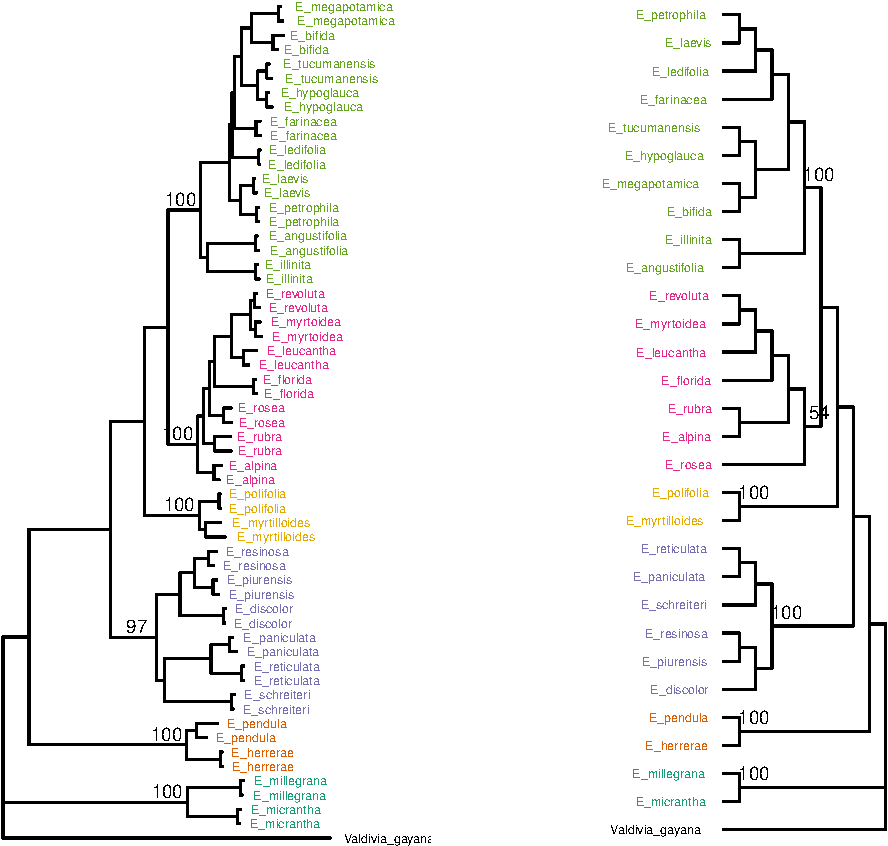
\includegraphics{Supplemental_Material_files/figure-latex/EscalloniaSpeciesTreeTrimmedPlot-1} \caption{Phylogenetic trees of \textit{Escallonia}. Left: Maximum likelihood tree using two specimens per taxonomic species and 364 concatenated loci. Right: Quartet-based species tree. In both trees, colors indicate clades I to VI from bottom to top. Bootstrap support values for focal clades is shown above corresponding bipartition.}\label{fig:EscalloniaSpeciesTreeTrimmedPlot}
\end{figure}

Return to \protect\hyperlink{current-state-of-taxonomic-species-using-genomics-data}{Current state of taxonomic species using genomics data}
\pagebreak

\hypertarget{fig-s2-phylogenetic-trees-four-specimens-per-taxonomic-species}{%
\subsubsection{Fig S2: Phylogenetic trees (four specimens per taxonomic species)}\label{fig-s2-phylogenetic-trees-four-specimens-per-taxonomic-species}}

\begin{figure}
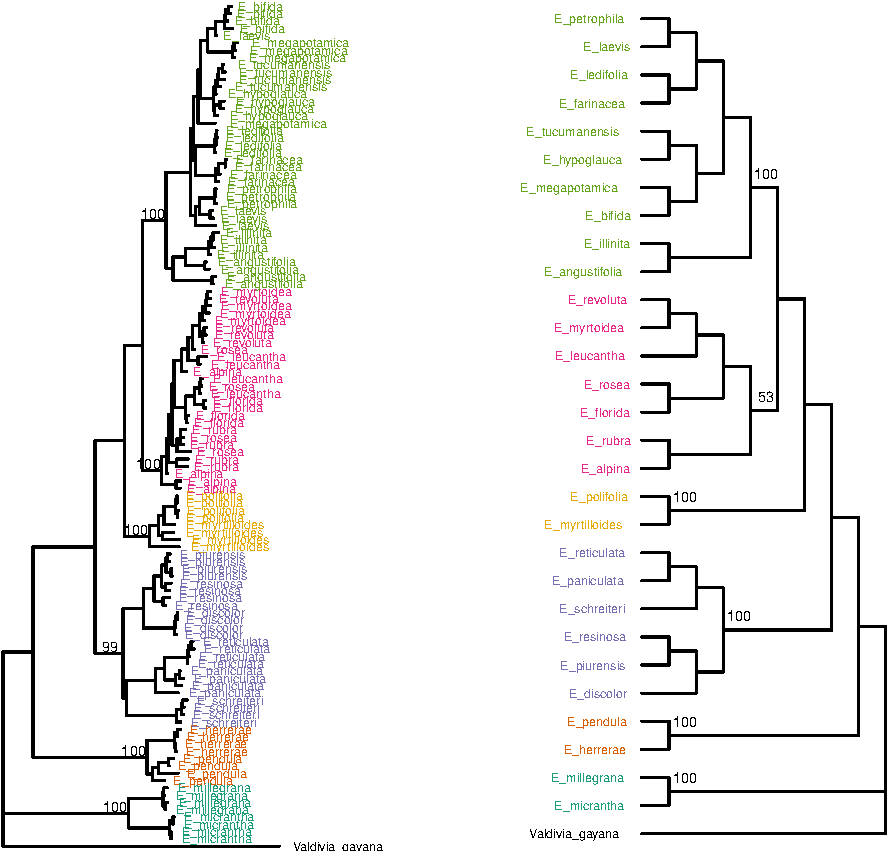
\includegraphics{Supplemental_Material_files/figure-latex/EscalloniaSpeciesTreeVersion2Plot-1} \caption{Phylogenetic trees of \textit{Escallonia}. Maximum likelihood tree using four specimens per taxonomic species and 181 concatenated loci (left). Quartet-based species tree (right). In both trees, colors indicate clades I to VI from bottom to top. Bootstrap support values for focal clades is presented (all other bipartitions were also well-supported)}\label{fig:EscalloniaSpeciesTreeVersion2Plot}
\end{figure}

Return to \protect\hyperlink{current-state-of-taxonomic-species-using-genomics-data}{Current state of taxonomic species using genomics data}
\pagebreak

\hypertarget{clade-i-2}{%
\subsection{Clade I}\label{clade-i-2}}

\hypertarget{fig-s3-taxon-sampling}{%
\subsubsection{Fig S3: Taxon sampling}\label{fig-s3-taxon-sampling}}

\begin{figure}

{\centering 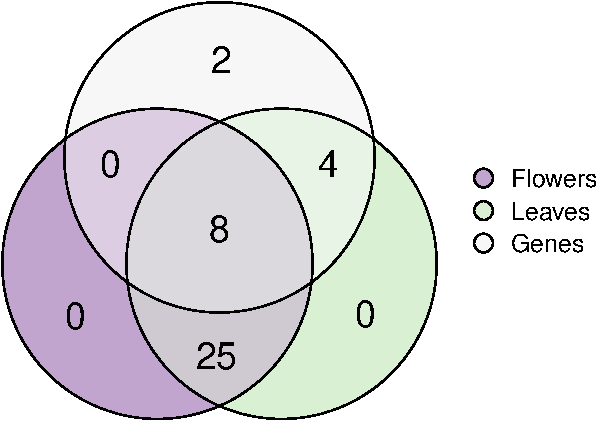
\includegraphics{Supplemental_Material_files/figure-latex/CladeIVennDiagram-1} 

}

\caption{Specimens sampled according to three types of data. Specimens outside the Flowers category represent sterile specimens.}\label{fig:CladeIVennDiagram}
\end{figure}

Return to \protect\hyperlink{sampling-1}{Clade I Sampling}
\pagebreak

\hypertarget{fig-s4-geographic-distribution}{%
\subsubsection{Fig S4: Geographic distribution}\label{fig-s4-geographic-distribution}}

\begin{figure}

{\centering 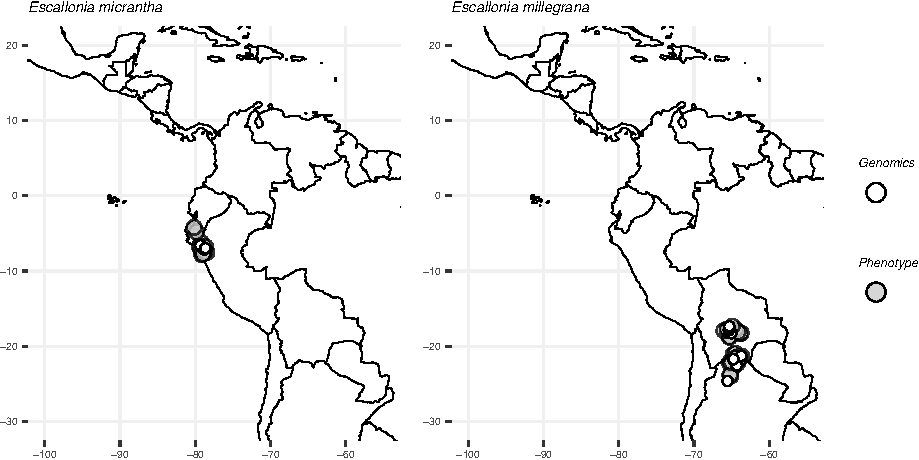
\includegraphics{Supplemental_Material_files/figure-latex/CladeIsamplingMaps-1} 

}

\caption{Geographic distribution of specimens sampled for this clade according to taxonomic species. Filled symbols indicate specimens used in phenotypic analyses and empty symbols specimens used in genomic analyses.}\label{fig:CladeIsamplingMaps}
\end{figure}

Return to \protect\hyperlink{sampling-1}{Clade I Sampling}
\pagebreak

\hypertarget{fig-s5-current-state-of-taxonomic-species-with-phenotypic-data}{%
\subsubsection{Fig S5: Current state of taxonomic species with phenotypic data}\label{fig-s5-current-state-of-taxonomic-species-with-phenotypic-data}}

\begin{figure}
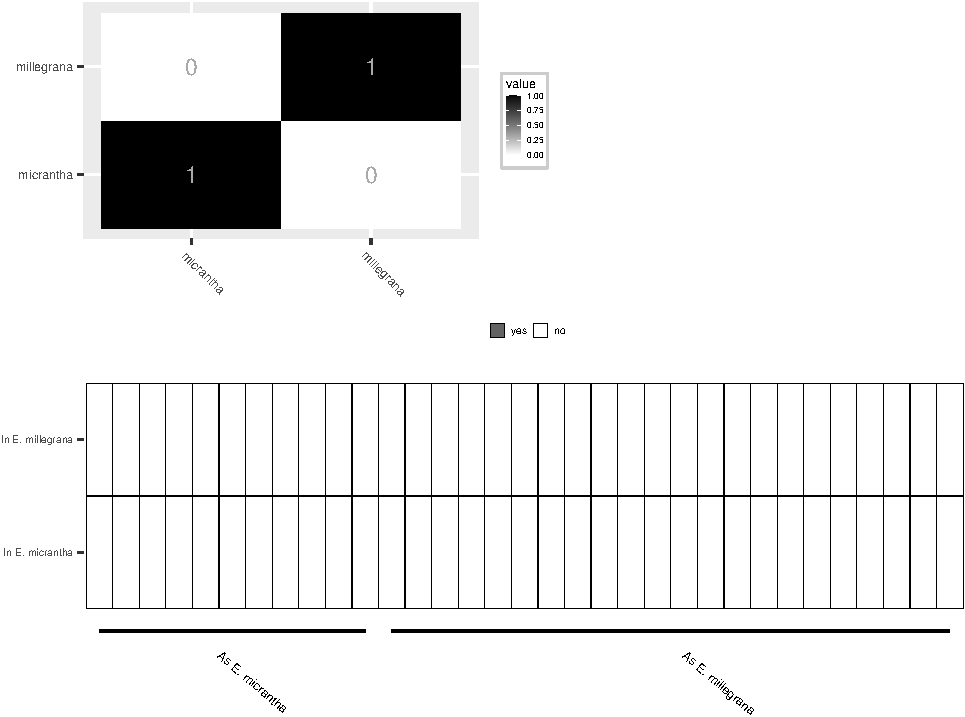
\includegraphics{Supplemental_Material_files/figure-latex/currentStateOfTaxonomyCladeIPlots-1} \caption{Assessment of current state of taxonomic species with phenotypic data. Top panel: Pairwise overlap among 10-cubes describing geometrically each taxonomic species in 10-dimensional phenospace. Bottom panel: Matching-prediction analysis with each cell along the x-axis representing specimens sorted according to taxonomic species and the 10-cubes corresponding to each taxonomic species along the y-axis. If a specimen matches the prediction of the monograph (i.e., it is inside a 10-cube), the corresponding cell is shaded. If the specimen does not match the prediction, the cell is empty.}\label{fig:currentStateOfTaxonomyCladeIPlots}
\end{figure}

Return to \protect\hyperlink{current-state-of-taxonomic-species}{Clade I Current state of taxonomic species}
\pagebreak

\hypertarget{fig-s6-phenogroup-delimitation-gaussian-finite-mixture-modeling}{%
\subsubsection{Fig S6: Phenogroup delimitation: Gaussian finite mixture modeling}\label{fig-s6-phenogroup-delimitation-gaussian-finite-mixture-modeling}}

\begin{figure}
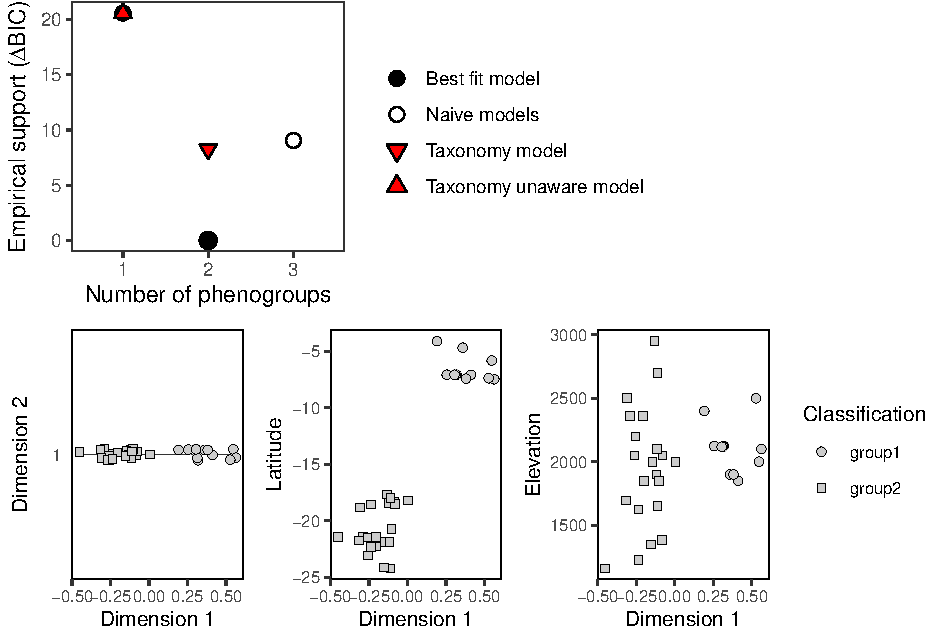
\includegraphics{Supplemental_Material_files/figure-latex/cladeImorphologicalDelimitationPlots-1} \caption{Gaussian finite mixture modeling (GFMM) for phenogroup delimitation and model selection using the Bayesian information criterion (BIC). Top panel: empirical support (ordinate) for Gaussian mixture models (GMM) assuming distinct number of phenogroups (abscissa). Each GMM specifies different number of phenogroups (shapes). Empirical support was measured as difference in BIC relative to the best model ($\Delta$BIC = $0$). Bottom panel: Visualization of the phenogroups (shapes) identified by the best fit GMM; left panel shows phenogroups in the space defined by two axes obtained by linear discriminat analysis (to maximize separation and visualization), middle panel shows phenogroups in the space defined by discriminant axis 1 and latitude, and right panel shows phenogroups in the space defined by discriminant axis 1 and elevation.}\label{fig:cladeImorphologicalDelimitationPlots}
\end{figure}

Return to \protect\hyperlink{model-based-species-discovery}{Clade I Phenomics: model-based species discovery}
\pagebreak

\hypertarget{fig-s7-sensitivity-tests-with-75-missing-data}{%
\subsubsection{\texorpdfstring{Fig S7: Sensitivity tests with \(75\%\) missing data}{Fig S7: Sensitivity tests with 75\textbackslash\% missing data}}\label{fig-s7-sensitivity-tests-with-75-missing-data}}

\begin{figure}
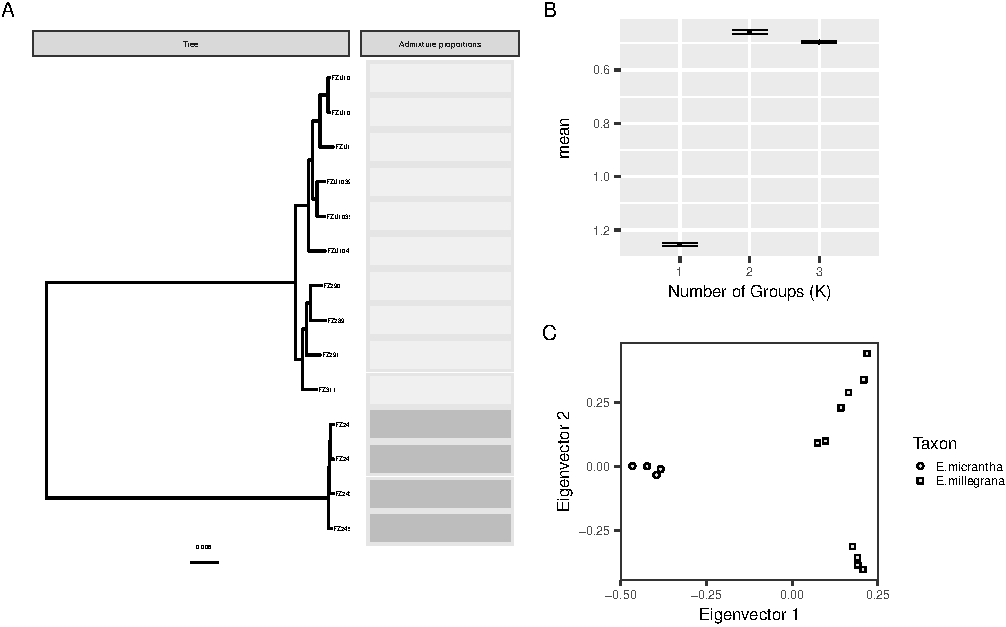
\includegraphics{Supplemental_Material_files/figure-latex/cladeIgenomicSensitivityAnalysesLargestplots-1} \caption{Impact of missing data ($75\%$) on data analysis. A) maximum likelihood phylogenetic tree of specimens assigned to demes according to best \texttt{ADMIXTURE} run. B) Mean cross validation error with $95\%$ confidence interval (ordinate) for ten replicate runs of \texttt{ADMIXTURE} assuming differnt number of demes (K) (abscissa); C) Scatterplot of Principal Component Analysis (PCA) projected along the first two axes.}\label{fig:cladeIgenomicSensitivityAnalysesLargestplots}
\end{figure}

Return to \protect\hyperlink{sensitivity-tests}{Clade I Genomics: sensitivity tests}
\pagebreak

\hypertarget{fig-s8-sensitivity-tests-with-50-missing-data}{%
\subsubsection{\texorpdfstring{Fig S8: Sensitivity tests with \(50\%\) missing data}{Fig S8: Sensitivity tests with 50\textbackslash\% missing data}}\label{fig-s8-sensitivity-tests-with-50-missing-data}}

\begin{figure}
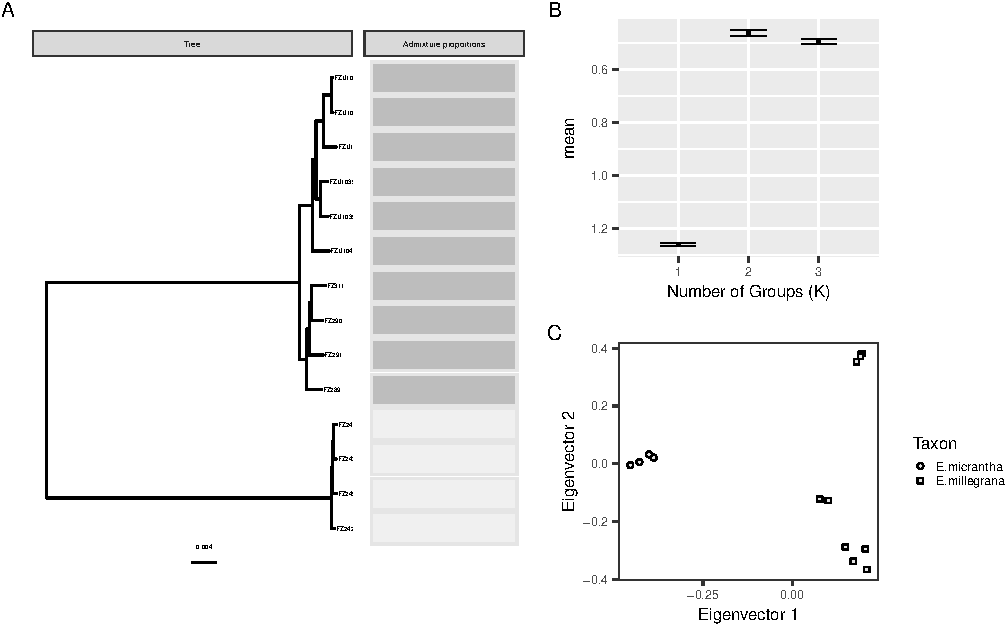
\includegraphics{Supplemental_Material_files/figure-latex/cladeIgenomicSensitivityAnalysesMiddleplots-1} \caption{Impact of missing data ($50\%$) on data analysis. A) maximum likelihood phylogenetic tree of specimens assigned to demes according to best \texttt{ADMIXTURE} run. B) Mean cross validation error with $95\%$ confidence interval (ordinate) for ten replicate runs of \texttt{ADMIXTURE} assuming differnt number of demes (K) (abscissa); C) Scatterplot of Principal Component Analysis (PCA) projected along the first two axes.}\label{fig:cladeIgenomicSensitivityAnalysesMiddleplots}
\end{figure}

Return to \protect\hyperlink{sensitivity-tests}{Clade I Genomics: sensitivity tests}
\pagebreak

\hypertarget{fig-s9-sensitivity-tests-with-25-missing-data}{%
\subsubsection{\texorpdfstring{Fig S9: Sensitivity tests with \(25\%\) missing data}{Fig S9: Sensitivity tests with 25\textbackslash\% missing data}}\label{fig-s9-sensitivity-tests-with-25-missing-data}}

\begin{figure}
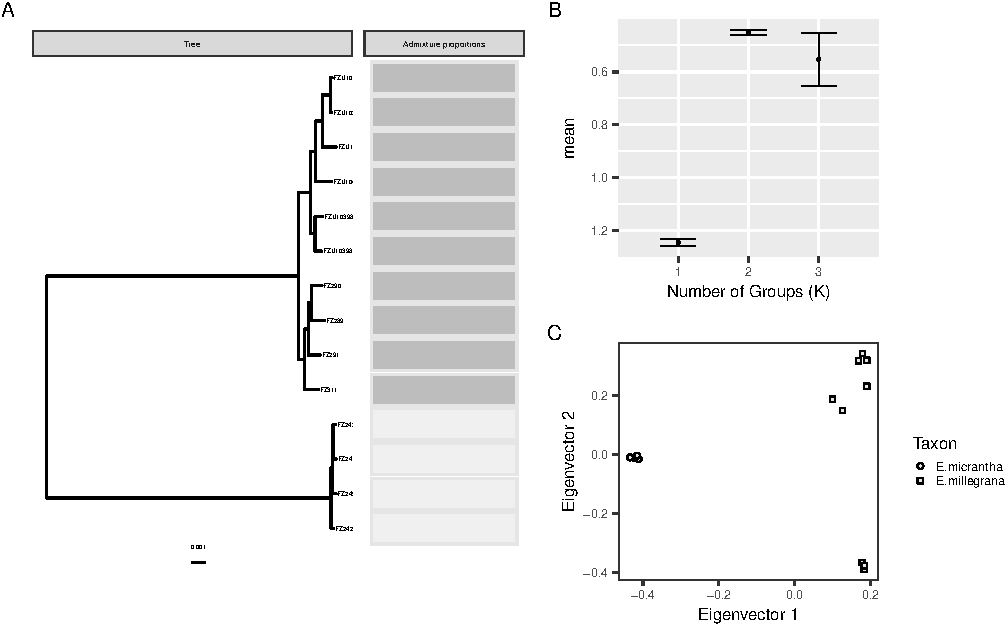
\includegraphics{Supplemental_Material_files/figure-latex/cladeIgenomicSensitivityAnalysesSmallestplots-1} \caption{Impact of missing data ($25\%$) on data analysis. A) maximum likelihood phylogenetic tree of specimens assigned to demes according to best \texttt{ADMIXTURE} run. B) Mean cross validation error with $95\%$ confidence interval (ordinate) for ten replicate runs of \texttt{ADMIXTURE} assuming differnt number of demes (K) (abscissa); C) Scatterplot of Principal Component Analysis (PCA) projected along the first two axes.}\label{fig:cladeIgenomicSensitivityAnalysesSmallestplots}
\end{figure}

Return to \protect\hyperlink{sensitivity-tests}{Clade I Genomics: sensitivity tests}
\pagebreak

\hypertarget{fig-s10-genogroup-delimitation-genotypic-cluster-model}{%
\subsubsection{Fig S10: Genogroup delimitation: Genotypic cluster model}\label{fig-s10-genogroup-delimitation-genotypic-cluster-model}}

\begin{figure}
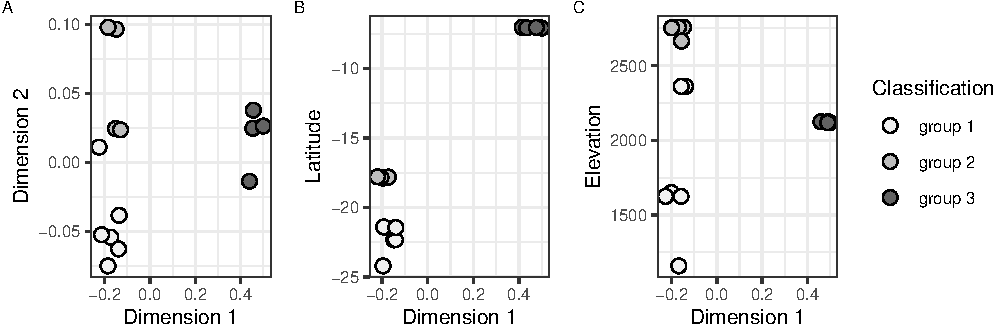
\includegraphics{Supplemental_Material_files/figure-latex/cladeImolecularDelimitationsNmms-1} \caption{Gaussian finite mixture modeling (GFMM) for genogroup delimitation. Visualization of the genogroups (shades) identified by the best fit Gaussian mixture model (GMM). A) genogroups in the space defined by two axes obtained by non-metric multidimensional scaling (NMDS); B) genogroups in the space defined by NMDS axis 1 and latitude; C) genogroups in the space defined by NMDS axis 1 and elevation.}\label{fig:cladeImolecularDelimitationsNmms}
\end{figure}

Return to \protect\hyperlink{model-based-species-discovery-1}{Clade I Genomics: model-based species discovery}
\pagebreak

\hypertarget{fig-s11-genogroup-delimitation.-cladogenesis-to-anagenesis-model}{%
\subsubsection{Fig S11: Genogroup delimitation. Cladogenesis to anagenesis model}\label{fig-s11-genogroup-delimitation.-cladogenesis-to-anagenesis-model}}

\begin{figure}
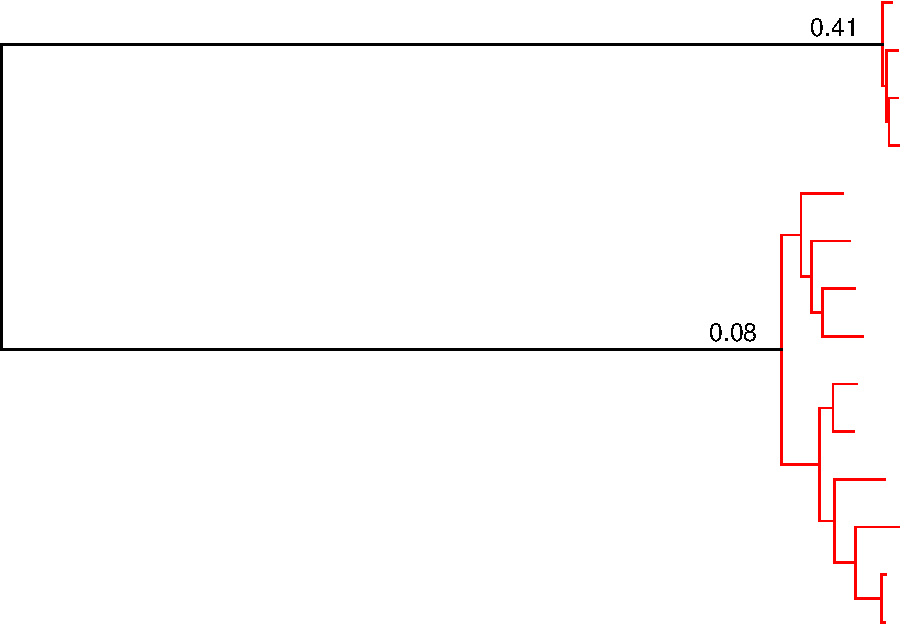
\includegraphics[height=.6\textwidth,]{Supplemental_Material_files/figure-latex/cladeImolecularDelimitationsPhylogeny2-1} \caption{Phylogenetic modeling for genogroup delimitation. Midpoint-rooted phylogenetic tree showing genogroups in red. Values correspond to nodes at the transition point between cladogenesis (between species) to anagenesis (within species). Values closer to 0 indicate that the node was identified as a transition to anagenesis summarized over $500$ delimitations.}\label{fig:cladeImolecularDelimitationsPhylogeny2}
\end{figure}

Return to \protect\hyperlink{model-based-species-discovery-1}{Clade I Genomics: model-based species discovery}
\pagebreak

\hypertarget{fig-s12-genogroup-delimitation-reproductive-isolation-model}{%
\subsubsection{Fig S12: Genogroup delimitation: Reproductive isolation model}\label{fig-s12-genogroup-delimitation-reproductive-isolation-model}}

\begin{figure}
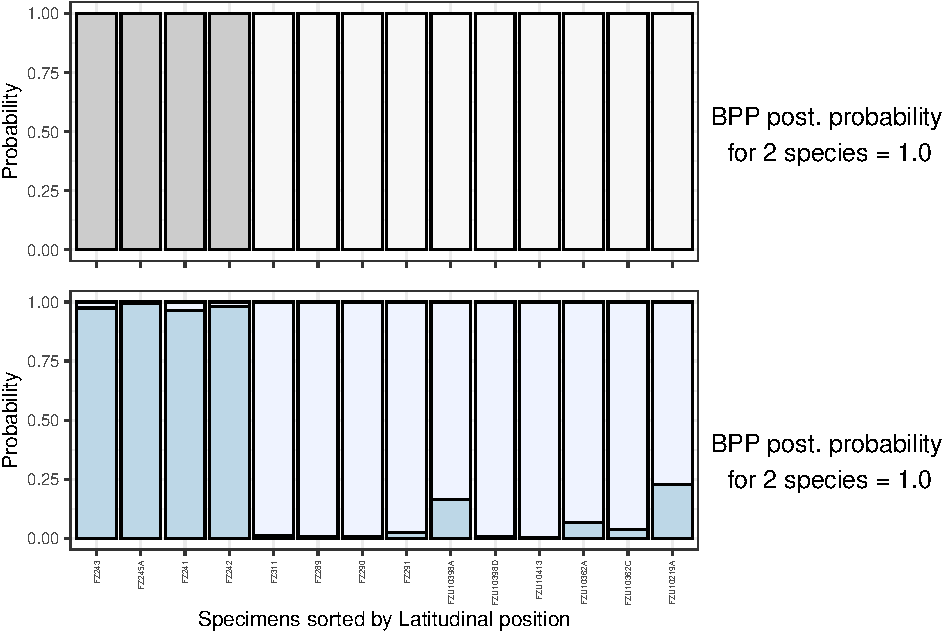
\includegraphics{Supplemental_Material_files/figure-latex/cladeImolecularDelimitationPopGenBpp-1} \caption{Population genetic modeling for genogroup delimitation. Top panel: assignment of specimens to demes according to \texttt{STRUCTURE} and posterior probability of species delimitation modeling according to \texttt{BPP} using these demes. Bottom panel: assignment of specimens to demes according to \texttt{MAVERICK} and posterior probability of species delimitation modeling according to \texttt{BPP} using these demes. Specimens are sorted from north (left) to south (right) according to locality of collection.}\label{fig:cladeImolecularDelimitationPopGenBpp}
\end{figure}

Return to \protect\hyperlink{model-based-species-discovery-1}{Clade I Genomics: model-based species discovery}
\pagebreak

\hypertarget{fig-s13-data-integration}{%
\subsubsection{Fig S13: Data integration}\label{fig-s13-data-integration}}

\begin{figure}
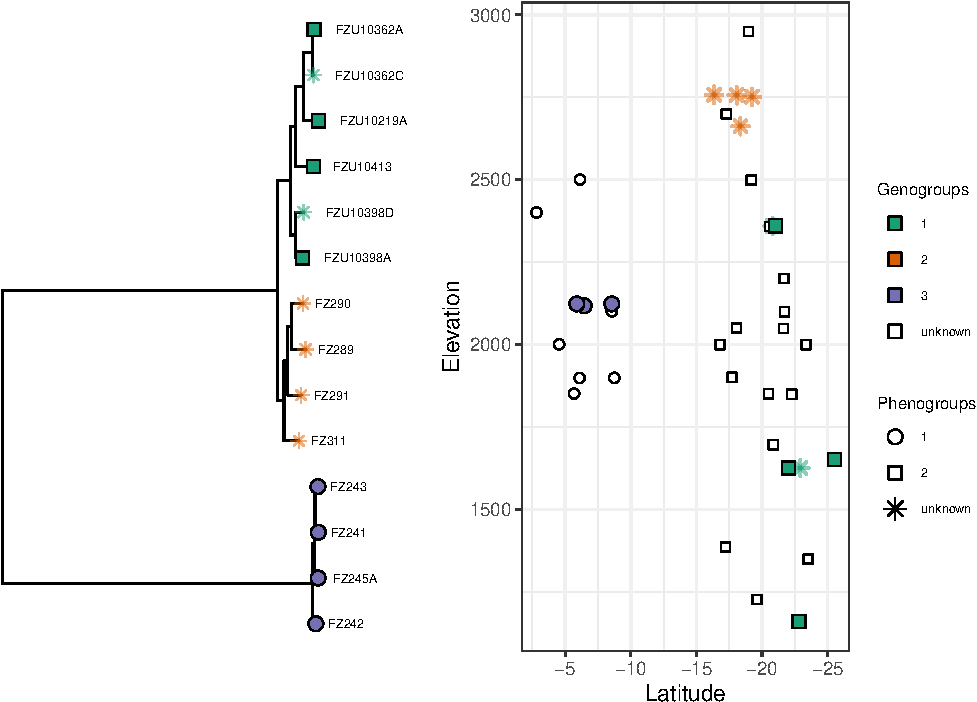
\includegraphics{Supplemental_Material_files/figure-latex/cladeIfinalDelimitation2-1} \caption{Integration of phenotypic and genomic data with spatial information and evolutionary history. All specimens are assigned to their corresponding best fit phenogroup (shapes) and genogroup (colors). Specimens without phenotypic or genomic data (unknown specimens) are shown as asterisks and empty shapes, accordingly. Specimens are shown as tips of the maximum likelihood tree (left) used in the CA model analysis and mapped along latitude and elevation (right). Specimens assigned to a single phenogroup and a single genogroup delineate species that we determined as 'good species'. Specimens assigned to a single phenogroup across multiple genogroups delineate species that we determined as 'phenotypic cryptic species'. Specimens assigned to a single genogroup across multiple phenogroups delineate species that we determined as 'genetic cryptic species'.}\label{fig:cladeIfinalDelimitation2}
\end{figure}

Return to \protect\hyperlink{data-integration-1}{Clade I Data integration}
\pagebreak

\hypertarget{clade-ii-2}{%
\subsection{Clade II}\label{clade-ii-2}}

\hypertarget{fig-s14-taxon-sampling}{%
\subsubsection{Fig S14: Taxon sampling}\label{fig-s14-taxon-sampling}}

\begin{figure}

{\centering 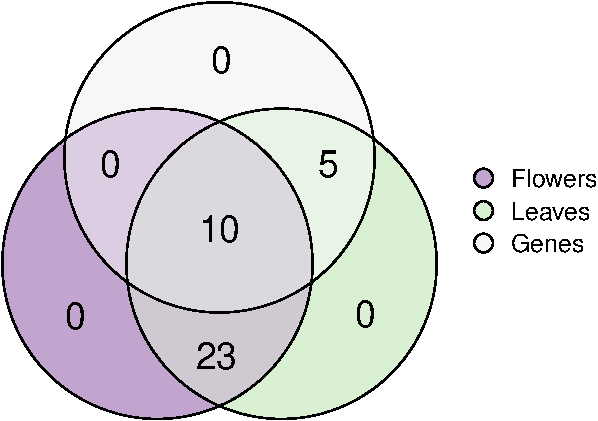
\includegraphics{Supplemental_Material_files/figure-latex/CladeIIVennDiagram-1} 

}

\caption{Specimens sampled according to three types of data. Specimens outside the Flowers category represent sterile specimens.}\label{fig:CladeIIVennDiagram}
\end{figure}

Return to \protect\hyperlink{sampling-2}{Clade II Sampling}
\pagebreak

\hypertarget{fig-s15-geographic-distribution}{%
\subsubsection{Fig S15: Geographic distribution}\label{fig-s15-geographic-distribution}}

\begin{figure}

{\centering 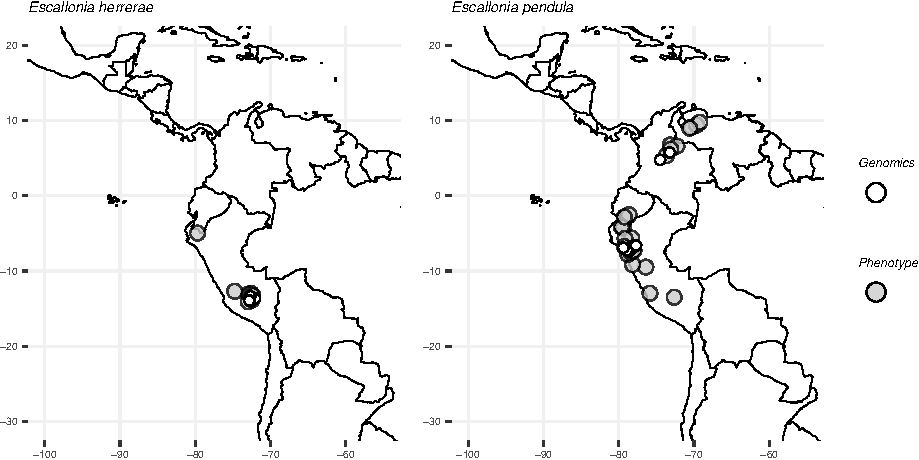
\includegraphics{Supplemental_Material_files/figure-latex/CladeIIsamplingMaps-1} 

}

\caption{Geographic distribution of specimens sampled for this clade according to taxonomic species. Filled symbols indicate specimens used in phenotypic analyses and empty symbols specimens used in genomic analyses.}\label{fig:CladeIIsamplingMaps}
\end{figure}

Return to \protect\hyperlink{sampling-2}{Clade II Sampling}
\pagebreak

\hypertarget{fig-s16-current-state-of-taxonomic-species-with-phenotypic-data}{%
\subsubsection{Fig S16: Current state of taxonomic species with phenotypic data}\label{fig-s16-current-state-of-taxonomic-species-with-phenotypic-data}}

\begin{figure}
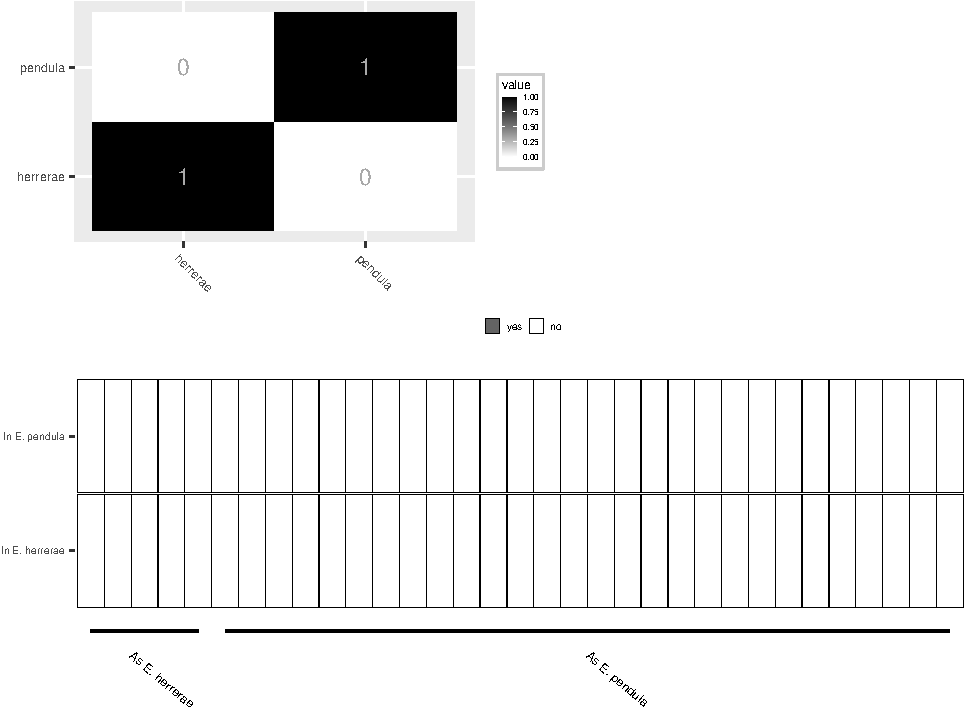
\includegraphics{Supplemental_Material_files/figure-latex/currentStateOfTaxonomyCladeIIPlots-1} \caption{Assessment of current state of taxonomic species with phenotypic data. Top panel: Pairwise overlap among 10-cubes describing geometrically each taxonomic species. Bottom panel: Matching-prediction analysis with each cell along the x-axis representing specimens sorted according to taxonomic species and the 10-cubes corresponding to each taxonomic species along the y-axis. If a specimen matches the prediction of the monograph (i.e., it is inside a 10-cube), the corresponding cell is shaded. If the specimen does not match the prediction, the cell is empty.}\label{fig:currentStateOfTaxonomyCladeIIPlots}
\end{figure}

Return to \protect\hyperlink{current-state-of-taxonomic-species-1}{Clade II Current state of taxonomic species}
\pagebreak

\hypertarget{fig-s17-phenogroup-delimitation-gaussian-finite-mixture-modeling}{%
\subsubsection{Fig S17: Phenogroup delimitation: Gaussian finite mixture modeling}\label{fig-s17-phenogroup-delimitation-gaussian-finite-mixture-modeling}}

\begin{figure}
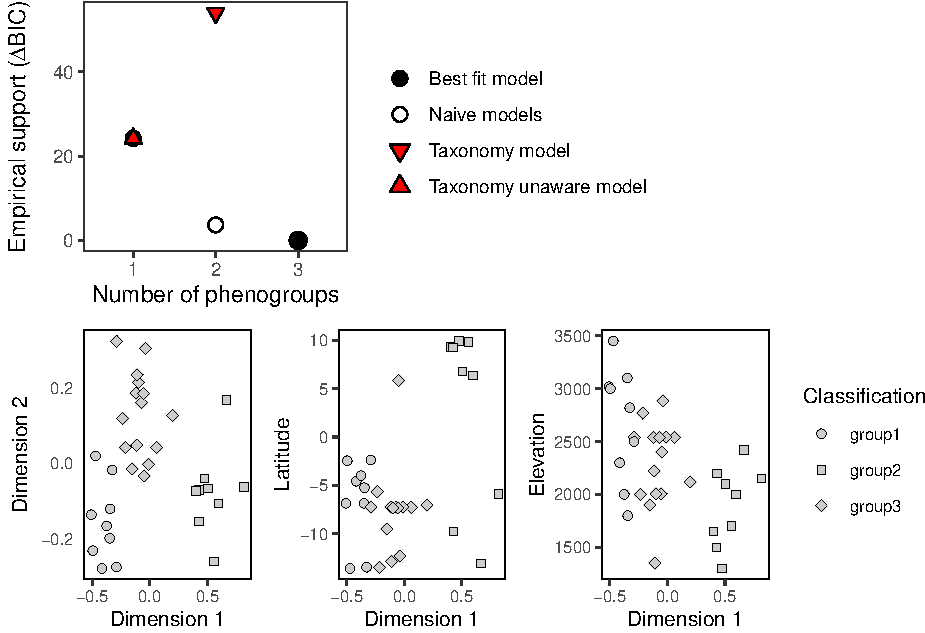
\includegraphics{Supplemental_Material_files/figure-latex/cladeIImorphologicalDelimitationPlots-1} \caption{Gaussian finite mixture modeling (GFMM) for phenogroup delimitation and model selection using the Bayesian information criterion (BIC). Top panel: empirical support (ordinate) for Gaussian mixture models (GMM) assuming distinct number of phenogroups (abscissa). Each GMM specifies different number of phenogroups (shapes). Empirical support was measured as difference in BIC relative to the best model ($\Delta$BIC = $0$). Bottom panel: Visualization of the phenogroups (shapes) identified by the best fit GMM; left panel shows phenogroups in the space defined by two axes obtained by linear discriminat analysis (to maximize separation and visualization), middle panel shows phenogroups in the space defined by discriminant axis 1 and latitude, and right panel shows phenogroups in the space defined by discriminant axis 1 and elevation.}\label{fig:cladeIImorphologicalDelimitationPlots}
\end{figure}

Return to \protect\hyperlink{model-based-species-discovery-2}{Clade II Phenomics: model-based species discovery}
\pagebreak

\hypertarget{fig-s18-sensitivity-tests-with-75-missing-data}{%
\subsubsection{\texorpdfstring{Fig S18: Sensitivity tests with \(75\%\) missing data}{Fig S18: Sensitivity tests with 75\textbackslash\% missing data}}\label{fig-s18-sensitivity-tests-with-75-missing-data}}

\begin{figure}
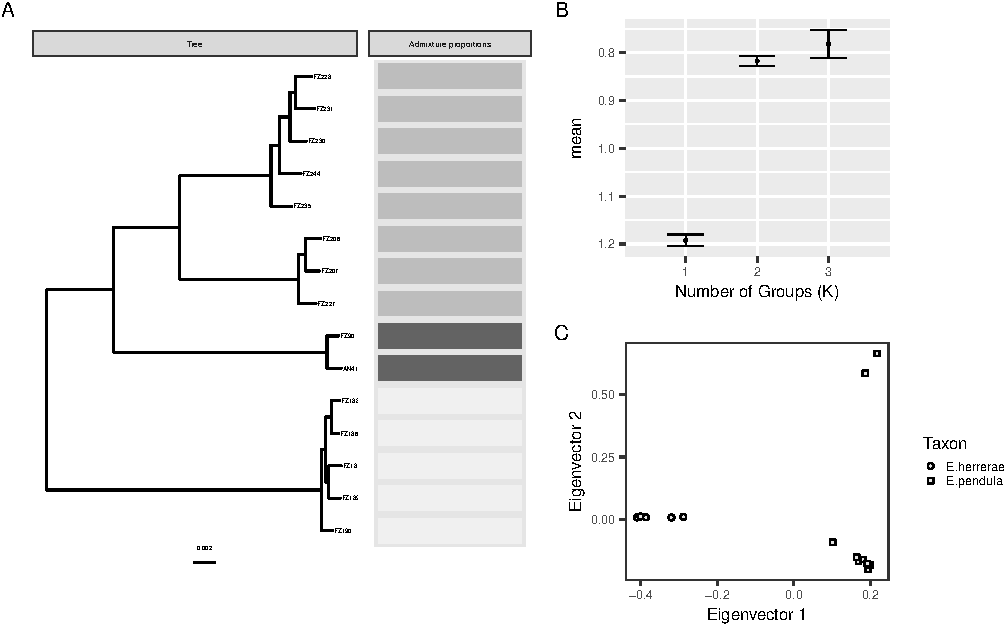
\includegraphics{Supplemental_Material_files/figure-latex/cladeIIgenomicSensitivityAnalysesLargestplots-1} \caption{Impact of missing data ($75\%$) on data analysis. A) maximum likelihood phylogenetic tree of specimens assigned to demes according to best \texttt{ADMIXTURE} run. B) Mean cross validation error with $95\%$ confidence interval (ordinate) for ten replicate runs of \texttt{ADMIXTURE} assuming differnt number of demes (K) (abscissa); C) Scatterplot of Principal Component Analysis (PCA) projected along the first two axes.}\label{fig:cladeIIgenomicSensitivityAnalysesLargestplots}
\end{figure}

Return to \protect\hyperlink{sensitivity-tests-1}{Clade II Genomics: sensitivity tests}
\pagebreak

\hypertarget{fig-s19-sensitivity-tests-with-50-missing-data}{%
\subsubsection{\texorpdfstring{Fig S19: Sensitivity tests with \(50\%\) missing data}{Fig S19: Sensitivity tests with 50\textbackslash\% missing data}}\label{fig-s19-sensitivity-tests-with-50-missing-data}}

\begin{figure}
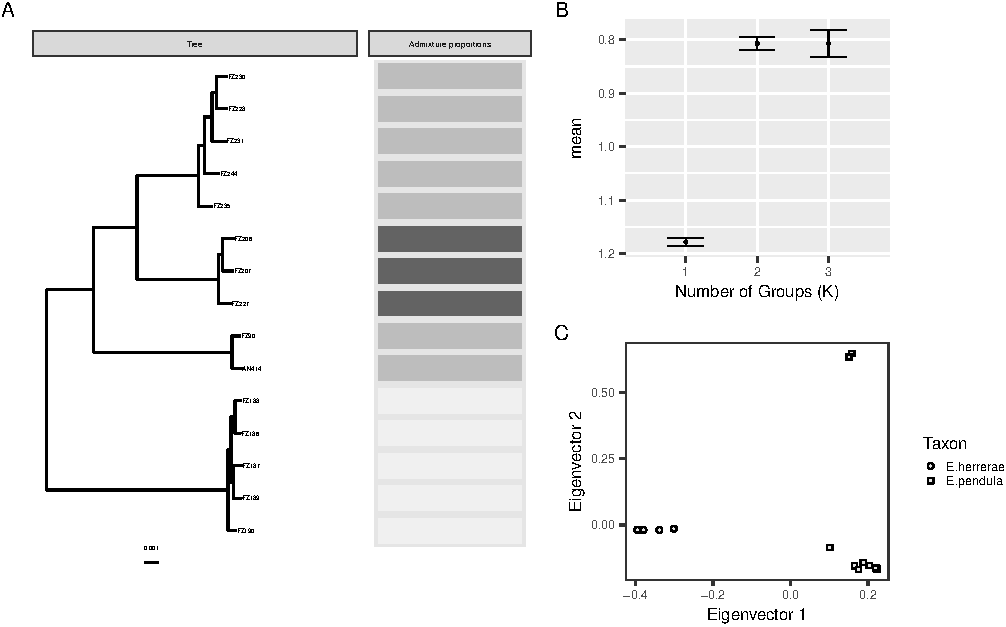
\includegraphics{Supplemental_Material_files/figure-latex/cladeIIgenomicSensitivityAnalysesMiddleplots-1} \caption{Impact of missing data ($50\%$) on data analysis. A) maximum likelihood phylogenetic tree of specimens assigned to demes according to best \texttt{ADMIXTURE} run. B) Mean cross validation error with $95\%$ confidence interval (ordinate) for ten replicate runs of \texttt{ADMIXTURE} assuming differnt number of demes (K) (abscissa); C) Scatterplot of Principal Component Analysis (PCA) projected along the first two axes.}\label{fig:cladeIIgenomicSensitivityAnalysesMiddleplots}
\end{figure}

Return to \protect\hyperlink{sensitivity-tests-1}{Clade II Genomics: sensitivity tests}
\pagebreak

\hypertarget{fig-s20-sensitivity-tests-with-25-missing-data}{%
\subsubsection{\texorpdfstring{Fig S20: Sensitivity tests with \(25\%\) missing data}{Fig S20: Sensitivity tests with 25\textbackslash\% missing data}}\label{fig-s20-sensitivity-tests-with-25-missing-data}}

\begin{figure}
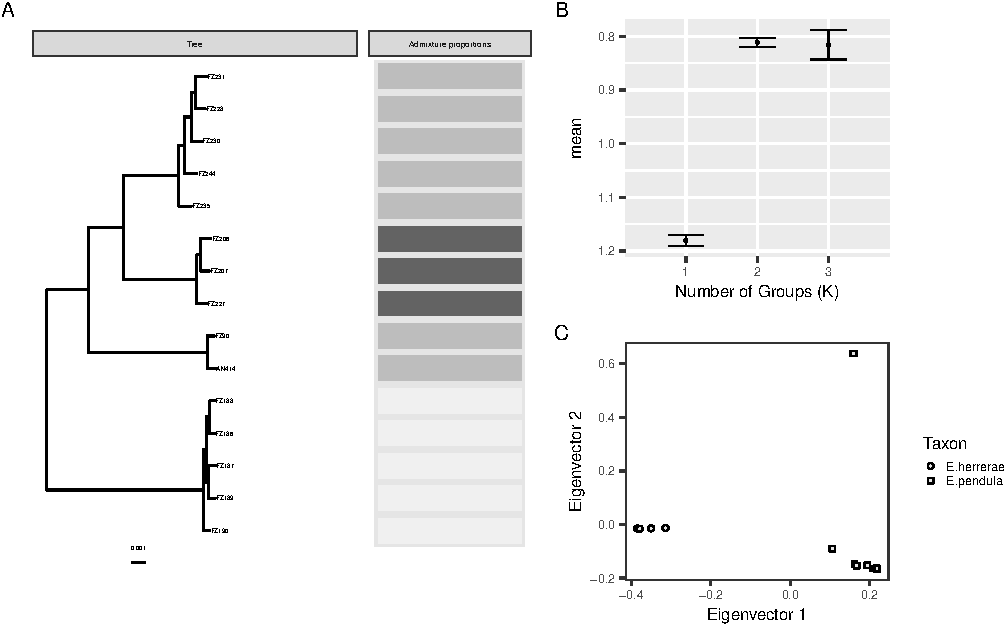
\includegraphics{Supplemental_Material_files/figure-latex/cladeIIgenomicSensitivityAnalysesSmallestplots-1} \caption{Impact of missing data ($25\%$) on data analysis. A) maximum likelihood phylogenetic tree of specimens assigned to demes according to best \texttt{ADMIXTURE} run. B) Mean cross validation error with $95\%$ confidence interval (ordinate) for ten replicate runs of \texttt{ADMIXTURE} assuming differnt number of demes (K) (abscissa); C) Scatterplot of Principal Component Analysis (PCA) projected along the first two axes.}\label{fig:cladeIIgenomicSensitivityAnalysesSmallestplots}
\end{figure}

Return to \protect\hyperlink{sensitivity-tests-1}{Clade II Genomics: sensitivity tests}
\pagebreak

\hypertarget{fig-s21-genogroup-delimitation-genotypic-cluster-model}{%
\subsubsection{Fig S21: Genogroup delimitation: Genotypic cluster model}\label{fig-s21-genogroup-delimitation-genotypic-cluster-model}}

\begin{figure}
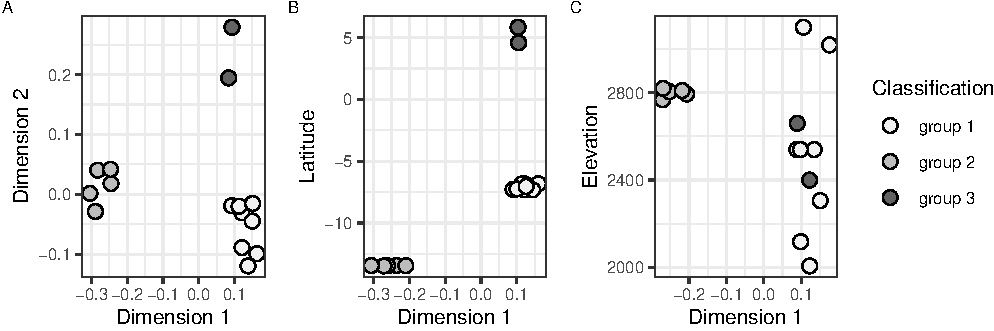
\includegraphics{Supplemental_Material_files/figure-latex/cladeIImolecularDelimitationsNmms-1} \caption{Gaussian finite mixture modeling (GFMM) for genogroup delimitation. Visualization of the genogroups (shades) identified by the best fit Gaussian mixture model (GMM). A) genogroups in the space defined by two axes obtained by non-metric multidimensional scaling (NMDS); B) genogroups in the space defined by NMDS axis 1 and latitude; C) genogroups in the space defined by NMDS axis 1 and elevation.}\label{fig:cladeIImolecularDelimitationsNmms}
\end{figure}

Return to \protect\hyperlink{model-based-species-discovery-3}{Clade II Genomics: model-based species discovery}
\pagebreak

\hypertarget{fig-s22-genogroup-delimitation.-cladogenesis-to-anagenesis-model}{%
\subsubsection{Fig S22: Genogroup delimitation. Cladogenesis to anagenesis model}\label{fig-s22-genogroup-delimitation.-cladogenesis-to-anagenesis-model}}

\begin{figure}
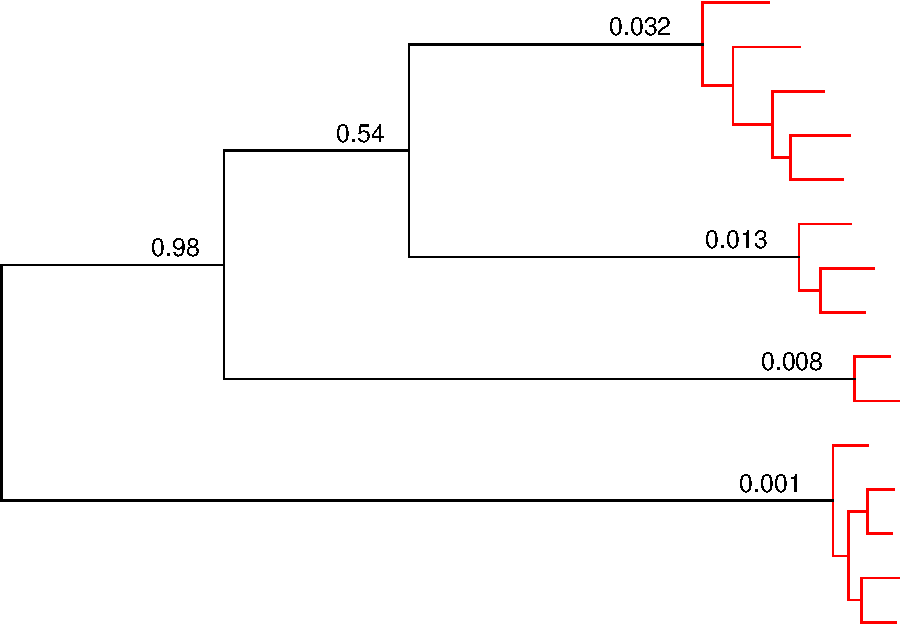
\includegraphics[height=.6\textwidth,]{Supplemental_Material_files/figure-latex/cladeIImolecularDelimitationsPhylogeny2-1} \caption{Phylogenetic modeling for genogroup delimitation. Midpoint-rooted phylogenetic tree showing genogroups in red. Values correspond to nodes at the transition point between cladogenesis (between species) to anagenesis (within species). Values closer to 0 indicate that the node was identified as a transition to anagenesis summarized over $500$ delimitations.}\label{fig:cladeIImolecularDelimitationsPhylogeny2}
\end{figure}

Return to \protect\hyperlink{model-based-species-discovery-3}{Clade II Genomics: model-based species discovery}
\pagebreak

\hypertarget{fig-s23-genogroup-delimitation-reproductive-isolation-model}{%
\subsubsection{Fig S23: Genogroup delimitation: Reproductive isolation model}\label{fig-s23-genogroup-delimitation-reproductive-isolation-model}}

\begin{figure}
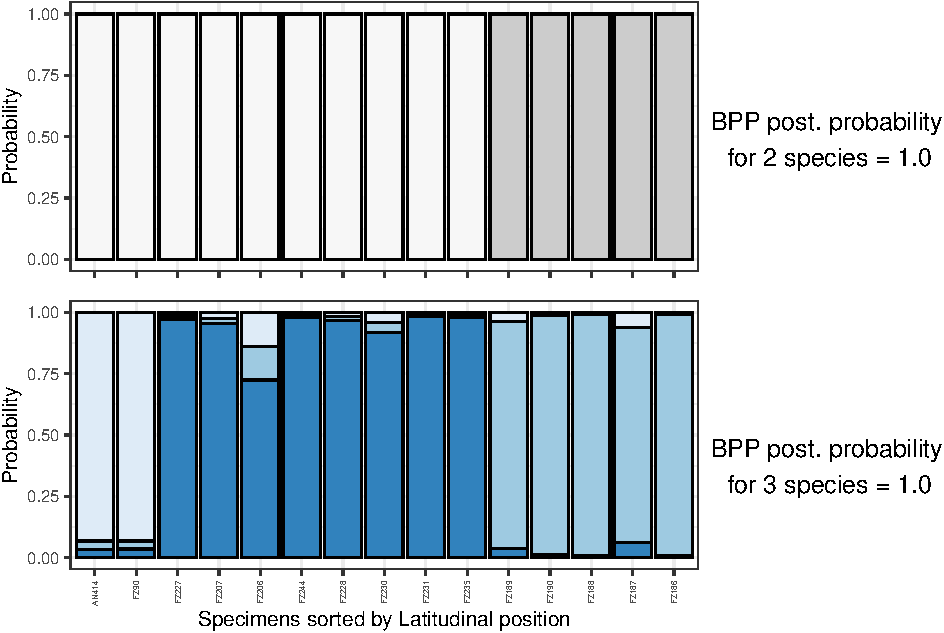
\includegraphics{Supplemental_Material_files/figure-latex/cladeIImolecularDelimitationPopGenBpp-1} \caption{Population genetic modeling for genogroup delimitation. Top panel: assignment of specimens to demes according to \texttt{STRUCTURE} and posterior probability of species delimitation modeling according to \texttt{BPP} using these demes. Bottom panel: assignment of specimens to demes according to \texttt{MAVERICK} and posterior probability of species delimitation modeling according to \texttt{BPP} using these demes. Specimens are sorted from north (left) to south (right) according to locality of collection.}\label{fig:cladeIImolecularDelimitationPopGenBpp}
\end{figure}

Return to \protect\hyperlink{model-based-species-discovery-3}{Clade II Genomics: model-based species discovery}
\pagebreak

\hypertarget{fig-s24-data-integration}{%
\subsubsection{Fig S24: Data integration}\label{fig-s24-data-integration}}

\begin{figure}
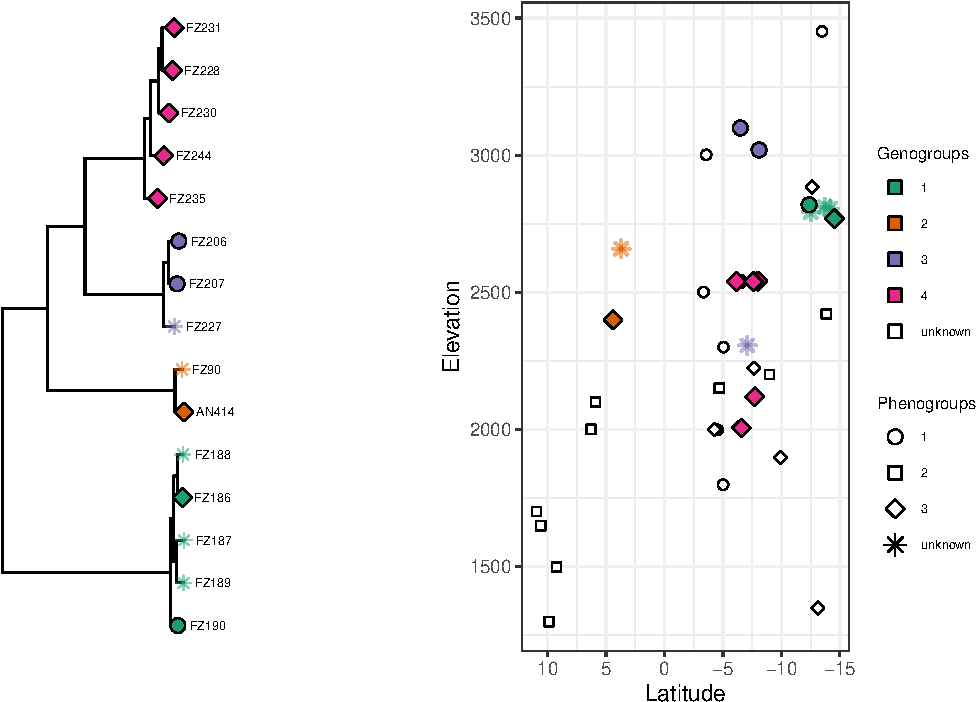
\includegraphics{Supplemental_Material_files/figure-latex/cladeIIfinalDelimitation2-1} \caption{Integration of phenotypic and genomic data with spatial information and evolutionary history. All specimens are assigned to their corresponding best fit phenogroup (shapes) and genogroup (colors). Specimens without phenotypic or genomic data (unknown specimens) are shown as asterisks and empty shapes, accordingly. Specimens are shown as tips of the maximum likelihood tree (left) used in the CA model analysis and mapped along latitude and elevation (right). Specimens assigned to a single phenogroup and a single genogroup delineate species that we determined as 'good species'. Specimens assigned to a single phenogroup across multiple genogroups delineate species that we determined as 'phenotypic cryptic species'. Specimens assigned to a single genogroup across multiple phenogroups delineate species that we determined as 'genetic cryptic species'.}\label{fig:cladeIIfinalDelimitation2}
\end{figure}

Return to \protect\hyperlink{data-integration-2}{Clade II Data integration}
\pagebreak

\hypertarget{clade-iii-2}{%
\subsection{Clade III}\label{clade-iii-2}}

\hypertarget{fig-s25-taxon-sampling}{%
\subsubsection{Fig S25: Taxon sampling}\label{fig-s25-taxon-sampling}}

\begin{figure}

{\centering 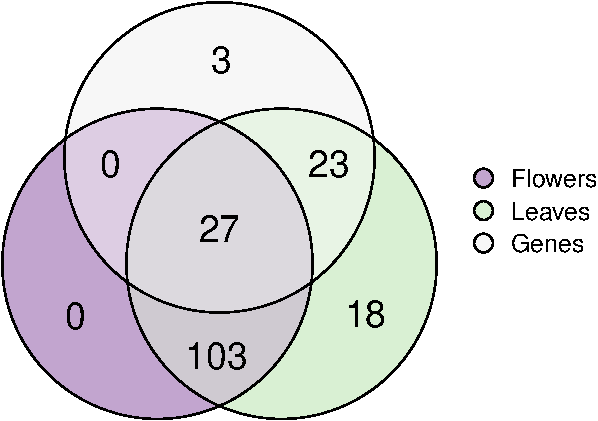
\includegraphics{Supplemental_Material_files/figure-latex/CladeIIIVennDiagram-1} 

}

\caption{Specimens sampled according to three types of data. Specimens outside the Flowers category represent sterile specimens.}\label{fig:CladeIIIVennDiagram}
\end{figure}

Return to \protect\hyperlink{sampling-3}{Clade III Sampling}
\pagebreak

\hypertarget{fig-s26-geographic-distribution}{%
\subsubsection{Fig S26: Geographic distribution}\label{fig-s26-geographic-distribution}}

\begin{figure}

{\centering 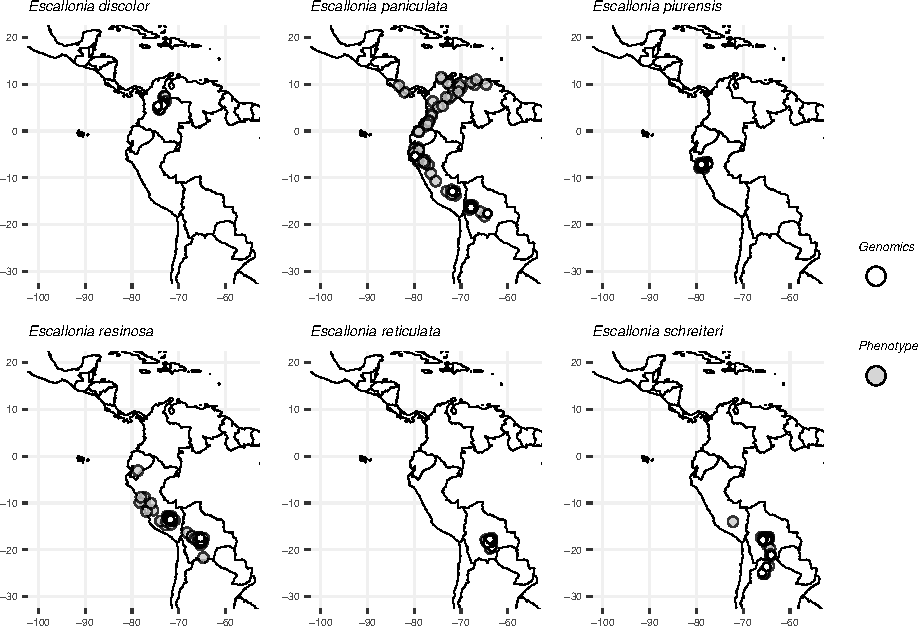
\includegraphics{Supplemental_Material_files/figure-latex/CladeIIIsamplingMaps-1} 

}

\caption{Geographic distribution of specimens sampled for this clade according to taxonomic species. Filled symbols indicate specimens used in phenotypic analyses and empty symbols specimens used in genomic analyses.}\label{fig:CladeIIIsamplingMaps}
\end{figure}

Return to \protect\hyperlink{sampling-3}{Clade III Sampling}
\pagebreak

\hypertarget{fig-s27-current-state-of-taxonomic-species-with-phenotypic-data}{%
\subsubsection{Fig S27: Current state of taxonomic species with phenotypic data}\label{fig-s27-current-state-of-taxonomic-species-with-phenotypic-data}}

\begin{figure}
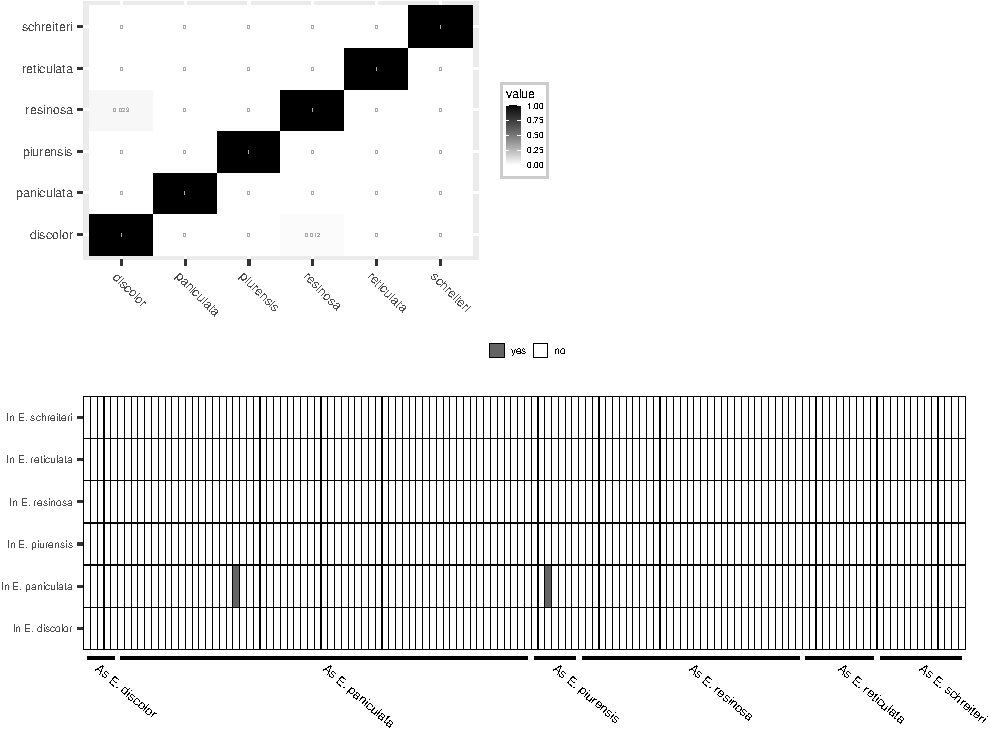
\includegraphics{Supplemental_Material_files/figure-latex/currentStateOfTaxonomyCladeIIIPlots-1} \caption{Assessment of current state of taxonomic species with phenotypic data. Top panel: Pairwise overlap among 10-cubes describing geometrically each taxonomic species. Bottom panel: Matching-prediction analysis with each cell along the x-axis representing specimens sorted according to taxonomic species and the 10-cubes corresponding to each taxonomic species along the y-axis. If a specimen matches the prediction of the monograph (i.e., it is inside a 10-cube), the corresponding cell is shaded. If the specimen does not match the prediction, the cell is empty.}\label{fig:currentStateOfTaxonomyCladeIIIPlots}
\end{figure}

Return to \protect\hyperlink{current-state-of-taxonomic-species-2}{Clade III Current state of taxonomic species}
\pagebreak

\hypertarget{fig-s28-phenogroup-delimitation-gaussian-finite-mixture-modeling}{%
\subsubsection{Fig S28: Phenogroup delimitation: Gaussian finite mixture modeling}\label{fig-s28-phenogroup-delimitation-gaussian-finite-mixture-modeling}}

\begin{figure}
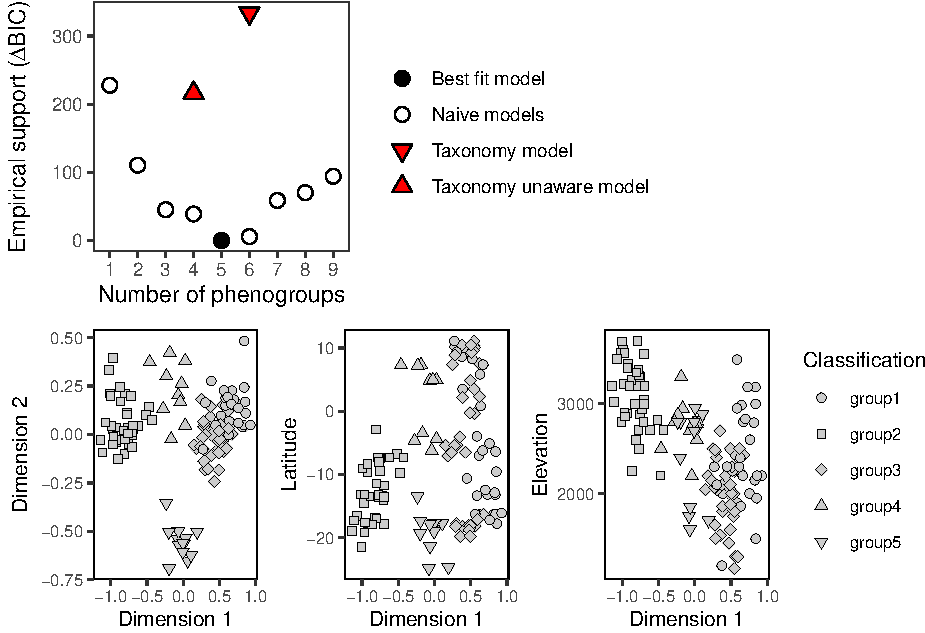
\includegraphics{Supplemental_Material_files/figure-latex/cladeIIImorphologicalDelimitationPlots-1} \caption{Gaussian finite mixture modeling (GFMM) for phenogroup delimitation and model selection using the Bayesian information criterion (BIC). Top panel: empirical support (ordinate) for Gaussian mixture models (GMM) assuming distinct number of phenogroups (abscissa). Each GMM specifies different number of phenogroups (shapes). Empirical support was measured as difference in BIC relative to the best model ($\Delta$BIC = $0$). Bottom panel: Visualization of the phenogroups (shapes) identified by the best fit GMM; left panel shows phenogroups in the space defined by two axes obtained by linear discriminat analysis (to maximize separation and visualization), middle panel shows phenogroups in the space defined by discriminant axis 1 and latitude, and right panel shows phenogroups in the space defined by discriminant axis 1 and elevation.}\label{fig:cladeIIImorphologicalDelimitationPlots}
\end{figure}

Return to \protect\hyperlink{model-based-species-discovery-4}{Clade III Phenomics: model-based species discovery}
\pagebreak

\hypertarget{fig-s29-sensitivity-tests-with-75-missing-data}{%
\subsubsection{\texorpdfstring{Fig S29: Sensitivity tests with \(75\%\) missing data}{Fig S29: Sensitivity tests with 75\textbackslash\% missing data}}\label{fig-s29-sensitivity-tests-with-75-missing-data}}

\begin{figure}
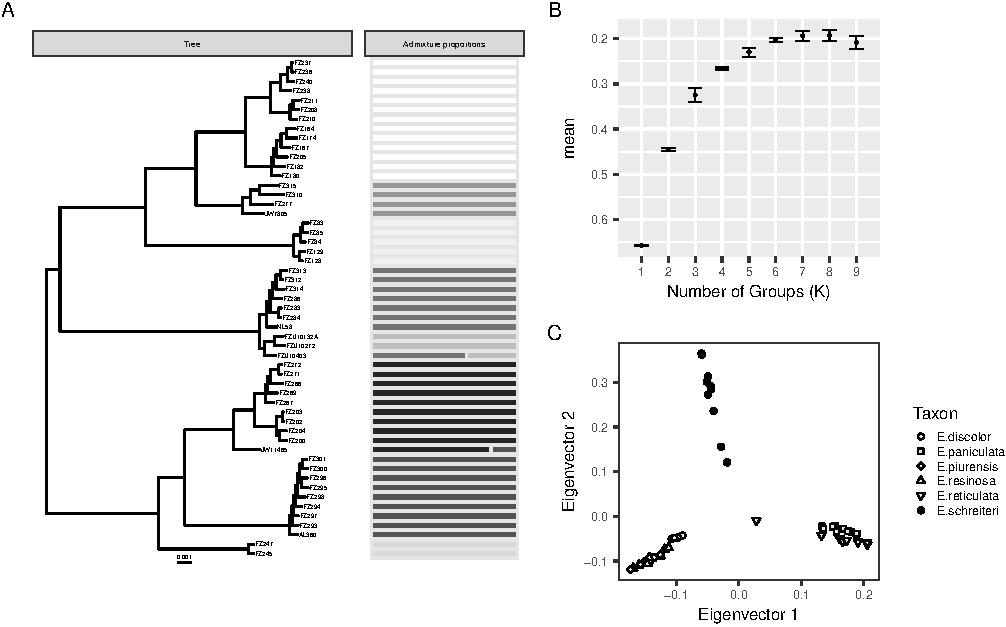
\includegraphics{Supplemental_Material_files/figure-latex/cladeIIIgenomicSensitivityAnalysesLargestplots-1} \caption{Impact of missing data ($75\%$) on data analysis. A) maximum likelihood phylogenetic tree of specimens assigned to demes according to best \texttt{ADMIXTURE} run. B) Mean cross validation error with $95\%$ confidence interval (ordinate) for ten replicate runs of \texttt{ADMIXTURE} assuming differnt number of demes (K) (abscissa); C) Scatterplot of Principal Component Analysis (PCA) projected along the first two axes.}\label{fig:cladeIIIgenomicSensitivityAnalysesLargestplots}
\end{figure}

Return to \protect\hyperlink{sensitivity-tests-2}{Clade III Genomics: sensitivity tests}
\pagebreak

\hypertarget{fig-s30-sensitivity-tests-with-50-missing-data}{%
\subsubsection{\texorpdfstring{Fig S30: Sensitivity tests with \(50\%\) missing data}{Fig S30: Sensitivity tests with 50\textbackslash\% missing data}}\label{fig-s30-sensitivity-tests-with-50-missing-data}}

\begin{figure}
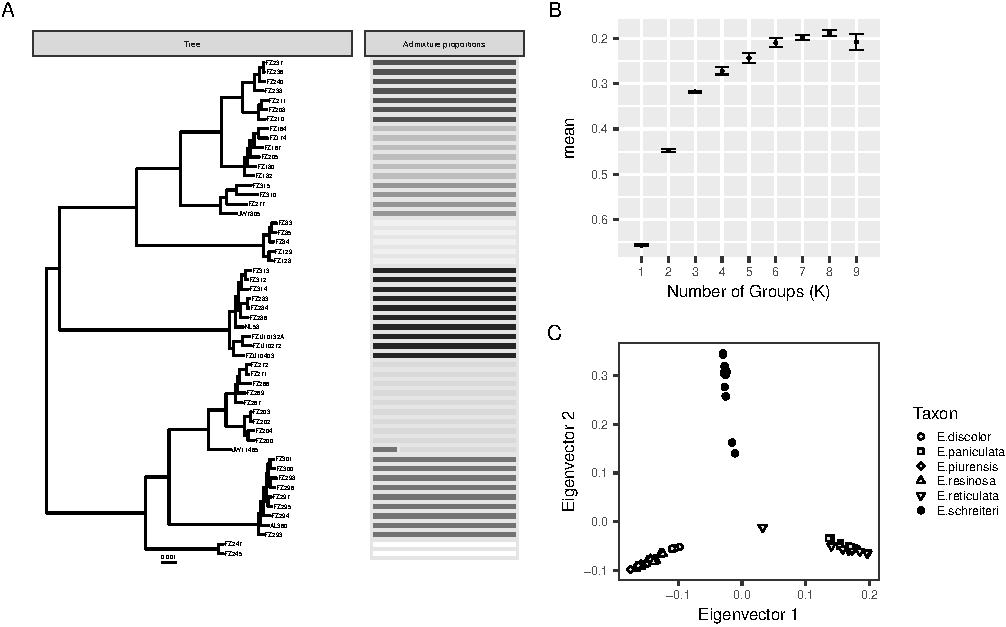
\includegraphics{Supplemental_Material_files/figure-latex/cladeIIIgenomicSensitivityAnalysesMiddleplots-1} \caption{Impact of missing data ($50\%$) on data analysis. A) maximum likelihood phylogenetic tree of specimens assigned to demes according to best \texttt{ADMIXTURE} run. B) Mean cross validation error with $95\%$ confidence interval (ordinate) for ten replicate runs of \texttt{ADMIXTURE} assuming differnt number of demes (K) (abscissa); C) Scatterplot of Principal Component Analysis (PCA) projected along the first two axes.}\label{fig:cladeIIIgenomicSensitivityAnalysesMiddleplots}
\end{figure}

Return to \protect\hyperlink{sensitivity-tests-2}{Clade III Genomics: sensitivity tests}
\pagebreak

\hypertarget{fig-s31-sensitivity-tests-with-25-missing-data}{%
\subsubsection{\texorpdfstring{Fig S31: Sensitivity tests with \(25\%\) missing data}{Fig S31: Sensitivity tests with 25\textbackslash\% missing data}}\label{fig-s31-sensitivity-tests-with-25-missing-data}}

\begin{figure}
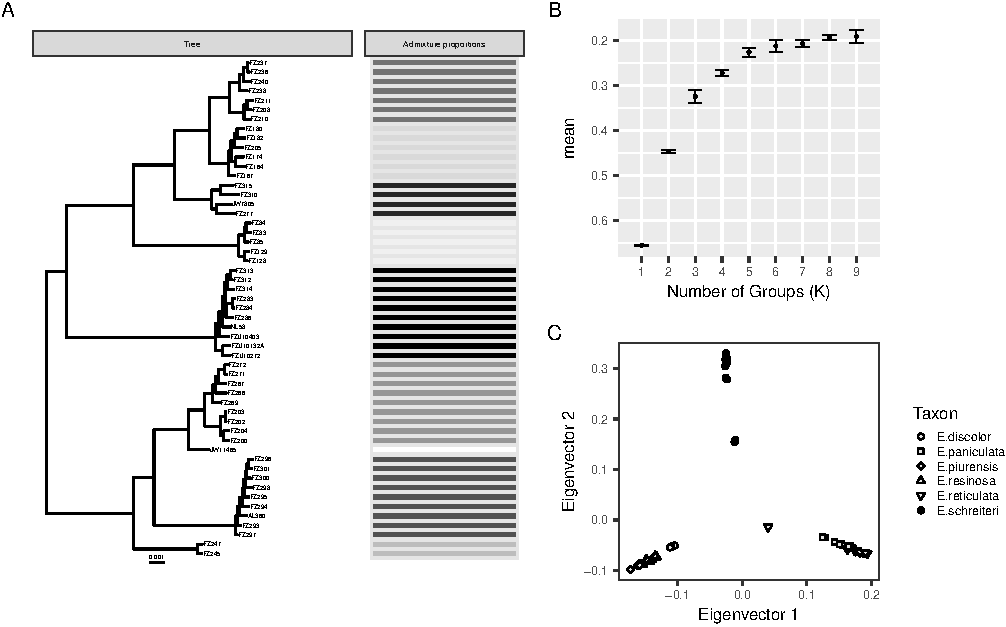
\includegraphics{Supplemental_Material_files/figure-latex/cladeIIIgenomicSensitivityAnalysesSmallestplots-1} \caption{Impact of missing data ($25\%$) on data analysis. A) maximum likelihood phylogenetic tree of specimens assigned to demes according to best \texttt{ADMIXTURE} run. B) Mean cross validation error with $95\%$ confidence interval (ordinate) for ten replicate runs of \texttt{ADMIXTURE} assuming differnt number of demes (K) (abscissa); C) Scatterplot of Principal Component Analysis (PCA) projected along the first two axes.}\label{fig:cladeIIIgenomicSensitivityAnalysesSmallestplots}
\end{figure}

Return to \protect\hyperlink{sensitivity-tests-2}{Clade III Genomics: sensitivity tests}
\pagebreak

\hypertarget{fig-s32-genogroup-delimitation-genotypic-cluster-model}{%
\subsubsection{Fig S32: Genogroup delimitation: Genotypic cluster model}\label{fig-s32-genogroup-delimitation-genotypic-cluster-model}}

\begin{figure}
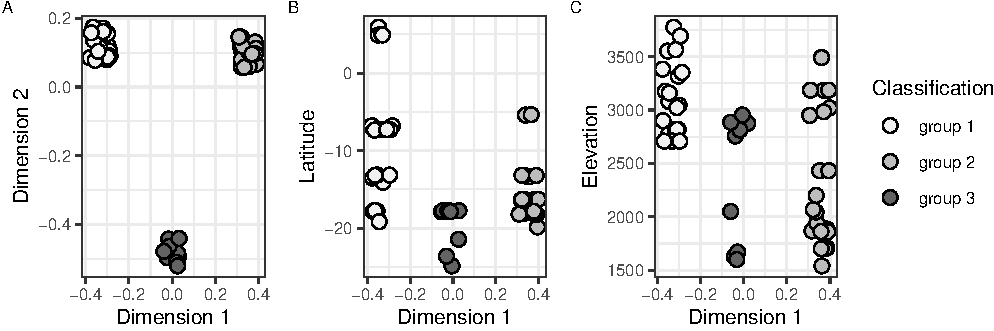
\includegraphics{Supplemental_Material_files/figure-latex/cladeIIImolecularDelimitationsNmms-1} \caption{Gaussian finite mixture modeling (GFMM) for genogroup delimitation. Visualization of the genogroups (shades) identified by the best fit Gaussian mixture model (GMM). A) genogroups in the space defined by two axes obtained by non-metric multidimensional scaling (NMDS); B) genogroups in the space defined by NMDS axis 1 and latitude; C) genogroups in the space defined by NMDS axis 1 and elevation.}\label{fig:cladeIIImolecularDelimitationsNmms}
\end{figure}

Return to \protect\hyperlink{model-based-species-discovery-5}{Clade III Genomics: model-based species discovery}
\pagebreak

\hypertarget{fig-s33-genogroup-delimitation.-cladogenesis-to-anagenesis-model}{%
\subsubsection{Fig S33: Genogroup delimitation. Cladogenesis to anagenesis model}\label{fig-s33-genogroup-delimitation.-cladogenesis-to-anagenesis-model}}

\begin{figure}
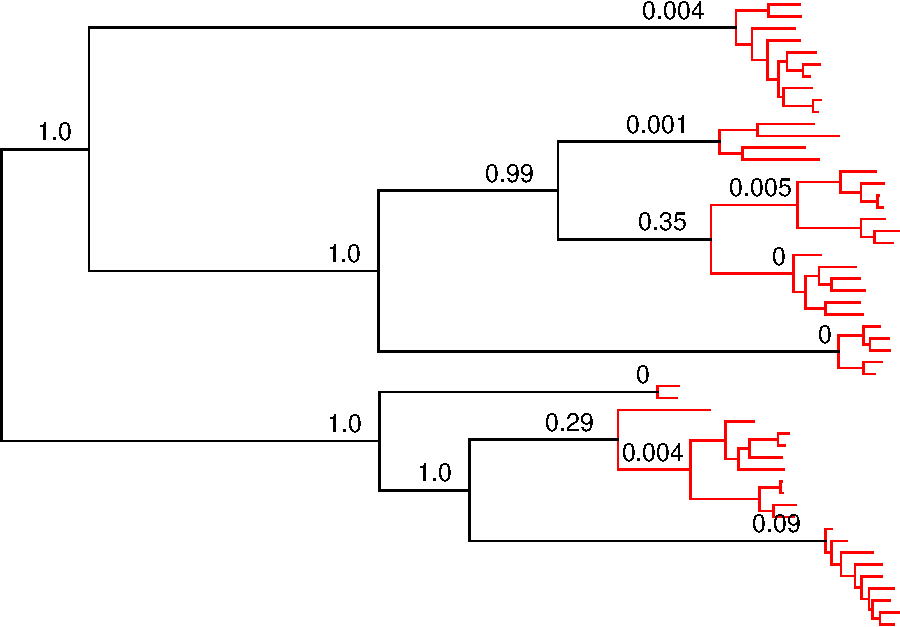
\includegraphics[height=.6\textwidth,]{Supplemental_Material_files/figure-latex/cladeIIImolecularDelimitationsPhylogeny2-1} \caption{Phylogenetic modeling for genogroup delimitation. Midpoint-rooted phylogenetic tree showing genogroups in red. Values correspond to nodes at the transition point between cladogenesis (between species) to anagenesis (within species). Values closer to 0 indicate that the node was identified as a transition to anagenesis summarized over $500$ delimitations.}\label{fig:cladeIIImolecularDelimitationsPhylogeny2}
\end{figure}

Return to \protect\hyperlink{model-based-species-discovery-5}{Clade III Genomics: model-based species discovery}
\pagebreak

\hypertarget{fig-s34-genogroup-delimitation-reproductive-isolation-model}{%
\subsubsection{Fig S34: Genogroup delimitation: Reproductive isolation model}\label{fig-s34-genogroup-delimitation-reproductive-isolation-model}}

\begin{figure}
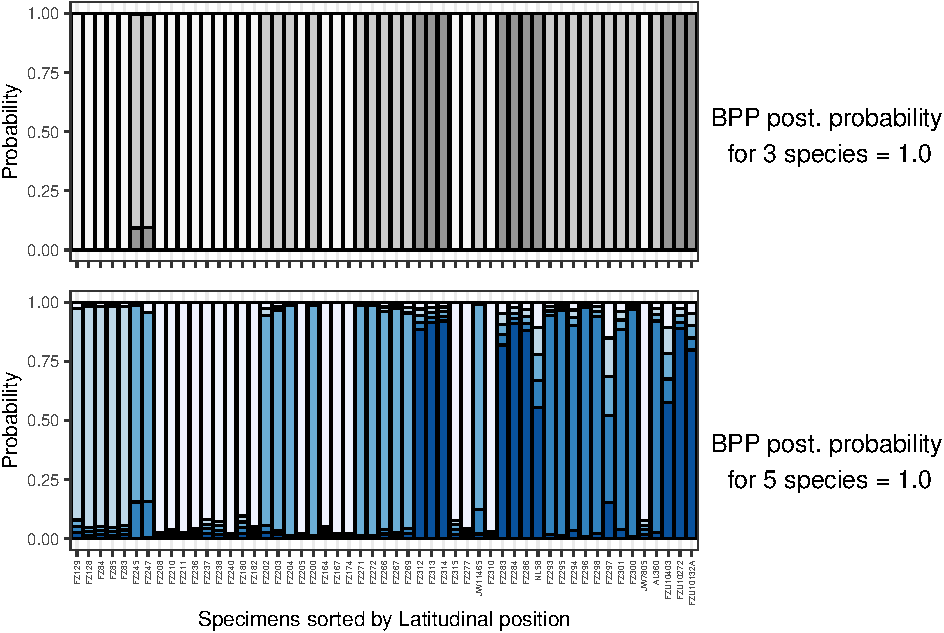
\includegraphics{Supplemental_Material_files/figure-latex/cladeIIImolecularDelimitationPopGenBpp-1} \caption{Population genetic modeling for genogroup delimitation. Top panel: assignment of specimens to demes according to \texttt{STRUCTURE} and posterior probability of species delimitation modeling according to \texttt{BPP} using these demes. Bottom panel: assignment of specimens to demes according to \texttt{MAVERICK} and posterior probability of species delimitation modeling according to \texttt{BPP} using these demes. Specimens are sorted from north (left) to south (right) according to locality of collection.}\label{fig:cladeIIImolecularDelimitationPopGenBpp}
\end{figure}

Return to \protect\hyperlink{model-based-species-discovery-5}{Clade III Genomics: model-based species discovery}
\pagebreak

\hypertarget{fig-s35-data-integration}{%
\subsubsection{Fig S35: Data integration}\label{fig-s35-data-integration}}

\begin{figure}
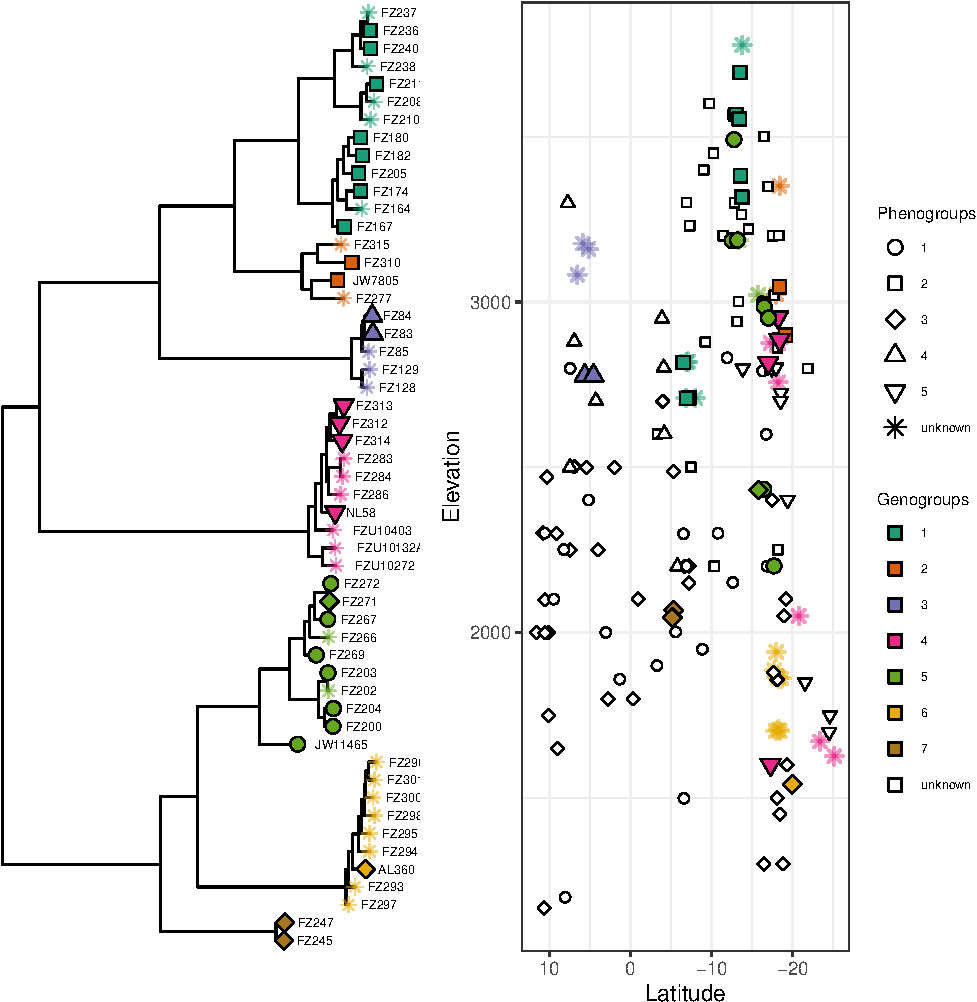
\includegraphics{Supplemental_Material_files/figure-latex/cladeIIIfinalDelimitation2-1} \caption{Integration of phenotypic and genomic data with spatial information and evolutionary history. All specimens are assigned to their corresponding best fit phenogroup (shapes) and genogroup (colors). Specimens without phenotypic or genomic data (unknown specimens) are shown as asterisks and empty shapes, accordingly. Specimens are shown as tips of the maximum likelihood tree (left) used in the CA model analysis and mapped along latitude and elevation (right). Specimens assigned to a single phenogroup and a single genogroup delineate species that we determined as 'good species'. Specimens assigned to a single phenogroup across multiple genogroups delineate species that we determined as 'phenotypic cryptic species'. Specimens assigned to a single genogroup across multiple phenogroups delineate species that we determined as 'genetic cryptic species'.}\label{fig:cladeIIIfinalDelimitation2}
\end{figure}

Return to \protect\hyperlink{data-integration-3}{Clade III Data integration}
\pagebreak

\hypertarget{clade-iv-2}{%
\subsection{Clade IV}\label{clade-iv-2}}

\hypertarget{fig-s36-taxon-sampling}{%
\subsubsection{Fig S36: Taxon sampling}\label{fig-s36-taxon-sampling}}

\begin{figure}

{\centering 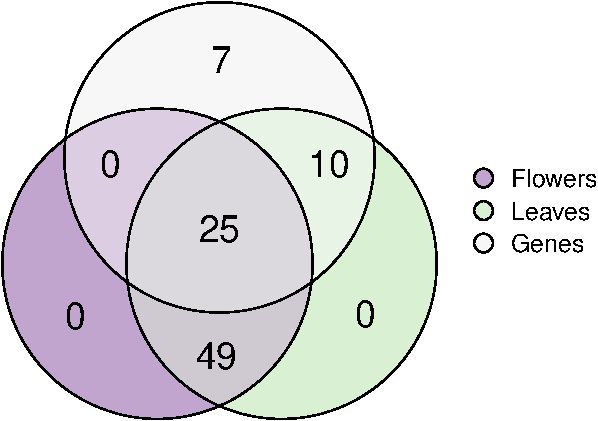
\includegraphics{Supplemental_Material_files/figure-latex/CladeIVVennDiagram-1} 

}

\caption{Specimens sampled according to three types of data. Specimens outside the Flowers category represent sterile specimens.}\label{fig:CladeIVVennDiagram}
\end{figure}

Return to \protect\hyperlink{sampling-4}{Clade IV Sampling}
\pagebreak

\hypertarget{fig-s37-geographic-distribution}{%
\subsubsection{Fig S37: Geographic distribution}\label{fig-s37-geographic-distribution}}

\begin{figure}

{\centering 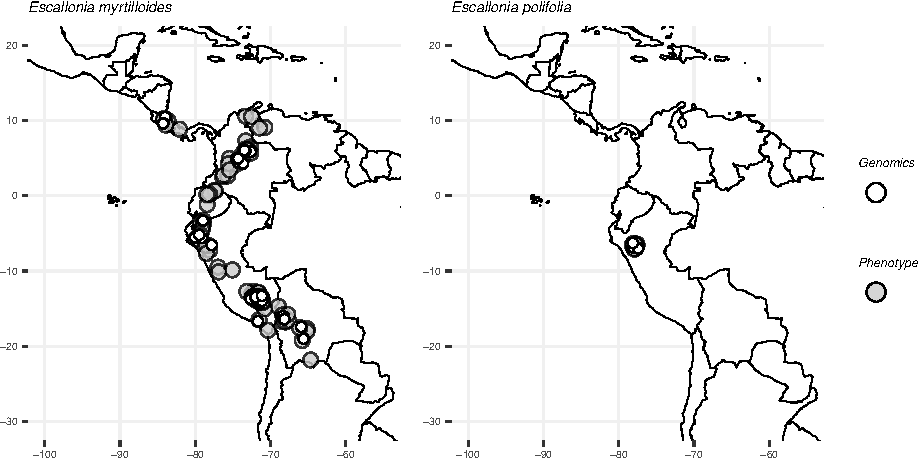
\includegraphics{Supplemental_Material_files/figure-latex/CladeIVsamplingMaps-1} 

}

\caption{Geographic distribution of specimens sampled for this clade according to taxonomic species. Filled symbols indicate specimens used in phenotypic analyses and empty symbols specimens used in genomic analyses.}\label{fig:CladeIVsamplingMaps}
\end{figure}

Return to \protect\hyperlink{sampling-4}{Clade IV Sampling}
\pagebreak

\hypertarget{fig-s38-current-state-of-taxonomic-species-with-phenotypic-data}{%
\subsubsection{Fig S38: Current state of taxonomic species with phenotypic data}\label{fig-s38-current-state-of-taxonomic-species-with-phenotypic-data}}

\begin{figure}
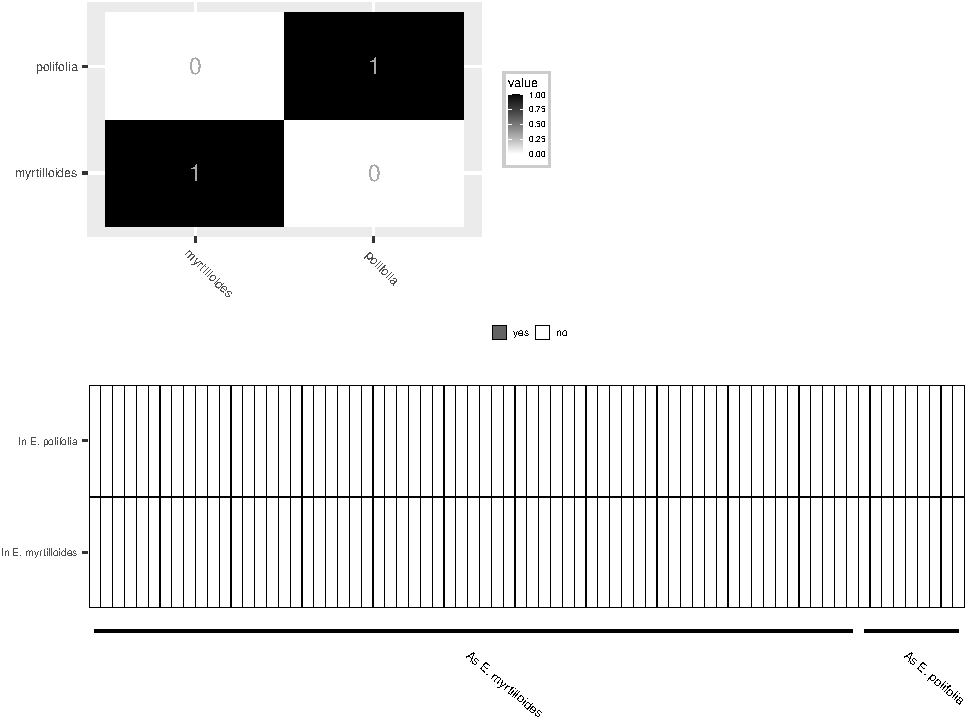
\includegraphics{Supplemental_Material_files/figure-latex/currentStateOfTaxonomyCladeIVPlots-1} \caption{Assessment of current state of taxonomic species with phenotypic data. Top panel: Pairwise overlap among 10-cubes describing geometrically each taxonomic species. Bottom panel: Matching-prediction analysis with each cell along the x-axis representing specimens sorted according to taxonomic species and the 10-cubes corresponding to each taxonomic species along the y-axis. If a specimen matches the prediction of the monograph (i.e., it is inside a 10-cube), the corresponding cell is shaded. If the specimen does not match the prediction, the cell is empty.}\label{fig:currentStateOfTaxonomyCladeIVPlots}
\end{figure}

Return to \protect\hyperlink{current-state-of-taxonomic-species-3}{Clade IV Current state of taxonomic species}
\pagebreak

\hypertarget{fig-s39-phenogroup-delimitation-gaussian-finite-mixture-modeling}{%
\subsubsection{Fig S39: Phenogroup delimitation: Gaussian finite mixture modeling}\label{fig-s39-phenogroup-delimitation-gaussian-finite-mixture-modeling}}

\begin{figure}
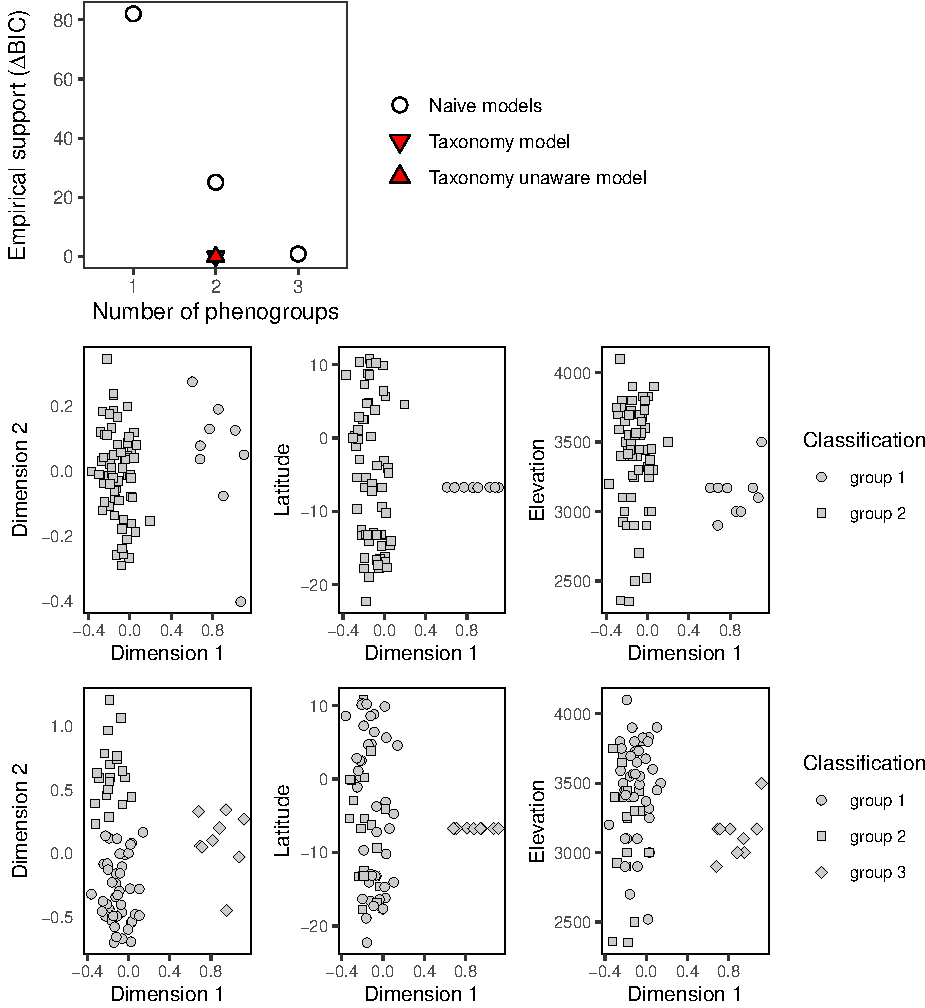
\includegraphics{Supplemental_Material_files/figure-latex/cladeIVmorphologicalDelimitationPlots-1} \caption{Gaussian finite mixture modeling (GFMM) for phenogroup delimitation and model selection using the Bayesian information criterion (BIC). Top panel: empirical support (ordinate) for Gaussian mixture models (GMM) assuming distinct number of phenogroups (abscissa). Each GMM specifies different number of phenogroups (shapes). Empirical support was measured as difference in BIC relative to the best model ($\Delta$BIC = $0$). Bottom panel: Visualization of the phenogroups (shapes) identified by the best fit GMM; left panel shows phenogroups in the space defined by two axes obtained by linear discriminat analysis (to maximize separation and visualization), middle panel shows phenogroups in the space defined by discriminant axis 1 and latitude, and right panel shows phenogroups in the space defined by discriminant axis 1 and elevation.}\label{fig:cladeIVmorphologicalDelimitationPlots}
\end{figure}

Return to \protect\hyperlink{model-based-species-discovery-6}{Clade IV Phenomics: model-based species discovery}
\pagebreak

\hypertarget{fig-s40-sensitivity-tests-with-75-missing-data}{%
\subsubsection{\texorpdfstring{Fig S40: Sensitivity tests with \(75\%\) missing data}{Fig S40: Sensitivity tests with 75\textbackslash\% missing data}}\label{fig-s40-sensitivity-tests-with-75-missing-data}}

\begin{figure}
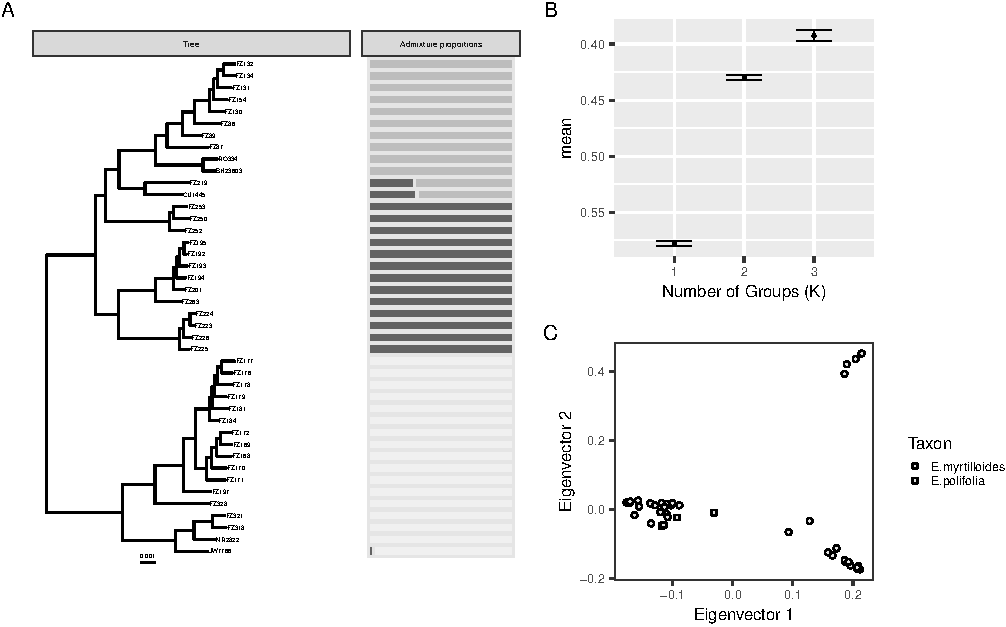
\includegraphics{Supplemental_Material_files/figure-latex/cladeIVgenomicSensitivityAnalysesLargestplots-1} \caption{Impact of missing data ($75\%$) on data analysis. A) maximum likelihood phylogenetic tree of specimens assigned to demes according to best \texttt{ADMIXTURE} run. B) Mean cross validation error with $95\%$ confidence interval (ordinate) for ten replicate runs of \texttt{ADMIXTURE} assuming differnt number of demes (K) (abscissa); C) Scatterplot of Principal Component Analysis (PCA) projected along the first two axes.}\label{fig:cladeIVgenomicSensitivityAnalysesLargestplots}
\end{figure}

Return to \protect\hyperlink{sensitivity-tests-3}{Clade IV Genomics: sensitivity tests}
\pagebreak

\hypertarget{fig-s41-sensitivity-tests-with-50-missing-data}{%
\subsubsection{\texorpdfstring{Fig S41: Sensitivity tests with \(50\%\) missing data}{Fig S41: Sensitivity tests with 50\textbackslash\% missing data}}\label{fig-s41-sensitivity-tests-with-50-missing-data}}

\begin{figure}
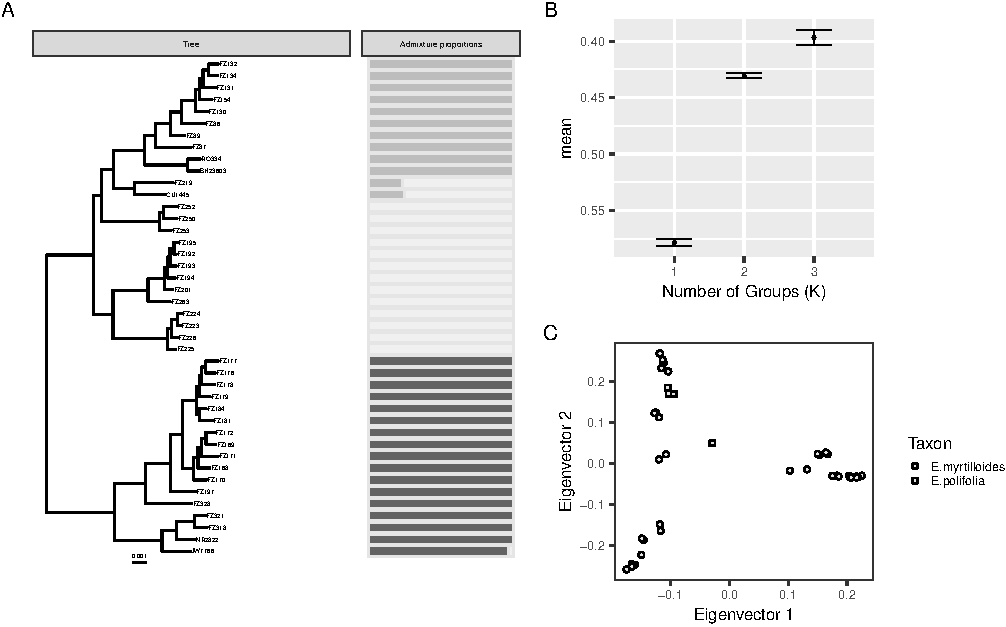
\includegraphics{Supplemental_Material_files/figure-latex/cladeIVgenomicSensitivityAnalysesMiddleplots-1} \caption{Impact of missing data ($50\%$) on data analysis. A) maximum likelihood phylogenetic tree of specimens assigned to demes according to best \texttt{ADMIXTURE} run. B) Mean cross validation error with $95\%$ confidence interval (ordinate) for ten replicate runs of \texttt{ADMIXTURE} assuming differnt number of demes (K) (abscissa); C) Scatterplot of Principal Component Analysis (PCA) projected along the first two axes.}\label{fig:cladeIVgenomicSensitivityAnalysesMiddleplots}
\end{figure}

Return to \protect\hyperlink{sensitivity-tests-3}{Clade IV Genomics: sensitivity tests}
\pagebreak

\hypertarget{fig-s42-sensitivity-tests-with-25-missing-data}{%
\subsubsection{\texorpdfstring{Fig S42: Sensitivity tests with \(25\%\) missing data}{Fig S42: Sensitivity tests with 25\textbackslash\% missing data}}\label{fig-s42-sensitivity-tests-with-25-missing-data}}

\begin{figure}
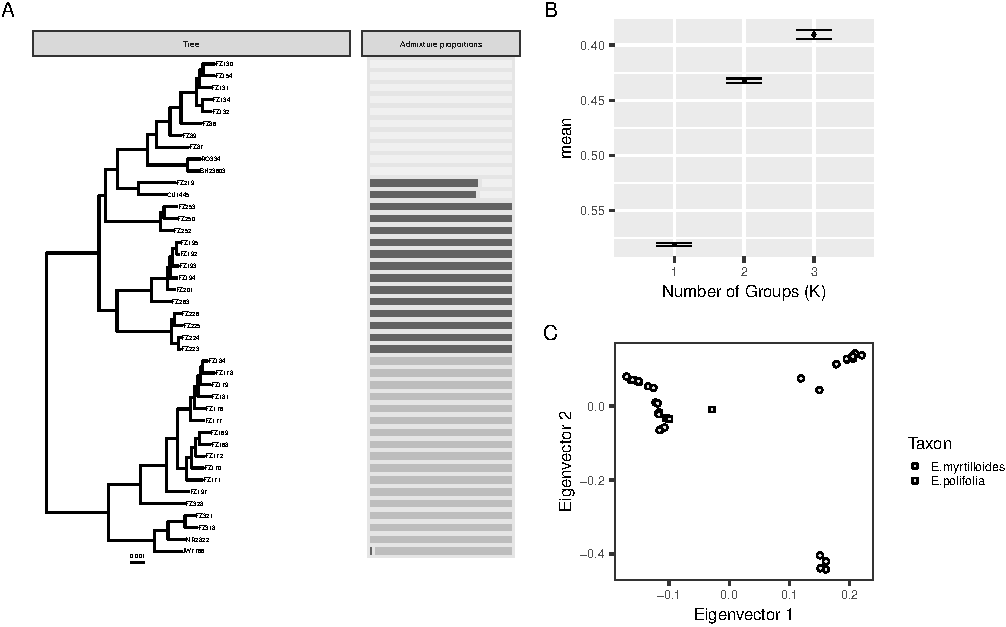
\includegraphics{Supplemental_Material_files/figure-latex/cladeIVgenomicSensitivityAnalysesSmallestplots-1} \caption{Impact of missing data ($25\%$) on data analysis. A) maximum likelihood phylogenetic tree of specimens assigned to demes according to best \texttt{ADMIXTURE} run. B) Mean cross validation error with $95\%$ confidence interval (ordinate) for ten replicate runs of \texttt{ADMIXTURE} assuming differnt number of demes (K) (abscissa); C) Scatterplot of Principal Component Analysis (PCA) projected along the first two axes.}\label{fig:cladeIVgenomicSensitivityAnalysesSmallestplots}
\end{figure}

Return to \protect\hyperlink{sensitivity-tests-3}{Clade IV Genomics: sensitivity tests}
\pagebreak

\hypertarget{fig-s43-genogroup-delimitation-genotypic-cluster-model}{%
\subsubsection{Fig S43: Genogroup delimitation: Genotypic cluster model}\label{fig-s43-genogroup-delimitation-genotypic-cluster-model}}

\begin{figure}
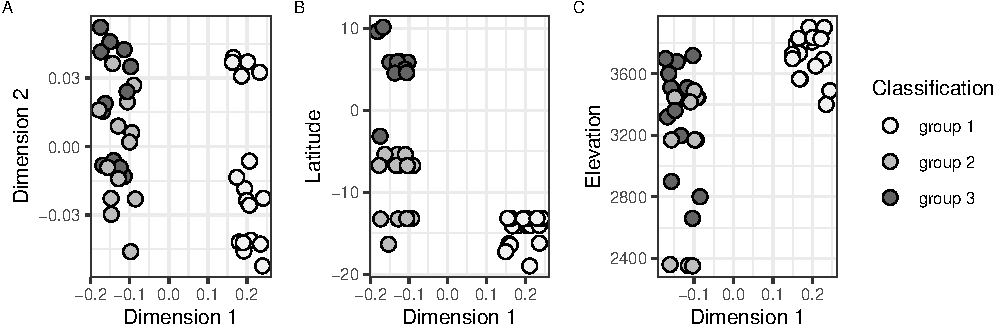
\includegraphics{Supplemental_Material_files/figure-latex/cladeIVmolecularDelimitationsNmms-1} \caption{Gaussian finite mixture modeling (GFMM) for genogroup delimitation. Visualization of the genogroups (shades) identified by the best fit Gaussian mixture model (GMM). A) genogroups in the space defined by two axes obtained by non-metric multidimensional scaling (NMDS); B) genogroups in the space defined by NMDS axis 1 and latitude; C) genogroups in the space defined by NMDS axis 1 and elevation.}\label{fig:cladeIVmolecularDelimitationsNmms}
\end{figure}

Return to \protect\hyperlink{model-based-species-discovery-7}{Clade IV Genomics: model-based species discovery}
\pagebreak

\hypertarget{fig-s44-genogroup-delimitation.-cladogenesis-to-anagenesis-model}{%
\subsubsection{Fig S44: Genogroup delimitation. Cladogenesis to anagenesis model}\label{fig-s44-genogroup-delimitation.-cladogenesis-to-anagenesis-model}}

\begin{figure}
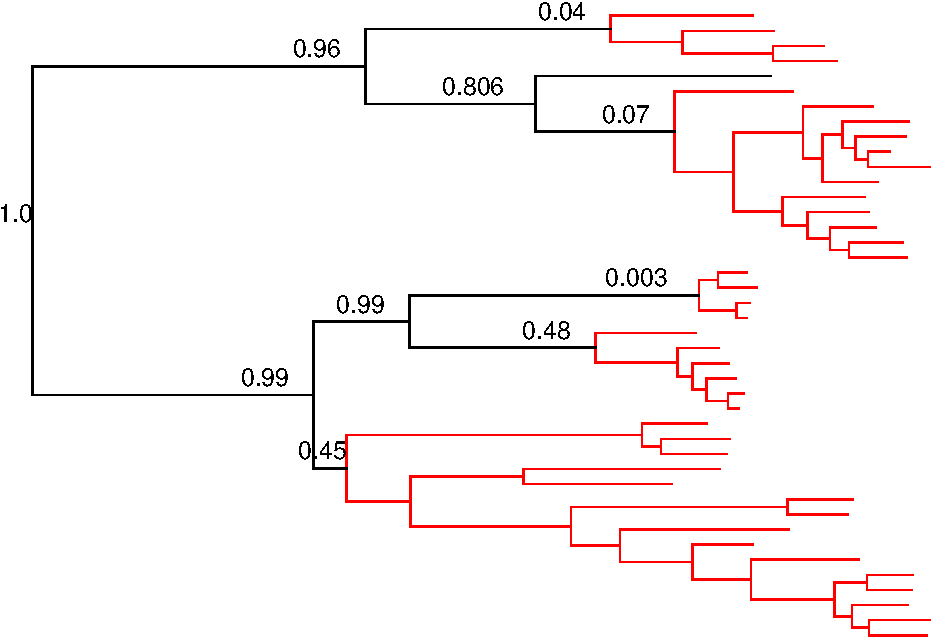
\includegraphics[height=.6\textwidth,]{Supplemental_Material_files/figure-latex/cladeIVmolecularDelimitationsPhylogeny2-1} \caption{Phylogenetic modeling for genogroup delimitation. Midpoint-rooted phylogenetic tree showing genogroups in red. Values correspond to nodes at the transition point between cladogenesis (between species) to anagenesis (within species). Values closer to 0 indicate that the node was identified as a transition to anagenesis summarized over $500$ delimitations.}\label{fig:cladeIVmolecularDelimitationsPhylogeny2}
\end{figure}

Return to \protect\hyperlink{model-based-species-discovery-7}{Clade IV Genomics: model-based species discovery}
\pagebreak

\hypertarget{fig-s45-genogroup-delimitation-reproductive-isolation-model}{%
\subsubsection{Fig S45: Genogroup delimitation: Reproductive isolation model}\label{fig-s45-genogroup-delimitation-reproductive-isolation-model}}

\begin{figure}
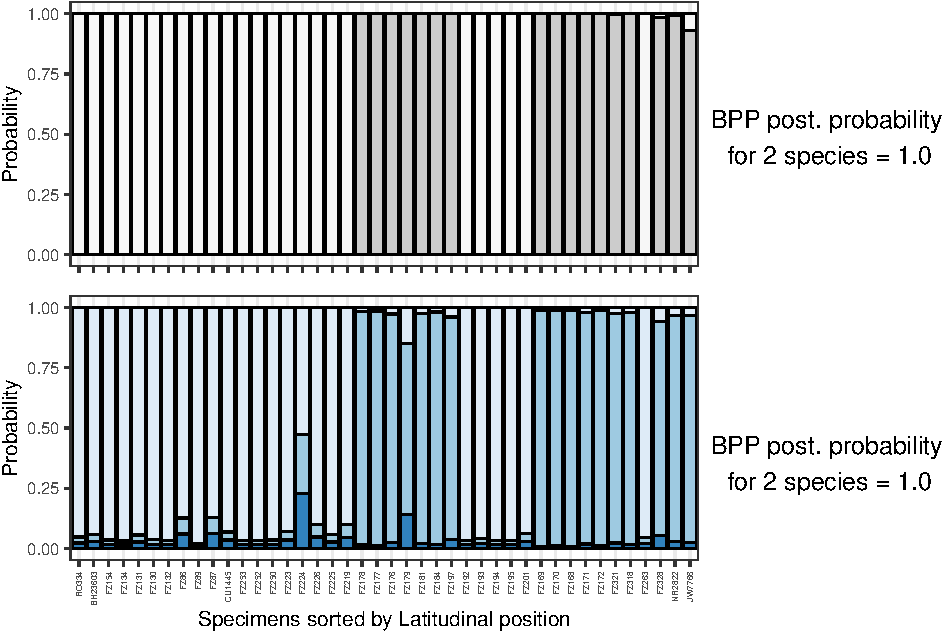
\includegraphics{Supplemental_Material_files/figure-latex/cladeIVmolecularDelimitationPopGenBpp-1} \caption{Population genetic modeling for genogroup delimitation. Top panel: assignment of specimens to demes according to \texttt{STRUCTURE} and posterior probability of species delimitation modeling according to \texttt{BPP} using these demes. Bottom panel: assignment of specimens to demes according to \texttt{MAVERICK} and posterior probability of species delimitation modeling according to \texttt{BPP} using these demes. Specimens are sorted from north (left) to south (right) according to locality of collection.}\label{fig:cladeIVmolecularDelimitationPopGenBpp}
\end{figure}

Return to \protect\hyperlink{model-based-species-discovery-7}{Clade IV Genomics: model-based species discovery}
\pagebreak

\hypertarget{fig-s46-data-integration}{%
\subsubsection{Fig S46: Data integration}\label{fig-s46-data-integration}}

\begin{figure}
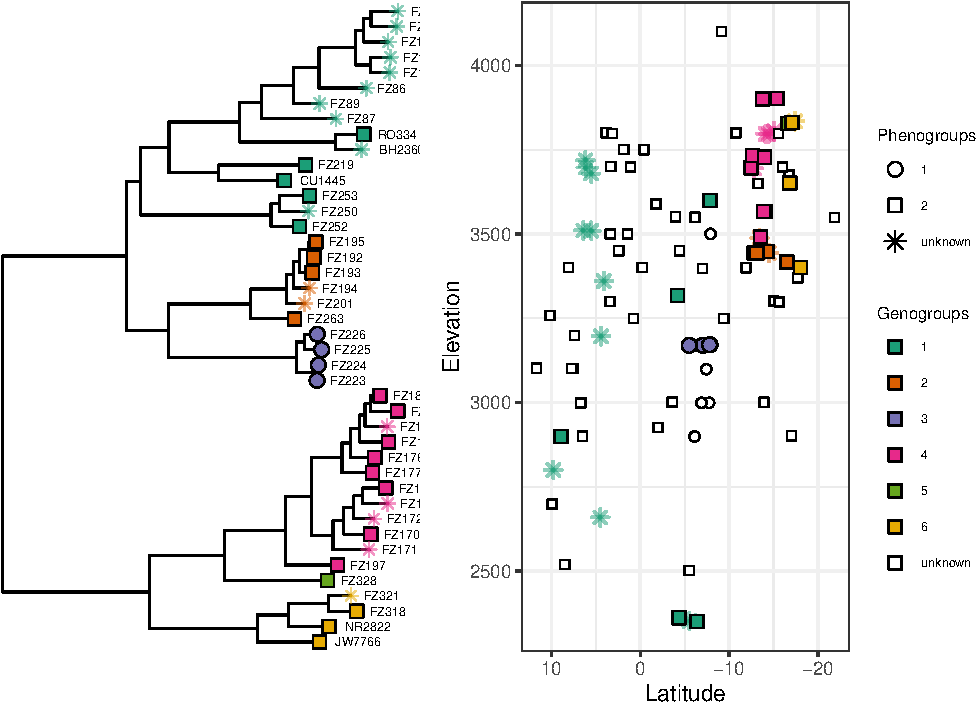
\includegraphics{Supplemental_Material_files/figure-latex/cladeIVfinalDelimitation2-1} \caption{Integration of phenotypic and genomic data with spatial information and evolutionary history. All specimens are assigned to their corresponding best fit phenogroup (shapes) and genogroup (colors). Specimens without phenotypic or genomic data (unknown specimens) are shown as asterisks and empty shapes, accordingly. Specimens are shown as tips of the maximum likelihood tree (left) used in the CA model analysis and mapped along latitude and elevation (right). Specimens assigned to a single phenogroup and a single genogroup delineate species that we determined as 'good species'. Specimens assigned to a single phenogroup across multiple genogroups delineate species that we determined as 'phenotypic cryptic species'. Specimens assigned to a single genogroup across multiple phenogroups delineate species that we determined as 'genetic cryptic species'.}\label{fig:cladeIVfinalDelimitation2}
\end{figure}

Return to \protect\hyperlink{data-integration-4}{Clade IV Data integration}
\pagebreak

\hypertarget{clade-v-2}{%
\subsection{Clade V}\label{clade-v-2}}

\hypertarget{fig-s47-taxon-sampling}{%
\subsubsection{Fig S47: Taxon sampling}\label{fig-s47-taxon-sampling}}

\begin{figure}

{\centering 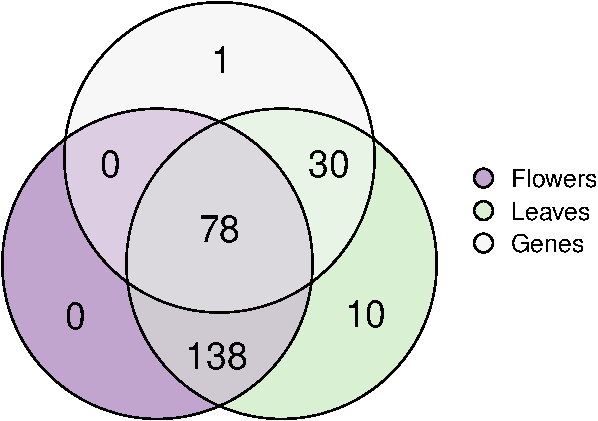
\includegraphics{Supplemental_Material_files/figure-latex/CladeVVennDiagram-1} 

}

\caption{Specimens sampled according to three types of data. Specimens outside the Flowers category represent sterile specimens.}\label{fig:CladeVVennDiagram}
\end{figure}

Return to \protect\hyperlink{sampling-5}{Clade V Sampling}
\pagebreak

\hypertarget{fig-s48-geographic-distribution}{%
\subsubsection{Fig S48: Geographic distribution}\label{fig-s48-geographic-distribution}}

\begin{figure}

{\centering 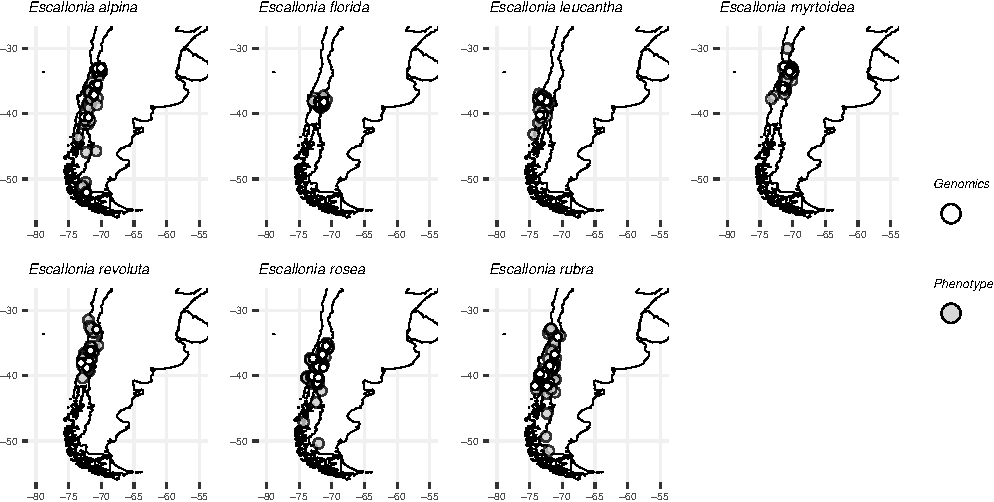
\includegraphics{Supplemental_Material_files/figure-latex/CladeVsamplingMaps-1} 

}

\caption{Geographic distribution of specimens sampled for this clade according to taxonomic species. Filled symbols indicate specimens used in phenotypic analyses and empty symbols specimens used in genomic analyses.}\label{fig:CladeVsamplingMaps}
\end{figure}

Return to \protect\hyperlink{sampling-5}{Clade V Sampling}
\pagebreak

\pagebreak

\hypertarget{fig-s49-current-state-of-taxonomic-species-with-phenotypic-data}{%
\subsubsection{Fig S49: Current state of taxonomic species with phenotypic data}\label{fig-s49-current-state-of-taxonomic-species-with-phenotypic-data}}

\begin{figure}
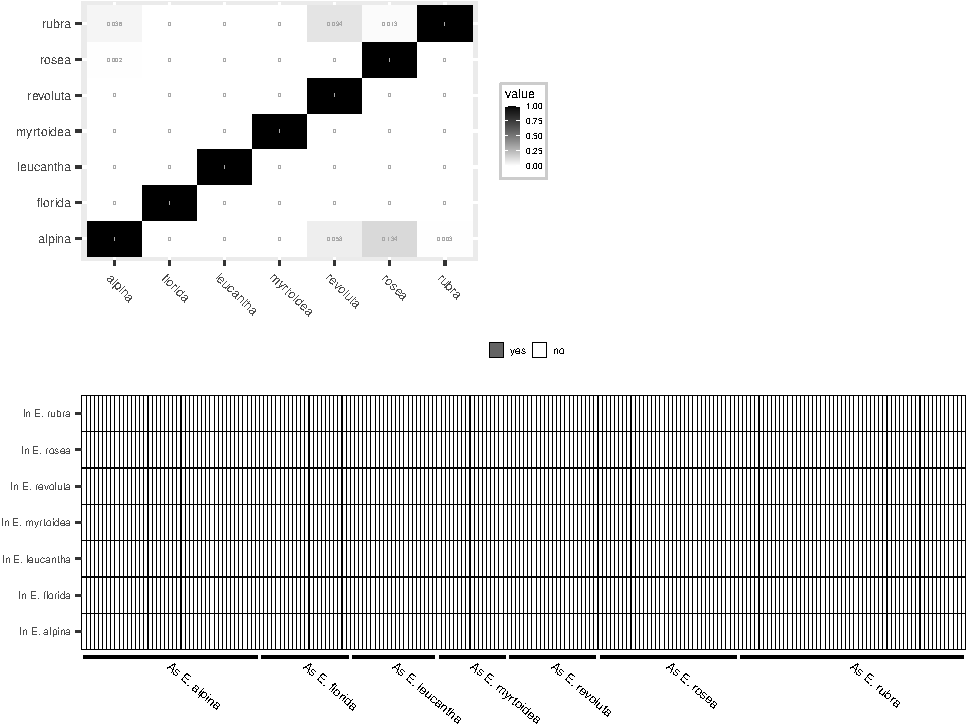
\includegraphics{Supplemental_Material_files/figure-latex/currentStateOfTaxonomyCladeVPlots-1} \caption{Assessment of current state of taxonomic species with phenotypic data. Top panel: Pairwise overlap among 10-cubes describing geometrically each taxonomic species. Bottom panel: Matching-prediction analysis with each cell along the x-axis representing specimens sorted according to taxonomic species and the 10-cubes corresponding to each taxonomic species along the y-axis. If a specimen matches the prediction of the monograph (i.e., it is inside a 10-cube), the corresponding cell is shaded. If the specimen does not match the prediction, the cell is empty.}\label{fig:currentStateOfTaxonomyCladeVPlots}
\end{figure}

Return to \protect\hyperlink{current-state-of-taxonomic-species-4}{Clade V Current state of taxonomic species}
\pagebreak

\hypertarget{fig-s50-phenogroup-delimitation-gaussian-finite-mixture-modeling}{%
\subsubsection{Fig S50: Phenogroup delimitation: Gaussian finite mixture modeling}\label{fig-s50-phenogroup-delimitation-gaussian-finite-mixture-modeling}}

\begin{figure}
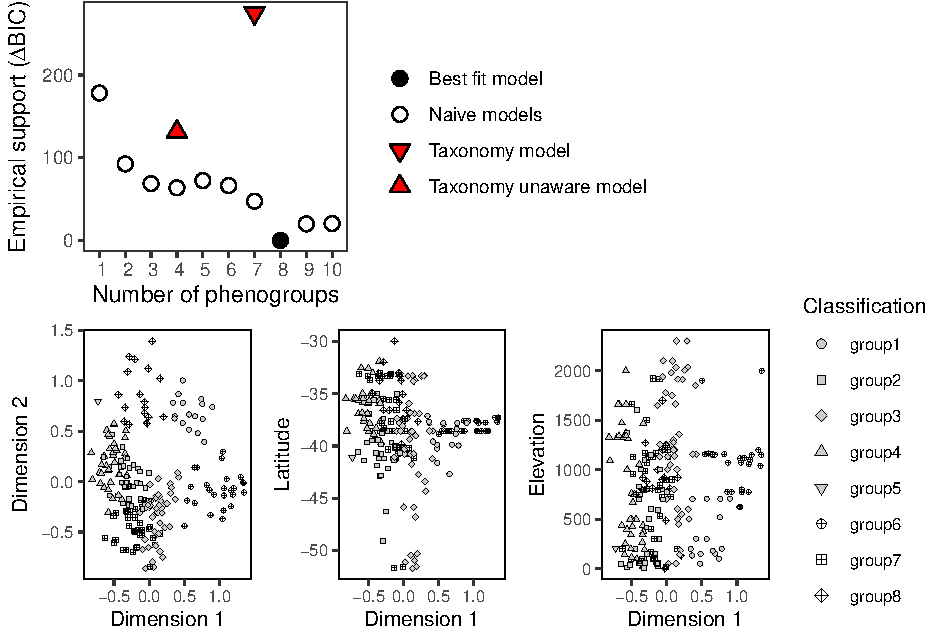
\includegraphics{Supplemental_Material_files/figure-latex/cladeVmorphologicalDelimitationPlots-1} \caption{Gaussian finite mixture modeling (GFMM) for phenogroup delimitation and model selection using the Bayesian information criterion (BIC). Top panel: empirical support (ordinate) for Gaussian mixture models (GMM) assuming distinct number of phenogroups (abscissa). Each GMM specifies different number of phenogroups (shapes). Empirical support was measured as difference in BIC relative to the best model ($\Delta$BIC = $0$). Bottom panel: Visualization of the phenogroups (shapes) identified by the best fit GMM; left panel shows phenogroups in the space defined by two axes obtained by linear discriminat analysis (to maximize separation and visualization), middle panel shows phenogroups in the space defined by discriminant axis 1 and latitude, and right panel shows phenogroups in the space defined by discriminant axis 1 and elevation.}\label{fig:cladeVmorphologicalDelimitationPlots}
\end{figure}

Return to \protect\hyperlink{model-based-species-discovery-8}{Clade V Phenomics: model-based species discovery}
\pagebreak

\hypertarget{fig-s51-sensitivity-tests-with-75-missing-data}{%
\subsubsection{\texorpdfstring{Fig S51: Sensitivity tests with \(75\%\) missing data}{Fig S51: Sensitivity tests with 75\textbackslash\% missing data}}\label{fig-s51-sensitivity-tests-with-75-missing-data}}

\begin{figure}
\includegraphics{Supplemental_Material_files/figure-latex/cladeVgenomicSensitivityAnalysesLargestplots-1} \caption{Impact of missing data ($75\%$) on data analysis. A) maximum likelihood phylogenetic tree of specimens assigned to demes according to best \texttt{ADMIXTURE} run. B) Mean cross validation error with $95\%$ confidence interval (ordinate) for ten replicate runs of \texttt{ADMIXTURE} assuming differnt number of demes (K) (abscissa); C) Scatterplot of Principal Component Analysis (PCA) projected along the first two axes.}\label{fig:cladeVgenomicSensitivityAnalysesLargestplots}
\end{figure}

Return to \protect\hyperlink{sensitivity-tests-4}{Clade V Genomics: sensitivity tests}
\pagebreak

\hypertarget{fig-s52-sensitivity-tests-with-50-missing-data}{%
\subsubsection{\texorpdfstring{Fig S52: Sensitivity tests with \(50\%\) missing data}{Fig S52: Sensitivity tests with 50\textbackslash\% missing data}}\label{fig-s52-sensitivity-tests-with-50-missing-data}}

\begin{figure}
\includegraphics{Supplemental_Material_files/figure-latex/cladeVgenomicSensitivityAnalysesMiddleplots-1} \caption{Impact of missing data ($50\%$) on data analysis. A) maximum likelihood phylogenetic tree of specimens assigned to demes according to best \texttt{ADMIXTURE} run. B) Mean cross validation error with $95\%$ confidence interval (ordinate) for ten replicate runs of \texttt{ADMIXTURE} assuming differnt number of demes (K) (abscissa); C) Scatterplot of Principal Component Analysis (PCA) projected along the first two axes.}\label{fig:cladeVgenomicSensitivityAnalysesMiddleplots}
\end{figure}

Return to \protect\hyperlink{sensitivity-tests-4}{Clade V Genomics: sensitivity tests}
\pagebreak

\hypertarget{fig-s53-sensitivity-tests-with-25-missing-data}{%
\subsubsection{\texorpdfstring{Fig S53: Sensitivity tests with \(25\%\) missing data}{Fig S53: Sensitivity tests with 25\textbackslash\% missing data}}\label{fig-s53-sensitivity-tests-with-25-missing-data}}

\begin{figure}
\includegraphics{Supplemental_Material_files/figure-latex/cladeVgenomicSensitivityAnalysesSmallestplots-1} \caption{Impact of missing data ($25\%$) on data analysis. A) maximum likelihood phylogenetic tree of specimens assigned to demes according to best \texttt{ADMIXTURE} run. B) Mean cross validation error with $95\%$ confidence interval (ordinate) for ten replicate runs of \texttt{ADMIXTURE} assuming differnt number of demes (K) (abscissa); C) Scatterplot of Principal Component Analysis (PCA) projected along the first two axes.}\label{fig:cladeVgenomicSensitivityAnalysesSmallestplots}
\end{figure}

Return to \protect\hyperlink{sensitivity-tests-4}{Clade V Genomics: sensitivity tests}
\pagebreak

\hypertarget{fig-s54-genogroup-delimitation-genotypic-cluster-model}{%
\subsubsection{Fig S54: Genogroup delimitation: Genotypic cluster model}\label{fig-s54-genogroup-delimitation-genotypic-cluster-model}}

\begin{figure}
\includegraphics{Supplemental_Material_files/figure-latex/cladeVmolecularDelimitationsNmms-1} \caption{Gaussian finite mixture modeling (GFMM) for genogroup delimitation. Visualization of the genogroups (shades) identified by the best fit Gaussian mixture model (GMM). A) genogroups in the space defined by two axes obtained by non-metric multidimensional scaling (NMDS); B) genogroups in the space defined by NMDS axis 1 and latitude; C) genogroups in the space defined by NMDS axis 1 and elevation.}\label{fig:cladeVmolecularDelimitationsNmms}
\end{figure}

Return to \protect\hyperlink{model-based-species-discovery-9}{Clade V Genomics: model-based species discovery}
\pagebreak

\hypertarget{fig-s55-genogroup-delimitation.-cladogenesis-to-anagenesis-model}{%
\subsubsection{Fig S55: Genogroup delimitation. Cladogenesis to anagenesis model}\label{fig-s55-genogroup-delimitation.-cladogenesis-to-anagenesis-model}}

\begin{figure}
\includegraphics[height=.6\textwidth,]{Supplemental_Material_files/figure-latex/cladeVmolecularDelimitationsPhylogeny2-1} \caption{Phylogenetic modeling for genogroup delimitation. Midpoint-rooted phylogenetic tree showing genogroups in red. Values correspond to nodes at the transition point between cladogenesis (between species) to anagenesis (within species). Values closer to 0 indicate that the node was identified as a transition to anagenesis summarized over $500$ delimitations.}\label{fig:cladeVmolecularDelimitationsPhylogeny2}
\end{figure}

Return to \protect\hyperlink{model-based-species-discovery-9}{Clade V Genomics: model-based species discovery}
\pagebreak

\hypertarget{fig-s56-genogroup-delimitation-reproductive-isolation-model}{%
\subsubsection{Fig S56: Genogroup delimitation: Reproductive isolation model}\label{fig-s56-genogroup-delimitation-reproductive-isolation-model}}

\begin{figure}
\includegraphics{Supplemental_Material_files/figure-latex/cladeVmolecularDelimitationPopGenBpp-1} \caption{Population genetic modeling for genogroup delimitation. Top panel: assignment of specimens to demes according to \texttt{STRUCTURE} and posterior probability of species delimitation modeling according to \texttt{BPP} using these demes. Bottom panel: assignment of specimens to demes according to \texttt{MAVERICK} and posterior probability of species delimitation modeling according to \texttt{BPP} using these demes. Specimens are sorted from north (left) to south (right) according to locality of collection.}\label{fig:cladeVmolecularDelimitationPopGenBpp}
\end{figure}

Return to \protect\hyperlink{model-based-species-discovery-9}{Clade V Genomics: model-based species discovery}
\pagebreak

\hypertarget{fig-s57-data-integration}{%
\subsubsection{Fig S57: Data integration}\label{fig-s57-data-integration}}

\begin{figure}
\includegraphics{Supplemental_Material_files/figure-latex/cladeVfinalDelimitation2-1} \caption{Integration of phenotypic and genomic data with spatial information and evolutionary history. All specimens are assigned to their corresponding best fit phenogroup (shapes) and genogroup (colors). Specimens without phenotypic or genomic data (unknown specimens) are shown as asterisks and empty shapes, accordingly. Specimens are shown as tips of the maximum likelihood tree (left) used in the CA model analysis and mapped along latitude and elevation (right). Specimens assigned to a single phenogroup and a single genogroup delineate species that we determined as 'good species'. Specimens assigned to a single phenogroup across multiple genogroups delineate species that we determined as 'phenotypic cryptic species'. Specimens assigned to a single genogroup across multiple phenogroups delineate species that we determined as 'genetic cryptic species'.}\label{fig:cladeVfinalDelimitation2}
\end{figure}

Return to \protect\hyperlink{data-integration-5}{Clade V Data integration}
\pagebreak

\hypertarget{clade-vi-2}{%
\subsection{Clade VI}\label{clade-vi-2}}

\hypertarget{fig-s58-taxon-sampling}{%
\subsubsection{Fig S58: Taxon sampling}\label{fig-s58-taxon-sampling}}

\begin{figure}

{\centering \includegraphics{Supplemental_Material_files/figure-latex/CladeVIVennDiagram-1} 

}

\caption{Specimens sampled according to three types of data. Specimens outside the Flowers category represent sterile specimens.}\label{fig:CladeVIVennDiagram}
\end{figure}

Return to \protect\hyperlink{sampling-6}{Clade VI Sampling}
\pagebreak

\hypertarget{fig-s59-geographic-distribution}{%
\subsubsection{Fig S59: Geographic distribution}\label{fig-s59-geographic-distribution}}

\begin{figure}

{\centering \includegraphics{Supplemental_Material_files/figure-latex/CladeVIsamplingMaps-1} 

}

\caption{Geographic distribution of specimens sampled for this clade according to taxonomic species. Filled symbols indicate specimens used in phenotypic analyses and empty symbols specimens used in genomic analyses.}\label{fig:CladeVIsamplingMaps}
\end{figure}

Return to \protect\hyperlink{sampling-6}{Clade VI Sampling}
\pagebreak

\hypertarget{fig-s60-current-state-of-taxonomic-species-with-phenotypic-data}{%
\subsubsection{Fig S60: Current state of taxonomic species with phenotypic data}\label{fig-s60-current-state-of-taxonomic-species-with-phenotypic-data}}

\begin{figure}
\includegraphics{Supplemental_Material_files/figure-latex/currentStateOfTaxonomyCladeVIPlots-1} \caption{Assessment of current state of taxonomic species with phenotypic data. Top panel: Pairwise overlap among 10-cubes describing geometrically each taxonomic species. Bottom panel: Matching-prediction analysis with each cell along the x-axis representing specimens sorted according to taxonomic species and the 10-cubes corresponding to each taxonomic species along the y-axis. If a specimen matches the prediction of the monograph (i.e., it is inside a 10-cube), the corresponding cell is shaded. If the specimen does not match the prediction, the cell is empty.}\label{fig:currentStateOfTaxonomyCladeVIPlots}
\end{figure}

Return to \protect\hyperlink{current-state-of-taxonomic-species-5}{Clade VI Current state of taxonomic species}
\pagebreak

\hypertarget{fig-s61-phenogroup-delimitation-gaussian-finite-mixture-modeling}{%
\subsubsection{Fig S61: Phenogroup delimitation: Gaussian finite mixture modeling}\label{fig-s61-phenogroup-delimitation-gaussian-finite-mixture-modeling}}

\begin{figure}
\includegraphics{Supplemental_Material_files/figure-latex/cladeVImorphologicalDelimitationPlots-1} \caption{Gaussian finite mixture modeling (GFMM) for phenogroup delimitation and model selection using the Bayesian information criterion (BIC). Top panel: empirical support (ordinate) for Gaussian mixture models (GMM) assuming distinct number of phenogroups (abscissa). Each GMM specifies different number of phenogroups (shapes). Empirical support was measured as difference in BIC relative to the best model ($\Delta$BIC = $0$). Bottom panel: Visualization of the phenogroups (shapes) identified by the best fit GMM; left panel shows phenogroups in the space defined by two axes obtained by linear discriminat analysis (to maximize separation and visualization), middle panel shows phenogroups in the space defined by discriminant axis 1 and latitude, and right panel shows phenogroups in the space defined by discriminant axis 1 and elevation.}\label{fig:cladeVImorphologicalDelimitationPlots}
\end{figure}

Return to \protect\hyperlink{model-based-species-discovery-10}{Clade VI Phenomics: model-based species discovery}
\pagebreak

\hypertarget{fig-s62-sensitivity-tests-with-75-missing-data}{%
\subsubsection{\texorpdfstring{Fig S62: Sensitivity tests with \(75\%\) missing data}{Fig S62: Sensitivity tests with 75\textbackslash\% missing data}}\label{fig-s62-sensitivity-tests-with-75-missing-data}}

\begin{figure}
\includegraphics{Supplemental_Material_files/figure-latex/cladeVIgenomicSensitivityAnalysesLargestplots-1} \caption{Impact of missing data ($75\%$) on data analysis. A) maximum likelihood phylogenetic tree of specimens assigned to demes according to best \texttt{ADMIXTURE} run. B) Mean cross validation error with $95\%$ confidence interval (ordinate) for ten replicate runs of \texttt{ADMIXTURE} assuming differnt number of demes (K) (abscissa); C) Scatterplot of Principal Component Analysis (PCA) projected along the first two axes.}\label{fig:cladeVIgenomicSensitivityAnalysesLargestplots}
\end{figure}

Return to \protect\hyperlink{sensitivity-tests-5}{Clade VI Genomics: sensitivity tests}
\pagebreak

\hypertarget{fig-s63-sensitivity-tests-with-50-missing-data}{%
\subsubsection{\texorpdfstring{Fig S63: Sensitivity tests with \(50\%\) missing data}{Fig S63: Sensitivity tests with 50\textbackslash\% missing data}}\label{fig-s63-sensitivity-tests-with-50-missing-data}}

\begin{figure}
\includegraphics{Supplemental_Material_files/figure-latex/cladeVIgenomicSensitivityAnalysesMiddleplots-1} \caption{Impact of missing data ($50\%$) on data analysis. A) maximum likelihood phylogenetic tree of specimens assigned to demes according to best \texttt{ADMIXTURE} run. B) Mean cross validation error with $95\%$ confidence interval (ordinate) for ten replicate runs of \texttt{ADMIXTURE} assuming differnt number of demes (K) (abscissa); C) Scatterplot of Principal Component Analysis (PCA) projected along the first two axes.}\label{fig:cladeVIgenomicSensitivityAnalysesMiddleplots}
\end{figure}

Return to \protect\hyperlink{sensitivity-tests-5}{Clade VI Genomics: sensitivity tests}
\pagebreak

\hypertarget{fig-s64-sensitivity-tests-with-25-missing-data}{%
\subsubsection{\texorpdfstring{Fig S64: Sensitivity tests with \(25\%\) missing data}{Fig S64: Sensitivity tests with 25\textbackslash\% missing data}}\label{fig-s64-sensitivity-tests-with-25-missing-data}}

\begin{figure}
\includegraphics{Supplemental_Material_files/figure-latex/cladeVIgenomicSensitivityAnalysesSmallestplots-1} \caption{Impact of missing data ($25\%$) on data analysis. A) maximum likelihood phylogenetic tree of specimens assigned to demes according to best \texttt{ADMIXTURE} run. B) Mean cross validation error with $95\%$ confidence interval (ordinate) for ten replicate runs of \texttt{ADMIXTURE} assuming differnt number of demes (K) (abscissa); C) Scatterplot of Principal Component Analysis (PCA) projected along the first two axes.}\label{fig:cladeVIgenomicSensitivityAnalysesSmallestplots}
\end{figure}

Return to \protect\hyperlink{sensitivity-tests-5}{Clade VI Genomics: sensitivity tests}
\pagebreak

\hypertarget{fig-s65-genogroup-delimitation-genotypic-cluster-model}{%
\subsubsection{Fig S65: Genogroup delimitation: Genotypic cluster model}\label{fig-s65-genogroup-delimitation-genotypic-cluster-model}}

\begin{figure}
\includegraphics{Supplemental_Material_files/figure-latex/cladeVImolecularDelimitationsNmms-1} \caption{Gaussian finite mixture modeling (GFMM) for genogroup delimitation. Visualization of the genogroups (shades) identified by the best fit Gaussian mixture model (GMM). A) genogroups in the space defined by two axes obtained by non-metric multidimensional scaling (NMDS); B) genogroups in the space defined by NMDS axis 1 and latitude; C) genogroups in the space defined by NMDS axis 1 and elevation.}\label{fig:cladeVImolecularDelimitationsNmms}
\end{figure}

Return to \protect\hyperlink{model-based-species-discovery-11}{Clade VI Genomics: model-based species discovery}
\pagebreak

\hypertarget{fig-s66-genogroup-delimitation.-cladogenesis-to-anagenesis-model}{%
\subsubsection{Fig S66: Genogroup delimitation. Cladogenesis to anagenesis model}\label{fig-s66-genogroup-delimitation.-cladogenesis-to-anagenesis-model}}

\begin{figure}
\includegraphics[height=.6\textwidth,]{Supplemental_Material_files/figure-latex/cladeVImolecularDelimitationsPhylogeny2-1} \caption{Phylogenetic modeling for genogroup delimitation. Midpoint-rooted phylogenetic tree showing genogroups in red. Values correspond to nodes at the transition point between cladogenesis (between species) to anagenesis (within species). Values closer to 0 indicate that the node was identified as a transition to anagenesis summarized over $500$ delimitations.}\label{fig:cladeVImolecularDelimitationsPhylogeny2}
\end{figure}

Return to \protect\hyperlink{model-based-species-discovery-11}{Clade VI Genomics: model-based species discovery}
\pagebreak

\hypertarget{fig-s67-genogroup-delimitation-reproductive-isolation-model}{%
\subsubsection{Fig S67: Genogroup delimitation: Reproductive isolation model}\label{fig-s67-genogroup-delimitation-reproductive-isolation-model}}

\begin{figure}
\includegraphics{Supplemental_Material_files/figure-latex/cladeVImolecularDelimitationPopGenBpp-1} \caption{Population genetic modeling for genogroup delimitation. Top panel: assignment of specimens to demes according to \texttt{STRUCTURE} and posterior probability of species delimitation modeling according to \texttt{BPP} using these demes. Bottom panel: assignment of specimens to demes according to \texttt{MAVERICK} and posterior probability of species delimitation modeling according to \texttt{BPP} using these demes. Specimens are sorted from north (left) to south (right) according to locality of collection.}\label{fig:cladeVImolecularDelimitationPopGenBpp}
\end{figure}

Return to \protect\hyperlink{model-based-species-discovery-11}{Clade VI Genomics: model-based species discovery}
\pagebreak

\hypertarget{fig-s68-data-integration}{%
\subsubsection{Fig S68: Data integration}\label{fig-s68-data-integration}}

\begin{figure}
\includegraphics{Supplemental_Material_files/figure-latex/cladeVIfinalDelimitation2-1} \caption{Integration of phenotypic and genomic data with spatial information and evolutionary history. All specimens are assigned to their corresponding best fit phenogroup (shapes) and genogroup (colors). Specimens without phenotypic or genomic data (unknown specimens) are shown as asterisks and empty shapes, accordingly. Specimens are shown as tips of the maximum likelihood tree (left) used in the CA model analysis and mapped along latitude and elevation (right). Specimens assigned to a single phenogroup and a single genogroup delineate species that we determined as 'good species'. Specimens assigned to a single phenogroup across multiple genogroups delineate species that we determined as 'phenotypic cryptic species'. Specimens assigned to a single genogroup across multiple phenogroups delineate species that we determined as 'genetic cryptic species'.}\label{fig:cladeVIfinalDelimitation2}
\end{figure}

Return to \protect\hyperlink{data-integration-6}{Clade VI Data integration}
\pagebreak

\hypertarget{references}{%
\section{References}\label{references}}

\hypertarget{refs}{}
\begin{CSLReferences}{0}{0}
\leavevmode\hypertarget{ref-Sleumer:1968ts}{}%
\CSLLeftMargin{1. }
\CSLRightInline{Sleumer, H. O. {Die Gattung Escallonia}. \emph{Verhandelingen der Koninklijke Nederlandse Akademie van Wetenschappen, Afd. Natuurkunde} 1--149 (1968).}

\leavevmode\hypertarget{ref-sede2018taxonomic}{}%
\CSLLeftMargin{2. }
\CSLRightInline{Sede, S. M. \& Denham, S. S. {Taxonomic Revision of Escallonia (Escalloniaceae) in Argentina}. \emph{Systematic Botany} \textbf{43}, 364--396 (2018).}

\leavevmode\hypertarget{ref-doyle1987rapid}{}%
\CSLLeftMargin{3. }
\CSLRightInline{Doyle, J. J. \& Doyle, J. L. \emph{A rapid DNA isolation procedure for small quantities of fresh leaf tissue}. (1987).}

\leavevmode\hypertarget{ref-Cullings1992}{}%
\CSLLeftMargin{4. }
\CSLRightInline{Cullings, K. Design and testing of a plant-specific PCR primer for ecological and evolutionary studies. \emph{Molecular ecology} \textbf{1}, 233--240 (1992).}

\leavevmode\hypertarget{ref-li2007optimized}{}%
\CSLLeftMargin{5. }
\CSLRightInline{Li, J., Yang, J., Chen, D., Zhang, X. \& Tang, Z. An optimized mini-preparation method to obtain high-quality genomic DNA from mature leaves of sunflower. \emph{Genet. Mol. Res} \textbf{6}, 1064--1071 (2007).}

\leavevmode\hypertarget{ref-eaton2020ipyrad}{}%
\CSLLeftMargin{6. }
\CSLRightInline{Eaton, D. A. \& Overcast, I. Ipyrad: Interactive assembly and analysis of RADseq datasets. \emph{Bioinformatics} \textbf{36}, 2592--2594 (2020).}

\leavevmode\hypertarget{ref-danecek2011variant}{}%
\CSLLeftMargin{7. }
\CSLRightInline{Danecek, P. \emph{et al.} The variant call format and VCFtools. \emph{Bioinformatics} \textbf{27}, 2156--2158 (2011).}

\leavevmode\hypertarget{ref-fisher1919xv}{}%
\CSLLeftMargin{8. }
\CSLRightInline{Fisher, R. A. XV.---the correlation between relatives on the supposition of mendelian inheritance. \emph{Earth and Environmental Science Transactions of the Royal Society of Edinburgh} \textbf{52}, 399--433 (1919).}

\leavevmode\hypertarget{ref-templeton2006population}{}%
\CSLLeftMargin{9. }
\CSLRightInline{Templeton, A. R. \emph{Population genetics and microevolutionary theory}. (John Wiley \& Sons, 2006).}

\leavevmode\hypertarget{ref-frary2003qtl}{}%
\CSLLeftMargin{10. }
\CSLRightInline{Frary, A., Doganlar, S., Daunay, M.-C. \& Tanksley, S. D. QTL analysis of morphological traits in eggplant and implications for conservation of gene function during evolution of solanaceous species. \emph{Theoretical and Applied Genetics} \textbf{107}, 359--370 (2003).}

\leavevmode\hypertarget{ref-frary2004comparative}{}%
\CSLLeftMargin{11. }
\CSLRightInline{Frary, A., Fritz, L. A. \& Tanksley, S. D. A comparative study of the genetic bases of natural variation in tomato leaf, sepal, and petal morphology. \emph{Theoretical and Applied Genetics} \textbf{109}, 523--533 (2004).}

\leavevmode\hypertarget{ref-ferris2015leaf}{}%
\CSLLeftMargin{12. }
\CSLRightInline{Ferris, K. G. \emph{et al.} Leaf shape evolution has a similar genetic architecture in three edaphic specialists within the mimulus guttatus species complex. \emph{Annals of botany} \textbf{116}, 213--223 (2015).}

\leavevmode\hypertarget{ref-brock2010floral}{}%
\CSLLeftMargin{13. }
\CSLRightInline{Brock, M. T. \emph{et al.} Floral genetic architecture: An examination of QTL architecture underlying floral (co) variation across environments. \emph{Genetics} \textbf{186}, 1451--1465 (2010).}

\leavevmode\hypertarget{ref-abraham2013natural}{}%
\CSLLeftMargin{14. }
\CSLRightInline{Abraham, M. C., Metheetrairut, C. \& Irish, V. F. Natural variation identifies multiple loci controlling petal shape and size in arabidopsis thaliana. \emph{PLoS One} \textbf{8}, e56743 (2013).}

\leavevmode\hypertarget{ref-zhang2018genetic}{}%
\CSLLeftMargin{15. }
\CSLRightInline{Zhang, Q. \emph{et al.} The genetic architecture of floral traits in the woody plant prunus mume. \emph{Nature communications} \textbf{9}, 1--12 (2018).}

\leavevmode\hypertarget{ref-futuyma2013evolution}{}%
\CSLLeftMargin{16. }
\CSLRightInline{Futuyma, D. J. Evolution. Sunderland, MA. (2013).}

\leavevmode\hypertarget{ref-Scrucca:2016wq}{}%
\CSLLeftMargin{17. }
\CSLRightInline{Scrucca, L., Fop, M., Murphy, T. B. \& Raftery, A. E. {mclust 5: Clustering, Classification and Density Estimation Using Gaussian Finite Mixture Models}. \emph{The R Journal} 289--317 (2016).}

\leavevmode\hypertarget{ref-hoang2018ufboot2}{}%
\CSLLeftMargin{18. }
\CSLRightInline{Hoang, D. T., Chernomor, O., Von Haeseler, A., Minh, B. Q. \& Vinh, L. S. UFBoot2: Improving the ultrafast bootstrap approximation. \emph{Molecular Biology and Evolution} \textbf{35}, 518--522 (2018).}

\leavevmode\hypertarget{ref-minh2020iq}{}%
\CSLLeftMargin{19. }
\CSLRightInline{Minh, B. Q. \emph{et al.} IQ-TREE 2: New models and efficient methods for phylogenetic inference in the genomic era. \emph{Molecular Biology and Evolution} \textbf{37}, 1530--1534 (2020).}

\leavevmode\hypertarget{ref-patterson2006population}{}%
\CSLLeftMargin{20. }
\CSLRightInline{Patterson, N., Price, A. L. \& Reich, D. Population structure and eigenanalysis. \emph{PLoS genet} \textbf{2}, e190 (2006).}

\leavevmode\hypertarget{ref-zheng2012high}{}%
\CSLLeftMargin{21. }
\CSLRightInline{Zheng, X. \emph{et al.} A high-performance computing toolset for relatedness and principal component analysis of SNP data. \emph{Bioinformatics} \textbf{28}, 3326--3328 (2012).}

\leavevmode\hypertarget{ref-alexander2009admixture}{}%
\CSLLeftMargin{22. }
\CSLRightInline{Alexander, D. H., Novembre, J. \& Lange, K. {Fast model-based estimation of ancestry in unrelated individuals}. \emph{Genome Research} \textbf{19}, 1655--1664 (2009).}

\leavevmode\hypertarget{ref-pritchard2000inference}{}%
\CSLLeftMargin{23. }
\CSLRightInline{Pritchard, J. K., Stephens, M. \& Donnelly, P. Inference of population structure using multilocus genotype data. \emph{Genetics} \textbf{155}, 945--959 (2000).}

\leavevmode\hypertarget{ref-besnier2013parallelstructure}{}%
\CSLLeftMargin{24. }
\CSLRightInline{Besnier, F. \& Glover, K. A. ParallelStructure: AR package to distribute parallel runs of the population genetics program STRUCTURE on multi-core computers. \emph{PLoS One} \textbf{8}, e70651 (2013).}

\leavevmode\hypertarget{ref-earl2012structure}{}%
\CSLLeftMargin{25. }
\CSLRightInline{Earl, D. A. \& others. STRUCTURE HARVESTER: A website and program for visualizing STRUCTURE output and implementing the evanno method. \emph{Conservation genetics resources} \textbf{4}, 359--361 (2012).}

\leavevmode\hypertarget{ref-evanno2005detecting}{}%
\CSLLeftMargin{26. }
\CSLRightInline{Evanno, G., Regnaut, S. \& Goudet, J. Detecting the number of clusters of individuals using the software STRUCTURE: A simulation study. \emph{Molecular ecology} \textbf{14}, 2611--2620 (2005).}

\leavevmode\hypertarget{ref-jakobsson2007clumpp}{}%
\CSLLeftMargin{27. }
\CSLRightInline{Jakobsson, M. \& Rosenberg, N. A. CLUMPP: A cluster matching and permutation program for dealing with label switching and multimodality in analysis of population structure. \emph{Bioinformatics} \textbf{23}, 1801--1806 (2007).}

\leavevmode\hypertarget{ref-verity2016estimating}{}%
\CSLLeftMargin{28. }
\CSLRightInline{Verity, R. \& Nichols, R. A. Estimating the number of subpopulations (k) in structured populations. \emph{Genetics} \textbf{203}, 1827--1839 (2016).}

\leavevmode\hypertarget{ref-yang2014unguided}{}%
\CSLLeftMargin{29. }
\CSLRightInline{Yang, Z. \& Rannala, B. Unguided species delimitation using DNA sequence data from multiple loci. \emph{Molecular Biology and Evolution} \textbf{31}, 3125--3135 (2014).}

\leavevmode\hypertarget{ref-Yang:2010jz}{}%
\CSLLeftMargin{30. }
\CSLRightInline{Yang, Z., Rannala, B. \& Edwards, S. V. {Bayesian species delimitation using multilocus sequence data}. \emph{Proceedings of the National Academy of Sciences} \textbf{107}, 9264--9269 (2010).}

\leavevmode\hypertarget{ref-minh2020new}{}%
\CSLLeftMargin{32. }
\CSLRightInline{Minh, B. Q., Hahn, M. W. \& Lanfear, R. New methods to calculate concordance factors for phylogenomic datasets. \emph{Molecular biology and evolution} \textbf{37}, 2727--2733 (2020).}

\leavevmode\hypertarget{ref-minh2020new}{}%
\CSLLeftMargin{32. }
\CSLRightInline{Minh, B. Q., Hahn, M. W. \& Lanfear, R. New methods to calculate concordance factors for phylogenomic datasets. \emph{Molecular biology and evolution} \textbf{37}, 2727--2733 (2020).}

\leavevmode\hypertarget{ref-kalyaanamoorthy2017modelfinder}{}%
\CSLLeftMargin{33. }
\CSLRightInline{Kalyaanamoorthy, S., Minh, B. Q., Wong, T. K., Haeseler, A. von \& Jermiin, L. S. ModelFinder: Fast model selection for accurate phylogenetic estimates. \emph{Nature Methods} \textbf{14}, 587--589 (2017).}

\leavevmode\hypertarget{ref-kapli2017multi}{}%
\CSLLeftMargin{35. }
\CSLRightInline{Kapli, P. \emph{et al.} Multi-rate poisson tree processes for single-locus species delimitation under maximum likelihood and markov chain monte carlo. \emph{Bioinformatics} \textbf{33}, 1630--1638 (2017).}

\leavevmode\hypertarget{ref-kapli2017multi}{}%
\CSLLeftMargin{35. }
\CSLRightInline{Kapli, P. \emph{et al.} Multi-rate poisson tree processes for single-locus species delimitation under maximum likelihood and markov chain monte carlo. \emph{Bioinformatics} \textbf{33}, 1630--1638 (2017).}

\leavevmode\hypertarget{ref-goddman1954measures}{}%
\CSLLeftMargin{36. }
\CSLRightInline{Goddman, L. \& Kruskal, W. Measures of association for cross classification. \emph{Journal of the American Statistical Association} \textbf{49}, 732--764 (1954).}

\leavevmode\hypertarget{ref-PearsonGKt2016}{}%
\CSLLeftMargin{37. }
\CSLRightInline{Pearson, R. \emph{GoodmanKruskal: Association analysis for categorical variables}. (2016).}

\leavevmode\hypertarget{ref-kass1995bayes}{}%
\CSLLeftMargin{38. }
\CSLRightInline{Kass, R. E. \& Raftery, A. E. Bayes factors. \emph{Journal of the american statistical association} \textbf{90}, 773--795 (1995).}

\leavevmode\hypertarget{ref-wiens2004speciation}{}%
\CSLLeftMargin{39. }
\CSLRightInline{Wiens, J. J. Speciation and ecology revisited: Phylogenetic niche conservatism and the origin of species. \emph{Evolution} \textbf{58}, 193--197 (2004).}

\leavevmode\hypertarget{ref-lotsy1925species}{}%
\CSLLeftMargin{40. }
\CSLRightInline{Lotsy, J. Species or linneon. \emph{Genetica} \textbf{7}, 487--506 (1925).}

\leavevmode\hypertarget{ref-cronk2018role}{}%
\CSLLeftMargin{41. }
\CSLRightInline{Cronk, Q. C. \& Suarez-Gonzalez, A. The role of interspecific hybridization in adaptive potential at range margins. \emph{Molecular Ecology} \textbf{27}, 4653--4656 (2018).}

\leavevmode\hypertarget{ref-lewis1959nature}{}%
\CSLLeftMargin{42. }
\CSLRightInline{Lewis, H. The nature of plant species. \emph{Journal of the Arizona Academy of Science} \textbf{1}, 3--7 (1959).}

\leavevmode\hypertarget{ref-levin1979nature}{}%
\CSLLeftMargin{43. }
\CSLRightInline{Levin, D. A. The nature of plant species. \emph{Science} \textbf{204}, 381--384 (1979).}

\leavevmode\hypertarget{ref-rieseberg2006nature}{}%
\CSLLeftMargin{44. }
\CSLRightInline{Rieseberg, L. H., Wood, T. E. \& Baack, E. J. The nature of plant species. \emph{Nature} \textbf{440}, 524--527 (2006).}

\leavevmode\hypertarget{ref-mayr1992local}{}%
\CSLLeftMargin{45. }
\CSLRightInline{Mayr, E. A local flora and the biological species concept. \emph{American Journal of Botany} \textbf{79}, 222--238 (1992).}

\leavevmode\hypertarget{ref-sneath1973numerical}{}%
\CSLLeftMargin{46. }
\CSLRightInline{Sneath, P. H. \& Sokal, R. R. \emph{Numerical taxonomy. The principles and practice of numerical classification.} (1973).}

\leavevmode\hypertarget{ref-carstens2013fail}{}%
\CSLLeftMargin{47. }
\CSLRightInline{Carstens, B. C., Pelletier, T. A., Reid, N. M. \& Satler, J. D. How to fail at species delimitation. \emph{Molecular ecology} \textbf{22}, 4369--4383 (2013).}

\leavevmode\hypertarget{ref-barraclough2019evolutionary}{}%
\CSLLeftMargin{48. }
\CSLRightInline{Barraclough, T. G. \emph{The evolutionary biology of species}. (Oxford University Press, 2019).}

\leavevmode\hypertarget{ref-cadena2018issues}{}%
\CSLLeftMargin{49. }
\CSLRightInline{Cadena, C. D., Zapata, F. \& Jiménez, I. Issues and perspectives in species delimitation using phenotypic data: Atlantean evolution in darwin's finches. \emph{Systematic Biology} \textbf{67}, 181--194 (2018).}

\leavevmode\hypertarget{ref-de1998general}{}%
\CSLLeftMargin{50. }
\CSLRightInline{Queiroz, K. de. {The General Lineage Concept of Species, Species Criteria, and the Process}. in \emph{Endless forms: Species and speciation} (eds. Harrison, R. G. \& Berlocher, S. H.) 57--75 (1998).}

\leavevmode\hypertarget{ref-cadena2021genomic}{}%
\CSLLeftMargin{52. }
\CSLRightInline{Cadena, C. D. \& Zapata, F. The genomic revolution and species delimitation in birds (and other organisms): Why phenotypes should not be overlooked. \emph{The Auk} \textbf{138}, ukaa069 (2021).}

\leavevmode\hypertarget{ref-cadena2021genomic}{}%
\CSLLeftMargin{52. }
\CSLRightInline{Cadena, C. D. \& Zapata, F. The genomic revolution and species delimitation in birds (and other organisms): Why phenotypes should not be overlooked. \emph{The Auk} \textbf{138}, ukaa069 (2021).}

\leavevmode\hypertarget{ref-mayr1970populations}{}%
\CSLLeftMargin{53. }
\CSLRightInline{Mayr, E. \emph{Populations, species, and evolution: An abridgment of animal species and evolution}. vol. 19 (Harvard University Press, 1970).}

\leavevmode\hypertarget{ref-levin2000origin}{}%
\CSLLeftMargin{54. }
\CSLRightInline{Levin, D. A. \emph{The origin, expansion, and demise of plant species}. (Oxford University Press on Demand, 2000).}

\leavevmode\hypertarget{ref-zapata2013multilocus}{}%
\CSLLeftMargin{55. }
\CSLRightInline{Zapata, F. {A multilocus phylogenetic analysis of Escallonia (Escalloniaceae): diversification in montane South America}. \emph{American Journal of Botany} \textbf{100}, 526--545 (2013).}

\leavevmode\hypertarget{ref-sede2013phylogenetics}{}%
\CSLLeftMargin{56. }
\CSLRightInline{Sede, S. M., Dürnhöfer, S. I., Morello, S. \& Zapata, F. {Phylogenetics of Escallonia (Escalloniaceae) based on plastid DNA sequence data}. \emph{Botanical Journal of the Linnean Society} \textbf{173}, 442--451 (2013).}

\leavevmode\hypertarget{ref-mallet2008hybridization}{}%
\CSLLeftMargin{58. }
\CSLRightInline{Mallet, J. Hybridization, ecological races and the nature of species: Empirical evidence for the ease of speciation. \emph{Philosophical Transactions of the Royal Society B: Biological Sciences} \textbf{363}, 2971--2986 (2008).}

\leavevmode\hypertarget{ref-mallet2008hybridization}{}%
\CSLLeftMargin{58. }
\CSLRightInline{Mallet, J. Hybridization, ecological races and the nature of species: Empirical evidence for the ease of speciation. \emph{Philosophical Transactions of the Royal Society B: Biological Sciences} \textbf{363}, 2971--2986 (2008).}

\leavevmode\hypertarget{ref-valdivia2006floral}{}%
\CSLLeftMargin{59. }
\CSLRightInline{Valdivia, C. E. \& Niemeyer, H. M. {Do floral syndromes predict specialisation in plant pollination systems? Assessment of diurnal and nocturnal pollination of Escallonia myrtoidea}. \emph{New Zealand Journal of Botany} \textbf{44}, 135--141 (2006).}

\leavevmode\hypertarget{ref-zielinski1955escallonia}{}%
\CSLLeftMargin{60. }
\CSLRightInline{Zielinski, Q. B. {Escallonia: the genus and its chromosomes}. \emph{Botanical Gazette} \textbf{117}, 166--172 (1955).}

\leavevmode\hypertarget{ref-sanders1983chromosome}{}%
\CSLLeftMargin{61. }
\CSLRightInline{Sanders, R. W., Stuessy, T. F. \& Rodriguez, R. Chromosome numbers from the flora of the juan fernandez islands. \emph{American journal of botany} \textbf{70}, 799--810 (1983).}

\leavevmode\hypertarget{ref-hanson2003first}{}%
\CSLLeftMargin{62. }
\CSLRightInline{Hanson, L., Brown, R. L., Boyd, A., Johnson, M. A. \& Bennett, M. D. First nuclear DNA c-values for 28 angiosperm genera. \emph{Annals of Botany} \textbf{91}, 31--38 (2003).}

\leavevmode\hypertarget{ref-eastwood1929escallonias}{}%
\CSLLeftMargin{63. }
\CSLRightInline{Eastwood, A. {The Escallonias in Golden Gate Park, San Francisco, California: With Descriptions of New Species}. \emph{California Academy of Sciences} \textbf{13}, 385--391 (1929).}

\leavevmode\hypertarget{ref-winston1999describing}{}%
\CSLLeftMargin{64. }
\CSLRightInline{Winston, J. E. \emph{Describing species: Practical taxonomic procedure for biologists}. (Columbia University Press, 1999).}

\leavevmode\hypertarget{ref-bellman1958dynamic}{}%
\CSLLeftMargin{65. }
\CSLRightInline{Bellman, R. Dynamic programming and stochastic control processes. \emph{Information and control} \textbf{1}, 228--239 (1958).}

\leavevmode\hypertarget{ref-hastie2009elements}{}%
\CSLLeftMargin{66. }
\CSLRightInline{Hastie, T., Tibshirani, R. \& Friedman, J. \emph{The elements of statistical learning: Data mining, inference, and prediction}. (Springer Science \& Business Media, 2009).}

\leavevmode\hypertarget{ref-pineda2020nature}{}%
\CSLLeftMargin{67. }
\CSLRightInline{Pineda, Y. M., Cortes, A. J., Madrinan, S. \& Jimenez, I. The nature of espeletia species. \emph{bioRxiv} (2020).}

\leavevmode\hypertarget{ref-mcdade1995species}{}%
\CSLLeftMargin{68. }
\CSLRightInline{McDade, L. A. Species concepts and problems in practice: Insight from botanical monographs. \emph{Systematic Botany} 606--622 (1995).}

\leavevmode\hypertarget{ref-stevens2000botanical}{}%
\CSLLeftMargin{69. }
\CSLRightInline{Stevens, P. F. Botanical systematics 1950-2000: Change, progress, or both? \emph{Taxon} \textbf{49}, 635--659 (2000).}

\leavevmode\hypertarget{ref-mclachlan2004finite}{}%
\CSLLeftMargin{70. }
\CSLRightInline{McLachlan, G. J. \& Peel, D. \emph{Finite mixture models}. (John Wiley \& Sons, 2004).}

\leavevmode\hypertarget{ref-dobzhansky1937genetics}{}%
\CSLLeftMargin{71. }
\CSLRightInline{Dobzhansky, T. \emph{Genetics and the origin of species}. (Columbia university press, 1937).}

\leavevmode\hypertarget{ref-barraclough2015evolutionary}{}%
\CSLLeftMargin{72. }
\CSLRightInline{Barraclough, T. G. \& Humphreys, A. M. The evolutionary reality of species and higher taxa in plants: A survey of post-modern opinion and evidence. \emph{New Phytologist} \textbf{207}, 291--296 (2015).}

\leavevmode\hypertarget{ref-coyne2004speciation}{}%
\CSLLeftMargin{73. }
\CSLRightInline{Coyne, J. A. \& Orr, H. A. \emph{Speciation}. vol. 37 (Sinauer Associates Sunderland, MA, 2004).}

\leavevmode\hypertarget{ref-fivser2018cryptic}{}%
\CSLLeftMargin{74. }
\CSLRightInline{Fišer, C., Robinson, C. T. \& Malard, F. Cryptic species as a window into the paradigm shift of the species concept. \emph{Molecular Ecology} \textbf{27}, 613--635 (2018).}

\leavevmode\hypertarget{ref-mallet1995species}{}%
\CSLLeftMargin{75. }
\CSLRightInline{Mallet, J. A species definition for the modern synthesis. \emph{Trends in Ecology \& Evolution} \textbf{10}, 294--299 (1995).}

\leavevmode\hypertarget{ref-hausdorf2010species}{}%
\CSLLeftMargin{76. }
\CSLRightInline{Hausdorf, B. \& Hennig, C. Species delimitation using dominant and codominant multilocus markers. \emph{Systematic Biology} \textbf{59}, 491--503 (2010).}

\leavevmode\hypertarget{ref-baum1995genealogical}{}%
\CSLLeftMargin{77. }
\CSLRightInline{Baum, D. A. \& Shaw, K. L. {Genealogical perspectives on the species problem}. in \emph{Experimental and molecular approaches to plant biosystematics} (ed. Hoch, P. C.) 289--303 (Missouri Botanical Garden Press, 1995).}

\leavevmode\hypertarget{ref-yang2010bayesian}{}%
\CSLLeftMargin{78. }
\CSLRightInline{Yang, Z. \& Rannala, B. Bayesian species delimitation using multilocus sequence data. \emph{Proceedings of the National Academy of Sciences} \textbf{107}, 9264--9269 (2010).}

\leavevmode\hypertarget{ref-leache2014species}{}%
\CSLLeftMargin{79. }
\CSLRightInline{Leaché, A. D., Fujita, M. K., Minin, V. N. \& Bouckaert, R. R. Species delimitation using genome-wide SNP data. \emph{Systematic biology} \textbf{63}, 534--542 (2014).}

\leavevmode\hypertarget{ref-mason2020coalescent}{}%
\CSLLeftMargin{80. }
\CSLRightInline{Mason, N. A., Fletcher, N. K., Gill, B. A., Funk, W. C. \& Zamudio, K. R. Coalescent-based species delimitation is sensitive to geographic sampling and isolation by distance. \emph{Systematics and Biodiversity} \textbf{18}, 269--280 (2020).}

\leavevmode\hypertarget{ref-baum1998individuality}{}%
\CSLLeftMargin{81. }
\CSLRightInline{Baum, D. A. Individuality and the existence of species through time. \emph{Systematic Biology} \textbf{47}, 641--653 (1998).}

\leavevmode\hypertarget{ref-de2007species}{}%
\CSLLeftMargin{82. }
\CSLRightInline{De Queiroz, K. Species concepts and species delimitation. \emph{Systematic biology} \textbf{56}, 879--886 (2007).}

\leavevmode\hypertarget{ref-filatov2016demographic}{}%
\CSLLeftMargin{83. }
\CSLRightInline{Filatov, D. A., Osborne, O. G. \& Papadopulos, A. S. Demographic history of speciation in a senecio altitudinal hybrid zone on mt. etna. \emph{Molecular Ecology} \textbf{25}, 2467--2481 (2016).}

\leavevmode\hypertarget{ref-weir2011limits}{}%
\CSLLeftMargin{84. }
\CSLRightInline{Weir, J. T. \& Price, T. D. Limits to speciation inferred from times to secondary sympatry and ages of hybridizing species along a latitudinal gradient. \emph{The American Naturalist} \textbf{177}, 462--469 (2011).}

\leavevmode\hypertarget{ref-singhal2013reproductive}{}%
\CSLLeftMargin{85. }
\CSLRightInline{Singhal, S. \& Moritz, C. Reproductive isolation between phylogeographic lineages scales with divergence. \emph{Proceedings of the Royal Society B: Biological Sciences} \textbf{280}, 20132246 (2013).}

\leavevmode\hypertarget{ref-struck2018finding}{}%
\CSLLeftMargin{86. }
\CSLRightInline{Struck, T. H. \emph{et al.} Finding evolutionary processes hidden in cryptic species. \emph{Trends in Ecology \& Evolution} \textbf{33}, 153--163 (2018).}

\leavevmode\hypertarget{ref-novikova2016sequencing}{}%
\CSLLeftMargin{87. }
\CSLRightInline{Novikova, P. Y. \emph{et al.} Sequencing of the genus arabidopsis identifies a complex history of nonbifurcating speciation and abundant trans-specific polymorphism. \emph{Nature Genetics} \textbf{48}, 1077--1082 (2016).}

\leavevmode\hypertarget{ref-cannon2020oak}{}%
\CSLLeftMargin{88. }
\CSLRightInline{Cannon, C. H. \& Petit, R. J. The oak syngameon: More than the sum of its parts. \emph{New Phytologist} \textbf{226}, 978--983 (2020).}

\leavevmode\hypertarget{ref-wang2020genes}{}%
\CSLLeftMargin{89. }
\CSLRightInline{Wang, X., He, Z., Shi, S. \& Wu, C.-I. Genes and speciation: Is it time to abandon the biological species concept? \emph{National Science Review} \textbf{7}, 1387--1397 (2020).}

\leavevmode\hypertarget{ref-mallet2016reticulated}{}%
\CSLLeftMargin{90. }
\CSLRightInline{Mallet, J., Besansky, N. \& Hahn, M. W. How reticulated are species? \emph{BioEssays} \textbf{38}, 140--149 (2016).}

\leavevmode\hypertarget{ref-hipp2020genomic}{}%
\CSLLeftMargin{91. }
\CSLRightInline{Hipp, A. L. \emph{et al.} Genomic landscape of the global oak phylogeny. \emph{New Phytologist} \textbf{226}, 1198--1212 (2020).}

\leavevmode\hypertarget{ref-barth2020stable}{}%
\CSLLeftMargin{92. }
\CSLRightInline{Barth, J. M. \emph{et al.} Stable species boundaries despite ten million years of hybridization in tropical eels. \emph{Nature Communications} \textbf{11}, 1--13 (2020).}

\leavevmode\hypertarget{ref-harrison2014hybridization}{}%
\CSLLeftMargin{93. }
\CSLRightInline{Harrison, R. G. \& Larson, E. L. Hybridization, introgression, and the nature of species boundaries. \emph{Journal of Heredity} \textbf{105}, 795--809 (2014).}

\leavevmode\hypertarget{ref-rundell2009adaptive}{}%
\CSLLeftMargin{94. }
\CSLRightInline{Rundell, R. J. \& Price, T. D. Adaptive radiation, nonadaptive radiation, ecological speciation and nonecological speciation. \emph{Trends in Ecology \& Evolution} \textbf{24}, 394--399 (2009).}

\leavevmode\hypertarget{ref-nevado2018pleistocene}{}%
\CSLLeftMargin{95. }
\CSLRightInline{Nevado, B., Contreras-Ortiz, N., Hughes, C. \& Filatov, D. A. Pleistocene glacial cycles drive isolation, gene flow and speciation in the high-elevation andes. \emph{New Phytologist} \textbf{219}, 779--793 (2018).}

\leavevmode\hypertarget{ref-edelman2019genomic}{}%
\CSLLeftMargin{96. }
\CSLRightInline{Edelman, N. B. \emph{et al.} Genomic architecture and introgression shape a butterfly radiation. \emph{Science} \textbf{366}, 594--599 (2019).}

\end{CSLReferences}

\pagebreak

\hypertarget{appendix-appendix}{%
\appendix}


\hypertarget{appendix-a-manuscript-in-spanish}{%
\section{Appendix A: Manuscript in Spanish}\label{appendix-a-manuscript-in-spanish}}

\textbf{Un análisis genómico y fenómico integrado para investigar la naturaleza de las especies vegetales en \emph{Escallonia} (Escalloniaceae)}

Sarah J. Jacobs\textsuperscript{1,2}, Michael C Grundler\textsuperscript{1}, Claudia L. Henriquez\textsuperscript{1}, Felipe Zapata\textsuperscript{1}*

\textsuperscript{1}Department of Ecology and Evolutionary Biology, University of California, Los Angeles, CA 90095

\textsuperscript{2}Department of Botany, California Academy of Sciences, San Francisco CA 94118

* Autor para correspondencia: \href{mailto:fzapata@ucla.edu}{\nolinkurl{fzapata@ucla.edu}}

\textbf{Resumen}

Lo que entendemos por especies y si tienen alguna realidad biológica se ha debatido desde los primeros días de la biología evolutiva. Algunos biólogos incluso sugieren que las especies vegetales son creadas por los taxónomos como una división subjetiva y artificial de la naturaleza. Sin embargo, la naturaleza de las especies vegetales rara vez se ha puesto a prueba de forma crítica con datos, ignorando la taxonomía. En este estudio, nosotros integramos datos fenómicos y genómicos recogidos en cientos de individuos a escala continental para investigar esta pregunta en \emph{Escallonia} (Escalloniaceae), un grupo de plantas que incluye 40 especies taxonómicas (las especies propuestas por los taxónomos). En primer lugar, mostramos que las especies taxonómicas pueden ser cuestionables, ya que se ajustan de manera limitada a los patrones de variación fenotípica y genética que muestran los individuos recogidos en la naturaleza. A continuación, utilizamos métodos estadísticos explícitos para la delimitación de las especies, diseñados para datos fenotípicos y genómicos, y mostramos que las especies vegetales existen en \emph{Escallonia} como una propiedad objetiva y discreta de la naturaleza, independiente de la taxonomía. Demostramos que tales especies corresponden de manera limitada con las especies taxonómicas actuales (\(< 20\%\)) y que los datos fenómicos y genómicos rara vez delimitan entidades congruentes (\(< 20\%\)). Estas discrepancias sugieren que fuerzas evolutivas adicionales al flujo génico pueden mantener la cohesión de las especies. Proponemos que los datos fenómicos y genómicos analizados en igualdad de condiciones permiten una perspectiva más holística para entender la naturaleza de las especies vegetales al ayudar a delimitar diferentes ``tipos de especies''. Nuestros resultados alertan los estudios que dan por sentada la exactitud de las especies taxonómicas y ponen en tela de juicio la noción de especies vegetales sin pruebas empíricas.

\textbf{Introducción}

Una pregunta perenne en biología se refiere a la posibilidad de que las especies vegetales no sean reales, sino presumiblemente construcciones artificales de la psique de los taxónomos.\textsuperscript{42--44} Los investigadores que han abordado esta pregunta mediante el análsis de datos fenotípicos se han centrado en validar las especies taxonómicas (es decir, las especies propuestas por los taxónomos).\textsuperscript{44,45} Esto significa utilizar las especies taxonómicas como referentes estándar para determinar la fuerza de la evidencia empírica en apoyo de la realidad de las especies cuando los investigadores analizan los datos fenotípicos con métodos de taxonomía numérica para identificar las especies.\textsuperscript{46} En un artículo muy influyente, Rieseberg et al.\textsuperscript{44} recopilaron datos de 400 estudios que utilizaron métodos numéricos para identificar especies de plantas y animales con datos fenotípicos, y evaluaron hasta qué punto las especies delimitadas con métodos estadísticos coincidían con las especies taxonómicas. Este estudio reveló que la validación de las especies taxonómicas es baja (\(< 60\%\) de los grupos discretos identificados estadísticamente son congruentes con las especies taxonómicas) aunque aparentemente existen grupos fenotípicos discretos en la mayoría de los grupos taxonómicos.\textsuperscript{44} Sin embargo, al utilizar un enfoque de validación de especies, en lugar de un enfoque de descubrimiento de especies,\textsuperscript{47,48} este estudio asumió que las especies taxonómicas existen como tal. Desgraciadamente, Rieseberg et al.\textsuperscript{44} no tuvieron acceso a enfoques estadísticos útiles para evaluar la realidad de las especies independientemente de la taxonomía ni a datos de secuencias multilocus como línea de evidencia adicional para investigar la naturaleza de las especies entre taxones. En consecuencia, la pregunta fundamental sobre la realidad de las especies vegetales independiente de la influencia de los taxónomos sigue sin entenderse de manera clara. Hasta la fecha, ningún estudio que integre datos fenotípicos y de ADN de todo el genoma ha evaluado la realidad de las especies de plantas para un grupo que incluye múltiples especies taxonómicas hipotéticas a una amplia escala geográfica. En este estudio, nosotros investigamos esta pregunta a través de análisis de delimitación de especies utilizando datos fenotípicos (aprox. 8.300 medidas cuantitativas) y genómicos (aprox. 1.000.000 de secuencias de ADN) en un conjunto de 848 individuos de \emph{Escallonia} (Escalloniaceae), un grupo de arbustos y árboles que abarca la región montañosa de Sudamérica (Fig. 1; Tabla Suplementaria S1).

Muchos estudios que incorporan el procedimiento de delimitación de especies presentan varias deficiencias relevantes para comprender la naturaleza de las especies vegetales. En primer lugar, la mayoría de los estudios que utilizan datos fenotípicos se basan en enfoques estadísticos desconectados de la teoría biológica y, por lo tanto, se ven comprometidos en la detección de especies biológicamente significativas.\textsuperscript{49} En particular, estos estudios suelen utilizar métodos que se basan en análisis gráficos visuales que transmiten poca información sobre las frecuencias de los fenotipos, excluyen rasgos fenotípicos potencialmente importantes para la detección de especies y utilizan medidas de tendencia central que son intrascendentes para evaluar el carácter distintivo de las especies.\textsuperscript{49} En segundo lugar, muchos estudios utilizan procedimientos numéricos explícitos para analizar los datos fenotípicos solo cuando analizan ``taxones problemáticos'' (es decir, complejos de especies, enjambres de híbridos), y por lo tanto pueden proporcionar una perspectiva general distorsionada sobre la naturaleza de las especies vegetales. En tercer lugar, algunos estudios no investigan directamente la naturaleza de las especies vegetales utilizando datos genéticos los cuales tienen una relación explícita con la divergencia evolutiva y el flujo génico, dos criterios relevantes en la delimitación de las especies.\textsuperscript{50} Alternativamente, otros estudios se basan exclusivamente en datos genéticos, lo que puede llevar a que no se descubran especies que mantienen la cohesión y la independencia a través de fuerzas evolutivas adicionales al flujo génico.\textsuperscript{52} Por último, varios estudios no consideran la delimitación de las especies en un contexto geográfico a pesar del papel central de la geografía en el estudio de la naturaleza de las especies.\textsuperscript{53,54} En este estudio, nosotros abordamos estas limitaciones en el examen de la naturaleza de las especies vegetales mediante la integración de múltiples tipos de datos y utilizando enfoques estadísticos adecuados bien fundamentados en la teoría evolutiva, en \emph{Escallonia}, un género típico de plantas con flores, aparentemente compuesto por especies taxonómicas ``buenas''.\textsuperscript{1}

Los árboles y arbustos del género \emph{Escallonia} constituyen un excelente caso de estudio para llevar a cabo este tipo de análisis para investigar la naturaleza de las especies vegetales. Estas plantas se encuentran en una variedad de hábitats a lo largo de los Andes y las montañas del sureste de Brasil, así como en cordilleras aisladas como la Sierra de Córdoba (Argentina), la Sierra Nevada de Santa Marta (Colombia) y la Cordillera de Talamanca (Costa Rica).\textsuperscript{55,56} La mayoría de las especies taxonómicas en \emph{Escallonia} tienen rangos geográficos amplios, con algunas especies que tienen poblaciones separadas por miles de kilómetros; unas pocas especies son de distribución geográfica limitada que abarca menos de 200 kilómetros. Algunas especies taxonómicas son comunes localmente, con aproximadamente 30-40 plantas por localidad, mientras que otras son raras, encontrándose pocos individuos en cualquier lugar (F. Zapata, obs. pers.). Varias especies taxonómicas parecen segregarse según el hábitat o la elevación, sin embargo los rangos geográficos de muchas especies se superponen total o parcialmente, de tal manera que los individuos de una especie taxonómica pueden ocurrir dentro del rango de dispersión potencial de gametos (semillas o polen) de otras especies taxonómicas (es decir, las especies taxonómicas exhiben simpatría en mosaico \emph{sensu}).\textsuperscript{58}

En todas las especies taxonómicas, el fruto es una cápsula seca que se abre y libera las semillas, las cuales caen y son probablemente dispersadas por el viento o la gravedad. Se conoce muy poco acerca de la biología de la polinización de cualquier especie taxonómica,\textsuperscript{59} y a partir de observaciones circunstanciales en el campo, las flores de diferentes especies taxonómicas de \emph{Escallonia} parecen ser visitadas por un grupo diverso de insectos locales que también visitan otras plantas de géneros no relacionados. Es imperativo realizar estudios que cuantifiquen las barreras de aislamiento reproductivo en \emph{Escallonia} para entender el papel de las señales florales en la especiación. Morfológicamente, las especies taxonómicas de \emph{Escallonia} muestran una variación sustancial en el tamaño y la forma general de las hojas, probablemente asociada a las condiciones ecológicas y a los cambios de hábitat (F. Zapata, sin publicar). Las especies taxonómicas pueden tener flores individuales o inflorescencias con decenas o cientos de flores. Las flores muestran una considerable variación geográfica en el tamaño y la forma de los sépalos, pétalos y ovarios. El color de los pétalos varía de blanco verdoso a rosa o rojo intenso. La morfología y el número de cromosomas (n = 12) son los mismos para todas las especies taxonómicas examinadas hasta el momento,\textsuperscript{60--62} y los horticultores han generado híbridos artificiales entre especies morfológicamente distintas que no crecen juntas en la naturaleza (por ejemplo,).\textsuperscript{63} Sin embargo, no hay casos documentados de especiación híbrida o zonas híbridas estables en la naturaleza.

Por lo tanto, \emph{Escallonia} parece ser un género ``típico'' de plantas con flores que no se considera único o problemático desde el punto de vista taxonómico. Desde el punto de vista genético, no existen estudios que utilicen datos genómicos que incluyan varios individuos por especie taxonómica para todas las especies del área de distribución geográfica de \emph{Escallonia} (es decir, no se conoce el estado de las especies taxonómicas desde una perspectiva multilocus). Sin embargo, es útil reiterar que no hay hibridación o introgresión natural rampante documentada, no hay casos conocidos de poliploidía y, hasta donde sabemos, no hay agamospermia ni apomixis en este género. Desde una perspectiva morfológica, las especies taxonómicas parecen estar más o menos bien definidas; existe cierta variación, pero el género no es notable o inusual en este sentido. En conjunto, \emph{Escallonia} ofrece una gran oportunidad para estudiar en detalle los patrones geográficos de variación de los rasgos fenotípicos y la genómica para examinar la naturaleza de las especies vegetales.

Dilucidar la naturaleza de las especies vegetales tiene implicaciones más amplias que la taxonomía. En particular, determinar si las especies existen como propiedades objetivas de la naturaleza puede tener repercusiones en otras áreas de la biología que utilizan las especies como unidad de análisis. Además, la comparación de los patrones geográficos de variación en los datos fenotípicos y genéticos puede empezar a arrojar luz sobre el papel de las fuerzas evolutivas que intervienen en el origen, la evolución y la estructura de la biodiversidad.

\setcounter{figure}{0}
\setcounter{table}{0}
\let\thefigure=\oldthefigure
\let\thetable=\oldthetable

\begin{figure}

{\centering \includegraphics[width=0.7\linewidth,]{figures/Figure1} 

}

\caption{Historia filogenetica, muestreo y delimitacion de especies basada en modelos evolutivos. Arbol de maxima verosimilitud (ML) de Escallonia basado en datos de todo el genoma (izquierda) indicando los seis clados focales (Clade I-VI) de nuestro estudio. Para cada clado, la primera columna de la izquierda muestra el muestreo, con simbolos rellenos que indican los especimenes utilizados en los analisis fenotipicos y simbolos vacios los especimenes utilizados en los analisis genomicos; los recuadros muestran la distribucion de los especimenes a lo largo de la elevacion. La segunda columna a la derecha muestra los resultados del mejor modelo para la delimitacion de especies con datos fenotipicos (aca llamados fenogrupos); los fenogrupos se muestran con simbolos de diferentes formas en el espacio geografico. La tercera columna muestra los resultados del mejor modelo para la delimitacion de especies con datos genomicos (aca llamados genogrupos); los genogrupos se indican con simbolos de diferentes colores y como apice de los arboles ML no enraizados basados en matrices de loci concatenados y mapeados en el espacio geografico. La cuarta columna muestra la integracion de los fenogrupos y genogrupos con la historia evolutiva y la distribucion geografica para dilucidar la naturaleza de las especies vegetales; los especimenes sin datos fenotipicos y genomicos  estan designados como especimenes desconocidos.}\label{fig:figure1}
\end{figure}

\textbf{Resultados y Discusión}

A continuación presentamos y discutimos nuestros resultados de manera global en el contexto de toda la radiación de \emph{Escallonia}. Los resultados detallados se pueden encontrar en el material suplementario (en idioma inglés).

\textbf{El estado actual de las especies taxonómicas}

Primero caracterizamos la historia evolutiva de \emph{Escallonia} utilizando diferentes enfoques filogenéticos con un subconjunto de especímenes que abarcan el rango geográfico de estas plantas a lo largo de Sudamérica (Fig. 1; Fig. Suplementaria S1, S2). En todos estos análisis, recuperamos consistentemente seis grupos de especies taxonómicas (en adelante, clados I-VI), en línea con un estudio previo basado en menos loci.\textsuperscript{55} Todos los clados están marcadamente restringidos a regiones geográficas, excepto el clado VI; este clado está principalmente restringido al sureste de Brasil, Uruguay y el noreste de Argentina, pero incluye algunas especies en los Andes (Fig. 1). Un examen más detallado de la relación entre la composición de los clados y las distribuciones geográficas y elevaciones dentro de los clados revela que cuando los especímenes de diferentes clados co-ocurren en estrecha proximidad espacial (por ejemplo, los clados I, II, III, IV en los Andes Tropicales), los clados son genéticamente distintos sin mezclarse (Fig. 1; Fig. Suplementaria S1, S2). Además, todos los clados tienen una composición consistente y reciben un fuerte apoyo estadístico cuando utilizamos diferentes enfoques para el análisis filogenético (Ver Métodos). Sin embargo, cuando incluimos múltiples especímenes de la misma especie taxonómica, varios de estos especímenes no son siempre los parientes más cercanos entre sí dentro (es decir, las especies taxonómicas son parafiléticas o polifiléticas; Fig. Suplementaria S2). Este resultado, junto con la marcada concordancia geográfica filogenética y la composición consistente de los clados, sugiere que aunque los clados son evolutivamente distintos, los límites de las especies dentro de los clados se beneficiarían de un análisis más minucioso\textsuperscript{55}. Por lo tanto, centramos nuestros análisis subsequentes de la variación fenotípica y genomica para investigar la naturaleza de las especies en \emph{Escallonia} clado por clado.

Para investigar el estado actual de las especies taxonómicas en \emph{Escallonia} a través de los datos fenotípicos, primero nos preguntamos si las especies taxonómicas son cuantitativamente distintas y luego nos preguntamos si los especímenes que se supone pertenecen a una especie taxonómica ocupan el morfoespacio delimitado por la combinación de rasgos que definen cada especie taxonómica. Para estos análisis, utilizamos los rasgos morfológicos -de hojas y flores- proporcionados en la descripción taxonómica de cada especie.\textsuperscript{1} Nos centramos en estos rasgos porque las descripciones taxonómicas incluyen los caracteres útiles para distinguir todas las especies y para compararlas con otras especies.\textsuperscript{64} Reconocemos que al centrarnos sólo en estos rasgos, podemos estar excluyendo rasgos relacionados con las diferencias funcionales de las especies (por ejemplo, rasgos funcionales de las plantas). Sin embargo, los rasgos utilizados en las descripciones taxonómicas proporcionan un punto de partida lógico para evaluar la naturaleza de las especies. Es a lo largo de tales dimensiones del fenotipo donde los taxónomos han hipotetizado previamente discontinuidades naturales y muchos de estos rasgos (ciertamente los rasgos florales) tienen relevancia biológica con respecto a la función reproductiva. Además, nuestro examen de aproximadamente 3.500 especímenes de herbario y el extenso trabajo de campo confirman una variación sustancial en los rasgos foliares y florales entre las especies taxonómicas.

Primero tabulamos los valores máximos y mínimos de diez rasgos cuantitativos continuos proporcionados en la descripción de cada especie (estos valores se derivan de especímenes no incluidos en el conjunto de datos actual). A continuación, utilizamos estos valores como vértices de un cubo de 10 lados para representar geométricamente cada especie en el espacio fenotípico y estimamos el solapamiento por pares entre todos los cubos de 10 lados dentro de cada clado. Este análisis muestra que las especies taxonómicas dentro de los clados ocupan regiones distintas del espacio fenotípico de 10 dimensiones con poco o ningún solapamiento (Tabla 1, Fig. Suplementaria S5, S16, S27, S38, S49, S60). Seguimos estos análisis basados en la geometría con un análisis de ``predicción de coincidencia'' en el que evaluamos si cada espécimen identificado a una especie taxonómica estaba dentro o fuera del cubo de 10 lados de su correspondiente especie basado en medidas cuantitativas de los mismo rasgos morfológicos que definen el cubo de 10 lados (Ver Métodos). En contra de lo esperado, estos análisis muestran que la mayoría (\(99,2\%\)) de los especímenes se encuentran fuera de su respectivo cubo de 10 lados. Además, el \(98,4\%\) de los especímenes quedan fuera de cualquier cubo de 10 lados (Tabla 1, Fig. Suplementaria S5, S16, S27, S38, S49, S60). Esto significa que la mayoría de los especímenes tienen al menos una medida que cae fuera del rango de variación proporcionado en sus descripciones taxonómicas. El uso de rangos fijos para los valores de los rasgos en las descripciones de las especies implica que las especies corresponden a formas geométricas con límites definidos (por ejemplo, cubos de 10 lados). Dadas las propiedades estadísticas y matemáticas de los espacios de alta dimensionalidad, una vez que un espécimen supera el límite impuesto por incluso una dimensión del cubo de 10 lados correspondiente a su especie taxonómica, dicho espécimen cae inmediatamente fuera del cubo de 10 lados por completo (por ejemplo, la maldición de la dimensionalidad).\textsuperscript{65,66} Debido a que la mayoría de los especímenes examinados aquí caen fuera de su respectivo cubo de 10 lados, sugerimos que las especies taxonómicas en \emph{Escallonia} pueden tener un poder limitado para capturar los patrones multidimensionales de variación fenotípica mostrados por los organismos en la naturaleza.

Es poco probable que este resultado sea un artefacto de la monografía taxonómica\textsuperscript{1} porque las descripciones originales de las especies citan un gran número de especímenes examinados que cubren el rango geográfico conocido de todas las especies. Los especímenes incluidos en nuestro análisis se recogieron en las mismas localidades donde se recogieron los especímenes citados en la monografía; incluso medimos algunos de los especímenes de herbario citados en las descripciones originales de las especies. Nuestros resultados ponen de manifiesto la necesidad de incluir datos a nivel de espécimen (y no solo de especie) en las descripciones taxonómicas y monografías en el futuro, y de utilizar enfoques probabilísticos que incorporen la varianza y la covarianza entre los rasgos para definir las especies con el fin de capturar la forma de las especies en la naturaleza. Aunque nuestros resultados se limitan a \emph{Escallonia}, especulamos que esto puede ser un fenómeno generalizado en otros grupos\textsuperscript{67} porque las especies de plantas delimitadas y descritas con la morfología rara vez se basan en análisis estadísticos explícitos de la variación fenotípica basados en la teoría biológica.\textsuperscript{68,69} Por lo tanto, sugerimos que investigar la naturaleza de las especies vegetales basándose únicamente en la validación de las especies taxonómicas puede ser generalmente problemático.

\begingroup\fontsize{8}{10}\selectfont

\begin{longtabu} to \linewidth {>{\centering}X>{\centering}X>{\centering}X>{\centering}X>{\centering}X>{\centering}X>{\centering}X}
\caption{\label{tab:table1}\textbf{El estado actual de las especies taxonomicas}}\\
\toprule
Clade & Taxonomic species & Specimens & Minimum proportion overlap among 10-cubes & Maximum proportion overlap among 10-cubes & Percent specimens matching any 10-cube & Percent specimens matching correct 10-cube\\
\midrule
I & 2 & 33 & 0 & 0.00 & 0.0 & 0.0\\
II & 2 & 33 & 0 & 0.00 & 0.0 & 0.0\\
III & 6 & 130 & 0 & 0.02 & 1.6 & 0.8\\
IV & 2 & 74 & 0 & 0.00 & 0.0 & 0.0\\
V & 7 & 214 & 0 & 0.13 & 0.0 & 0.0\\
\addlinespace
VI & 10 & 195 & 0 & 0.00 & 0.0 & 0.0\\
\bottomrule
\end{longtabu}
\endgroup{}

\textbf{Pruebas basadas en modelos evolutivos para identificar especies como entidades objetivas}

Utilizamos modelos de mezclas finitas Gaussianas (GFMM)\textsuperscript{70} dentro de los clados para determinar tanto el número de especies como la asignación de especímenes a las especies utilizando datos fenotípicos sin información previa sobre la taxonomía. Este marco analítico es adecuado para este problema porque implementa el modelo evolutivo que subyace al uso de la variación fenotípica cuantitativa y continua en el descubrimiento y delimitación de especies.\textsuperscript{8,49} Para realizar este análisis, utilizamos los mismos especímenes y los mismos diez rasgos morfológicos diagnósticos que en nuestro análisis anterior (véase más arriba). Primero rotamos la matriz de datos original en ejes ortogonales utilizando estimadores de covarianza robustos y redujimos la dimensionalidad de los ejes ortogonales a sólo aquellos que optimizaban la forma, la orientación y el número de especies basadas en el fenotipo (en adelante, fenogrupos). Identificamos el mejor modelo de mezclas Gaussianas - GMM (modelo ingenuo) en cada clado en un marco de criterio de información bayesiano (BIC) y de probabilidad de datos completos integrados (ICL). Además, evaluamos el apoyo a modelos alternativos en los que asignamos especímenes a grupos definidos \emph{a priori}, incluyendo especies taxonómicas (modelo Taxonomía), así como fenogrupos que definimos a ojo durante el examen de los especímenes y que eran independientes de la taxonomía (modelo Inconsciente de la Taxonomía). Los resultados de estos análisis se muestran en la Fig. 1 y en la Tabla 2. El modelo ingenuo fue el mejor apoyado para cinco de los seis clados (\(\Delta\)BIC\(>8\)), mientras que un clado tuvo apoyo (\(\Delta\)BIC\(<1\)) aunque el modelo no fue el mejor apoyado para este clado (Fig. Suplementaria S39). Estos resultados fueron insensibles al enfoque de selección del modelo (BIC o ICL) (véase el material suplementario). El fuerte rendimiento del modelo ingenuo no es inesperado debido a las severas limitaciones de los otros modelos no estadísticos para porponer límites de las especies sin considerar la forma, la orientación y el solapamiento arbitrario de los grupos en el espacio fenotípico multidimensional\textsuperscript{49} (Fig. Suplementaria S6, S17, S28, S39, S50, S61). Esto también es coherente con la predicción de que la naturaleza es, de hecho, discontinua\textsuperscript{71,72} a pesar de las sugerencias de que las especies no son entidades objetivas discretas.\textsuperscript{43} Además, debido a que la mayoría de los fenogrupos identificados dentro de los clados coocurren localmente en simpatría (Fig. 1; Fig. Suplementaria S6, S17, S28, S39, S50, S61), el estatus de las especies para estos grupos es aceptado bajo una amplia gama de definiciones de especie.\textsuperscript{49,50,58,73} Sin embargo, los fenogrupos pueden ocultar especies distintas cuando fenotipos similares han evolucionado (o están evolucionando) de forma independiente.\textsuperscript{74} Por lo tanto, la incorporación de información filogenética es beneficiosa para comprender la naturaleza de las especies y decidir si todos los fenogrupos corresponden a especies distintas.

\begin{table}[H]

\caption{\label{tab:table2}\textbf{Modelos de mezclas finitas gaussianas (GFMM) para delimitacion de fenogrupos y seleccion de modelos empleando el criterio de informacion bayesiano (BIC)}}
\centering
\fontsize{8}{10}\selectfont
\begin{tabular}[t]{cccccc}
\toprule
Clade & Model & Phenogroups & BIC & Rank & $\Delta$BIC\\
\midrule
I & Naive & 2 & 54.03099 & 1 & 0.00000\\
 & Taxonomy & 2 & 45.80586 & 2 & 8.22513\\
 & Taxonomy unaware & 1 & 33.45654 & 3 & 20.57445\\
 &  &  &  &  & \\
II & Naive & 3 & 71.72976 & 1 & 0.00000\\
 & Taxonomy unaware & 1 & 47.52785 & 2 & 24.20191\\
 & Taxonomy & 2 & 17.77346 & 3 & 53.95630\\
 &  &  &  &  & \\
III & Naive & 5 & 387.15280 & 1 & 0.00000\\
 & Taxonomy unaware & 4 & 170.83930 & 2 & 216.31350\\
 & Taxonomy & 6 & 53.38527 & 3 & 333.76753\\
 &  &  &  &  & \\
IV & Taxonomy & 2 & -115.00390 & 1 & 0.00000\\
 & Taxonomy unaware & 2 & -115.00390 & 1 & 0.00000\\
 & Naive & 3 & -115.89910 & 2 & 0.89520\\
 &  &  &  &  & \\
V & Naive & 8 & -516.72340 & 1 & 0.00000\\
 & Taxonomy unaware & 4 & -648.03900 & 2 & 131.31560\\
 & Taxonomy & 7 & -791.45350 & 3 & 274.73010\\
 &  &  &  &  & \\
VI & Naive & 8 & 231.24780 & 1 & 0.00000\\
 & Taxonomy unaware & 10 & 200.30380 & 2 & 30.94400\\
 & Taxonomy & 10 & -517.76350 & 3 & 749.01130\\
\bottomrule
\end{tabular}
\end{table}

Para identificar especies y asignar especímenes a especies dentro de clados utilizando datos genéticos, evaluamos el ajuste de tres modelos comunes de delimitación de especies. Estos modelos implementan tres definiciones diferentes de especies, a saber, especies definidas como grupos genotípicos\textsuperscript{75,76} (modelo GC), especies definidas como el punto de transición de la cladogénesis a la anagénesis\textsuperscript{35,77} (modelo CA), y especies definidas como linajes reproductivamente aislados\textsuperscript{53,78} (modelo RI). Aclaramos que estas definiciones de especies no están vinculadas a ningún mecanismo de especiación concreto. Por ejemplo, bajo diferentes mecanismos de especiación ecológica o geográfica, las especies podrían diagnosticarse como la transición de la cladogénesis a la anagénesis, o como grupos genéticos aislados. Nuestro análisis no es una inferencia del proceso de especiación en sí mismo. Más bien, nuestro estudio es una búsqueda de patrones (es decir, especies), que luego interpretamos a la luz de escenarios de especiación plausibles (véase la sección siguiente). Para este análisis, recopilamos datos de todo el genoma para un subconjunto de los especímenes utilizados en nuestros análisis fenotípicos y comparamos modelos de delimitación de especies que compiten entre sí en un marco bayesiano utilizando factores de Bayes\textsuperscript{79} para identificar especies basadas en variación genética (en adelante, genogrupos). Dado que no se han propuesto especies taxonómicas ni otros grupos \emph{a priori} basados en datos genéticos, no evaluamos el apoyo a ningún otro modelo alternativo de delimitación de especies. La Fig. 1 y la Tabla 3 muestran los resultados de estos análisis. En general, el modelo CA superó a los modelos alternativos; en cinco de los seis clados, el modelo CA fue el modelo mejor soportado, mientras que el modelo GC se ajustó mejor sólo para un clado. Además, el modelo CA es adecuado para capturar las especies que acá identificamos dado los resultados de un análsis de adecuación (Tabla S2). En todos los clados, el modelo que mejor se ajustaba identificaba el mayor número de genogrupos. La razón por la que los modelos con más genogrupos se ajustan mejor en todos los clados es probablemente el resultado de la mayor variación genética entre genogrupos que dentro de los mismos, lo cual es evidente como largas ramas en los árboles filogenéticos de especies (Fig. 1). Esto sugiere que los genogrupos son linajes divergentes en trayectorias evolutivas separadas, y es consistente con la hipótesis de que tales linajes son especies distintas.\textsuperscript{48,50} Además, varios de estos genogrupos dentro de los clados coexisten localmente en simpatría y, por lo tanto, el estatus de especie para tales grupos se puede aceptar bajo múltiples definiciones de especie.\textsuperscript{53,58,73} Sin embargo, en algunos clados los genogrupos forman grupos aislados y alopátricos de especímenes, lo que presumiblemente podría ser el resultado de un muestreo geográfico escaso dentro de una sola especie.\textsuperscript{80} Por lo tanto, el peso de la evidencia en apoyo del estatus de especie para estos genogrupos es débil y requiere considerar otras líneas de evidencia en igualdad de condiciones.

\begin{table}[H]

\caption{\label{tab:table3}\textbf{Modelos genomicos para la delimitacion de genogrupos y seleccion de modelos empleado factores de Bayes (BF)}}
\centering
\fontsize{8}{10}\selectfont
\begin{threeparttable}
\begin{tabular}[t]{cccccc}
\toprule
Clade & Model & Genogroups & Marginal Likelihood ($log_e$) & Rank & BF ($2$ x $log_e$)\\
\midrule
I & GC & 3 & -6580.495 & 1 & \\
 & AC & 2 & -6754.495 & 2 & 348.000\\
 & RI & 2 & -6754.495 & 2 & 348.000\\
 &  &  &  &  & \\
II & AC & 4 & -13460.917 & 1 & \\
 & GC & 3 & -15036.438 & 2 & 3151.042\\
 & RI\textsuperscript{a} & 3 & -15036.438 & 2 & 3151.042\\
 & RI\textsuperscript{b} & 2 & -18963.342 & 3 & 11004.850\\
 &  &  &  &  & \\
III & AC & 7 & -8985.782 & 1 & \\
 & RI\textsuperscript{a} & 5 & -10014.260 & 2 & 2056.955\\
 & RI\textsuperscript{b} & 3 & -12233.131 & 3 & 6494.698\\
 & GC & 3 & -12233.131 & 3 & 6494.698\\
 &  &  &  &  & \\
IV & AC & 6 & -9601.514 & 1 & \\
 & GC & 3 & -11546.649 & 2 & 3890.271\\
 & RI\textsuperscript{a} & 2 & -12017.878 & 3 & 4832.728\\
 & RI\textsuperscript{b} & 2 & -12017.878 & 3 & 4832.728\\
 &  &  &  &  & \\
V & AC & 10 & -4588.693 & 1 & \\
 & GC & 6 & -5381.361 & 2 & 1585.336\\
 & RI\textsuperscript{a} & 3 & -5601.058 & 3 & 2024.730\\
 & RI\textsuperscript{b} & 2 & -6085.998 & 4 & 2994.610\\
 &  &  &  &  & \\
VI & AC & 11 & -2921.024 & 1 & \\
 & GC & 7 & -3627.806 & 2 & 1413.564\\
 & RI\textsuperscript{a} & 4 & -4661.351 & 3 & 3480.654\\
 & RI\textsuperscript{b} & 4 & -4661.351 & 3 & 3480.654\\
\bottomrule
\end{tabular}
\begin{tablenotes}
\item[a] specimens assigned to demes using MAVERICK
\item[b] specimens assigned to demes using STRUCTURE
\end{tablenotes}
\end{threeparttable}
\end{table}

\textbf{Integrando la variación fenotípica y genómica, con información espacial e historia evolutiva.}

Con los fenogrupos y genogrupos derivados de los análisis basados en los modelos evolutivos, pudimos examinar la naturaleza de las especies integrando los datos fenotípicos y genómicos en un contexto espacial y evolutivo explícito (Fig. 1; Fig. Suplementaria S13, S24, S35, S46, S57, S68). Para este análisis, primero asignamos cada espécimen a su correspondiente fenogrupo y genogrupo, similar a una tabla de contingencia de dos vías (Fig. 2). Esta asignación permitió identificar la congruencia -o la falta de ella- entre los grupos fenotípicos y genómicos. Algunos especímenes estaban incompletos (por ejemplo, estériles) y no pudieron ser evaluados para todos los rasgos fenotípicos, mientras que otros especímenes fallaron durante el procesamiento para el trabajo genómico (en adelante, especímenes desconocidos); no obstante, la distribución geográfica de estos especímenes desconocidos en relación con los especímenes con ambos tipos de datos puede informar de la asignación más parsimoniosa a fenogrupos o genogrupos (por ejemplo, en el clado IV todos los especímenes desconocidos del norte de Sudamérica probablemente pertenecen al fenogrupo \(2\) y al genogrupo \(1\); Fig. 1, panel 2). En general, encontramos que sólo un pequeño porcentaje de fenogrupos corresponden directamente con genogrupos únicos (\(15\%\)), incluso asumiendo una asignación de grupo concordante para todos los especímenes desconocidos (\(18\%\)). Por el contrario, encontramos que en la mayoría de los clados un determinado fenogrupo ocurre a través de múltiples genogrupos (por ejemplo, ver el fenogrupo \(2\) en el clado IV, Fig. 2), y con menos frecuencia que un determinado genogrupo ocurre a través de diferentes fenogrupos (por ejemplo, ver el genogrupo \(9\) en el clado V, Fig. 2). En conjunto, nuestros resultados sugieren que la proporción de ``especies buenas'' (es decir, grupos fenotípicos y genómicos distintos y congruentes) en \emph{Escallonia} es notablemente baja, especialmente teniendo en cuenta la noción generalizada en biología de que las ``especies buenas'' son la norma, y sugieren que otros tipos de especies, incluidas las ``especies fenotípicas crípticas''\textsuperscript{74} (es decir, un fenogrupo a través de múltiples genogrupos) y ``especies crípticas genéticas''\textsuperscript{52} (es decir, un genogrupo a través de múltiples fenogrupos), son más comunes. La existencia de estos diferentes tipos de especies es coherente con la idea de que las propiedades de las especies, como la distinguibilidad morfológica o la exclusividad genealógica de los alelos, pueden evolucionar en diferentes momentos y orden secuencial debido a la naturaleza heterogénea del proceso de especiación.\textsuperscript{81,82}

\begin{figure}

{\centering \includegraphics[width=0.8\linewidth,]{figures/Figure2} 

}

\caption{Integracion de la variacion fenotipica y genomica para delimitar especies. Para cada clado (vease la Fig. 1), asignamos especimenes a su correspondiente fenogrupo y genogrupo basandonos en los modelos de mejor ajuste para cada tipo de datos. Las celdas sombreadas muestran los especimenes asignados a una combinacion particular de fenogrupo y genogrupo de mejor ajuste (es decir, cada celda sombreada es una especie). Se reconocen tres tipos de especies. En primer lugar, los especimenes asignados unicamente a un solo fenogrupo y a un solo genogrupo se reconocen como 'especies buenas' (por ejemplo, fenogrupo $4$, genogrupo $3$ en el clado III). En segundo lugar, los especimenes asignados a un unico fenogrupo a traves de multiples genogrupos se reconocen como 'especies fenotipicas cripticas' (por ejemplo, fenogrupo $2$, genogrupos $1,2$ en el clado III). En tercer lugar, los especimenes asignados a un unico genogrupo a traves de multiples fenogrupos se reconocen como 'especies geneticas cripticas' (por ejemplo, fenogrupos $1,3$, genogrupo $5$, en el Clado III). Las filas o columnas vacias corresponden a especimenes que no tenian datos fenotipicos y genomicos sobrepuestos y, por lo tanto, se asignaron solo a su correspondiente fenogrupo o genogrupo, segun corresponda (por ejemplo, el genogrupo $2$ en el Clado I).}\label{fig:figure2}
\end{figure}

La interpretación de las especies que identificamos en un contexto espacial y filogenético explícito puede dilucidar aún más la naturaleza de las especies vegetales. Nuestra motivación es ofrecer una interpretación del tipo de especies que descubrimos (patrón) a la luz de los mecanismos de especiación plausibles (proceso). No obstante, señalamos que es fundamental seguir trabajando con un muestreo más denso y con enfoques analíticos específicos para inferir el proceso de especiación real. La mayoría de las ``especies buenas'' se encuentran en simpatría local o se segregan según la elevación con otras especies (Fig. 1, Fig. 2; Fig. Suplementaria S13, S24, S35, S46, S57, S68). Esto sugiere que la selección mediada por el medio ambiente en simpatría o a lo largo de gradientes de elevación en parapatría puede ser una importante fuerza evolutiva que impulsa la especiación\textsuperscript{83} o al menos mantiene las diferencias entre especies en \emph{Escallonia.} Aunque estas especies pueden diferir en reasgos florales y foliares, se necesitan estudios sobre la biología reproductiva y el papel de otros factores bióticos y abióticos para desentrañar cómo se originan y se mantienen las ``buenas especies'' en \emph{Escallonia} en la naturaleza. Alternativamente, es posible que estas especies simplemente estén más adelantadas en el proceso de especiación y hayan acumulado suficientes diferencias.\textsuperscript{84,85} Se necesitan más muestreos en combinación con enfoques de datación filogenética y datos experimentales en \emph{Escallonia} para evaluar estas hipótesis con mayor rigor.

Cuando los genogrupos de las ``especies fenotípicas crípticas'' están relacionados de forma distante, una hipótesis razonable para explicar este patrón es la idea de una evolución convergente en los fenotipos en respuesta a regímenes selectivos similares, ya sea en simpatría o alopatría\textsuperscript{86} (por ejemplo, véase el fenogrupo \(1\), los genogrupos \(2, 4, 10, 11\), el clado VI; Fig. 1). \emph{Escallonia} ocurre en hábitats de montaña que muestran condiciones ambientales similares a través de regiones geográficas separadas (por ejemplo, las montañas del sureste de Brasil, el sur de los Andes y los Andes Tropicales de alta elevación).\textsuperscript{55} La posibilidad de una evolución replicada de especies con rasgos foliares y florales similares a través de regiones geográficas separadas como un archipiélago de montaña es intrigante y debe ser investigada en detalle. Por el contrario, cuando estos genogrupos son los parientes más cercanos entre sí y no coocurren localmente en simpatría (por ejemplo, véase el fenogrupo \(2\), genogrupos \(1, 2\), clado III; Fig. 1), bajo algunas definiciones de especies tales genogrupos pueden corresponder a poblaciones alopátricas dentro de una misma especie\textsuperscript{53} en lugar de ser especies distintas resultantes de una especiación reciente con poco tiempo para la diferenciación fenotípica, o una especiación con conservatismo de nicho.\textsuperscript{39,86} Es necesario un muestreo geográfico exhaustivo antes de poder confrontar estas hipótesis con seguridad y entender mejor la naturaleza de estas especies en \emph{Escallonia}.

En todas las ``especies genéticas crípticas'' que identificamos, los fenogrupos no muestran una fuerte estructura geográfica (por ejemplo, véase el genogrupo \(10\), los fenogrupos \(2, 3, 5, 7\), el clado V; Fig. 1). Esto es consistente con la intrigante posibilidad de que estas especies, que pese a ser fenotípicamente distintas, podrían estar potencialmente interconectadas a través del intercambio de genes,\textsuperscript{40,41} probablemente facilitado por su amplio solapamiento en el espacio geográfico.\textsuperscript{55} Todavía no se sabe si este patrón refleja especiación con flujo génico o si el flujo génico ocurre después del contacto secundario. Nuestro muestreo actual en \emph{Escallonia} no está diseñado para desentrañar estas posibilidades y se requieren más análisis. Sin embargo, observamos que la evidencia genómica para este tipo de especies se está acumulando rápidamente para otras plantas\textsuperscript{87--89} así como para varios taxones a través del árbol de la vida.\textsuperscript{52,90} En otros grupos taxonómicos, este tipo de especies incluye tanto especies de divergencia reciente, que posiblemente se diferencian con flujo génico, como especies con más de 10-20 millones de años de divergencia con el subsiguiente flujo génico que se produce tras el contacto secundario.\textsuperscript{92} Sin embargo, es necesario estudiar con más detalle cómo se inician y persisten estos grupos de especies, y qué parte de sus genomas se intercambia libremente a través de los límites de las especies sin que éstas colapsen.\textsuperscript{93} Además, argumentamos que el enfoque de descubrimiento de especies que empleamos aquí, en el que tanto el fenotipo como el genotipo contribuyen por igual y de forma independiente al patrón de las especies, es esencial para detectar este tipo de grupos de especies donde de otro modo son inaccesibles. \emph{Escallonia} constituye un excelente caso de estudio para abordar estas preguntas críticas en biología, aunque es necesario realizar más muestreos genómicos, fenómicos y geográficos.

Alternativamente, estas ``especies genéticas crípticas'' pueden ser el resultado de eventos de divergencia rápida impulsados por factores que influyen en los rasgos relevantes para el aislamiento ecológico con poco tiempo para que los alelos se separen completamente entre las especies hermanas.\textsuperscript{94} Dado que varios fenogrupos dentro de un genogrupo a veces coocurren en simpatría de mosaico\textsuperscript{58} o se sustituyen entre sí a lo largo de la elevación\textsuperscript{55} (Resultados suplementarios), es plausible que la rápida divergencia en \emph{Escallonia} haya sido impulsada por nuevas oportunidades ecológicas debidas a los ciclos climáticos y a la orogenia de las montañas.\textsuperscript{95} La falta de estudios experimentales sobre la ecología funcional de los rasgos foliares y florales en \emph{Escallonia} nos impide saber qué factores son los responsables de mantener la divergencia fenotípica mostrada por diferentes fenogrupos dentro de un mismo genogrupo. Algunos fenogrupos pueden diferir en rasgos florales que podrían tener relación con los polinizadores. Otros fenogrupos pueden variar más fuertemente en rasgos foliares que podrían estar relacionados con la adaptación a los entornos locales. Por lo tanto, es plausible que diferentes formas de selección mantengan las diferencias fenotípicas y contrarresten los efectos homogeneizadores del flujo génico en las especies nacientes, una posibilidad que requiere más investigación. Por lo tanto, se requieren más muestreos de taxones y genomas en combinación con modelos genómicos poblacionales explícitos que incorporen diferentes formas de selección en \emph{Escallonia} para aislar la señal de la separación incompleta de linajes de la hibridación\textsuperscript{96} y modelar el papel de la selección entre especies hermanas y no hermanas en el contacto secundario.

\textbf{Conclusión}

En resumen, nuestros análisis de un conjunto de datos fenotípicos y genómicos a gran escala, utilizando enfoques basados en modelos de última generación para el descubrimiento y la delimitación de especies, revelan que las especies vegetales existen en \emph{Escallonia} como una propiedad de la naturaleza independiente de la taxonomía.\textsuperscript{48,72} Sin embargo, el patrón observado de discordancia excesiva entre las especies identificadas con datos fenotípicos y genómicos sugiere que, en ausencia de datos y pruebas explícitas, la suposición prevalente que las entidades fenotípicamente (o genéticamente) distintas son necesariamente ``buenas especies'' no está justificada. Además, la señal paralela de tal discordancia a través de clados divergentes en \emph{Escallonia} sugiere que esto puede ser un fenómeno generalizado, lo cual es consistente con los patrones emergentes sobre la naturaleza de las especies a través del árbol de la vida.\textsuperscript{52,74,88--90,92} El enfoque de descubrimiento de especies que utilizamos aquí, el cual considera explícitamente tanto los datos fenotípicos como los genéticos en igualdad de condiciones, es esencial para revelar patrones útiles para guiar nuestra inferencia de los probables procesos evolutivos en juego en la especiación. Estudios anteriores han propuesto que aproximadamente el 70\% de las especies taxonómicas de plantas representan ``especies buenas'',\textsuperscript{44} pero esto nuestro estudio no apoya tal resultado. Por el contrario, nuestros resultados sugieren que el porcentaje de especies taxonómicas de \emph{Escallonia} que corresponden a ``especies buenas'' puede ser tan bajo como el 17\%\$ (Tabla 4, Tabla Suplementaria S4, S7, S10, S13, S16, S19). Dado que \emph{Escallonia} parece ser un género ``típico'' de plantas que no se considera único o problemático desde el punto de vista taxonómico (véase la Introducción), este resultado es notable. No conocemos conjuntos de datos de magnitud similar para otros grupos de plantas, pero especulamos que nuestros resultados pueden ser generalizados. En la medida en que nuestros resultados captan cualquier perspectiva generalizable sobre la naturaleza de las especies vegetales, reforzada por la pobre base teórica que subyace la delimitación de las especies vegetales en general,\textsuperscript{68,69} nuestros resultados sugieren que los estudios en otras áreas de la biología que asumen que las especies taxonómicas representan entidades buenas y biológicamente reales pueden necesitar una re-evaluación crítica. Nuestros resultados subrayan la necesidad de realizar más estudios comparativos que combinen datos fenotípicos y genotípicos en otros taxones y a través de escalas espaciales amplias y estrechas para comprender de forma exhaustiva la naturaleza de las especies vegetales y así arrojar luz sobre las fuerzas evolutivas que actúan en la especiación y en el mantenimiento de las especies en la naturaleza.\textsuperscript{48} Dados los avances sin precedentes en fenómica, genómica y computación, nunca ha habido un momento más próspero para ser taxónomo que ahora.

\begingroup\fontsize{8}{10}\selectfont

\begin{longtabu} to \linewidth {>{\centering}X>{\centering}X>{\centering}X>{\centering}X>{\centering}X>{\centering}X>{\centering}X}
\caption{\label{tab:table4}\textbf{Correspondencia entre especies taxonomicas y los mejores fenogrupos y genogrupos.}}\\
\toprule
Clade & Taxonomic species & Phenogroups & Perfect match taxonomic species to phenogroups & Genogroups & Perfect match taxonomic species to genogroups & Perfect match taxonomic species to phenogroup and genogroup\\
\midrule
I & 2 & 2 & 2 & 3 & 1 & 1\\
II & 2 & 3 & 0 & 4 & 1 & 0\\
III & 6 & 5 & 1 & 7 & 3 & 1\\
IV & 2 & 2 & 2 & 6 & 1 & 1\\
V & 7 & 8 & 0 & 10 & 0 & 0\\
\addlinespace
VI & 10 & 8 & 2 & 11 & 5 & 2\\
\bottomrule
\end{longtabu}
\endgroup{}
\pagebreak

\hypertarget{appendix-b-analysis-session-information}{%
\section{Appendix B: Analysis Session Information}\label{appendix-b-analysis-session-information}}

These are the packages used to run all analyses and generate both the manuscript and supplementary material files:

\begin{verbatim}
## R version 4.1.1 (2021-08-10)
## Platform: x86_64-apple-darwin17.0 (64-bit)
## Running under: macOS Big Sur 10.16
## 
## Matrix products: default
## BLAS:   /Library/Frameworks/R.framework/Versions/4.1/Resources/lib/libRblas.0.dylib
## LAPACK: /Library/Frameworks/R.framework/Versions/4.1/Resources/lib/libRlapack.dylib
## 
## locale:
## [1] en_US.UTF-8/en_US.UTF-8/en_US.UTF-8/C/en_US.UTF-8/en_US.UTF-8
## 
## attached base packages:
## [1] stats     graphics  grDevices utils     datasets  methods   base     
## 
## other attached packages:
##  [1] eulerr_6.1.1         gridExtra_2.3        GoodmanKruskal_0.0.3
##  [4] ggstance_0.3.5       RColorBrewer_1.1-2   phytools_0.7-90     
##  [7] maps_3.4.0           ape_5.5              treeio_1.16.2       
## [10] ggtree_3.0.4         kableExtra_1.3.4     reshape_0.8.8       
## [13] knitr_1.36           patchwork_1.1.1      forcats_0.5.1       
## [16] stringr_1.4.0        dplyr_1.0.7          purrr_0.3.4         
## [19] readr_2.0.2          tidyr_1.1.4          tibble_3.1.5        
## [22] ggplot2_3.3.5        tidyverse_1.3.1      float_0.2-6         
## 
## loaded via a namespace (and not attached):
##  [1] colorspace_2.0-2        ellipsis_0.3.2          fs_1.5.0               
##  [4] aplot_0.1.1             rstudioapi_0.13         farver_2.1.0           
##  [7] bit64_4.0.5             fansi_0.5.0             lubridate_1.8.0        
## [10] xml2_1.3.2              codetools_0.2-18        mnormt_2.0.2           
## [13] polyclip_1.10-0         jsonlite_1.7.2          broom_0.7.9            
## [16] dbplyr_2.1.1            compiler_4.1.1          httr_1.4.2             
## [19] backports_1.2.1         assertthat_0.2.1        Matrix_1.3-4           
## [22] fastmap_1.1.0           lazyeval_0.2.2          cli_3.0.1              
## [25] htmltools_0.5.2         tools_4.1.1             igraph_1.2.6           
## [28] coda_0.19-4             gtable_0.3.0            glue_1.4.2             
## [31] reshape2_1.4.4          clusterGeneration_1.3.7 fastmatch_1.1-3        
## [34] Rcpp_1.0.7              cellranger_1.1.0        vctrs_0.3.8            
## [37] svglite_2.0.0           nlme_3.1-153            polylabelr_0.2.0       
## [40] xfun_0.26               rvest_1.0.1             lifecycle_1.0.1        
## [43] phangorn_2.7.1          MASS_7.3-54             scales_1.1.1           
## [46] vroom_1.5.5             hms_1.1.1               parallel_4.1.1         
## [49] expm_0.999-6            yaml_2.2.1              ggfun_0.0.4            
## [52] yulab.utils_0.0.2       stringi_1.7.5           plotrix_3.8-2          
## [55] tidytree_0.3.5          rlang_0.4.11            pkgconfig_2.0.3        
## [58] systemfonts_1.0.2       evaluate_0.14           lattice_0.20-45        
## [61] labeling_0.4.2          cowplot_1.1.1           bit_4.0.4              
## [64] tidyselect_1.1.1        plyr_1.8.6              magrittr_2.0.1         
## [67] bookdown_0.24           R6_2.5.1                generics_0.1.0         
## [70] combinat_0.0-8          DBI_1.1.1               pillar_1.6.3           
## [73] haven_2.4.3             withr_2.4.2             scatterplot3d_0.3-41   
## [76] modelr_0.1.8            crayon_1.4.1            utf8_1.2.2             
## [79] tmvnsim_1.0-2           tzdb_0.1.2              rmarkdown_2.11         
## [82] grid_4.1.1              readxl_1.3.1            reprex_2.0.1           
## [85] digest_0.6.28           webshot_0.5.2           numDeriv_2016.8-1.1    
## [88] gridGraphics_0.5-1      munsell_0.5.0           viridisLite_0.4.0      
## [91] ggplotify_0.1.0         quadprog_1.5-8
\end{verbatim}

\end{document}
